\documentclass[10pt,a4paper,openany]{book}
% Векторные русских шрифтов в PDF
% Необходимо установить также пакеты cm-super и cm-unicode
\usepackage{cmap}
\usepackage[X2, T2A]{fontenc}
\usepackage[utf8]{inputenc}
\usepackage[english,french,german,italian,russian]{babel}
\usepackage{indentfirst}                % Красная строка в первом абзаце
% Подключение amsmath также даёт поддержку автоматических \dots
% см. http://tex.stackexchange.com/questions/77737/dots-versus-ldots-is-there-a-difference
% см. http://tex.stackexchange.com/questions/117730/what-is-the-difference-between-ldots-and-cdots
\usepackage{amsmath} % разрешить \texttt и аналогичные в формулах
\usepackage{amssymb} % дополнительные математические символы
\usepackage{graphicx} % поддержка изображений

%\usepackage{amsfonts, eucal, bm, color, }

\usepackage{algorithm, algorithmic}     % 'algorithm' environments
\floatname{algorithm}{Алгоритм}

\usepackage{array}                      % Новые команды для работы с таблицами, см. также ниже доопределение стилей ячеек L, C, R
\usepackage{arydshln}                   % dash lines in tables
\usepackage{caption}                    % titles for figures
\usepackage{csquotes}
\usepackage{enumerate}
\usepackage{enumitem}                   % кастомизация itemize/enumerate, напр. отказ от indent
\usepackage{fancybox}                   % страница в рамке
\usepackage{float}			% sub figures
\usepackage[totoc=true]{idxlayout}      % балансировка индексов на последней странице, индекс в ToC
\usepackage{lscape}                     % поддержка поворота страниц на 90 градусов для широких таблиц
\usepackage{multicol}                   % поддержка колонок
\setlength{\columnsep}{0.1cm}
\usepackage{multirow}                   % multirow cells in tables
%\usepackage{subfig}			% sub figures
\usepackage{subcaption}         % sub figures, incompatible with package{subfig}
\usepackage{tikz}                       % векторная графика внутри TeX
\usepackage{tablefootnote}		% footnote в таблицах
\usepackage{wrapfig}			% sub figures
\usepackage{textcomp}                   % \No support
\usepackage{cjhebrew}
\usepackage{import}

\usepackage[left=1.84cm, right=1.5cm, paperwidth=14cm, top=1.8cm, bottom=2cm, height=19.8cm, paperheight=20cm]{geometry}

% Необходимо установить biblatex-gost
% и переключить сборку библиографии на biber
\usepackage[parentracker=true,
  backend=biber,
  hyperref=auto,
  language=auto,
  autolang=other,
  citestyle=gost-numeric,
  defernumbers=true,
  bibstyle=gost-numeric,
  sortlocale=ru_RU
]{biblatex}								% библиография по ГОСТу

\newcommand{\indexchapter}[1]{%
\chapter*{#1}%
\addcontentsline{toc}{chapter}{#1}%
}
\usepackage[xindy]{imakeidx}
\makeindex[program=texindy, options=-M mystyle.xdy -L russian -C utf8]
\indexsetup{level=\indexchapter,toclevel=chapter}

\let\oldindex\index

\makeatletter
\renewcommand{\index}[2][\imki@jobname]{%
	\oldindex[#1]{\detokenize{#2}}%
}
\makeatother

% поддержка гиперссылок; гиперссылки в pdf, должен быть последним загруженным пакетом
\ifx\pdfoutput\undefined
    \usepackage[unicode,dvips]{hyperref}
\else
    \usepackage[pdftex,colorlinks,unicode,bookmarks]{hyperref}
\fi

%\paperwidth=16.8cm \oddsidemargin=0cm \evensidemargin=0cm \hoffset=-0.33cm \textwidth=13.2cm
%\paperheight=24cm \voffset=-0.4cm \topmargin=0cm \headsep=0cm \headheight=0cm \textheight=19.8cm \footskip=0.9cm

% параметры PDF файла
\hypersetup{
    pdftitle={Защита информации},
    pdfauthor={Э. М. Габидулин, А. С. Кшевецкий, А. И. Колыбельников, С. М. Владимиров},
    pdfsubject=учебное пособие,
    pdfkeywords={защита информации, криптография, МФТИ}
}

% добавить точку после номера секции, раздела и~т.\,д.
\makeatletter
\def\@seccntformat#1{\csname the#1\endcsname.\quad}
\def\numberline#1{\hb@xt@\@tempdima{#1\if&#1&\else.\fi\hfil}}
\makeatother

% перенос слов с тире
%\lccode`\-=`\-
%\defaulthyphenchar=127

% изменить подписи к рисункам, таблицам и~т.\,д.
\captionsetup{labelsep=endash}          % Нумерационный заголовок и текст разделяются тире
\captionsetup{textformat=simple}        % Текст подписи будет напечатан как есть
%\captionsetup[table]{position=above}    % вертикальные отступы подписи таблицы для случая, когда подпись вверху
%\captionsetup[figure]{position=below}   % вертикальные отступы подписи рисунка для случая, когда подпись внизу

%% стиль главы и секции вверху страницы
%\pagestyle{fancy}
%%\renewcommand{\chaptermark}[1]{\markboth{#1}{}}
%\renewcommand{\sectionmark}[1]{\markright{#1}{}}
%
%%\fancyhf{}
%%\fancyfoot[СE,CO]{\thepage}
%%\fancyhead[LE]{\textsc{\nouppercase{\leftmark}}}
%\fancyhead[RO]{\textsc{\nouppercase{\rightmark}}}
%
%\fancypagestyle{plain}{ %
%\fancyhf{}                              % remove everything
%\renewcommand{\headrulewidth}{0pt}      % remove lines as well
%\renewcommand{\footrulewidth}{0pt}}

% запретить выходить за границы страницы
\sloppy

\newtheorem{theorem}{Теорема}[section]
\newtheorem{lemma}[theorem]{Лемма}
\newtheorem{definition}[theorem]{Определение}
\newtheorem{property}[theorem]{Утверждение}
\newtheorem{corollary}[theorem]{Следствие}
%\newtheorem{algorithm}[theorem]{Алгоритм}
\newtheorem{remark}[theorem]{Замечание}
\newcommand{\proof}{\noindent\textsc{Доказательство.\ }}

%\newtheorem{example}{\textsc{\textbf{Пример}}}
\newcommand{\example}{\textsc{\textbf{Пример.}} }
\newcommand{\exampleend}

\DeclareMathOperator{\ord}{ord}
\newcommand{\set}[1]{\mathbb{#1}}
\newcommand{\group}[1]{\mathbb{#1}}
\newcommand{\E}{\group{E}}
\newcommand{\F}{\group{F}}
\newcommand{\GF}[1]{\group{GF}(#1)}
\newcommand{\Gr}{\group{G}}
\newcommand{\Mod}{\operatorname{mod}}
\newcommand{\R}{\group{R}}
\newcommand{\Z}{\group{Z}}
\newcommand{\MAC}{\textrm{MAC}}
\newcommand{\HMAC}{\textrm{HMAC}}
\newcommand{\PK}{\textrm{PK}}
\newcommand{\SK}{\textrm{SK}}

\newcommand{\langde}[1]{нем. \foreignlanguage{german}{\textit{#1}}}
\newcommand{\langfr}[1]{фр. \foreignlanguage{french}{\textit{#1}}}
\newcommand{\langen}[1]{англ. \foreignlanguage{english}{\textit{#1}}}
\newcommand{\langit}[1]{итал. \foreignlanguage{italian}{\textit{#1}}}
\newcommand{\langlat}[1]{лат. \foreignlanguage{italian}{\textit{#1}}}

% Русская типографика
\renewcommand\leq{\leqslant}
\renewcommand\geq{\geqslant}
\renewcommand\emptyset{\varnothing}
\renewcommand\kappa{\varkappa}
\renewcommand\epsilon{\varepsilon}
\renewcommand\phi{\varphi}
\renewcommand*{\No}{\textnumero}

% Для раздела с задачами
\newcommand{\taskinit}{\newcounter{task-section}\setcounter{task-section}{0}\newcounter{task-number}}
\newcommand{\tasksection}{\addtocounter{task-section}{1}\setcounter{task-number}{0}}
\newcommand{\tasknumber}{\textbf{\No\addtocounter{task-number}{1}\arabic{task-section}.\arabic{task-number}.}~~}

%Наконец, существует способ дублировать знаки операций, который мы приведём безо всяких пояснений. Включив
%\newcommand*{\hm}[1]{#1\nobreak\discretionary{}{\hbox{\mathsurround=0pt #1}}{}}
%в преамбулу, можно написать $a\hm+b\hm+c\hm+d$, при этом в формуле a\hm+b\hm+c\hm+d при переносе знак + будет продублирован.

% Дублирование символов бинарных операций ("+", "-", "="), набранных в строчных формулах, при переносе на другую строку:
%%begin{latexonly}
%\renewcommand\ne{\mathchar"3236\mathchar"303D\nobreak
%      \discretionary{}{\usefont
%      {OMS}{cmsy}{m}{n}\char"36\usefont
%      {OT1}{cmr}{m}{n}\char"3D}{}}
%\begingroup
%\catcode`\+\active\gdef+{\mathchar8235\nobreak\discretionary{}%
% {\usefont{OT1}{cmr}{m}{n}\char43}{}}
%\catcode`\-\active\gdef-{\mathchar8704\nobreak\discretionary{}%
% {\usefont{OMS}{cmsy}{m}{n}\char0}{}}
%\catcode`\=\active\gdef={\mathchar12349\nobreak\discretionary{}%
% {\usefont{OT1}{cmr}{m}{n}\char61}{}}
%\endgroup
%\def\cdot{\mathchar8705\nobreak\discretionary{}%
% {\usefont{OMS}{cmsy}{m}{n}\char1}{}}
%\def\times{\mathchar8706\nobreak\discretionary{}%
% {\usefont{OMS}{cmsy}{m}{n}\char2}{}}
%\mathcode`\==32768
%\mathcode`\+=32768
%\mathcode`\-=32768
%%end{latexonly}

% Упрощение создания таблиц с длинным текстом в ячейках
\newcolumntype{L}[1]{>{\raggedright\let\newline\\\arraybackslash\hspace{0pt}}m{#1}}
\newcolumntype{C}[1]{>{\centering\let\newline\\\arraybackslash\hspace{0pt}}m{#1}}
\newcolumntype{R}[1]{>{\raggedleft\let\newline\\\arraybackslash\hspace{0pt}}m{#1}} 

% Рекомендация для latex'а не разрывать inline-формулы
\binoppenalty=9999
\relpenalty=9999


\addbibresource{bibliography.bib}
\begin{document}
\selectlanguage{russian}

\title{Защита информации \\ Учебное пособие}
\author{Габидулин Эрнст Мухамедович \\ Кшевецкий Александр Сергеевич \\ Колыбельников Александр Иванович \\ Владимиров Сергей Михайлович}
\date{
 %   \textbf{\textsc{Черновой вариант. Может содержать ошибки.}} \\
%    \today
}
\maketitle
\setcounter{page}{3}

\newpage
%\thispagestyle{empty}
\setcounter{tocdepth}{2}
\tableofcontents
%\thispagestyle{empty}
\newpage

%\lhead[\leftmark]{}
%\rhead[]{\rightmark}

\chapter*{Предисловие}
\addcontentsline{toc}{chapter}{Предисловие}
\markboth{ПРЕДИСЛОВИЕ}{ПРЕДИСЛОВИЕ}
\selectlanguage{russian}

В настоящем пособии рассмотрены только основные математические методы защиты информации, и среди них главный акцент сделан на криптографическую защиту, которая включает симметричные и несимметричные методы шифрования, формирование секретных ключей, протоколы ограничения доступа и аутентификации сообщений и пользователей. Кроме того, в пособии рассматриваются типовые уязвимости операционных и информационно-вычислительных систем.

\section*{Благодарности}
\addcontentsline{toc}{section}{Благодарности}
Авторы пособия благодарят студентов, аспирантов и сотрудников Московского физико-технического института (государственного университета), которые помогли с подготовкой, редактированием и поиском ошибок в тексте.

\setlength{\columnsep}{0.5em}
\begin{multicols}{2}
\begin{small}
\begin{itemize}[leftmargin=0.5em]\itemsep1pt \parskip0pt \parsep0pt

	\item[] Владимир Аверьянов\begin{tiny} (201-113 гр.)\end{tiny} %rfoofr
	\item[] Руслан Агишев\begin{tiny} (201-314 гр.)\end{tiny} %agruslan

	\item[] Алипаша Бабаев\begin{tiny} (201-311 гр.)\end{tiny} %alishnik
	\item[] Олег Бабин\begin{tiny} (201-415 гр.)\end{tiny} %olegrok
	\item[] Татьяна Бакланова\begin{tiny} (201-211 гр.)\end{tiny}
	\item[] Дмитрий Банков\begin{tiny} (201-011 гр.)\end{tiny}
	\item[] Александр Белов\begin{tiny} (201-214 гр.)\end{tiny}
	\item[] Даниил Бершацкий\begin{tiny} (201-012 гр.)\end{tiny}
	\item[] Анастасия Бодрова\begin{tiny} (201-218 гр.)\end{tiny} %AnastasiaBodrova
	\item[] Дмитрий Бородий\begin{tiny} (201-112 гр.)\end{tiny}
	\item[] Евгений Брицын\begin{tiny} (201-312 гр.)\end{tiny} %ebritsyn
	\item[] Олег Бусловский\begin{tiny} (201-219 гр.)\end{tiny} %oledzzka

	\item[] Вадим Варнавский\begin{tiny} (201-213 гр.)\end{tiny}
	\item[] Илья Васильев\begin{tiny} (201-217 гр.)\end{tiny}
	\item[] Эмиль Вахитов\begin{tiny} (201-114 гр.)\end{tiny}
	\item[] Дмитрий Вербицкий\begin{tiny} (201-119 гр.)\end{tiny}
	\item[] Константин Виноградов\begin{tiny} (201-114 гр.)\end{tiny} %Vikont133

	\item[] Тагир Гадельшин\begin{tiny} (201-119 гр.)\end{tiny}
	\item[] Марат Гаджибутаев\begin{tiny} (201-018 гр.)\end{tiny}
	\item[] Тимур Газизов\begin{tiny} (201-317 гр.)\end{tiny} %RiderOnTheStorm
	\item[] Ильназ Гараев\begin{tiny} (201-113 гр.)\end{tiny}
	\item[] Евгений Глушков\begin{tiny} (201-012 гр.)\end{tiny}
	\item[] Иван Голованов\begin{tiny} (201-312 гр.)\end{tiny} %ivangolovanov; legendawes, legendawes1
	\item[] Андрей Горбунов\begin{tiny} (201-116 гр.)\end{tiny} %goriand
	\item[] Елена Гундрова\begin{tiny} (201-214 гр.)\end{tiny}
	\item[] Алексей Гусаров\begin{tiny} (201-216 гр.)\end{tiny}
	\item[] Наталья Гусева\begin{tiny} (201-216 гр.)\end{tiny} %g-n-ev

	\item[] Андрей Диденко\begin{tiny} (201-311 гр.)\end{tiny} %DidenkoAndre
	\item[] Олег Дробот\begin{tiny} (201-317 гр.)\end{tiny} %tobord

	\item[] Дмитрий Ермилов\begin{tiny} (201-311 гр.)\end{tiny} %schnee-katze

	\item[] Сергей Жестков\begin{tiny} (201-013 гр.)\end{tiny}
	\item[] Андрей Житов\begin{tiny} (201-114 гр.)\end{tiny} %zhitHappens

	\item[] Виталий Занкин\begin{tiny} (201-111 гр.)\end{tiny} %zankin
	\item[] Дмитрий Зборовский\begin{tiny} (201-119 гр.)\end{tiny}

	\item[] Марат Ибрагимов\begin{tiny} (201-114 гр.)\end{tiny}
	\item[] Александр Иванов\begin{tiny} (201-011 гр.)\end{tiny}
	\item[] Александр Иванов\begin{tiny} (201-019 гр.)\end{tiny}
	\item[] Атнер Иванов\begin{tiny} (201-114 гр.)\end{tiny}
	\item[] Владимир Ивашкин\begin{tiny} (201-112 гр.)\end{tiny}

	\item[] Ирина Камалова\begin{tiny} (201-115 гр.)\end{tiny}
	\item[] Иван Киселёв\begin{tiny} (201-115 гр.)\end{tiny}
	\item[] Константин Ковальков\begin{tiny} (201-015 гр.)\end{tiny}
	\item[] Николай Козырский\begin{tiny} (201-417 гр.)\end{tiny} %NikolayKozyrskiy
	\item[] Федор Константинов\begin{tiny} (201-312 гр.)\end{tiny} %FRaKTT
	\item[] Анастасия Коробкина\begin{tiny} (201-312 гр.)\end{tiny} %korobkina
	\item[] Илья Копцов\begin{tiny} (201-115 гр.)\end{tiny} %IlyaKoptsov
	\item[] Андрей Кочетыгов\begin{tiny} (201-111 гр.)\end{tiny} %anko1774
	\item[] Сергей Кошечкин\begin{tiny} (201-213 гр.)\end{tiny}
	\item[] Александр Кравцов\begin{tiny} (201-116 гр.)\end{tiny}
	\item[] Анастасия Красавина\begin{tiny} (201-217 гр.)\end{tiny} %akrasavina
	\item[] Татьяна Красавина\begin{tiny} (201-214 гр.)\end{tiny} %tkrasav
	\item[] Виталий Крепак\begin{tiny} (201-013 гр.)\end{tiny}
	\item[] Егор Кривов\begin{tiny} (201-211 гр.)\end{tiny}
	\item[] Александр Кротов\begin{tiny} (201-011 гр.)\end{tiny}
	\item[] Ефим Крохин\begin{tiny} (201-217 гр.)\end{tiny} %Yefim-Krokhin
	\item[] Станислав Круглик\begin{tiny} (201-111 гр.)\end{tiny}
	\item[] Павел Крюков\begin{tiny} (200-916 гр.)\end{tiny} %pavelkryukov
	\item[] Аркадий Кудашов\begin{tiny} (201-317 гр.)\end{tiny} %ark85
	\item[] Денис Кудяков\begin{tiny} (201-314 гр.)\end{tiny} %Denis7775
	\item[] Егор Кузнецов\begin{tiny} (201-211 гр.)\end{tiny}
	\item[] Зулкаид Курбанов\begin{tiny} (201-113 гр.)\end{tiny}

	\item[] Всеволод Ливинский\begin{tiny} (201-216 гр.)\end{tiny} %Vsevolod-Livinskij
	\item[] Артемий Лузянин\begin{tiny} (201-312 гр.)\end{tiny} %artemluzyanin

	\item[] Егор Макарычев\begin{tiny} (201-115 гр.)\end{tiny}
	\item[] Иван Макеев\begin{tiny} (201-212 гр.)\end{tiny} %katala777
	\item[] Ольга Малюгина\begin{tiny} (201-111 гр.)\end{tiny}
	\item[] Алексей Мамаков\begin{tiny} (201-113 гр.)\end{tiny} %AlekseyMamakov
	\item[] Роман Маракулин\begin{tiny} (201-211 гр.)\end{tiny}
	\item[] Андрей Мартыненко\begin{tiny} (201-312 гр.)\end{tiny}
	\item[] Александр Матков\begin{tiny} (201-314 гр.)\end{tiny} %alexmatkov
	\item[] Артём Меринов\begin{tiny} (201-214 гр.)\end{tiny}
	\item[] Даниил Меркулов\begin{tiny} (201-111 гр.)\end{tiny}
	\item[] Олег Милосердов\begin{tiny} (201-016 гр.)\end{tiny}
	\item[] Дао Куанг Минь\begin{tiny} (201-116 гр.)\end{tiny}
	\item[] Антон Митрохин\begin{tiny} (201-216 гр.)\end{tiny} %ncos
	\item[] Надежда Мозолина\begin{tiny} (201-119 гр.)\end{tiny}
	\item[] Дарья Мороз\begin{tiny} (201-318 гр.)\end{tiny} %moryshka

	\item[] Хыу Чунг Нгуен\begin{tiny} (201-015 гр.)\end{tiny} %huutrung
	\item[] Артём Никитин\begin{tiny} (201-012 гр.)\end{tiny}
	\item[] Евгения Никольская\begin{tiny} (201-115 гр.)\end{tiny} %EvgeniyaNikolskaya

	\item[] Александр Ометов\begin{tiny} (201-113 гр.)\end{tiny} %Ozzmorn
	\item[] Даниил Охлопков\begin{tiny} (201-311 гр.)\end{tiny}

	\item[] Александр Парамонов\begin{tiny} (201-416 гр.)\end{tiny} %AleksandrParamonov
	\item[] Дмитрий Паршин\begin{tiny} (201-313 гр.)\end{tiny} %dmitryparshin
	\item[] Даниил Похачевский\begin{tiny} (201-519 гр.)\end{tiny} %(no github account, via VK)
	\item[] Роман Проскин\begin{tiny} (201-316 гр.)\end{tiny} %opomuc
	\item[] Андрей Пунь\begin{tiny} (201-013 гр.)\end{tiny}

	\item[] Дмитрий Радкевич\begin{tiny} (201-316 гр.)\end{tiny} %radkevichdmitriy
	\item[] Артём Рудой\begin{tiny} (201-211 гр.)\end{tiny} %artemrudoj
	\item[] Сергей Рудаков\begin{tiny} (201-219 гр.)\end{tiny} %Shytnichok

	\item[] Вадим Сафронов\begin{tiny} (201-112 гр.)\end{tiny}
	\item[] Евгения Сахно\begin{tiny} (201-317 гр.)\end{tiny} %EvgenyaSakhno
	\item[] Иван Саюшев\begin{tiny} (201-112 гр.)\end{tiny}
	\item[] Александр Сергеев\begin{tiny} (201-318 гр.)\end{tiny} %sanekas
	\item[] Всеволод Сергеев\begin{tiny} (201-212 гр.)\end{tiny} %VsevolodSergeev
	\item[] Григорий Соболь\begin{tiny} (201-316 гр.)\end{tiny} %grishasobol
	\item[] Иван Соколов\begin{tiny} (201-314 гр.)\end{tiny} %vansokol
	\item[] Илья Соломатин\begin{tiny} (201-211 гр.)\end{tiny}
	\item[] Игорь Сорокин\begin{tiny} (201-112 гр.)\end{tiny}
	\item[] Вера Сосновик\begin{tiny} (201-214 гр.)\end{tiny} %Sosnovik
	\item[] Игорь Степанов\begin{tiny} (201-213 гр.)\end{tiny}
	\item[] Мария Столяренко\begin{tiny} (201-214 гр.)\end{tiny}
	\item[] Светлана Субботина\begin{tiny} (201-316 гр.)\end{tiny} %sonne122
	\item[] Виктор Сухарев\begin{tiny} (201-114 гр.)\end{tiny} %ViktorSuharev

	\item[] Буй Зуи Тан\begin{tiny} (201-112 гр.)\end{tiny}
	\item[] Михаил Тверье\begin{tiny} (201-313 гр.)\end{tiny} %MishaTvr
	\item[] Тимофей Тормагов\begin{tiny} (201-316 гр.)\end{tiny} %tormagov
	\item[] Артём Тучин\begin{tiny} (201-217 гр.)\end{tiny} %tuchart
	\item[] Татьяна Тюпина\begin{tiny} (201-116 гр.)\end{tiny}

	\item[] Сергей Угрюмов\begin{tiny} (201-119 гр.)\end{tiny}
	\item[] Илья Улитин\begin{tiny} (201-417 гр.)\end{tiny} %Mobilnik

	\item[] Марсель Файзуллин\begin{tiny} (201-114 гр.)\end{tiny}
	\item[] Нияз Фазлыев\begin{tiny} (201-114 гр.)\end{tiny} %NiyazFazliev
	\item[] Айдар Фасхутдинов\begin{tiny} (201-114 гр.)\end{tiny} %aidarfaskh
	\item[] Наталья Федотова\begin{tiny} (201-212 гр.)\end{tiny}
	\item[] Данил Филиппов\begin{tiny} (201-115 гр.)\end{tiny}
	\item[] Яков Фиронов\begin{tiny} (201-314 гр.)\end{tiny} %YakovFironov

	\item[] Никита Харичкин\begin{tiny} (201-315 гр.)\end{tiny} %NEKharichkin
	\item[] Тарас Хахулин\begin{tiny} (201-417 гр.)\end{tiny} %Khakhulin
	\item[] Алексей Хацкевич\begin{tiny} (201-211 гр.)\end{tiny}

	\item[] Александра Цветкова\begin{tiny} (201-216 гр.)\end{tiny}

	\item[] Андрей Шишпанов\begin{tiny} (201-316 гр.)\end{tiny} %Shispan

	\item[] Евгений Юлюгин\begin{tiny} (201-916 гр.)\end{tiny}
	\item[] Руслан Юсупов\begin{tiny} (201-211 гр.)\end{tiny}
\end{itemize}
\end{small}
\end{multicols}

\chapter{Краткая история криптографии}

Вслед за возникновением письменности появилась задача обеспечения секретности передаваемых сообщений путём так называемой тайнописи. Поскольку государства возникали почти одновременно с письменностью, дипломатия и военное управление требовали секретности.

Данные о первых способах тайнописи весьма отрывочны. В древнеиндийских трактатах встречаются упоминания о способах преобразования текста, некоторые из которых можно отнести к криптографии. Предполагается, что тайнопись была известна в Древнем Египте и Вавилоне. До нашего времени дошли литературные свидетельства того, что секретное письмо использовалось в Древней Греции: в Древней Спарте использовалась скитала\index{скитала} (<<шифр Древней Спарты>>\index{шифр!Древней Спарты}, рис.~\ref{fig:Skytale}), одно из древнейших известных криптографических устройств. Скитала представляла собой длинный цилиндр, на который наматывалась полоска пергамента. Текст писали поперёк ленты вдоль цилиндра. Для расшифрования был необходим цилиндр аналогичного диаметра. Считается, что ещё Аристотель предложил метод криптоанализа скиталы: не зная точного диаметра оригинального цилиндра, он предложил наматывать пергамент на конус до тех пор, пока текст не начнёт читаться. Следовательно, Аристотеля можно называть одним из первых известных криптоаналитиков.

\begin{figure}[t]
	\centering
	\subcaptionbox{Скитала. Рисунок современного автора. Рисунок участника Wikimedia Commons Luringen, доступно по \href{https://creativecommons.org/licenses/by-sa/3.0/deed.ru}{лицензии CC BY-SA 3.0}\label{fig:Skytale}}{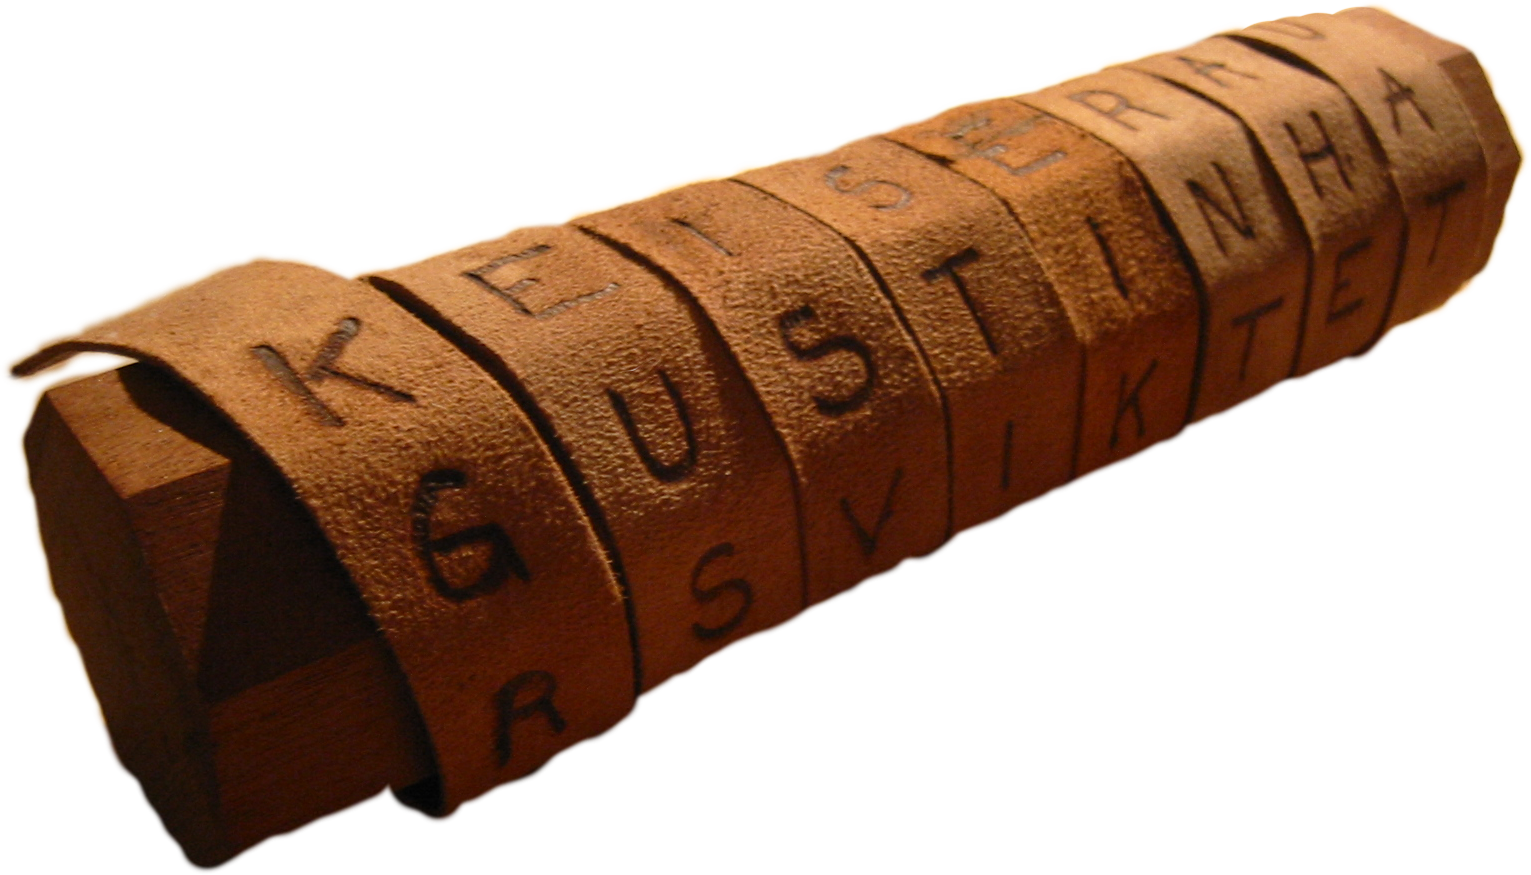
\includegraphics[width=0.60\textwidth]{pic/Skytale}}
	~~
	\subcaptionbox{Аристотель (384 -- 322~гг.~до~н.~э.). Римская копия оригинала Лисиппа}{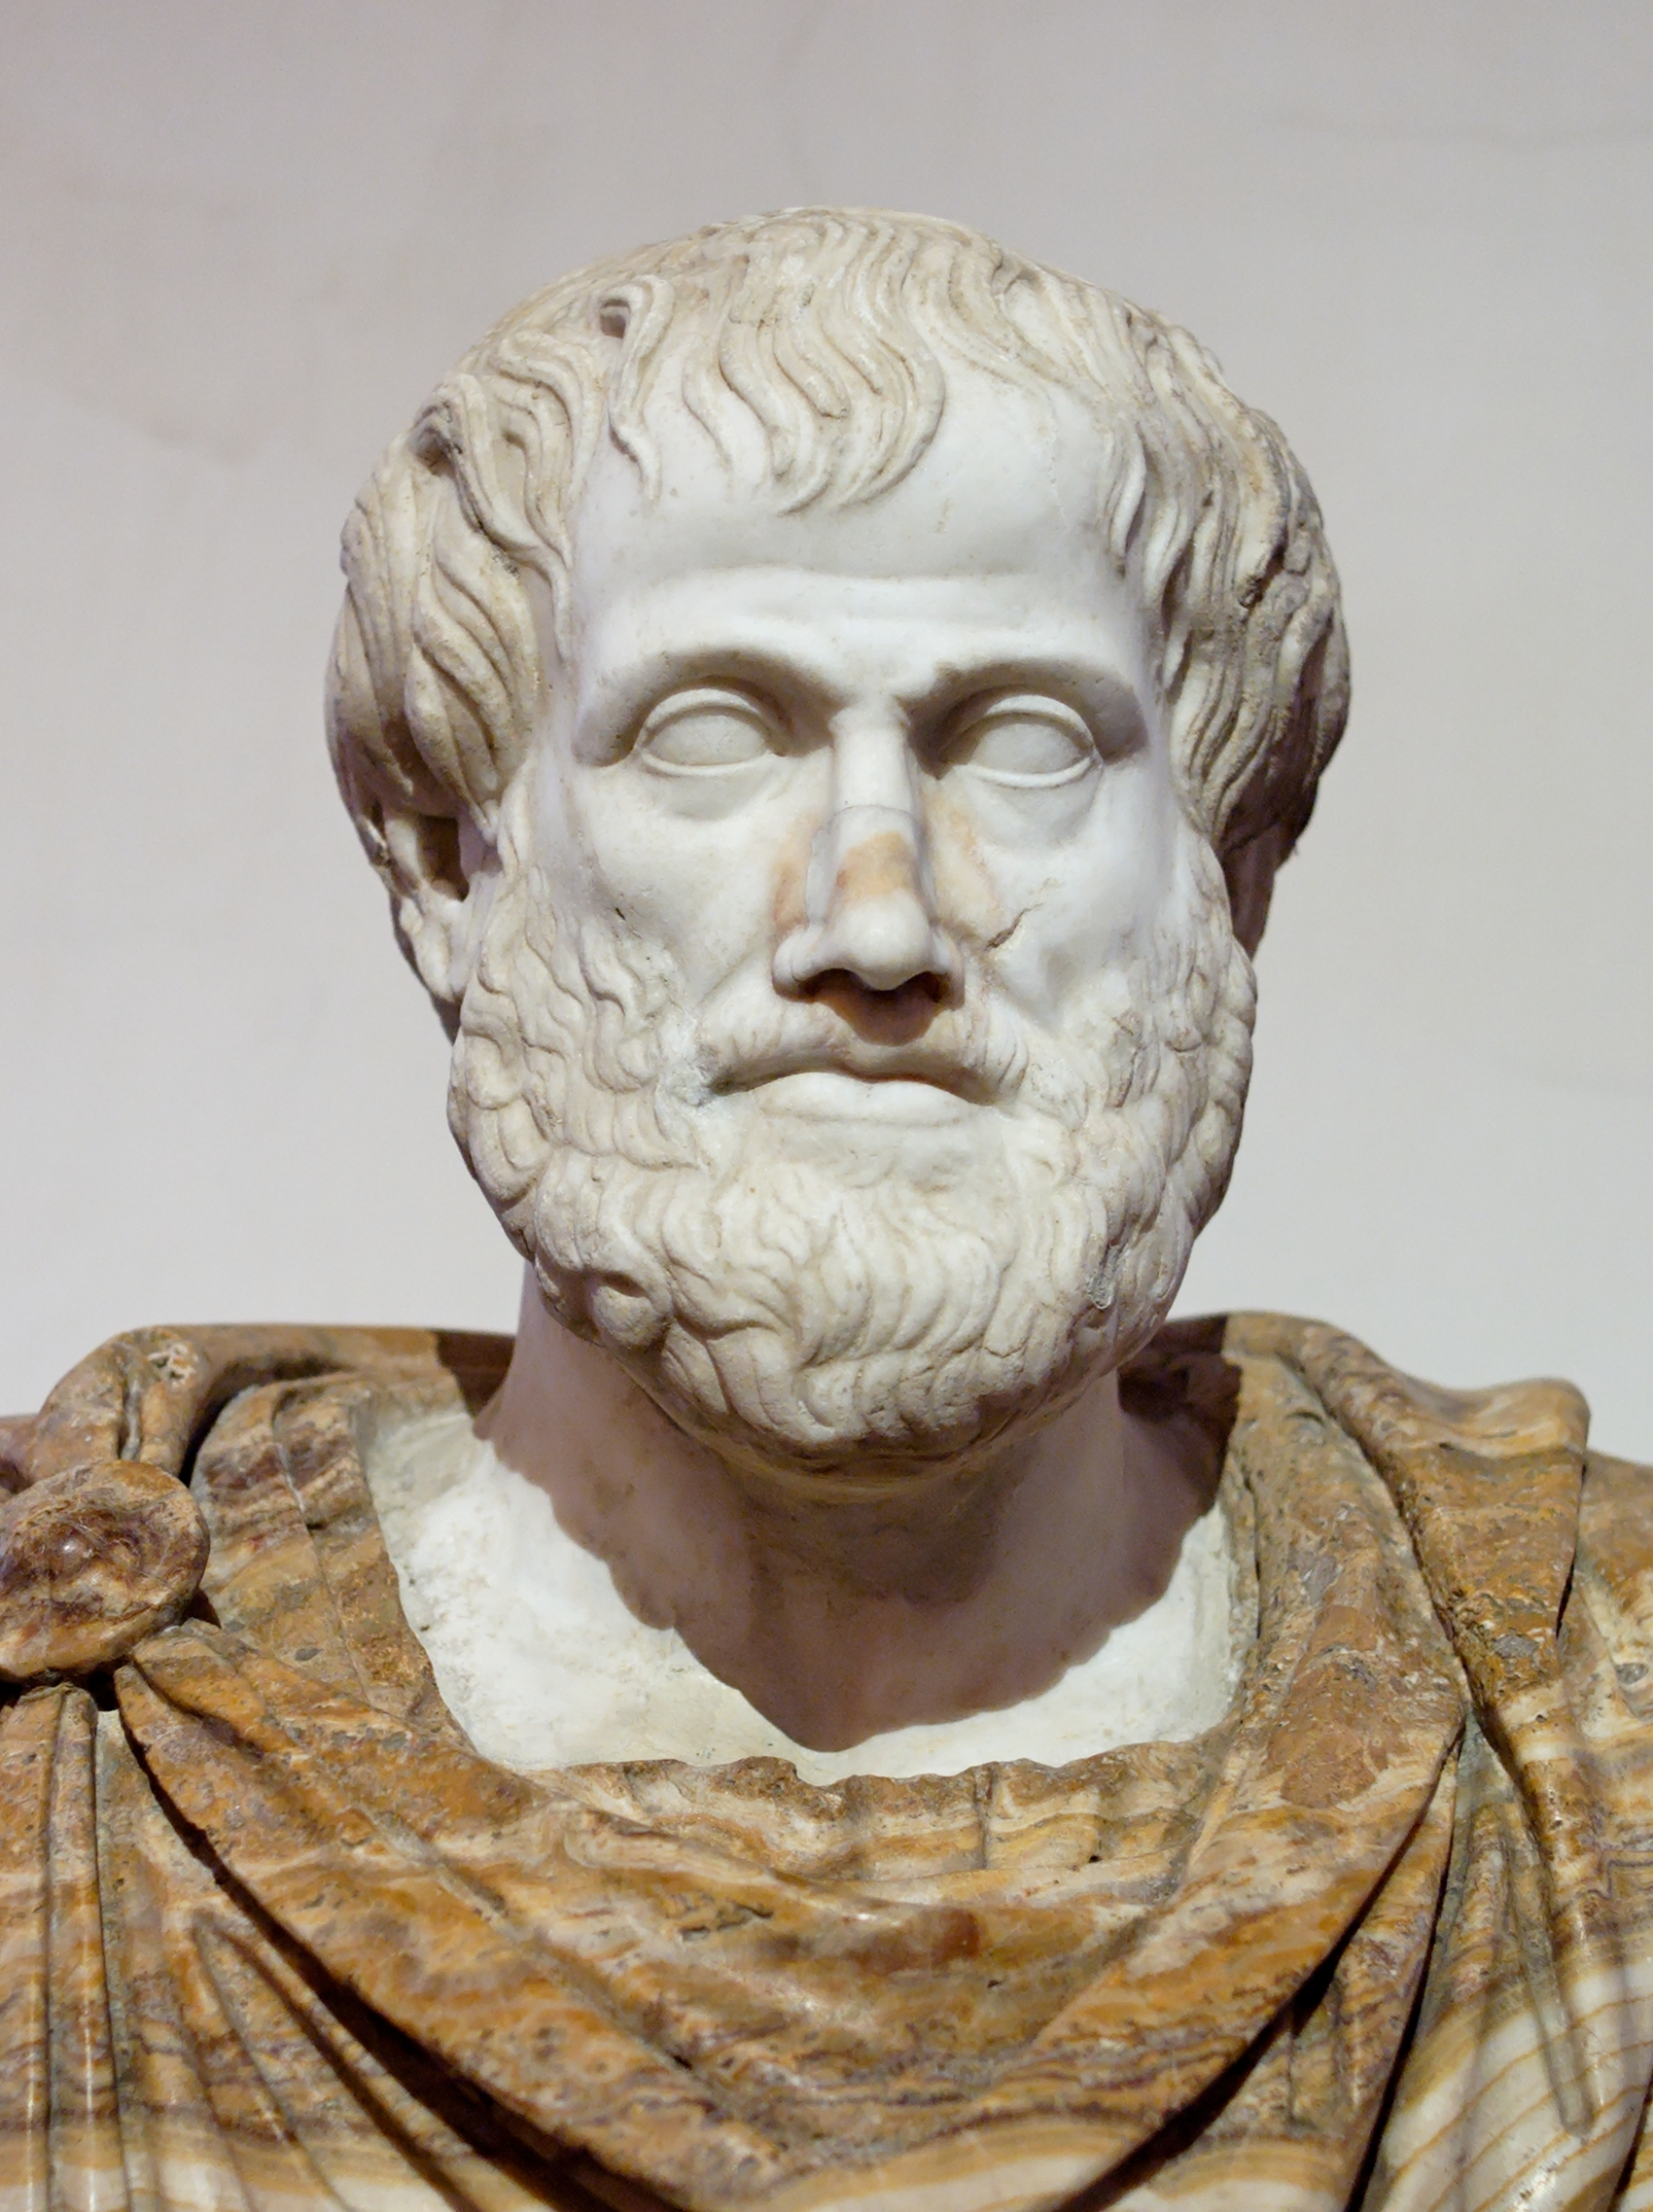
\includegraphics[width=0.35\textwidth]{pic/Aristotle_Altemps_Inv8575}}
	\caption{Скитала\index{скитала}, <<шифр Древней Спарты>>\index{шифр!Древней Спарты}}
\end{figure}

В Ветхом Завете, в том числе в книге пророка Иеремии (VI~век до~н.~э.), использовалась техника скрытия отдельных кусков текста, получившая название <<атбаш>>\index{шифр!атбаш}.

\begin{itemize}
	\item \texttt{Иер. 25:26}: и всех царей севера, близких друг к другу и дальних, и все царства земные, которые на лице земли, а царь Сесаха выпьет после них.
	\item \texttt{Иер. 51:41}: Как взят Сесах, и завоевана слава всей земли! Как сделался Вавилон ужасом между народами!
\end{itemize}

В этих отрывках слово <<Сесах>> относится к государству, неупоминаемому в других источниках, но если в написании слова <<Сесах>> на иврите (\cjRL{/s/sK}) заменить первую букву алфавита на последнюю, вторую на предпоследнюю и так далее, то получится <<Бавель>> (\cjRL{bbl}) -- одно из названий Вавилона. Таким образом, с помощью техники <<атбаш>> авторы манускрипта скрывали отдельные названия, оставляя б\'{о}льшую часть текста без шифрования. Возможно, это делалось в том числе и для того, чтобы не иметь проблем с распространением текстов на территории, подконтрольной Вавилону. Шифр <<атбаш>>\index{шифр!атбаш} можно рассматривать как пример моноалфавитного афинного шифра (см. раздел~\ref{section-affine-cipher}).

Сразу несколько техник защищённой передачи сообщений связывают с именем Энея Тактика, полководца IV~века до~н.~э.
\begin{itemize}
	\item \emph{Диск Энея} представлял собой диск небольшого диаметра с отверстиями, которые соответствовали буквам алфавита. Отправитель протягивал нитку через отверстия, тем самым кодируя сообщение. Диск с ниткой отправлялся получателю. Особенностью диска Энея было то, что, в случае захвата гонца, последний мог быстро выдернуть нитки из диска, фактически уничтожив передаваемое сообщение.
	\item \emph{Линейка Энея} представляла собой линейку с отверстиями, соответствующими буквам греческого алфавита. Нитку также продевали через отверстия, тем самым шифруя сообщение. Однако после продевания на нитке завязывали узлы. После окончания нитку снимали с линейки и отправляли получателю. Чтобы восстановить сообщение, получатель должен был иметь линейку с таким же порядком отверстий, как та, на которой текст шифровался. Подобный метод можно назвать моноалфавитным шифром (см. раздел~\ref{section-substitution-cipher}), исходное сообщение -- открытым текстом, нитку с узлами -- шифртекстом, а саму линейку -- ключом шифрования.
	\item Ещё одна техника, \emph{книжный шифр Энея}, состояла в прокалывании небольших отверстий в книге или манускрипте рядом с буквами, соответствующими буквам исходного сообщения. Этот метод относится уже не к криптографии, а к стеганографии -- науке о скрытии факта передачи сообщения.
\end{itemize}

Ко II~веку до~н.~э. относят изобретение в Древней Греции квадрата Полибия (рис.~\ref{fig:polubios-square}). Метод позволял передавать информацию на большие расстояния с помощью факелов. Каждой букве алфавита ставилось в соответствие два числа от 1 до 5 (номера строки и столбца в квадрате Полибия). Эти числа обозначали количество факелов, которое было необходимо поднять на сигнальной башне. Квадрат Полибия относится к методам кодирования информации: переводу информации из одного представления (греческого алфавита) в другое (число факелов) для удобства хранения, обработки или передачи.

\begin{figure}[t]
	\centering
\begin{tabular}{ || c || c | c | c | c | c ||}
\hline
\hline
  & 1 & 2 & 3 & 4 & 5 \\
\hline
\hline
1 & A & B & $\Gamma$ & $\Delta$ & E \\
\hline
2 & Z & H & $\Theta$ & I & K \\
\hline
3 & $\Lambda$ & M & N & $\Xi$ & O  \\
\hline
4 & $\Pi$ & P & $\Sigma$ & T & $\Upsilon$ \\
\hline
5 & $\Phi$ & X & $\Psi$ & $\Omega$ & \\
\hline
\hline
\end{tabular}
  \caption{Квадрат Полибия для греческого алфавита}
  \label{fig:polubios-square}
\end{figure}

Известен метод шифрования, который использовался Гаем Юлием Цезарем (100--44~гг.~до~н.~э.). Он получил название <<шифр Цезаря>>\index{шифр!Цезаря} и состоял в замене каждой буквы текста на другую букву, следующую в алфавите через две позиции (см. раздел~\ref{section-caesar-cipher}). Данный метод относится к классу моноалфавитных шифров.

В VIII веке~н.~э. была опубликована <<Книга тайного языка>> Аль-Халиля аль-Фарахиди, в которой арабский филолог описал технику криптоанализа, сейчас известную как атака по открытому тексту. Он предположил, что первыми словами письма, которое было отправлено византийскому императору, была фраза <<Во имя Аллаха>>, что оказалось верным и позволило расшифровать оставшуюся часть письма. Абу аль-Кинди (801--873~гг.~н.~э.) в своём <<Трактате о дешифровке криптографических сообщений>> показал, что моноалфавитные шифры, в которых каждому символу кодируемого текста ставится в однозначное соответствие какой-то другой символ алфавита, легко поддаются частотному криптоанализу. В тексте трактата аль-Кинди привёл таблицу частот букв, которую можно использовать для дешифровки шифртекстов на арабском языке, использующих моноалфавитный шифр.

\begin{figure}[t]
	\centering
	\subcaptionbox{Статуя Леона Баттиста Альберти (\langit{Leone Battista Alberti}, 1404--1472) во дворе Уффици. Фото участника it.wiki Frieda, доступно по \href{https://creativecommons.org/licenses/by-sa/3.0/deed.ru}{лицензии CC-BY-SA 3.0}}{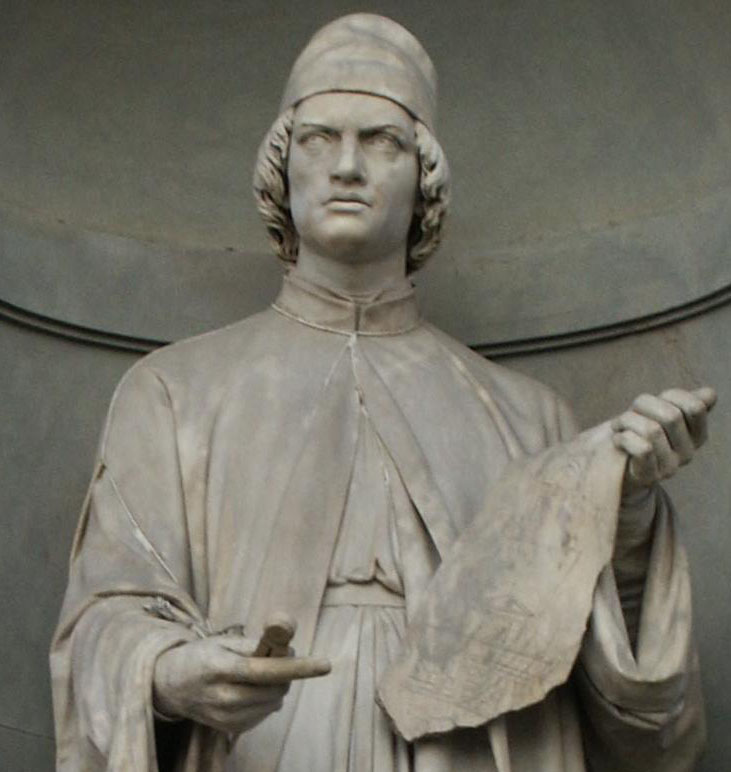
\includegraphics[width=0.50\textwidth]{pic/Leon_Battista_Alberti_1}}
	~
	\subcaptionbox{Фрагмент оформления гробницы Иоганна Тритемия (\langlat{Iohannes Trithemius}, 1462--1516)}{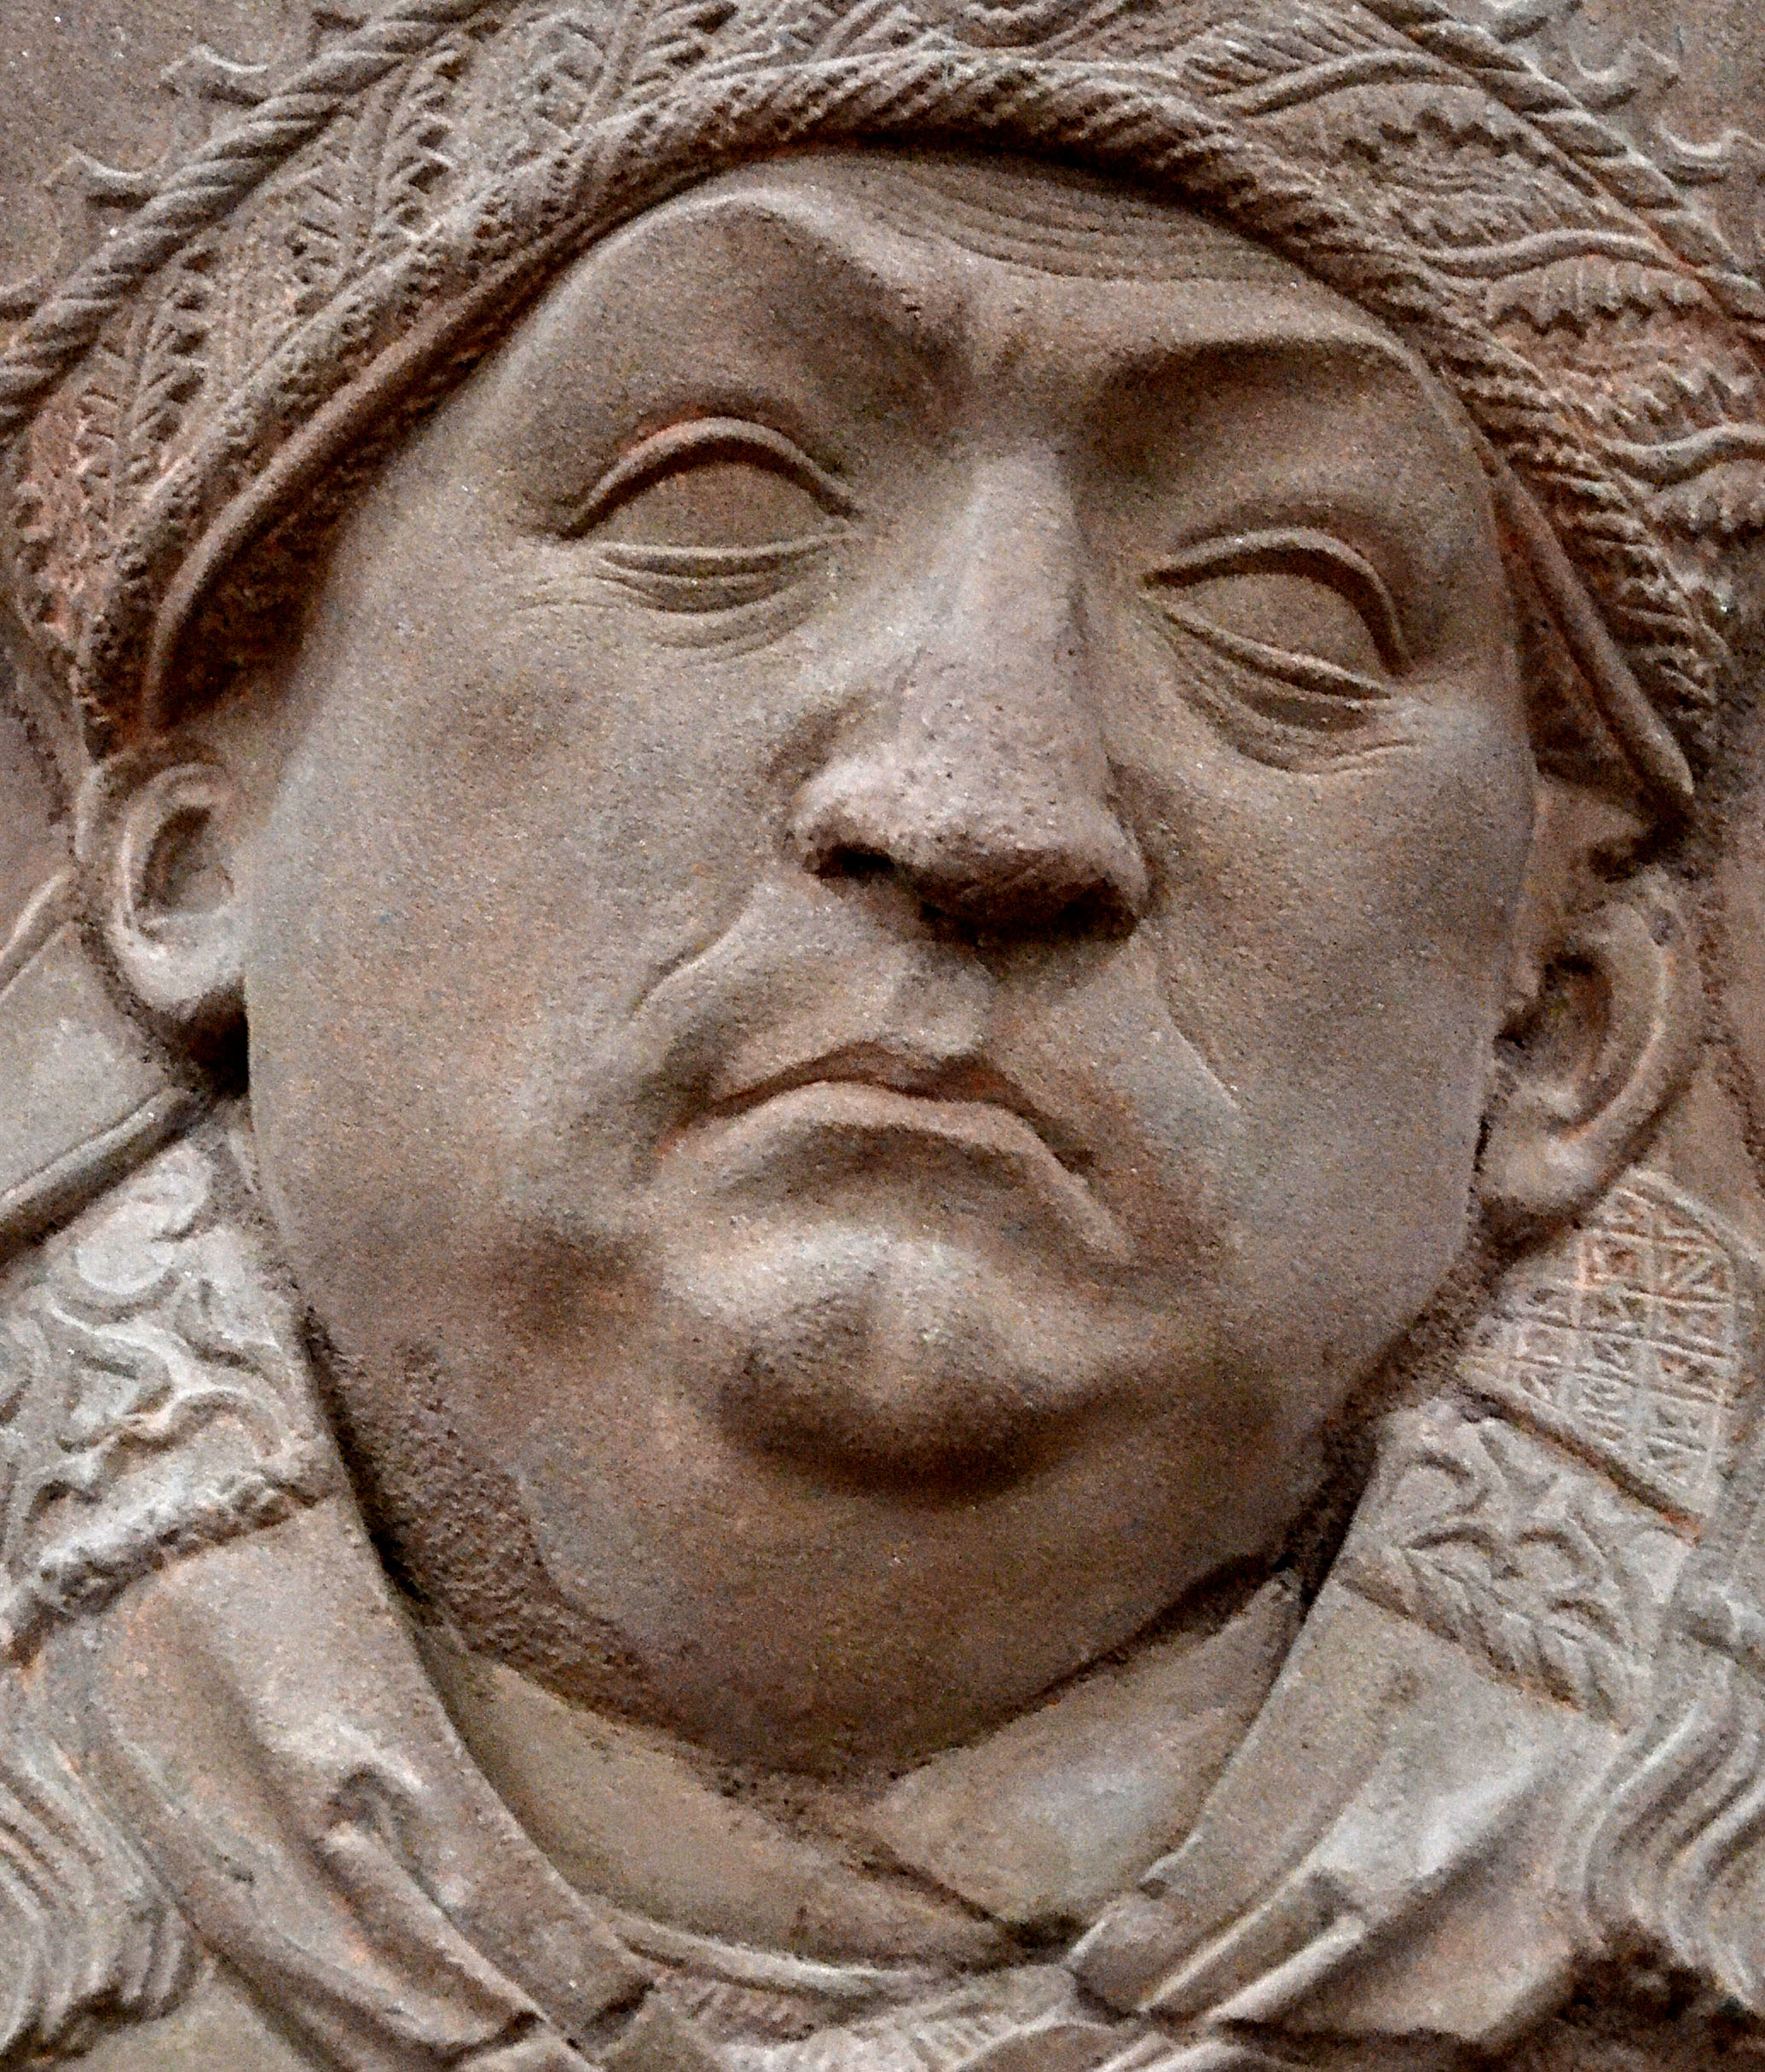
\includegraphics[width=0.45\textwidth]{pic/Trithemiusmoredetail}}
	\caption{Отцы западной криптографии}
\end{figure}

Итальянский архитектор Леон Баттиста Альберти, проанализировав использовавшиеся в Европе шифры, предложил для каждого текста использовать не один, а несколько моноалфавитных шифров. Однако Альберти не смог предложить законченной идеи полиалфавитного шифра, хотя его и называют отцом западной криптографии. В истории развития полиалфавитных шифров до XX века также наиболее известны немецкий аббат XVI века Иоганн Тритемий и английский учёный XIX века Чарльз Уитстон (\langen{Charles Wheatstone}, 1802--1875). Уитстон изобрёл простой и стойкий способ полиалфавитной замены, называемый шифром Плейфера\index{шифр!Плейфера} в честь лорда Плейфера, способствовавшего внедрению шифра. Шифр Плейфера использовался вплоть до Первой мировой войны.

\begin{figure}[t]
	\centering
	\subcaptionbox{<<Энигма>>\label{fig:enigma}}{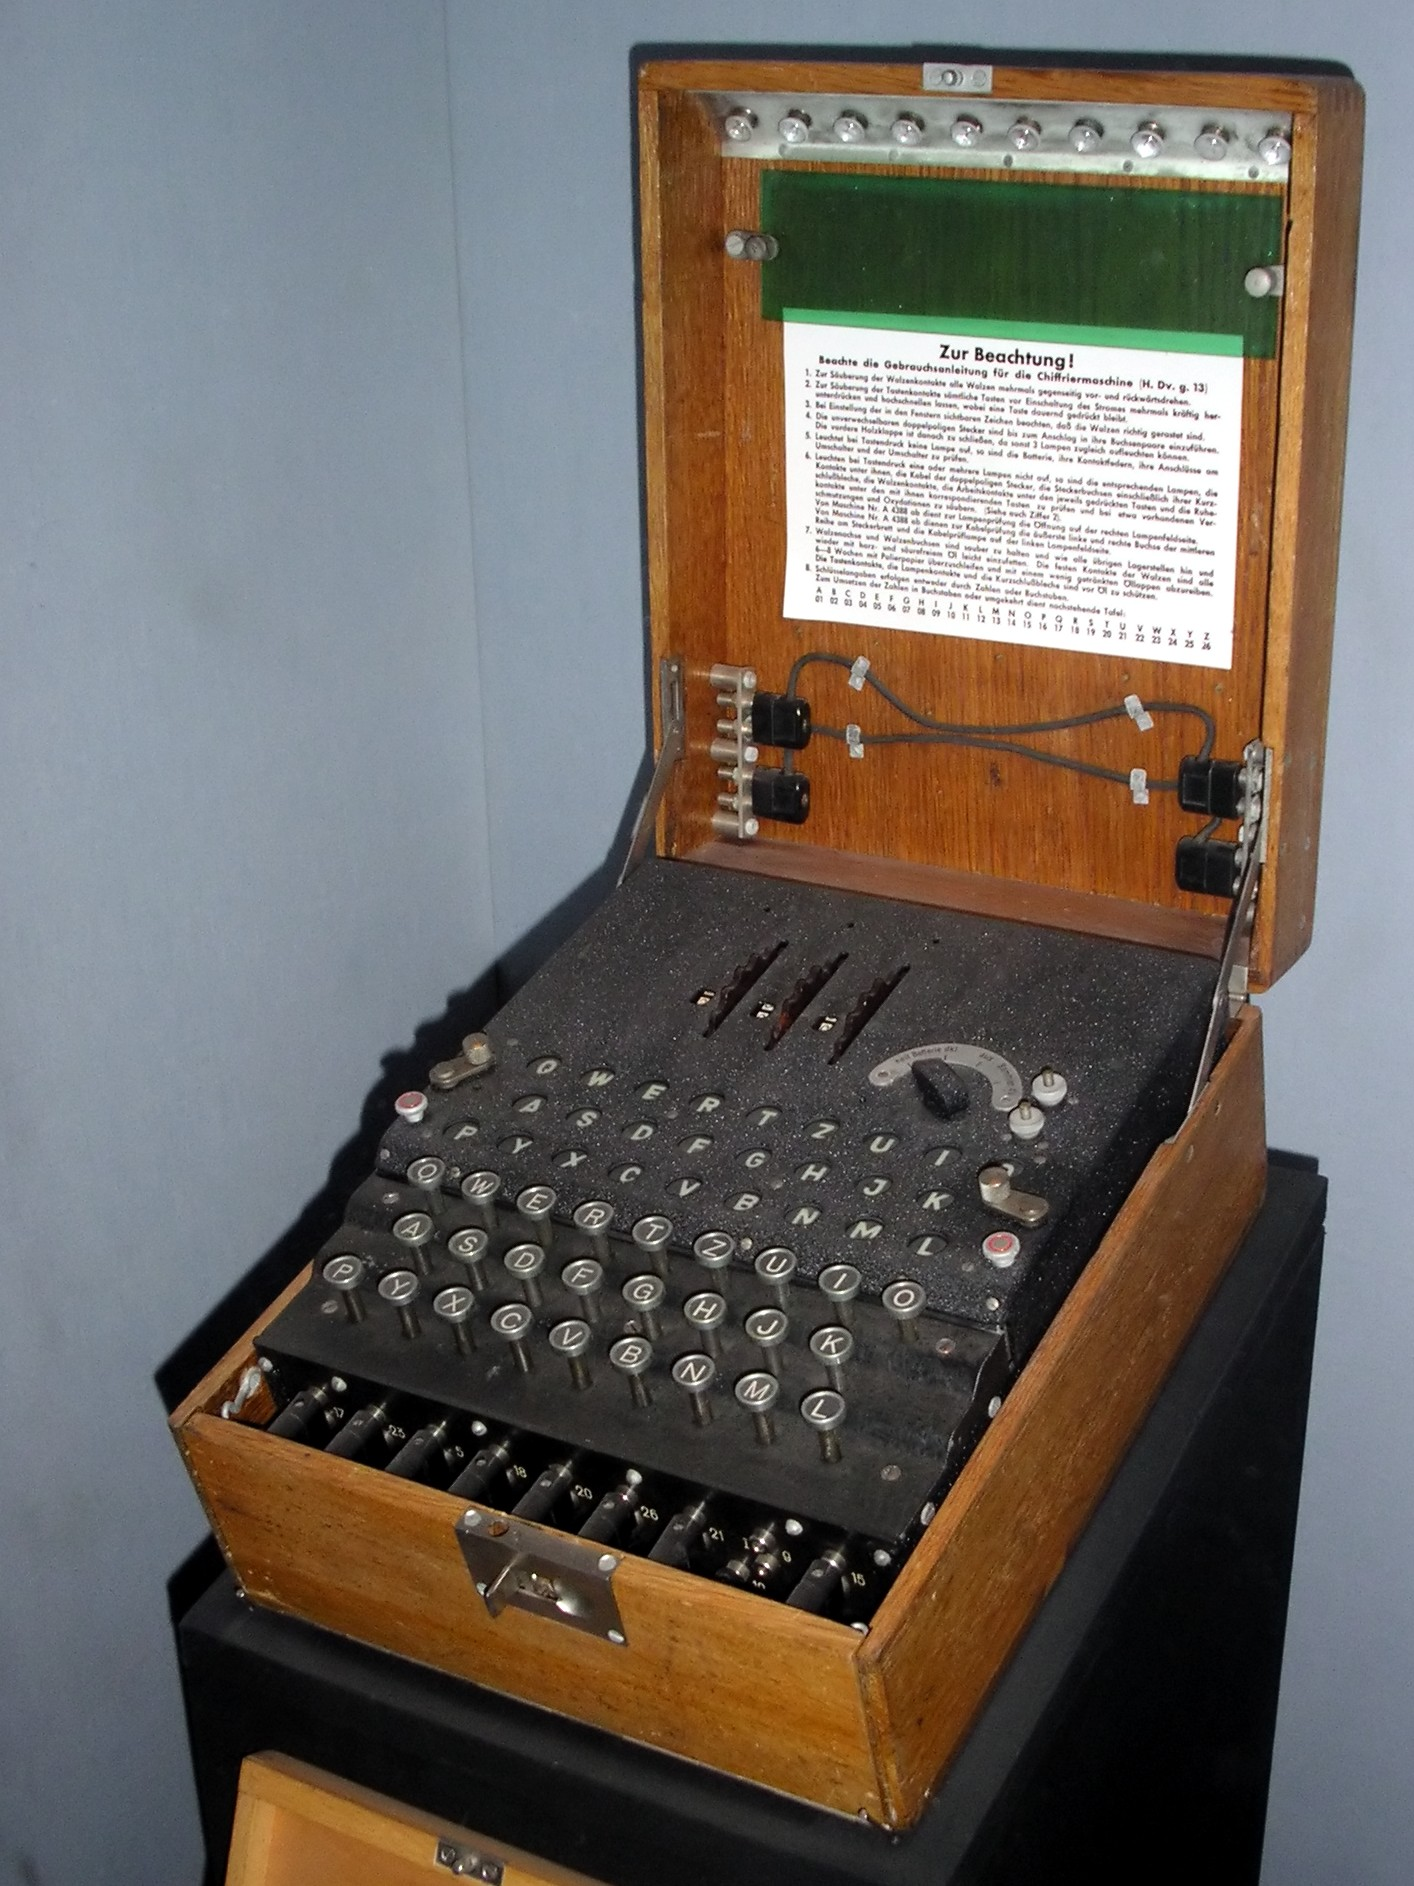
\includegraphics[width=0.35\textwidth]{pic/EnigmaMachine}}
	~~
	\subcaptionbox{<<Лоренц>> (без кожуха)\label{fig:lorenz}}{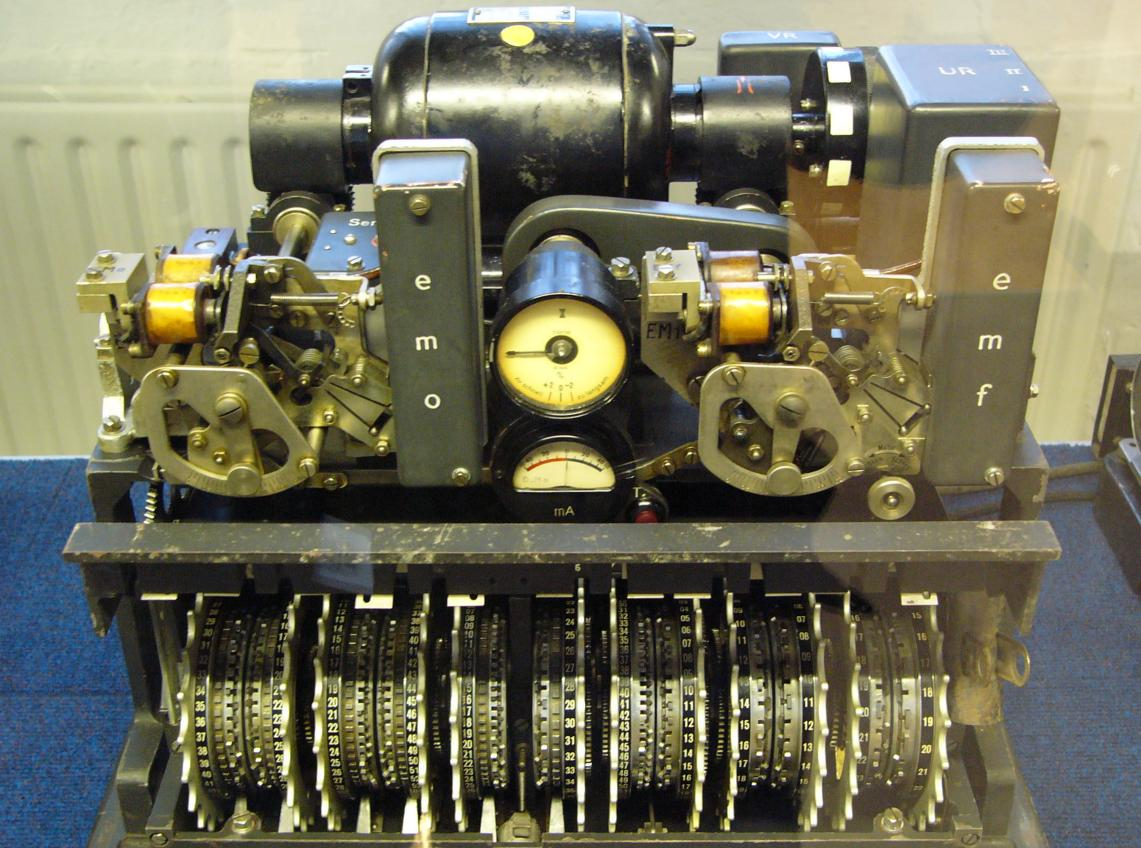
\includegraphics[width=0.60\textwidth]{pic/Lorenz-SZ42-2}}
	\caption{Криптографические машины Второй мировой войны}
\end{figure}

Роторные машины XX века позволяли создавать и реализовывать устойчивые к <<наивному>> взлому полиалфавитные шифры. Примером такой машины является немецкая <<Энигма>>\index{Энигма}, разработанная в конце Первой мировой войны (рис.~\ref{fig:enigma}). Период активного применения <<Энигмы>> пришёлся на Вторую мировую войну. Хотя роторные машины использовались в промышленных масштабах, криптография, на которой они были основаны, представляла собой всё ещё искусство, а не науку. Отсутствовал научный базис надёжности криптографических инструментов. Возможно, это было одной из причин успеха криптоанализа <<Энигмы>>, который сначала был достигнут в Польше в <<Бюро шифров>>, а потом и в <<Блетчли-парке>> в Великобритании. Польша впервые организовала курсы криптографии не для филологов и специалистов по немецкому языку, а для математиков, хотя и знающих язык весьма вероятного противника. Трое из выпускников курса -- Мариан Реевский, Генрих Зыгальский и Ежи Рожицкий -- поступили на службу в «Бюро шифров» и получили первые результаты успешного криптоанализа. Используя математику, электромеханические приспособления и данные французского агента Asche (Ганс-Тило Шмидт), они могли дешифровывать значительную часть сообщений вплоть до лета 1939 года, когда вторжение Германии в Польшу стало очевидным. Дальнейшая работа по криптоанализу <<Энигмы>> в центре британской разведки <<Station~X>>\index{Station X} (<<Блетчли-парк>>\index{Блетчли-парк}) связана с именами таких известных математиков, как Гордон Уэлчман и Алан Тьюринг. Кроме <<Энигмы>> в центре проводили работу над дешифровкой и других шифров, в том числе немецкой шифровальной машины <<Лоренц>> (рис.~\ref{fig:lorenz}). Для целей её криптоанализа был создан компьютер Colossus, имевший 1500 электронных ламп, а его вторая модификация -- Colossus Mark II -- считается первым в мире программируемым компьютером в истории ЭВМ.

Середина XX века считается основной вехой в истории науки о защищённой передаче информации и криптографии. Эта веха связана с публикацией двух статей Клода Шеннона: <<Математическая теория связи>> (\langen{"A Mathematical Theory of Communication"}, 1948, \cite{Shannon:1948:MTCa, Shannon:1948:MTCb}) и <<Теория связи в секретных системах>> (\langen{"Communication Theory of Secrecy Systems"}, 1949, \cite{Shannon:1949:CTS}). В данных работах Шеннон впервые определил фундаментальные понятия в теории информации, а также показал возможность применения этих понятий для защиты информации, тем самым заложив математическую основу современной криптографии.

Кроме того, появление электронно-вычислительных машин кардинально изменило ситуацию в криптографии. С одной стороны, вычислительные способности ЭВМ открыли совершенно новые возможности реализации шифров, недоступных ранее из-за их высокой сложности. С другой стороны, аналогичные возможности стали доступны и криптоаналитикам. Появилась необходимость не только в создании шифров, но и в обосновании того, что новые вычислительные возможности не смогут быть использованы для взлома новых шифров.

В 1976 году появился шифр DES (\langen{Data Encryption Standard})\index{шифр!DES}, который был принят как стандарт США. DES широко использовался для шифрования пакетов данных при передаче в компьютерных сетях и системах хранения данных. С 90-х годов параллельно с традиционными шифрами, основой которых была булева алгебра, активно развиваются шифры, основанные на операциях в конечном поле. Широкое распространение персональных компьютеров и быстрый рост производительности ЭВМ и объёма передаваемых данных в компьютерных сетях привели к замене в 2002 году стандарта DES на более стойкий и быстрый в программной реализации стандарт -- шифр AES (\langen{Advanced Encryption Standard})\index{шифр!AES}. Окончательно DES был выведен из эксплуатации как стандарт в 2005 году.

В беспроводных голосовых сетях передачи данных используются шифры с малой задержкой шифрования и расшифрования на основе посимвольных преобразований -- так называемые \emph{потоковые шифры}\index{шифр!потоковый}.

Параллельно с разработкой быстрых шифров в 1976~г. появился новый класс криптосистем, так называемые \emph{криптосистемы с открытым ключом}\index{криптосистема!с открытым ключом}. Хотя эти новые криптосистемы намного медленнее и технически сложнее симметричных, они открыли принципиально новые возможности: создание общего ключа с использованием открытого канала и \emph{электронной подписи}, которые составили основу современной защищённой связи в Интернете.



\section{Основные понятия}
\selectlanguage{russian}
Для успешного выполнения любых целей по защите информации необходимо участие в процессе защиты нескольких субъектов, которые по определённым правилам будут выполнять технические или организационные действия, криптографические операции, взаимодействовать друг с другом, например, передавая сообщения или проверяя личности друг друга.

Формализация подобных действий делается через описание протокола. \emph{Протокол} -- описание распределённого алгоритма, в процессе выполнения которого два или более участников последовательно выполняют определённые действия и обмениваются сообщениями\footnote{Здесь и далее в этом разделе определения даны на основе~\cite{Cheremushkin:2009}.}.

Под участником\index{участник!протокола} (субъектом\index{субъект!протокола}, стороной\index{сторона!протокола}) протокола понимают не только людей, но и приложения, группы людей или целые организации. Формально участниками считают только тех, кто выполняет активную роль в рамках протокола. Хотя при создании и описании протоколов забывать про пассивные стороны тоже не стоит. Например, пассивный криптоаналитик\index{криптоаналитик!пассивный} формально не является участником протоколов, но многие протоколы разрабатываются с учётом защиты от таких <<неучастников>>.

Протокол состоит из \emph{циклов}\index{цикл!протокола} (\langen{round}) или \emph{проходов}\index{проход!протокола} (\langen{pass}). Цикл -- временной интервал активности только одного участника. За исключением самого первого цикла протокола, обычно начинается приёмом сообщения, а заканчивается -- отправкой.

Цикл (или проход) состоит из \emph{шагов} (действий, \langen{step, action}) -- конкретных законченных действий, выполняемых участником протокола. Например:
\begin{itemize}
	\item генерация нового (случайного) значения;
	\item вычисление значений функции;
	\item проверка сертификатов, ключей, подписей, и др.;
	\item приём и отправка сообщений.
\end{itemize}

Прошедшая в прошлом или даже просто теоретически описанная реализация протокола для конкретных участников называется \emph{сеансом}\index{сеанс!протокола}. Каждый участник в рамках сеанса выполняет одну или несколько \emph{ролей}. В другом сеансе протокола участники могут поменяться ролями и выполнять уже совсем другие функции.

Можно сказать, что протокол прескрептивно описывает правила поведения каждой роли в протоколе. А сеанс это дескриптивное описание (возможно теоретически) состоявшейся в прошлом реализации протокола.

Пример описания протокола.
\begin{enumerate}
	\item Участник с ролью <<Отправитель>> должен отправить участнику с ролью <<Получатель>> сообщение.
	\item Участник с ролью <<Получатель>> должен принять от участника с ролью <<Отправитель>> сообщение.
\end{enumerate}

Пример описания сеанса протокола.
\begin{enumerate}
	\item 1-го апреля в 13:00 Алиса отправила Бобу сообщение.
	\item 1-го апреля в 13:05 Боб принял от Алисы сообщение.
\end{enumerate}

\emph{Защищённым протоколом}\index{протокол!защищённый} или \emph{протоколом обеспечения безопасности}\index{протокол!обеспечения безопасности} будет называть протокол, обеспечивающий выполнение хотя бы одной защитной функции~\cite{ISO:7498-2:1989}:
\begin{itemize}
	\item аутентификация сторон и источника данных,
	\item разграничение доступа,
	\item конфиденциальность,
	\item целостность,
	\item невозможность отказа от факта отправки или получения.
\end{itemize}

Если защищённый протокол предназначен для выполнения функций безопасности криптографической системы, или если в процессе его исполнения используются криптографические алгоритмы, то такой протокол будем называть \emph{криптографическим}\index{протокол!криптографический}.


\chapter{Классические шифры}

В главе приведены наиболее известные \emph{классические} шифры, которыми можно было пользоваться до появления роторных машин. К ним относятся такие шифры, как шифр Цезаря\index{шифр!Цезаря}, шифр Плейфера\index{шифр!Плейфера}, шифр Хилла\index{шифр!Хилла} и шифр Виженера\index{шифр!Виженера}. Они наглядно демонстрируют различные классы шифров.

\input{monoalphabetic_ciphers}

\section{Биграммные шифры замены}\index{шифр!биграммный}
\selectlanguage{russian}

Если при шифровании преобразуется по две буквы открытого текста, то такой шифр называется \emph{биграммным}\index{шифр!биграммный} шифром замены. Первый биграммный шифр был изобретён аббатом Иоганном Тритемием и опубликован в 1508-м году. Другой биграммный шифр изобретён в 1854 году Чарльзом Витстоном. Лорд Лайон Плейфер (\langen{Lyon Playfair}) внедрил этот шифр в государственных службах Великобритании, и шифр был назван шифром Плейфера\index{шифр!Плейфера}.

Опишем шифр Плейфера\index{шифр!Плейфера}. Составляется таблица для английского алфавита (буквы \texttt{I}, \texttt{J} отождествляются), в которую заносятся буквы перемешанного алфавита, например, в виде таблицы, представленной ниже. Часто перемешивание алфавита реализуется с помощью начального слова, в котором отбрасываются повторяющиеся символы. В нашем примере начальное слово \texttt{playfair}. Таблица имеет вид:

\begin{center}
    \begin{tabular}{ccccc}
        p & l & a & y & f  \\
        i & r & b & c & d  \\
        e & g & h & k & m  \\
        n & o & q & s & t  \\
        u & v & w & x & z  \\
    \end{tabular}
\end{center}

Буквы открытого текста разбиваются на пары. Правила шифрования каждой пары состоят в следующем.

\begin{itemize}
    \item Если буквы пары не лежат в одной строке или в одном столбце таблицы, то они заменяются буквами, образующими с исходными буквами вершины прямоугольника. Первой букве пары соответствует буква таблицы, находящаяся в том же столбце. Пара букв открытого текста \texttt{we} заменяется двумя буквами таблицы \texttt{hu}. Пара букв открытого текста \texttt{ew} заменяется двумя буквами таблицы \texttt{uh}.
    \item Если буквы пары открытого текста расположены в одной строке таблицы, то каждая буква заменяется соседней справа буквой таблицы. Например, пара \texttt{gk} заменяется двумя буквами \texttt{hm}. Если одна из этих букв -- крайняя правая в таблице, то её <<правым соседом>> считается крайняя левая в этой строке. Так, пара \texttt{to} заменяется буквами \texttt{nq}.
    \item Если буквы пары лежат в одном столбце, то каждая буква заменяется соседней буквой снизу. Например, пара \texttt{lo} заменяется парой \texttt{rv}. Если одна из этих букв крайняя нижняя, то её <<нижним соседом>> считается крайняя верхняя буква в этом столбце таблицы. Например, пара \texttt{kx} заменяется буквами \texttt{sy}.
    \item Если буквы в паре одинаковые, то между ними вставляется определённая буква, называемая <<буквой-пустышкой>>. После этого разбиение на пары производится заново.
\end{itemize}

\example
Используем шифр Плейфера\index{шифр!Плейфера} и зашифруем сообщение "\texttt{Wheatstone was the inventor}". Исходное сообщение, разбитое на биграммы, показано в первой строке таблицы. Результат шифрования, также разбитый на биграммы, приведён во второй строке.
\begin{center} \begin{tabular}{|*{12}c|}
    \hline
    wh & ea & ts & to & ne & wa & st & he & in & ve & nt & or \\
    \hline
    aq & ph & nt & nq & un & ab & tn & kg & eu & gu & on & vg \\
    \hline
\end{tabular} \end{center}
\exampleend

Шифр Плейфера\index{шифр!Плейфера} не является криптографически стойким. Несложно найти ключ, если известны пара открытого текста и соответствующего ему шифртекста. Если известен только шифртекст, криптоаналитик может проанализировать соответствие между частотой появления биграмм в шифртексте и известной частотой появления биграмм в языке, на котором написано сообщение. Такой частотный анализ помогает дешифрованию.


\input{hills_cipher}

% \subsection{Омофонные замены}
%
% Омофонными заменами называют криптопримитивы, в основе которых лежит замена групп символов открытого текста $M$ на группу символов $C$ с использованием ключа $K$. Такой метод шифрования вносит неоднозначность между $M$ и $C$, это позволяет защититься от методов частотного криптоанализа.
%  \subsection{шифрокоды}
%  Шифрокоды -- это класс шифров сочетающих в себе свойства кодов и помехозащищённости со свойствами шифра и обеспечения конфиденциальности.

\input{vigeneres_cipher}

\input{polyalphabetic_cipher_cryptanalysis}

\input{perfect_secure_systems}

\chapter{Блочные шифры}\label{chapter-block-ciphers}\index{шифр!блочный|(}

\section{Введение и классификация}\label{section-block-ciphers-intro}
\selectlanguage{russian}

Блочные шифры являются основой современной криптографии. Многие криптографические примитивы -- криптографически стойкие генераторы псевдослучайной последовательности (см. главу~\ref{section-crypto-random}), криптографические функции хэширования (см. главу~\ref{chapter-hash-functions}) -- так или иначе основаны на блочных шифрах. А использование медленной криптографии с открытым ключом было бы невозможно по практическим соображениям без быстрых блочных шифров.

Блочные шифры можно рассматривать как функцию преобразования строки фиксированной длины в строку аналогичной длины\footnote{В случае использования недетерминированных алгоритмов, дающих новый результат при каждом шифровании, длина выхода будет больше. Меньше длина выхода быть не может, так как будет невозможно однозначно восстановить произвольное сообщение.} с использованием некоторого ключа, а также соответствующую ей функцию расшифрования:
\[\begin{array}{l}
	C = E_K\left( M \right), \\
	M'= D_K\left( C \right).
\end{array}\]

Данные функции необходимо дополнить требованиями корректности, производительности и надёжности. Во-первых, функция расшифрования должна однозначно восстанавливать произвольное исходное сообщение:
\[ \forall k \in \group{K}, m \in \group{M} \hookrightarrow D_k \left( E_k\left( m \right) \right) = m. \]

Во-вторых, функции шифрования и расшифрования должны быть вычислительно простыми для легальных пользователей (знающих ключ). В-третьих, должно быть невозможно найти открытый текст сообщения по шифртексту без знания ключа, кроме как полным перебором всех возможных ключей расшифрования. Также, что менее очевидно, надёжная функция блочного шифра не должна давать возможность найти ключ шифрования (расшифрования), даже если злоумышленнику известны пары открытого текста и шифртекста. Последнее свойство защищает от атак на основе известного открытого текста\index{атака!с известным открытым текстом} и на основе известного шифртекста\index{атака!с известным шифртекстом}, а также активно используется при построении криптографических функций хэширования в конструкции Миагучи~---~Пренеля\index{конструкция!Миагучи~---~Пренеля}. То есть:
\begin{itemize}
	\item $C = f \left( M, K \right)$ и $M = f \left( C, K \right)$ должны вычисляться быстро (легальные операции);
	\item $M = f \left( C \right)$ и $C = f \left( M \right)$ должны вычисляться не быстрее, чем $\left| \group{K} \right|$ операций расшифрования (шифрования) при условии, что злоумышленник может отличить корректное сообщение (см. выводы к разделу~\ref{section_unicity_distance});
	\item $K = f \left( M, C \right)$ должно вычисляться не быстрее, чем $\left| \group{K} \right|$ операций шифрования.
\end{itemize}

Если размер ключа достаточно большой (от 128 бит и выше), то функцию блочного шифрования, удовлетворяющую указанным выше условиям, можно называть надёжной.

Блочные шифры делят на два больших класса по методу построения.
\begin{itemize}
	\item Шифры, построенные на SP-сетях (сети замены-пере\-становки). Такие шифры основаны на \emph{обратимых} преобразованиях с открытым текстом. При их разработке криптограф должен следить за тем, чтобы каждая из производимых операций была и криптографически надёжна, и обратима при знании ключа.
	\item Шифры, в той или иной степени построенные на ячейке Фейстеля\index{ячейка Фейстеля}. В данных шифрах используется конструкция под названием <<ячейка Фейстеля>>, которая по методу построения уже обеспечивает обратимость операции шифрования легальным пользователем при знании ключа. Криптографу при разработке функции шифрования остаётся сосредоточиться на надёжности конструкции.
\end{itemize}

Все современные блочные шифры являются \emph{раундовыми} (см. рис.~\ref{fig:block-cipher}). То есть блок текста проходит через несколько одинаковых (или похожих) преобразований, называемых \emph{раундами шифрования}. У~функции шифрования также могут существовать начальный и завершающий раунды, отличающиеся от остальных (обычно -- отсутствием некоторых преобразований, которые не имеют смысла для <<крайних>> раундов).

\begin{figure}[!t]
	\centering
	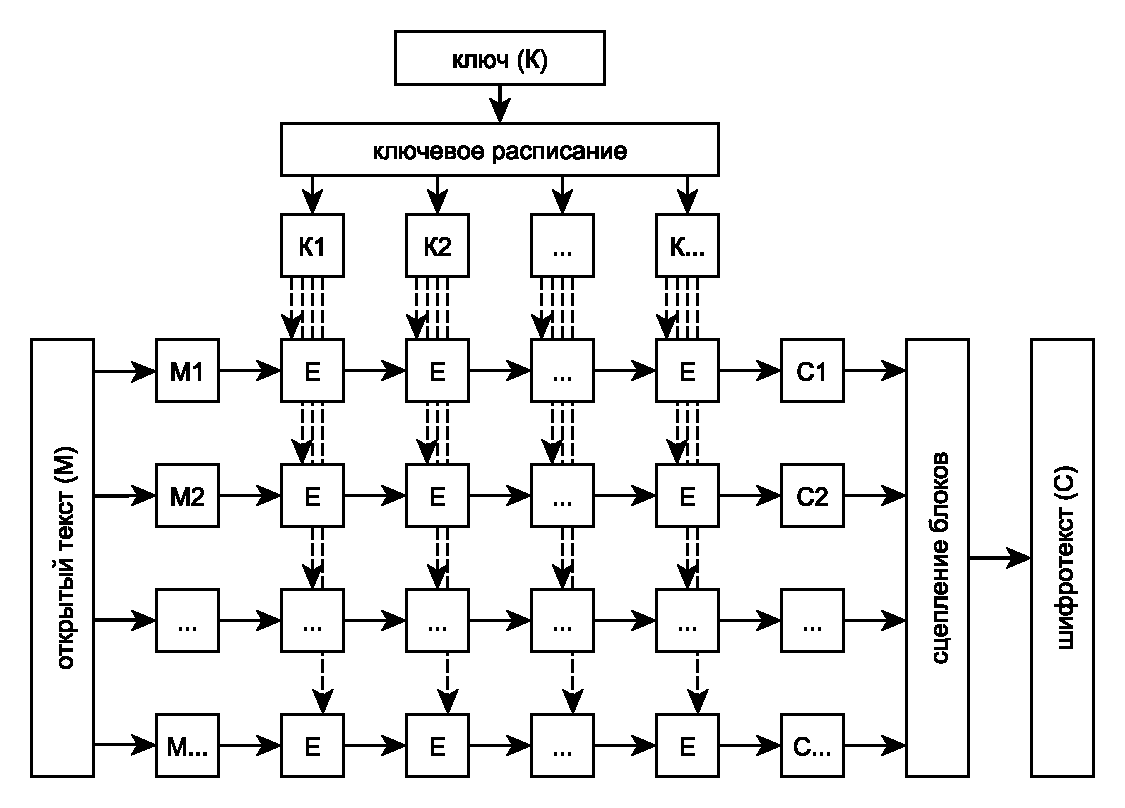
\includegraphics[width=1\textwidth]{pic/block-cipher}
  \caption{Общая структура раундового блочного шифра. С помощью функции ключевого расписания из ключа $K$ получается набор раундовых ключей $K1, K2, \dots$. Открытый текст $M$ разбивается на блоки $M1, M2, \dots$, каждый из которых проходит несколько раундов шифрования, используя соответствующие раундовые ключи. Результаты последних раундов шифрования каждого из блоков объединяются в шифртекст $C$ с помощью одного из режимов сцепления блоков}
  \label{fig:block-cipher}
\end{figure}

Аргументами каждого раунда являются результаты предыдущего раунда (для первого -- часть открытого текста) и \emph{раундовый ключ}\index{ключ!раундовый}. Раундовые ключи получаются из оригинального ключа шифрования с помощью процедуры, получившей название алгоритма \emph{ключевого расписания}\index{ключевое расписание} (также встречаются названия <<расписание ключей>>, <<процедура расширения ключа>> и~др.; \langen{key schedule}). Функция ключевого расписания является важной частью блочного шифра. На потенциальной слабости этой функции основаны такие криптографические атаки, как атака на основе связанных ключей\index{атака!на связанных ключах} и атака скольжения\index{атака!скольжения}.

После прохождения всех раундов шифрования блоки $C1$, $C2$,~$\dots$ объединяются в шифртекст $C$ с помощью одного из режимов сцепления блоков (см. раздел~\ref{section-block-chaining}). Простейшим примером режима сцепления блоков является режим электронной кодовой книги\index{режим!электронной кодовой книги}, когда блоки $C1$, $C2$,~$\dots$ просто конкатенируются в шифртекст $C$ без дополнительной обработки.

К числовым характеристикам блочного шифра относят:
\begin{itemize}
	\item размер входного и выходного блоков,
	\item размер ключа шифрования,
	\item количество раундов.
\end{itemize}

Также надёжные блочные шифры обладают \emph{лавинным эффектом}\index{лавинный эффект} (\langen{avalanche effect}): изменение одного бита в блоке открытого текста или ключа приводит к полному изменению соответствующего блока шифртекста.


\section{SP-сети. Проект «Люцифер»}\label{section-project-lucifer}\index{шифр!Люцифер|(}
\selectlanguage{russian}

В 1973 году в журнале \foreignlanguage{english}{``Scientific American''} появилась статья сотрудника IBM (а ранее -- ВМС США) Хорста Фейстеля (\langen{Horst Feistel}) <<Cryptography and Computer Privacy>>~\cite{Feistel:1973}, описывающая проект функции шифрования <<Люцифер>>, который можно считать прообразом современных блочных шифров. Развитием данной системы стал государственный стандарт США <<Digital Encryption Standard>> с 1979 по 2001 годы.

\begin{figure}[!t]
    \centering
    \subcaptionbox{S-блок. На вход поступают 3 бита информации, которые трактуются как двоичное представление номера одной из $2^3$ линий внутреннего p-блока. На выходе номер активной сигнальной дорожки обратно преобразуется в 3-битовое представление\label{fig:s-box-inside}}{ 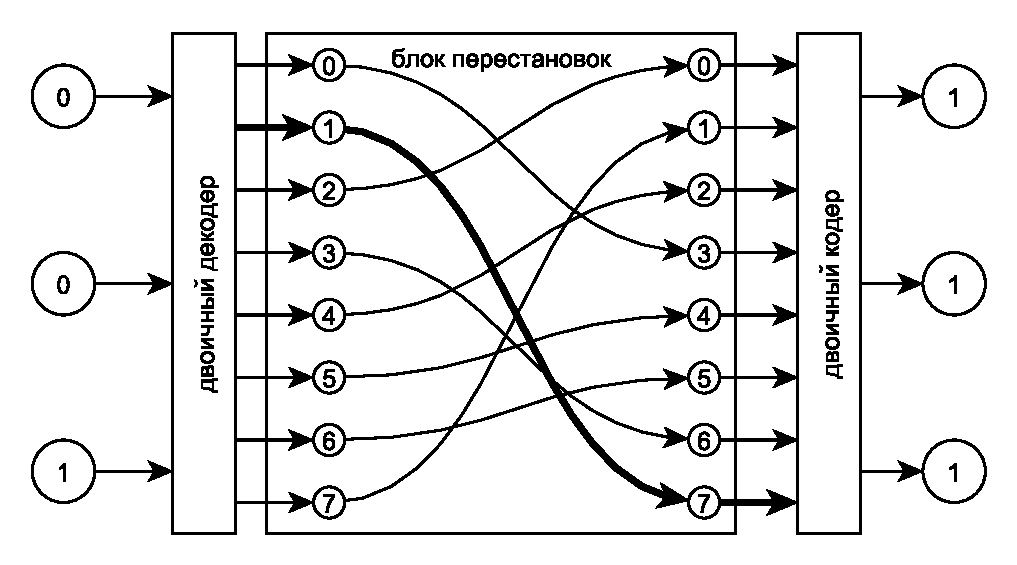
\includegraphics[width=0.66\textwidth]{pic/s-box-inside}}
    ~~~
    \subcaptionbox{P-блок. Все поступающие на вход биты не меняются, но перемешиваются внутри блока\label{fig:p-box-inside}}{ 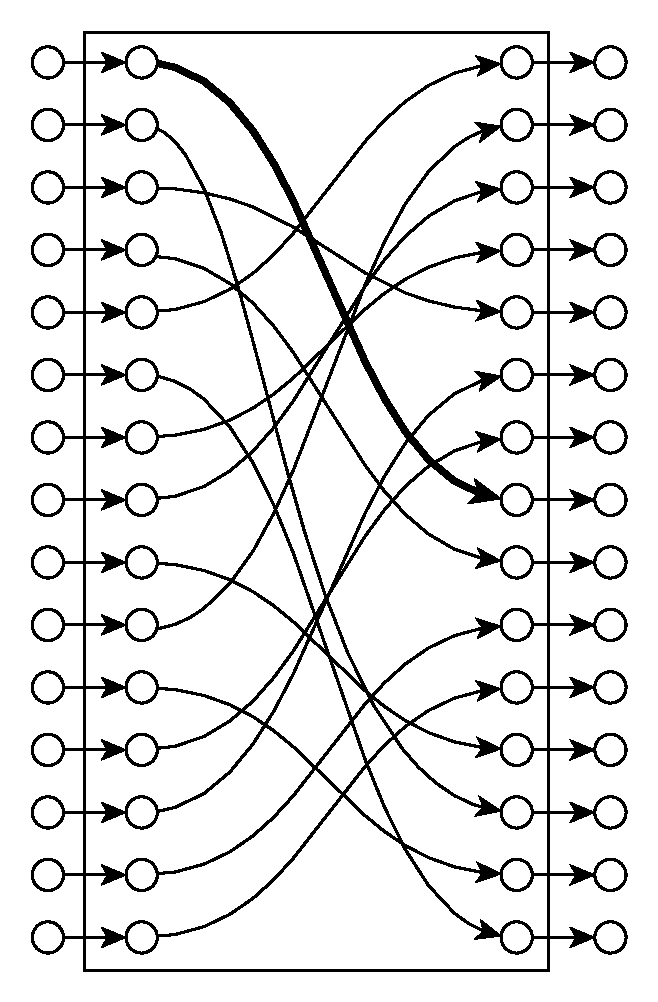
\includegraphics[width=0.25\textwidth]{pic/p-box-inside}}
		\caption{Возможные реализации s- и p-блоков}
\end{figure}

Фейстель высказал идею, что идеальный шифр для блока размером в 128 бит должен включать в себя блок замен (substitution box, s-box, далее s-блок), который мог бы обработать сразу 128 бит входного блока данных. S-блок принимает на вход блок битов и даёт на выходе другой блок бит (возможно, даже другого размера) согласно некоторому словарю или результату вычисления нелинейной функции\footnote{Нелинейная функция в целях производительности также может быть технологически реализована в виде выборки уже вычисленного значения по аргументу из словаря.}. К сожалению, физическая реализация (см. рис.~\ref{fig:s-box-inside}) действительно произвольного блока замен для входа в 128 бит потребовала бы $2^{128}$ внутренних соединений или словаря из $2^{128}$ 128-битовых значений, если реализовывать программным способом, что технологически невозможно\footnote{Причём в шифре таких блоков должно быть столько же, сколько разных ключей мог бы иметь шифр.}. Зато если такой блок можно было бы создать, то он был бы очень хорош с криптографической точки зрения. Даже если криптоаналитик знает произвольное число пар значений вход-выход, то это ничего не скажет ему об остальном множестве значений. То есть без полного перебора всех возможных $2^{128}$ вариантов входа криптоаналитик не сможет составить полное представление о внутренней структуре блока.

С другой стороны, блок перестановок (permutation box, p-box, далее p-блок), изображённый на рис.~\ref{fig:p-box-inside}, может обрабатывать блоки битов любого размера. Однако какая-либо криптографическая стойкость у него отсутствует: он представляет собой тривиальное линейное преобразование своего входа. Криптоаналитику достаточно иметь $N$ линейно независимых пар значений входа и выхода (где $N$ -- размер блока), чтобы получить полное представление о структуре p-блока.

\index{SP-сеть|(}
Идея Фейстеля состояла в том, чтобы комбинировать s- и p-блоки, позволяя на практике получить большой блок нелинейных преобразований (то есть один большой s-блок), как изображено на рис.~\ref{fig:sp-network}. При достаточном числе <<слоёв>> SP-сеть начинает обладать свойствами хорошего s-блока (сложностью криптографического анализа и выявления структуры), при этом оставаясь технологически простой в реализации.

\begin{figure}[htb]
	\centering
	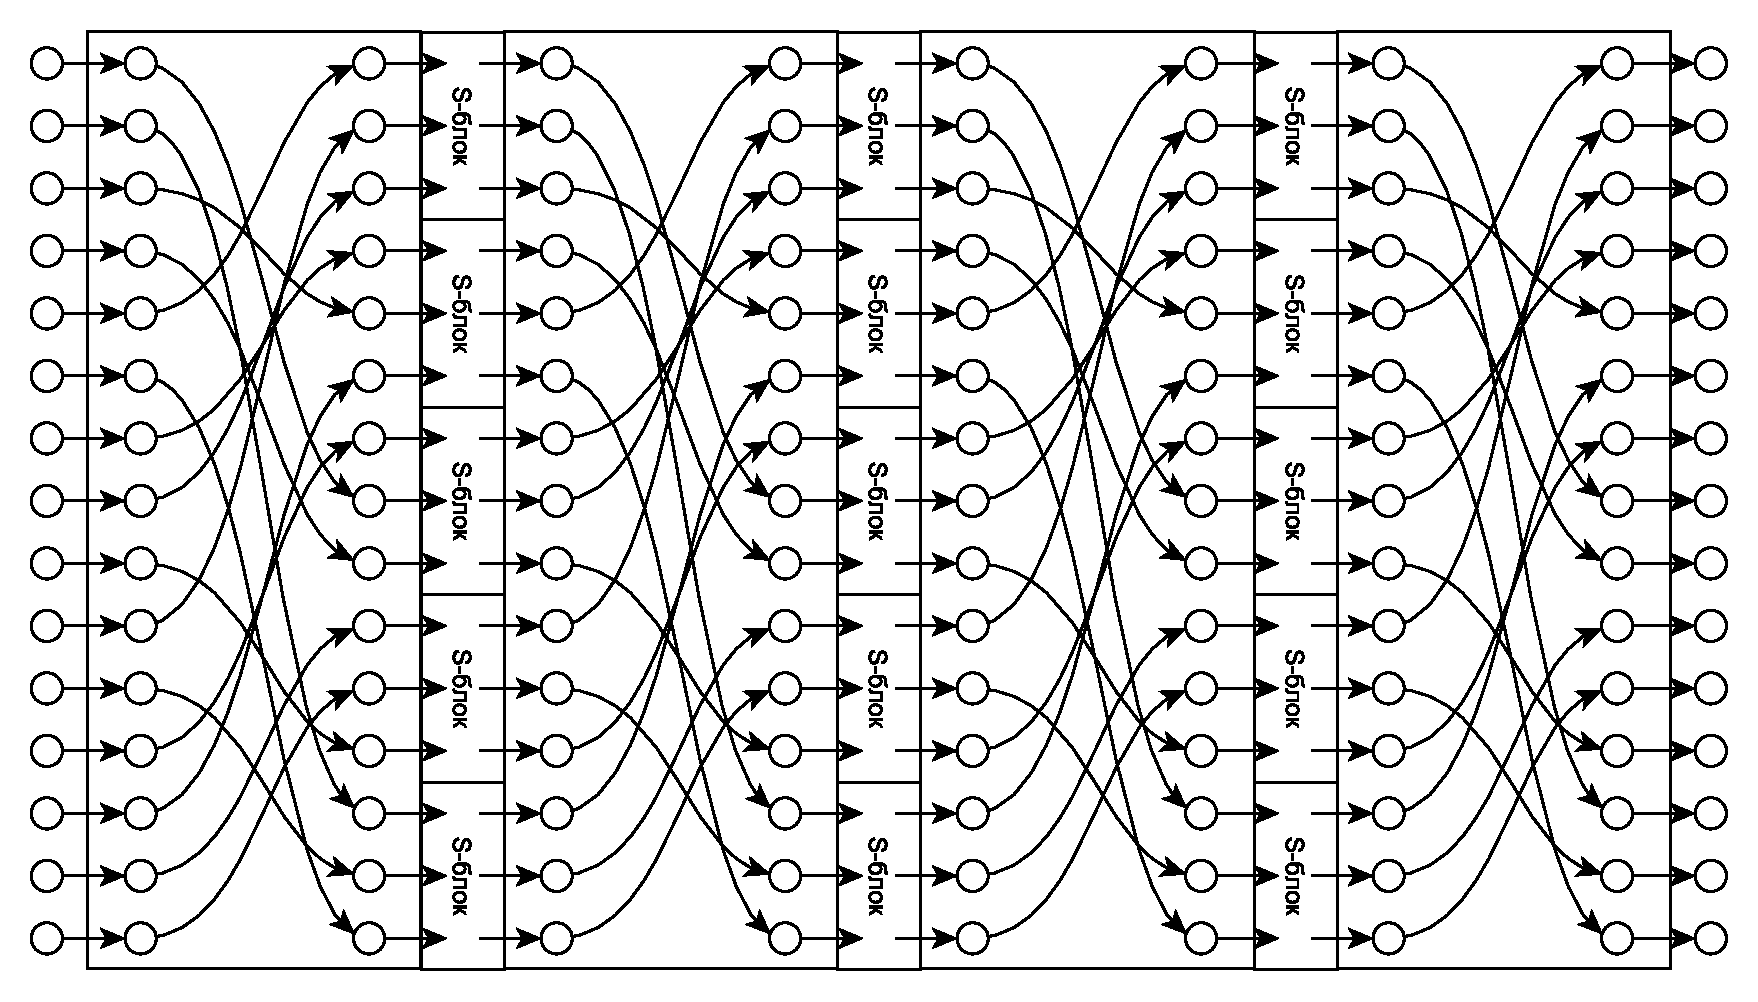
\includegraphics[width=0.8\textwidth]{pic/sp-network}
  \caption{SP-сеть, состоящая из 4 p-блоков и 3 слоёв s-блоков, по 5 блоков в каждом слое}
  \label{fig:sp-network}
\end{figure}

Следующей составляющей будущего шифра стала возможность менять используемые s-блоки в зависимости от ключа. Вместо каждого из s-блоков в SP-сети Фейстель поместил модуль с двумя разными s-блоками. В зависимости от одного из битов ключа (своего для каждой пары блоков) использовался первый или второй s-блок. Результатом данного подхода стал первый вариант шифра в проекте <<Люцифер>>, который в упрощённом виде (с меньшим размером блока и меньшим числом слоёв) изображён на рис.~\ref{fig:lucifer}.

\begin{figure}[htb]
	\centering
	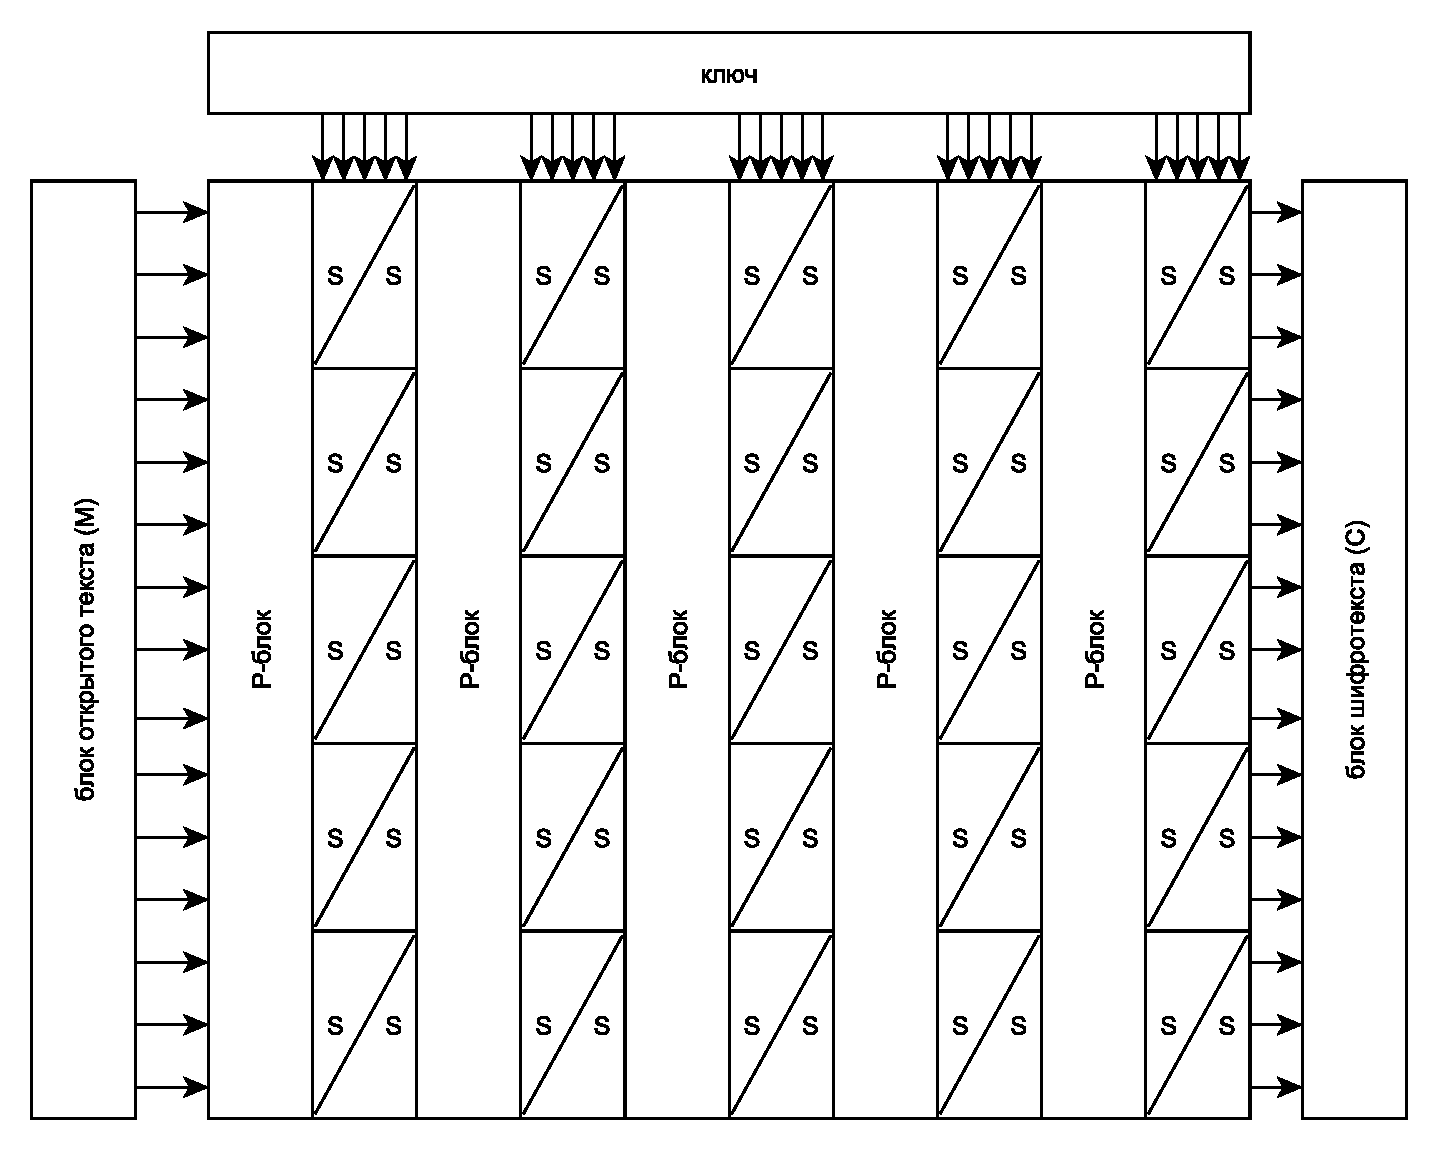
\includegraphics[width=0.8\textwidth]{pic/lucifer}
  \caption{Общий вид (упрощённая схема) функции шифрования в одном из вариантов проекта <<Люцифер>>. Входной блок (в проекте <<Люцифер>> его объём -- 128 бит) подавался на вход на несколько слоёв (в <<Люцифере>> слоёв 16) из p-блоков и пар s-блоков. S-блок в каждой паре выбирался в зависимости от значения соответствующего бита ключа}
  \label{fig:lucifer}
\end{figure}\index{SP-сеть|)}

Разделение функции шифрования на относительно простые раунды (<<слои>>), комбинация больших p-блоков со множеством s-блоков малого размера -- всё это до сих пор используется в современных блочных шифрах.

\index{шифр!Люцифер|)}


\section{Ячейка Фейстеля}\index{ячейка Фейстеля|(}
\selectlanguage{russian}

Следующей идеей, продвинувшей развитие блочных шифров и приведшей к появлению государственного стандарта DES\index{шифр!DES}, стала конструкция, получившая название \emph{ячейка Фейстеля}. Данная конструкция приведена на рис.~\ref{fig:Feistel}.

\begin{figure}[!htb]
    \centering
    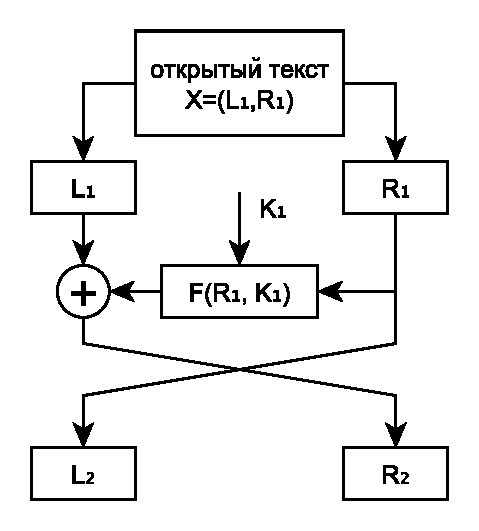
\includegraphics[width=0.6\textwidth]{pic/feistel}
    \caption{Ячейка Фейстеля\label{fig:Feistel}}
\end{figure}

На рис.~\ref{fig:Feistel} изображён один раунд шифрования блочного шифра, использующего оригинальную ячейку Фейстеля. Каждый раунд шифрования принимает на вход блок с чётным количеством бит и делит его на две равные части $L_k$ и $R_k$. Входным блоком для первого раунда является блок открытого текста. Правая часть $R_k$ без изменений становится левой частью входного блока $L_{k+1}$ следующего раунда шифрования. Кроме того, правая часть подаётся на вход \emph{функции Фейстеля} $F\left(R_k, K_k \right)$\index{функция!Фейстеля}, аргументами которой являются половина блока данных и раундовый ключ\index{ключ!раундовый} (раундовые ключи получаются в результате работы алгоритма ключевого расписания, как описано в разделе~\ref{section-block-ciphers-intro}). Результат работы функции Фейстеля складывается с помощью побитового сложения по модулю 2 с левой частью входного блока $L_k$. Полученная последовательность бит становится правой частью выходного блока раунда шифрования. Таким образом, работа $k$-го раунда ячейки Фейстеля описывается следующими соотношениями:
\[\begin{array}{l}
    L_{k+1} = R_{k}, \\
    R_{k+1} = L_{k} \oplus F\left( R_k, K_k \right).
\end{array}\]

Результатом шифрования является конкатенация последних выходных блоков $L_n$ и $R_n$, где $n$ -- число раундов шифрования.

Несложно показать, что зная раундовые ключи $K_1, \dots, K_n$ и результат шифрования $L_n$ и $R_n$, можно восстановить открытый текст. В частности, для каждого раунда:
\[\begin{array}{l}
    R_k = L_{k+1}, \\
    L_k = R_{k+1} \oplus F\left( R_k, K_k \right).
\end{array}\]

Таким образом, ячейка Фейстеля гарантирует корректность работы блочного шифра вне зависимости от сложности функции Фейстеля\index{функция!Фейстеля} $F\left(R_k, K_k \right)$. В результате криптограф (автор шифра) при использовании ячейки Фейстеля не должен беспокоиться об обратимости функции шифрования в целом (конструкция ячейки Фестеля уже гарантирует это), а должен беспокоиться только о достаточной криптографической стойкости функции Фейстеля, необратимость которой не требуется (и даже вредит криптостойкости). Функция Фейстеля обычно состоит из блоков перестановок и замен (то есть из p- и s-блоков, уже рассмотренных ранее).

\index{ячейка Фейстеля|)}


\section{Шифр DES}\index{шифр!DES|(}
\selectlanguage{russian}

Развитием проекта <<Люцифер>>\index{шифр!Люцифер} стал государственный стандарт США, известный как DES (\langen{data encryption standard}). Это первый из рассматриваемых нами блочных шифров, который имеет ярко выраженные раунды шифрования, отдельно выделенную функцию ключевого расписания и основан на классической ячейке Фейстеля\index{ячейка Фейстеля}. Поэтому для знакомства с шифром достаточно рассмотреть устройство функции Фейстеля\index{функция!Фейстеля} как основного элемента, отличающего данный шифр от аналогичных.

В шифре DES открытый текст делится на блоки по 32 бита, и они обрабатываются в 16 раундах. Раундовые ключи генерируются из исходных 64 бит ключа (при этом значащими являются только 56 бит, а последние 8 бит используются для проверки корректности ввода ключа). На вход функции Фейстеля для шифра DES, схема которой приведена на рис.~\ref{fig:des}, подаётся половина от размера входного блока -- 32 бита.

\begin{figure}[!htb]
    \centering
    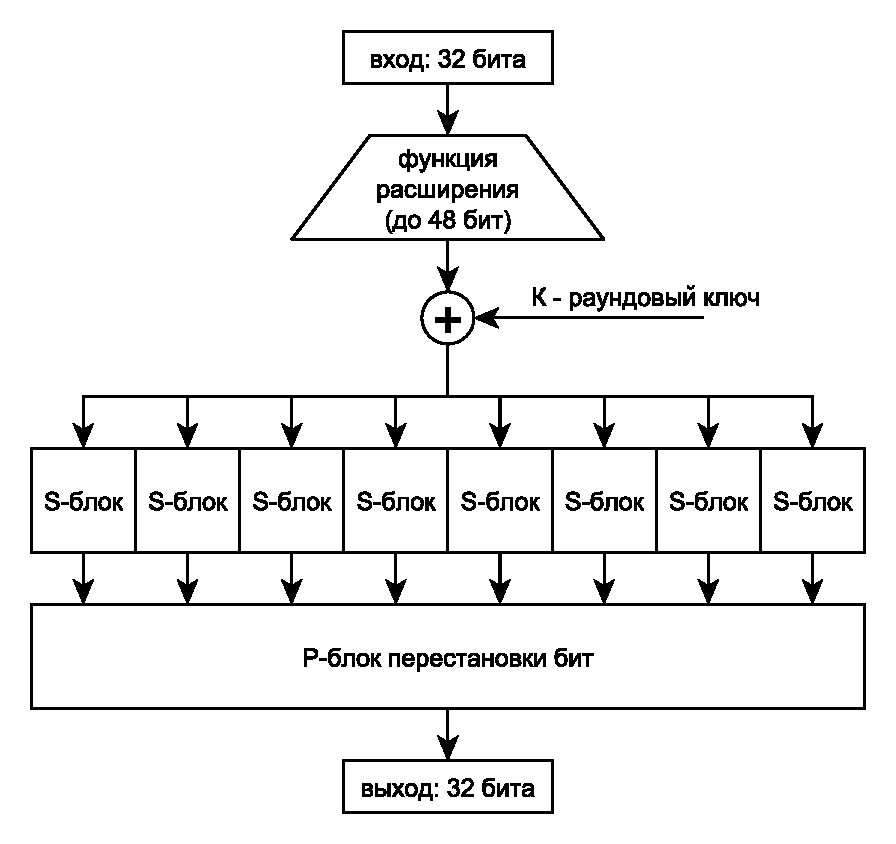
\includegraphics[width=0.75\textwidth]{pic/des}
    \caption{Функция Фейстеля\index{функция!Фейстеля} шифра DES\label{fig:des}}
\end{figure}

Эти 32 бита проходят через функцию расширения, которая с помощью дублирования отдельных битов превращает их в 48 бит. Они суммируются побитово по модулю 2 с раундовым ключом. Результат подаётся на вход 8 s-блоков, которые работают как таблицы замен последовательности из 6 бит в 4 бита (каждый блок). На выходе s-блоков получаются $8 \times 4 = 32$ бита, которые попадают в p-блок перестановки. Результат работы p-блока является результатом функции Фейстеля\index{функция!Фейстеля} для одного раунда шифра DES.

Интересно отметить, что изначально автором предполагалось использовать ключ в 128 бит, но под напором АНБ (Агентство национальной безопасности, \langen{National Security Agency, NSA}) он был сокращён до 56 бит, что на тот момент составляло вполне достаточную для криптостойкости величину. Кроме того, АНБ указало обязательные к использованию s-блоки (таблицы замен). Много позже, в 90-х годах, когда были разработаны методы линейного и дифференциального криптоанализа, выяснилось, что предложенные АНБ в 70-х годах s-блоки устойчивы к данным методам криптоанализа, как будто специально делались с учётом возможности их использования.

\index{шифр!DES|)}


\section{ГОСТ 28147-89}\index{шифр!ГОСТ 28147-89|(}
\selectlanguage{russian}

Российский стандарт шифрования, получивший известность как ГОСТ 28147-89 (\cite{GOST-89}), относится к действующим симметричным одноключевым криптографическим алгоритмам. Он зарегистрирован 2 июня 1989 года и введён в действие Постановлением Государственного комитета СССР по стандартам от 02.06.89 \No1409. В настоящий момент шифр известен под названиями <<ГОСТ>> (<<GOST>>) и <<Магма>>. Последнее название появилось в стандарте ГОСТ Р 34.12-2015~\cite{GOST-R:34.12-2015}, описывающем как данный блочный шифр, так и более новый шифр <<Кузнечик>>, о котором будет рассказано в разделе \ref{section-grig}.

ГОСТ 28147-89 устанавливает единый алгоритм криптографических преобразований для систем обмена информацией в вычислительных сетях и определяет правила шифрования и расшифрования данных, а также выработки имитовставки\index{имитовставка}. Основные параметры шифра таковы: размер блока составляет 64 бита, число раундов $m=32$, имеется 8 ключей по 32 бита каждый, так что общая длина ключа -- 256 бит. Основа алгоритма -- цепочка ячеек Фейстеля\index{ячейка Фейстеля}.

\begin{figure}[!ht]
    \centering
    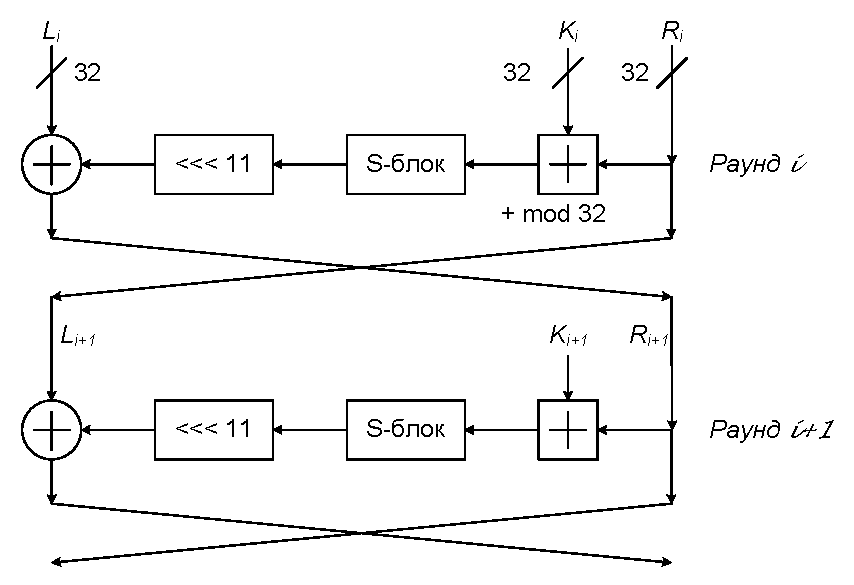
\includegraphics[width=0.6\textwidth]{pic/gost-28147-89}
    \caption{Схема ГОСТ 28147-89\label{fig:gost-28147-89}}
\end{figure}

Структурная схема алгоритма шифрования представлена на рис.~\ref{fig:gost-28147-89} и включает:
\begin{itemize}
    \item ключевое запоминающее устройство (КЗУ) на 256 бит, которое состоит из восьми 32-разрядных накопителей $(X_0, X_1, X_2, X_3, X_4, X_5, X_6, X_7)$ и содержит сеансовые ключи шифрования одного раунда;
    \item 32-разрядный сумматор $\boxplus$ по модулю $2^{32}$;
    \item сумматор $\oplus$ по модулю 2;
    \item блок подстановки $(S)$;
    \item регистр циклического сдвига на одиннадцать шагов в сторону старшего разряда $(R)$.
\end{itemize}

Блок подстановки $(S)$ состоит из 8 узлов замены -- s-блоков с памятью на 64 бита каждый. Поступающий на вход блока подстановки 32-разрядный вектор разбивается на 8 последовательных 4-разрядных векторов, каждый из которых преобразуется в 4-разрядный вектор соответствующим узлом замены. Узел замены представляет собой таблицу из 16 строк, содержащих по 4 бита в строке. Входной вектор определяет адрес строки в таблице, заполнение данной строки является выходным вектором. Затем 4-разрядные выходные векторы последовательно объединяются в 32-разрядный вектор.

При перезаписи информации содержимое $i$-го разряда одного накопителя переписывается в $i$-й разряд другого накопителя.

Ключ, определяющий заполнение КЗУ, и таблицы блока подстановки $K$ являются секретными элементами.

Стандарт не накладывает ограничений на степень секретности защищаемой информации.

ГОСТ 28147-89 удобен как для аппаратной, так и для программной реализаций.

Алгоритм имеет четыре режима работы:
\begin{itemize}
    \item простой замены,
    \item гаммирования,
    \item гаммирования с обратной связью,
    \item выработки имитовставки\index{имитовставка}.
\end{itemize}

Из них первые три -- режимы шифрования, а последний -- генерирования имитовставки\index{имитовставка} (другие названия: инициализирующий вектор, синхропосылка). Подробно данные режимы описаны в следующем разделе.

\index{шифр!ГОСТ 28147-89|)}


\section{Стандарт шифрования США AES}\index{шифр!AES|(}
\selectlanguage{russian}

До 2001 г. стандартом шифрования данных в США был DES\index{шифр!DES} (аббревиатура от Data Encryption Standard), который был принят в 1980 году. Входной блок открытого текста и выходной блок шифрованного текста DES составляли по 64 бита каждый, длина ключа -- 56 бит (до процедуры расширения). Алгоритм основан на ячейке Фейстеля\index{ячейка Фейстеля} с s-блоками и таблицами расширения и перестановки битов. Количество раундов -- 16.

Для повышения криптостойкости и замены стандарта DES был объявлен конкурс на новый стандарт AES (аббревиатура от Advanced Encryption Standard). Победителем конкурса стал шифр Rijndael. Название составлено с использованием первых слогов фамилий его создателей (Rijmen и Daemen). В русскоязычном варианте читается как <<Рэндал>>~\cite{Kiwi:1999}. 26 ноября 2001 года шифр был утверждён в качестве стандарта FIPS 197 и введён в действие 26 мая 2002 года~\cite{FIPS-PUB-197}.

AES -- это раундовый\index{шифр!раундовый} блочный\index{шифр!блочный} шифр с переменной длиной ключа (128, 192 или 256 бит) и фиксированными длинами входного и выходного блоков (128 бит).

\subsection[Состояние, ключ шифрования и число раундов]{Состояние, ключ шифрования и число \protect\\ раундов}

Различные преобразования воздействуют на результат промежуточного шифрования, называемый \emph{состоянием} ($\mathsf{State}$). Состояние представлено $(4 \times 4)$-матрицей из байтов $a_{i,j}$.

\emph{Ключ шифрования раунда} ($\mathsf{Key}$) также представляется прямоугольной $(4 \times \mathsf{Nk})$-матрицей из байтов $k_{i,j}$, где $\mathsf{Nk}$ равно длине ключа, разделённой на 32, то есть 4, 6 или 8.

Эти представления приведены ниже:
\[
    \mathsf{State} = \left[ \begin{array}{cccc}
        a_{0,0} & a_{0,1} & a_{0,2} & a_{0,3} \\
        a_{1,0} & a_{1,1} & a_{1,2} & a_{1,3} \\
        a_{2,0} & a_{2,1} & a_{2,2} & a_{2,3} \\
        a_{3,0} & a_{3,1} &a_{3,2} & a_{3,3}  \\
    \end{array} \right],
\] \[
    \mathsf{Key} = \left[ \begin{array}{cccc}
        k_{0,0} & k_{0,1} & k_{0,2} & k_{0,3} \\
        k_{1,0} & k_{1,1} & k_{1,2} & k_{1,3} \\
        k_{2,0} & k_{2,1} & k_{2,2} & k_{2,3} \\
        k_{3,0} & k_{3,1} & k_{3,2} & k_{3,3} \\
    \end{array} \right].
\]

Иногда блоки символов интерпретируются как одномерные последовательности из 4-байтных векторов, где каждый вектор является соответствующим столбцом прямоугольной таблицы. В этих случаях таблицы можно рассматривать как наборы из 4, 6 или 8 векторов, нумеруемых в диапазоне $0 \dots 3$, $0 \dots 5$ или $0 \dots 7$ соответственно. В тех случаях, когда нужно пометить индивидуальный байт внутри 4-байтного вектора, используется обозначение $(a, b, c, d)$, где $a$, $b$, $c$, $d$ соответствуют байтам в одной из позиций ($0$, $1$, $2$, $3$) в столбце или векторе.

\emph{Входные} и \emph{выходные} блоки шифра AES рассматриваются как последовательности 16 байтов $(a_0, a_1, \dots, a_{15})$. Преобразование входного блока $(a_0, \dots, a_{15})$ в исходную $(4 \times 4)$-матрицу состояния $\mathsf{State}$ или преобразование конечной матрицы состояния в выходную последовательность проводится по правилу (запись по столбцам):
    \[ a_{i,j} = a_{i + 4j}, ~ i = 0 \dots 3, ~ j = 0 \dots 3. \]

Аналогично ключ шифрования может рассматриваться как последовательность байтов $(k_0, k_1, \dots, k_{4 \cdot \mathsf{Nk} - 1})$, где $\mathsf{Nk} = 4, 6, 8$. Число байтов в этой последовательности равно 16, 24 или 32, а номера этих байтов находятся в интервалах $0 \dots 15$, $0 \dots 23$ или $0 \dots 31$ соответственно. $(4 \times \mathsf{Nk})$-матрица ключа шифрования $\mathsf{Key}$ задаётся по правилу:
    \[ k_{i,j} = k_{i + 4j}, ~ i = 0 \dots 3, ~ j = 0 \dots \mathsf{Nk} - 1. \]

Число раундов $\mathsf{Nr}$ зависит от длины ключа. Его значения приведены в таблице ниже.

\begin{center}
    \begin{tabular}{|l|c|c|c|}
    \hline
    Длина ключа, биты           &128 & 192 & 256 \\
    $\mathsf{Nk}$               & 4  & 6   & 8 \\
    Число раундов $\mathsf{Nr}$ & 10 & 12 & 14 \\
    \hline
    \end{tabular}
\end{center}


\subsection{Операции в поле}

При переходе от одного раунда к другому матрицы \emph{состояния} и \emph{ключа шифрования раунда} подвергаются ряду преобразований. Преобразования могут осуществляться над:
\begin{itemize}
    \item отдельными байтами или парами байтов (необходимо определить операции сложения и умножения);
    \item столбцами матрицы, которые рассматриваются как 4-мерные векторы с соответствующими байтами в качестве элементов;
    \item строками матрицы.
\end{itemize}

В алгоритме шифрования AES байты рассматриваются как элементы поля $\GF{2^8}$, а вектор-столбцы из четырёх байтов -- как многочлены третьей степени над полем $\GF{2^8}$. В приложении~\ref{chap:discrete-math} дано подробное описание этих операций.

Хотя определение операций дано через их математическое представление, в реализациях шифра AES активно используются таблицы с заранее вычисленными результатами операций над отдельными байтами, включая взятие обратного элемента и перемножение элементов в поле $\GF{2^8}$ (на что требуется 256 байт и 64 КиБ памяти соответственно).

\subsection{Операции одного раунда шифрования}

В каждом раунде шифра AES, кроме последнего, производятся следующие 4 операции:
\begin{itemize}
  \item замена байтов, $\mathsf{SubBytes}$;
  \item сдвиг строк, $\mathsf{ShiftRows}$;
  \item перемешивание столбцов, $\mathsf{MixColumns}$;
  \item добавление текущего ключа, $\mathsf{AddRoundKey}$.
\end{itemize}

В обозначениях, близких к языку С, можно записать программу в следующем виде:
\[
    \begin{array}{l}
        \mathsf{Round(State, RoundKey)} \{ \\
        ~~~~ \mathsf{SubBytes(State)}; \\
        ~~~~ \mathsf{ShiftRows(State)}; \\
        ~~~~ \mathsf{MixColumns(State)}; \\
        ~~~~ \mathsf{AddRoundKey(State, RoundKey)}; \\
        \} \\
    \end{array}
\]
В последнем раунде исключается операция <<перемешивание столбцов>>. Этот раунд можно записать в следующем виде:
\[
    \begin{array}{l}
        \mathsf{Round(State, RoundKey)} \{ \\
        ~~~~ \mathsf{SubBytes(State)}; \\
        ~~~~ \mathsf{ShiftRows(State)}; \\
        ~~~~ \mathsf{AddRoundKey(State, RoundKey)}; \\
        \} \\
    \end{array}
\]
В этих обозначениях все <<функции>>, а именно: $\mathsf{Round}$, $\mathsf{SubBytes}$, $\mathsf{ShiftRows}$, $\mathsf{MixColumns}$ и $\mathsf{AddRoundKey}$ воздействуют на матрицы, определяемые указателем $\mathsf{(State, RoundKey)}$. Сами преобразования описаны в следующих разделах.


\subsubsection{Замена байтов $\mathsf{SubBytes}$}

Нелинейная операция <<замена байтов>> действует независимо на каждый байт $a_{i,j}$ текущего состояния. Таблица замены (или s-блок) является обратимой и формируется последовательным применением двух преобразований.

\begin{enumerate}
    \item Сначала байт $a$ представляется как элемент $a(x)$ поля Галуа $\GF{2^8}$ и заменяется на обратный элемент $a^{-1} \equiv a^{-1}(x)$ в поле. Байт $\mathrm{'00'}$, для которого обратного элемента не существует, переходит сам в себя.
    \item Затем к обратному байту $a^{-1} = (x_0, x_1, x_2, x_3, x_4, x_5, x_6, x_7)$ применяется аффинное преобразование над полем $\GF{2^8}$ следующего вида:
        \[
            \left[  \begin{array}{c}
                y_{0} \\ y_{1} \\ y_{2} \\ y_{3} \\ y_{4} \\ y_{5} \\ y_{6} \\ y_{7} \\
            \end{array} \right] = \left[ \begin{array}{cccccccc}
                1 & 0 & 0  & 0 & 1 & 1 & 1 & 1 \\
                1 & 1 & 0  & 0 & 0 & 1 & 1 & 1 \\
                1 & 1 & 1  & 0 & 0 & 0 & 1 & 1 \\
                1 & 1 & 1  & 1 & 0 & 0 & 0 & 1 \\
                1 & 1 & 1  & 1 & 1 & 0 & 0 & 0 \\
                0 & 1 & 1  & 1 & 1 & 1 & 0 & 0 \\
                0 & 0 & 1  & 1 & 1 & 1 & 1 & 0 \\
                0 & 0 & 0  & 1 & 1 & 1 & 1 & 1  \
            \end{array} \right] \cdot \left[ \begin{array}{c}
                x_{0} \\ x_{1} \\ x_{2} \\ x_{3} \\ x_{4} \\ x_{5} \\ x_{6} \\ x_{7} \\
            \end{array} \right] + \left[ \begin{array}{c}
                1 \\ 1 \\ 0 \\ 0 \\ 0 \\ 1 \\ 1 \\ 0 \\
            \end{array} \right].
        \]
\end{enumerate}

В полиномиальном представлении это аффинное преобразование имеет вид
\[Y(z)=(z^4)X(z)(1+z+z^2+z^3+z^4)\mod(1+z^8) + F(z).\]
Применение описанных операций s-блока ко всем байтам текущего состояния обозначено
    \[ \mathsf{SubBytes(State)}. \]

Обращение операции $\mathsf{SubBytes(State)}$ также является заменой байтов. Сначала выполняется обратное аффинное преобразование, а затем от полученного байта берётся обратный.


\subsubsection{Сдвиг строк $\mathsf{ShiftRows}$}

Для выполнения операции <<сдвиг строк>> строки в таблице текущего состояния циклически сдвигаются влево. Величина сдвига различна для различных строк. Строка $0$ не сдвигается вообще. Строка $1$ сдвигается на $C_1=1$ позицию, строка $2$ -- на $C_2=2$ позиции, строка $3$ -- на $C_3=3$ позиции.
%Величины $C1,C2$ и $C3$ зависят от $Nb$. Их значения приведены в таблице~\ref{tab:AES-shift-rows}.
%
%\begin{table}[!ht]
%    \centering
%    \begin{tabular}{|c|c|c|c|}
%        \hline
%        Nb & C1 & C2 & C3 \\
%        \hline
%        4  & 1  & 2  & 3  \\
%        \hline
%        6  & 1  & 2  & 3  \\
%        \hline
%        8  & 1  & 3  & 4  \\
%        \hline
%    \end{tabular}
%    \caption{Сдвиг $C$ и длина блока $Nb$.}
%    \label{tab:AES-shift-rows}
%\end{table}


\subsubsection{Перемешивание столбцов $\mathsf{Mix Columns}$}

При выполнении операции <<перемешивание столбцов>> столбцы матрицы текущего состояния рассматриваются как многочлены над полем $\GF{2^8}$ и умножаются по модулю многочлена $y^4 +1$ на фиксированный многочлен $\mathbf{c}(y)$, где
    \[ \mathbf{c}(y) = \mathrm{'03'} y^3 + \mathrm{'01'} y^2 + \mathrm{'01'} y + \mathrm{'02'}. \]
Этот многочлен взаимно прост с многочленом $y^4 + 1$ и, следовательно, обратим. Перемножение удобнее проводить в матричном виде. Если $\mathbf{b}(y) = \mathbf{c}(y) \otimes \mathbf{a}(y)$, то
\[
    \left[ \begin{array}{c}
        b_{0} \\ b_{1} \\ b_{2} \\ b_{3} \\
    \end{array}\right] =  \left[ \begin{array}{cccc}
        \mathrm{'02'} & \mathrm{'03'} & \mathrm{'01'} & \mathrm{'01'} \\
        \mathrm{'01'} & \mathrm{'02'} & \mathrm{'03'} & \mathrm{'01'} \\
        \mathrm{'01'} & \mathrm{'01'} & \mathrm{'02'} & \mathrm{'03'} \\
        \mathrm{'03'} & \mathrm{'01'} & \mathrm{'01'} & \mathrm{'02'} \\
    \end{array} \right] \cdot \left[ \begin{array}{c}
        a_{0} \\ a_{1} \\ a_{2} \\ a_{3} \\
     \end{array} \right].
\]

Обратная операция состоит в умножении на многочлен $\mathbf{d}(y)$, обратный многочлену $\mathbf{c}(y)$ по модулю $y^4 + 1$, то есть
\[
    (\mathrm{'03'} y^{3} + \mathrm{'01'} y^{2} + \mathrm{'01'} y + \mathrm{'02'}) \otimes \mathbf{d}(y) = \mathrm{'01'}.
\]
Этот многочлен равен
\[
    \mathbf{d}(y) = \mathrm{'0B'} y^3 + \mathrm{'0D'} y^2 + \mathrm{'09'} y + \mathrm{'0E'}.
\]


\subsubsection{Добавление ключа раунда $\mathsf{AddRoundKey}$}

Операция <<добавление ключа раунда>> состоит в том, что матрица текущего состояния складывается по модулю 2 с матрицей ключа текущего раунда. Обе матрицы должны иметь одинаковые размеры. Матрица ключа раунда вычисляется с помощью процедуры \emph{расширения ключа}, описанной ниже. Операция <<добавление ключа раунда>> обозначается $\mathsf{AddRoundKey(State, RoundKey)}$.

\begin{multline*}
    \left[ \begin{array}{cccc}
        a_{0,0} & a_{0,1} & a_{0,2} & a_{0,3} \\
        a_{1,0} & a_{1,1} & a_{1,2} & a_{1,3} \\
        a_{2,0} & a_{2,1} & a_{2,2} & a_{2,3} \\
        a_{3,0} & a_{3,1} & a_{3,2} & a_{3,3}
    \end{array} \right]
    \oplus
    \left[ \begin{array}{cccc}
        k_{0,0} & k_{0,1} & k_{0,2} & k_{0,3} \\
        k_{1,0} & k_{1,1} & k_{1,2} & k_{1,3} \\
        k_{2,0} & k_{2,1} & k_{2,2} & k_{2,3} \\
        k_{3,0} & k_{3,1} & k_{3,2} & k_{3,3}
    \end{array} \right] =
    \\
    = \left[ \begin{array}{cccc}
        b_{0,0} & b_{0,1} & b_{0,2} & b_{0,3} \\
        b_{1,0} & b_{1,1} & b_{1,2} & b_{1,3} \\
        b_{2,0} & b_{2,1} & b_{2,2} & b_{2,3} \\
        b_{3,0} & b_{3,1} & b_{3,2} & b_{3,3}
    \end{array} \right].
\end{multline*}


\subsection{Процедура расширения ключа}

Матрица ключа текущего раунда вычисляется из исходного ключа шифра с помощью специальной процедуры, состоящей из расширения ключа и выбора раундового ключа. Основные принципы этой процедуры состоят в следующем:
\begin{itemize}
    \item суммарная длина ключей всех раундов равна длине блока, умноженной на увеличенное на 1 число раундов. Для блока длины 128 бит и 10 раундов общая длина всех ключей раундов равна 1408;
    \item с помощью ключа шифра находят \emph{расширенный ключ};
    \item ключи \emph{раунда} выбираются из \emph{расширенного} ключа по правилу: ключ первого раунда состоит из первых 4 столбцов матрицы расширенного ключа, второй ключ -- из следующих 4 столбцов и~т.\,д.
\end{itemize}

Расширенный ключ -- это матрица $\mathsf{W}$, состоящая из $4(\mathsf{Nr} + 1)$ 4-байтных вектор-столбцов, каждый столбец $i$ обозначается $\mathsf{W}[i]$.

Далее рассматривается только случай, когда ключ шифра состоит из 16 байтов. Первые $\mathsf{Nk} = 4$ столбца содержат ключ шифра. Остальные столбцы вычисляются рекурсивно из столбцов с меньшими номерами.

Для $\mathsf{Nk} = 4$ имеем 16-байтный ключ
\[
    \mathsf{Key} = (\mathsf{Key}[0], \mathsf{Key}[1], \dots, \mathsf{Key}[15]).
\]
Приведём алгоритм расширения ключа для $\mathsf{Nk} = 4$.
\begin{algorithm}[ht]
    \caption{$\mathsf{KeyExpansion}(\mathsf{Key}, \mathsf{W})$\label{alg:AES-key-exp}}
    \begin{algorithmic}
        \FOR{ $i=0$ \TO $\mathsf{Nk} - 1$}
            \STATE $\mathsf{W}[i] = (\mathsf{Key}[4i], ~ \mathsf{Key}[4i+1], ~ \mathsf{Key}[4i+2], ~ \mathsf{Key}[4i+3])^T$;
        \ENDFOR
        \FOR{ $i = \mathsf{Nk}$ \TO $4(\mathsf{Nr} + 1) - 1$}
            \STATE $\mathsf{temp} = \mathsf{W}[i-1]$;
            \IF{ ($i = 0 \mod \mathsf{Nk}$)}
                \STATE $\mathsf{temp} = \mathsf{SubWord}(\mathsf{RotWord}(\mathsf{temp})) ~ \oplus ~ \mathsf{Rcon}[i ~/~ \mathsf{Nk}]$;
            \ENDIF
            \STATE $\mathsf{W}[i] = \mathsf{W}[i - \mathsf{Nk}] ~ \oplus ~ \mathsf{temp}$;
        \ENDFOR
    \end{algorithmic}
\end{algorithm}

%\[
%    \begin{array}{l}
%        \mathsf{KeyExpansion}(\mathsf{Key}, \mathsf{W}) \{ \\
%        ~~~~ \mathsf{for ~ (i = 0; ~ i < Nk = 4; ~ i++)} \\
%        ~~~~~~~~ \mathsf{W[i] = (Key[4 \cdot i], ~ Key[4*i+1], ~ Key[4*i+2], ~ Key[4*i+3]);} \\
%        ~~~~ \mathsf{for ~ (i = Nk; ~ i < 4 * (Nr + 1); ~ i++)} ~ \{ \\
%        ~~~~~~~~ \mathsf{temp = W[i-1];} \\
%        ~~~~~~~~ \mathsf{if ~ (i ~ \% ~ Nk ~ == ~ 0)} \\
%        ~~~~~~~~~~~~ \mathsf{temp = SubWord(RotWord(temp))} ~ \oplus ~ \mathsf{Rcon[i / Nk];} \\
%        ~~~~~~~~ \mathsf{W[i] = W[i - Nk]} ~ \oplus ~ \mathsf{temp;} \\
%        ~~~~ \} \\
%        \} \\
%    \end{array}
%\]

Здесь $\mathsf{SubWord}(\mathsf{W}[i])$ обозначает функцию, которая применяет операцию <<замена байтов>> (или s-блок) $\mathsf{SubBytes}$ к каждому из 4 байтов столбца $\mathsf{W}[i]$. Функция $\mathsf{RotWord}(\mathsf{W}[i])$ осуществляет циклический сдвиг вверх байт столбца $\mathsf{W}[i]$: если $\mathsf{W}[i] = (a, b, c, d)^T$, то $\mathsf{RotWord}(\mathsf{W}[i]) = (b, c, d, a)^T$. Векторы-константы $\mathsf{Rcon}[i]$ определены ниже.

Как видно из этого описания, первые $\mathsf{Nk} = 4$ столбца заполняются ключом шифра. Все следующие столбцы $\mathsf{W}[i]$ равны сумме по модулю $2$ предыдущего столбца $\mathsf{W}[i-1]$ и столбца $\mathsf{W}[i-4]$. Для столбцов $\mathsf{W}[i]$ с номерами $i$, кратными $\mathsf{Nk} = 4$, к столбцу $\mathsf{W}[i-1]$ применяются операции $\mathsf{RotWord(W)}$ и $\mathsf{SubWord(W)}$, а затем производится суммирование по модулю 2 со столбцом $\mathsf{W}[i-4]$ и константой раунда $\mathsf{Rcon}[i ~/~ 4]$.

%Для $\mathsf{Nk}>6$ имеем
%\[
%\begin{array}{l}
% \mathsf{KeyExpansion\,(byte\,Key\,[4*Nk]\,\, word \,\, W[Nb*(Nr+1)])}\\
%  \{\\
% \quad\quad \mathsf{for\,\,(i=0;\,\, i<Nk;\,\,i++)} \\
%  \qquad \quad\quad\quad \mathsf{W[i]=(Key[4*i];Key[4*i+1];Key[4*i+2];Key[4*i+3]);}\\
%  \quad\quad \mathsf{for \,\,(i=Nk;\,\,i<Nb*(Nr+1);\,\,i++)}\\
%  \quad\quad \{ \\
%  \quad \quad\quad\quad \mathsf{temp=W[i-1]}; \\
%  \quad \quad\quad\quad \mathsf{if\,\,(i\quad\% \quad Nk==0)}\\
%  \qquad \qquad \qquad \quad \mathsf{temp=SubByte(RotByte(temp))\quad\widehat{\,}\quad Rcon[i/Nk]};\\
%\quad \quad\quad\quad \mathsf{else \,\,if\,\,(i\quad\% \quad Nk==4)}\\
% \qquad \qquad \qquad \quad \mathsf{temp=SubByte(temp)};\\
%  \quad \quad\quad\quad \mathsf{W[i]=W[i-Nk] \quad\widehat{\,}\quad temp};\\
%  \quad\quad \} \\
%  \}\, \\
%\end{array}
%\]
%Различие между этими двумя случаями состоит в том, что во втором случае к столбцу $\mathsf{W[i-1]}$ применяются операции
% $\mathsf{RotByte(W)}$ и $\mathsf{SubByte(W)}$, если $\mathsf{i-4}$ кратно $\mathsf{Nk}$.\\

Векторы-константы раундов определяются следующим образом:
    \[ \mathsf{Rcon}[i] = (\mathsf{RC}[i], \mathrm{'00'}, \mathrm{'00'}, \mathrm{'00'})^T, \]
где байт $\mathsf{RC}[1] = \mathrm{'01'}$, а байты $\mathsf{RC}[i] = \alpha^{i-1}, ~ i = 2, 3, \dots$; байт $\alpha = \mathrm{'02'}$ -- это примитивный элемент поля $\GF{2^8}$.

\example
Пусть $\mathsf{Nk} = 4$. В этом случае ключ шифра имеет длину 128 бит. Найдём столбцы расширенного ключа. Столбцы $\mathsf{W}[0], \mathsf{W}[1], \mathsf{W}[2], \mathsf{W}[3]$ непосредственно заполняются битами ключа шифра. Номер следующего столбца $\mathsf{W}[4]$ кратен $\mathsf{Nk}$, поэтому
\[
    \mathsf{W}[4] = \mathsf{SubWord}(\mathsf{RotWord}(\mathsf{W}[3])) \oplus \mathsf{W}[0] \oplus
        \left[ \begin{array}{c}
            \mathrm{'01'} \\ \mathrm{'00'} \\ \mathrm{'00'} \\ \mathrm{'00'} \\
        \end{array} \right].
\]
Далее имеем:
\[
    \begin{array}{l}
        \mathsf{W}[5] = \mathsf{W}[4] \oplus \mathsf{W}[1], \\
        \mathsf{W}[6] = \mathsf{W}[5] \oplus \mathsf{W}[2], \\
        \mathsf{W}[7] = \mathsf{W}[6] \oplus \mathsf{W}[3].  \\
    \end{array}
\]
Затем:
\[
    \mathsf{W}[8] = \mathsf{SubWord}(\mathsf{RotWord}(\mathsf{W}[7])) \oplus \mathsf{W}[4] \oplus
        \left[ \begin{array}{c}
            \alpha \\
            \mathrm{'00'}\\
            \mathrm{'00'}\\
            \mathrm{'00'}\\
        \end{array} \right] ,
\] \[
    \begin{array}{l}
        \mathsf{W}[9] = \mathsf{W}[8] \oplus \mathsf{W}[5], \\
        \mathsf{W}[10] = \mathsf{W}[9] \oplus \mathsf{W}[6], \\
        \mathsf{W}[11] = \mathsf{W}[10] \oplus \mathsf{W}[7] \\
    \end{array}
\]
и~т.\,д.
\exampleend

%\example
%Пусть $\mathsf{Nk=6}.$ В этом случае ключ шифра имеет длину 192 бита. Найдём столбцы расширенного ключа. Столбцы $\mathsf{W[0],W[1],W[2],W[3],W[4],W[5]}$ непосредственно заполняются
%битами ключа шифра. Номер следующего столбца $\mathsf{W[6]}$ кратен $\mathsf{Nk}$, поэтому
%\[
%\begin{array}{ccccccc}
% \mathsf{W[6]} & = & \mathsf{SubByte(RotByte(W[5]))} &\oplus  &  \mathsf{W[0]} & \oplus  & \left[ \begin{array}{c}
% \mathsf{`01'} \\
%  \mathsf{`00'}\\
%  \mathsf{`00'}\\
%  \mathsf{`00'}\\
%\end{array}
%\right]    \\
%\end{array}
%\].
%
%Далее имеем
%\[
%\begin{array}{ccc}
% \mathsf{W[7]=W[6]}\oplus \mathsf{W[1]}; & \mathsf{W[8]=W[7]}\oplus \mathsf{W[2]}; & \mathsf{W[9]=W[8]}\oplus \mathsf{W[3]}; \\
% \mathsf{W[10]=W[9]}\oplus \mathsf{W[4]}; &\mathsf{ W[11]=W[10]}\oplus \mathsf{W[5]}.\\
%\end{array}
%\]
%Затем
%\[
%\begin{array}{ccccccc}
% \mathsf{W[12]} & = & \mathsf{SubByte(RotByte(W[11]))} &\oplus  &  \mathsf{W[6]} & \oplus  & \left[ \begin{array}{c}
% \mathsf{\alpha} \\
%  \mathsf{`00'}\\
%  \mathsf{`00'}\\
%  \mathsf{`00'}\\
%\end{array}
%\right] , \\
%\end{array}
%\]
%\[
%\begin{array}{ccc}
% \mathsf{W[13]=W[12]}\oplus \mathsf{W[7]}; & \mathsf{W[14]= W[13]}\oplus \mathsf{W[8]};  & \mathsf{W[15]=W[14]}\oplus \mathsf{W[9]}, \\
%\end{array}
%\]
%и~т.\,д.
%\exampleend
%
%\example
%Пусть $\mathsf{Nk=8}.$ В этом случае ключ шифра имеет длину $256$ бита. Найдём столбцы расширенного ключа. Столбцы
%$\mathsf{W[0],W[1],W[2],W[3],W[4],W[5],W[6],W[7]}$ непосредственно заполняются битами ключа шифра. Номер следующего столбца
%$\mathsf{W[8]}$ кратен $\mathsf{Nk}$, поэтому
%\[
%\begin{array}{ccccccc}
% \mathsf{W[8]} & = & \mathsf{SubByte(RotByte(W[7]))} &\oplus  &  \mathsf{W[0]} & \oplus  & \left[ \begin{array}{c}
% \mathsf{`01'} \\
%  \mathsf{`00'}\\
%  \mathsf{`00'}\\
%  \mathsf{`00'}\\
%\end{array}
%\right]    \\
%\end{array}
%\].
%Далее имеем
%\[
%\begin{array}{ccc}
%\mathsf{ W[7]=W[6]}\oplus \mathsf{W[1]}; & \mathsf{W[8]=W[7]}\oplus \mathsf{W[2]}; & \mathsf{W[9]=W[8]}\oplus \mathsf{W[3]}; \\
%\mathsf{ W[10]=W[9]}\oplus \mathsf{W[4]}; & \mathsf{W[11]=W[10]}\oplus \mathsf{W[5]}.\\
%\end{array}
%\]
%Номер следующего столбца $\mathsf{W[12]}$ равен $12$. Так как $12-4$ кратно $\mathsf{Nk}$, то
%\[
%\begin{array}{ccc}
%\mathsf{ W[12]=SubByte(RotByte(W[11]))}\oplus \mathsf{W[4]}; & \mathsf{W[13]=W[12]}\oplus \mathsf{W[5]}; & \mathsf{W[14]=W[13]}\oplus \mathsf{W[6]}; \\
%\mathsf{ W[15]=W[14]}\oplus \mathsf{W[7]}. &  &\\
%\end{array}
%\]
%Затем
%\[
%\begin{array}{ccccccc}
% \mathsf{W[16]} & = & \mathsf{SubByte(RotByte(W[15]))} &\oplus  &  \mathsf{W[8]} & \oplus  & \left[ \begin{array}{c}
% \mathsf{\alpha} \\
%  \mathsf{`00'}\\
%  \mathsf{`00'}\\
%  \mathsf{`00'}\\
%\end{array}
%\right] , \\
%\end{array}
%\]
%\[
%\begin{array}{ccc}
% \mathsf{W[17]=W[16]}\oplus \mathsf{W[9]}; & \mathsf{W[18]=W[17]}\oplus \mathsf{W[10]};  &\mathsf{ W[19]=W[18]}\oplus \mathsf{W[10]}, \\
%\end{array}
%\]
%
%\[
%\begin{array}{ccc}
%\mathsf{ W[20]=SubByte(RotByte(W[19]))}\oplus \mathsf{W[12]}; & \mathsf{W[21]=W[20]}\oplus \mathsf{W[13]}; & \mathsf{W[22]=W[21]}\oplus \mathsf{W[14]}; \\
%\mathsf{ W[23]=W[22]}\oplus \mathsf{W[15]}, &  &\\
%\end{array}
%\]
%и~т.\,д.

Ключ $i$-го раунда состоит из столбцов матрицы расширенного ключа
\[
    \mathsf{RoundKey} = (\mathsf{W}[4(i-1)], \mathsf{W}[4(i-1) + 1], \ldots, \mathsf{W}[4i-1]).
\]
%Если длина блока равна 192 битам $Nb=6$, то ключ 5-го раунда состоит из столбцов $W[24],W[25],W[26],W[27],W[28],W[29].$
%\exampleend

В настоящее время американский стандарт шифрования AES де-факто используется во всём мире в негосударственных системах передачи данных, если позволяет законодательство страны. C 2010 года процессоры Intel поддерживают специальный набор инструкций для шифра AES.

\index{шифр!AES|)}


\section{Шифр «Кузнечик»}\label{section-grig}\index{шифр!Кузнечик|(}
\selectlanguage{russian}

В июне 2015 года в России был принят новый стандарт блочного шифрования ГОСТ Р 34.12-2015~\cite{GOST-R:34.12-2015}. Данный стандарт включает в себя два блочных шифра -- старый ГОСТ 28147-89, получивший теперь название <<Магма>>, и новый шифр со 128-битным входным блоком, получившим название <<Кузнечик>>.

В отличие от шифра <<Магма>>, новый шифр <<Кузнечик>> основан на SP-сети\index{SP-сеть} (сети замен и перестановок), то есть основан на серии обратимых преобразований, а не на ячейке Фейстеля\index{ячейка Фейстеля}. Как и другие популярные шифры, он является блочным раундовым шифром и имеет выделенную процедуру выработки раундовых ключей. Шифр работает с блоками открытого текста по 128 бит, а размер ключа шифра составляет 256 бит. Отдельный раунд шифра <<Кузнечик>> состоит из операции наложения ключа, нелинейного и линейного преобразований, как изображено на рис.~\ref{fig:kuznechik-step}. Всего в алгоритме 10 раундов, последний из которых состоит только из операции наложения ключа. 

\begin{figure}[htb]
	\centering
	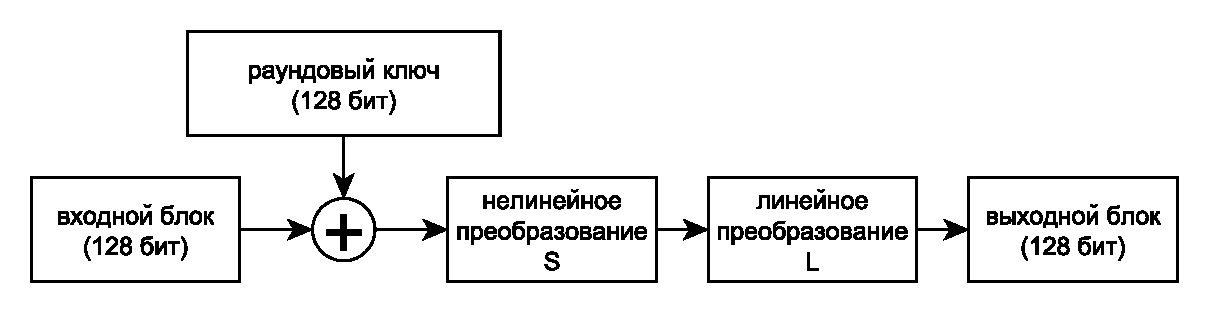
\includegraphics[width=0.8\textwidth]{pic/kuznechik-step}
  \caption{Один раунд шифрования в алгоритме <<Кузнечик>>}
  \label{fig:kuznechik-step}
\end{figure}

Нелинейное преобразование $S$ разбивает блок данных из 128 бит на 16 блоков по 8 бит в каждом, как показано на рис.~\ref{fig:kuznechik-s}.

\begin{figure}[htb]
	\centering
	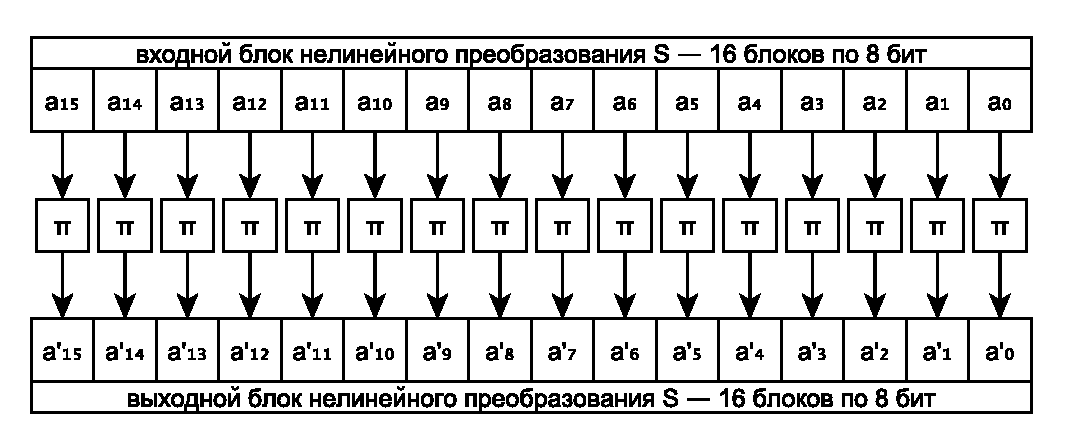
\includegraphics[width=0.9\textwidth]{pic/kuznechik-s}
  \caption{Нелинейное преобразование $S$ в алгоритме <<Кузнечик>>}
  \label{fig:kuznechik-s}
\end{figure}

Каждый из 16 восьмибитных блоков $a$ трактуется как целое беззнаковое число $\text{Int}_8 a$ и выступает в качестве индекса в заданном массиве констант $\pi'$. Значение по индексу $\text{Int}_8 a$ в массиве констант $\pi'$ обратно преобразуется в двоичный вид и выступает в качестве одного из 16 выходных блоков нелинейного преобразования $S$.

\begin{quote}\noindent {\scriptsize$\pi'$ = (252, 238, 221, 17, 207, 110, 49, 22, 251, 196, 250, 218, 35, 197, 4, 77, 233, 119, 240, 219, 147, 46, 153, 186, 23, 54, 241. 187, 20, 205, 95, 193, 249, 24, 101, 90, 226, 92, 239, 33, 129, 28, 60, 66, 139, 1, 142, 79, 5, 132, 2, 174, 227, 106, 143, 160, 6, 11, 237, 152, 127, 212, 211, 31, 235, 52, 44, 81, 234, 200, 72, 171, 242, 42, 104, 162, 253, 58, 206, 204, 181, 112, 14, 86, 8, 12, 118, 18, 191, 114, 19, 71, 156, 183, 93, 135, 21, 161, 150, 41, 16, 123, 154, 199, 243, 145, 120, 111, 157, 158, 178, 177, 50, 117, 25, 61, 255, 53, 138, 126, 109, 84, 198, 128, 195, 189, 13, 87, 223, 245, 36, 169, 62, 168, 67, 201, 215, 121, 214, 246, 124, 34, 185, 3, 224, 15, 236, 222, 122, 148, 176, 188, 220, 232, 40, 80, 78, 51, 10, 74, 167, 151, 96, 115, 30, 0, 98, 68, 26, 184, 56, 130, 100, 159, 38, 65, 173, 69, 70, 146, 39, 94, 85, 47, 140, 163, 165, 125, 105, 213, 149, 59, 7, 88, 179, 64, 134, 172, 29, 247, 48, 55, 107, 228, 136, 217, 231, 137, 225, 27, 131, 73, 76, 63, 248, 254, 141, 83, 170, 144, 202, 216, 133, 97, 32, 113, 103, 164, 45, 43, 9, 91, 203, 155, 37, 208, 190, 229, 108, 82, 89, 166, 116, 210, 230, 244, 180, 192, 209, 102, 175, 194, 57, 75, 99, 182).}\end{quote}

Линейное преобразование $L$ состоит из 16 операций линейного преобразования $R$, то есть $L = R^{16}$. Линейное преобразование $R$, в свою очередь, использует блок из 128 бит как начальные значения 8 битовых ячеек регистра сдвига, связанного с 16 ячейками линейной обратной связью (РСЛОС), как показано на рис.~\ref{fig:kuznechik-p}. При сдвиге вычисляется сумма значений ячеек, домноженных на 16 констант. Значения ячеек и константы трактуются как элементы поля Галуа $GF(2^8)$ с модулем $p(x) = x^8 + x^7 + x^6 + x + 1$ (см. раздел~\ref{section-fields}), умножение и сложение также проходят в этом поле.

\begin{figure}[htb]
	\centering
	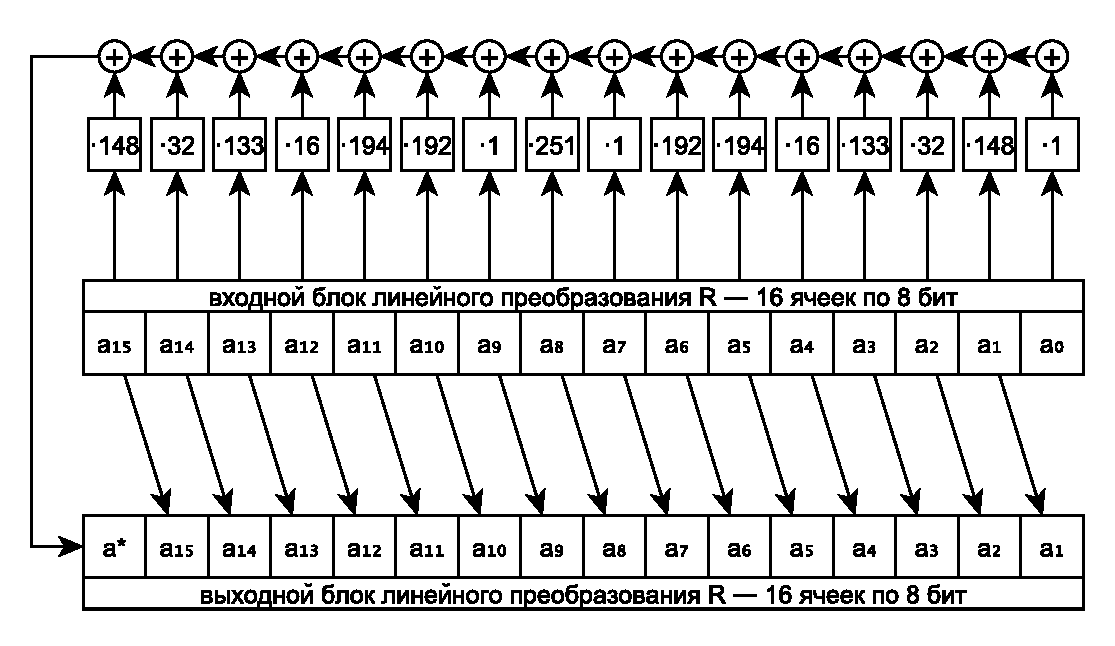
\includegraphics[width=0.9\textwidth]{pic/kuznechik-p}
  \caption{Линейное преобразование $R$ в алгоритме <<Кузнечик>>}
  \label{fig:kuznechik-p}
\end{figure}

Алгоритм развёртывания ключа основан на ячейке Фейстеля, хотя и не использует её ключевую особенность -- обратимость. Начало алгоритма изображено на рис.~\ref{fig:kuznechik-keys}.

\begin{figure}[htb]
	\centering
	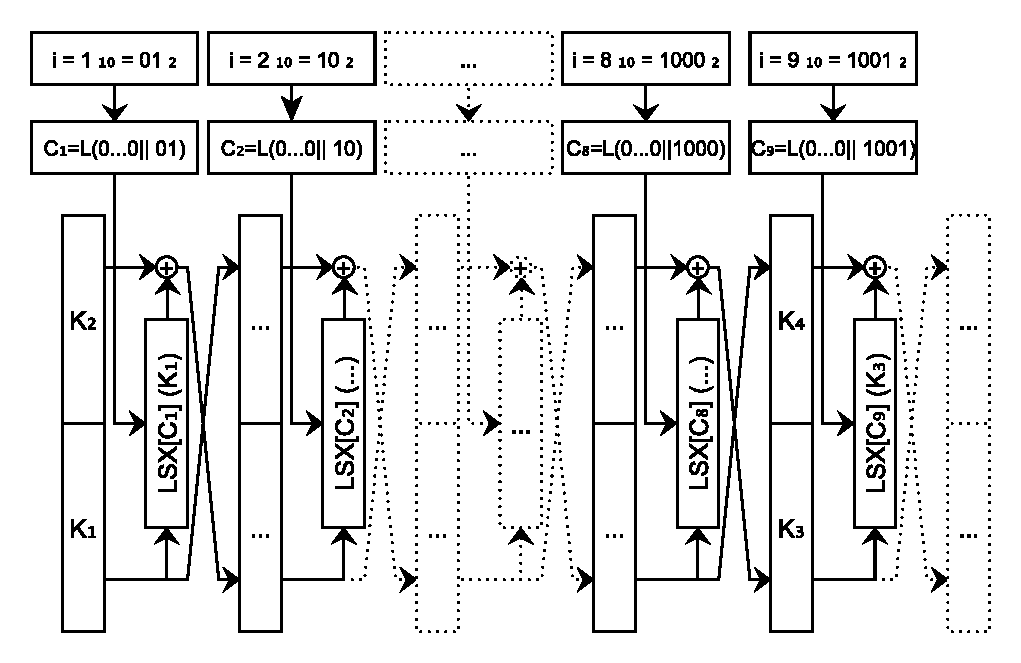
\includegraphics[width=0.90\textwidth]{pic/kuznechik-keys}
  \caption{Часть алгоритма развёртывания ключа в <<Кузнечике>>}
  \label{fig:kuznechik-keys}
\end{figure}

\begin{itemize}
	\item Целые числа $i$ от 1 до 32 представляются в виде двоичных векторов по 128 бит. К каждому из них применяется линейное преобразование $L=R^{16}$, как было описано ранее. Получаются 32 константы $C_{1}, \dots, C_{32}$.
	\item Первые два раундовых ключа $K_1$ и $K_2$ получаются разбиением мастер-ключа $K$ (256 бит) на два блока по 128 бит каждый.
	\item Следующая пара раундовых ключей $K_3$ и $K_4$ получается из первой пары $K_1$ и $K_2$ применением 8 раундов ячейки Фейстеля. В качестве функции Фейстеля, преобразующей один из блоков на каждом раунде, выступает преобразование $\text{LSX}(C_i)$, $i=1,\dots,8$. То есть (читая справа налево, как принято с операторами) побитовое сложение с заданной константой $C_i$, а потом нелинейное и линейное преобразования $S$ и $L$, как они были описаны ранее.
	\item Все остальные пары раундовых ключей вплоть до $K_{9}$ и $K_{10}$ получаются аналогичным образом (использованием предыдущей пары ключей и 8 констант $C_i$).
\end{itemize}

Так как и легальный отправитель, и легальный получатель используют функцию развёртывания ключа в прямом направлении, начиная с пары ($K_1, K_2$), заканчивая парой ($K_{9}, K_{10}$), то алгоритм никогда не <<идёт назад>> и не использует ключевую особенность ячейки Фейстеля -- её обратимость.

В отличие от стандарта 1989 года новый стандарт не включает режимы сцепления блоков, они были вынесены в отдельный ГОСТ Р 34.13-2015 <<Режимы работы блочных шифров>>~\cite{GOST-R:34.13-2015}.

В работе 2015 года Бирюков, Перрин и Удовенко (\langen{Alex Biryukov, Léo Perrin, Aleksei Udovenko},~\cite{Biryukov:Perrin:Udovenko:2015}) продемонстрировали, что структура s-блока не является случайной, а получена в результате работы детерминированного алгоритма. Это может быть использовано для создания более быстрых реализаций алгоритма шифрования, но теоретически может быть и основой для атак на шифр.

\index{шифр!Кузнечик|)}


\section{Режимы работы блочных шифров}\label{section-block-chaining}
\selectlanguage{russian}

Перед шифрованием открытый текст $M$ разбивают на части $M_1, M_2, \dots, M_n$, называемые \emph{блоками шифрования}\index{блок!шифрования}. Размер блока зависит от используемого блочного шифра, и, как упоминалось ранее, для шифра <<Магма>>\index{шифр!Магма} он составляет 64 бита, для AES\index{шифр!AES} и шифра <<Кузнечик>>\index{шифр!Кузнечик} -- 128 бит.
    \[ M = M_1 || M_2 || \dots || M_i. \]

Размер открытого текста может быть не кратен размеру блока шифрования. В этом случае для последнего блока применяют процедуру дополнения (удлинения) до стандартного размера. Процедура должна быть обратимой: после расшифрования последнего блока пакета лишние байты необходимо обнаружить и удалить. Некоторые способы дополнения:
\begin{itemize}
  \item добавить один байт со значением $128$, а остальные байты принять за нулевые;
  \item определить, сколько байтов надо добавить к последнему блоку, например $b$, и добавить $b$ байтов со значением $b$ в каждом.
\end{itemize}

После шифрования всех блоков открытого текста (блоков шифрования) получается набор блоков шифртекста $C_1, C_2, C_3, \dots, C_n$. Обычно размер этих блоков равен размеру блока шифрования (точно не может быть меньше блока шифрования). Процедура, по которой этот из этого набора блоков получается итоговый шифртекст, называется режимом работы блочного шифра. Некоторые режимы работы могут оперировать не только блоками шифртекста, но и исходными блоками шифрования, номерами блоков и специальными векторами инициализации.

Существует несколько режимов работы блочных шифров: режим электронной кодовой книги, режим шифрования зацепленных блоков, режим обратной связи, режим шифрованной обратной связи, режим счётчика. Рассмотрим особенности каждого из этих режимов.

\subsection{Электронная кодовая книга}

В режиме электронной кодовой книги (\langen{Electronic Code Book, ECB}) открытый текст в пакете разделён на блоки
    \[ \left[ M_1, M_2, \dots, M_{n-1}, M_n \right]. \]

В процессе шифрования каждому блоку $M_j$ ставится в соответствие шифртекст $C_j$, определяемый с помощью ключа $K$:
    \[ C_j = E_K(M_j), ~ j = 1, 2, \dots, n. \]

Если в открытом тексте есть одинаковые блоки, то в шифрованном тексте им также соответствуют одинаковые блоки. Это даёт дополнительную информацию для криптоаналитика, что является недостатком этого режима. Другой недостаток состоит в том, что криптоаналитик может подслушивать, перехватывать, переставлять, воспроизводить ранее записанные блоки, нарушая конфиденциальность\index{конфиденциальность} и целостность\index{целостность} информации. Поэтому при работе в режиме электронной кодовой книги нужно вводить аутентификацию сообщений.

Шифрование в режиме электронной кодовой книги не использует сцепление блоков и синхропосылку\index{синхропосылка} (вектор инициализации)\index{вектор инициализации}. Поэтому для данного режима применима атака на различение сообщений, так как два одинаковых блока или два одинаковых открытых текста шифруются идентично.

На рис.~\ref{fig:ecb-demo} приведён пример шифрования графического файла морской звезды в формате BMP, 24 бита цветности на пиксель (рис.~\ref{fig:starfish}), блочным шифром AES с длиной ключа 128 бит в режиме электронной кодовой книги (рис.~\ref{fig:starfish-aes-128-ecb}). В начале зашифрованного файла был восстановлен стандартный заголовок формата BMP. Как видно, в зашифрованном файле изображение всё равно различимо.
\begin{figure}[!ht]
    \centering
    \subcaptionbox{Исходный рисунок\label{fig:starfish}}{ 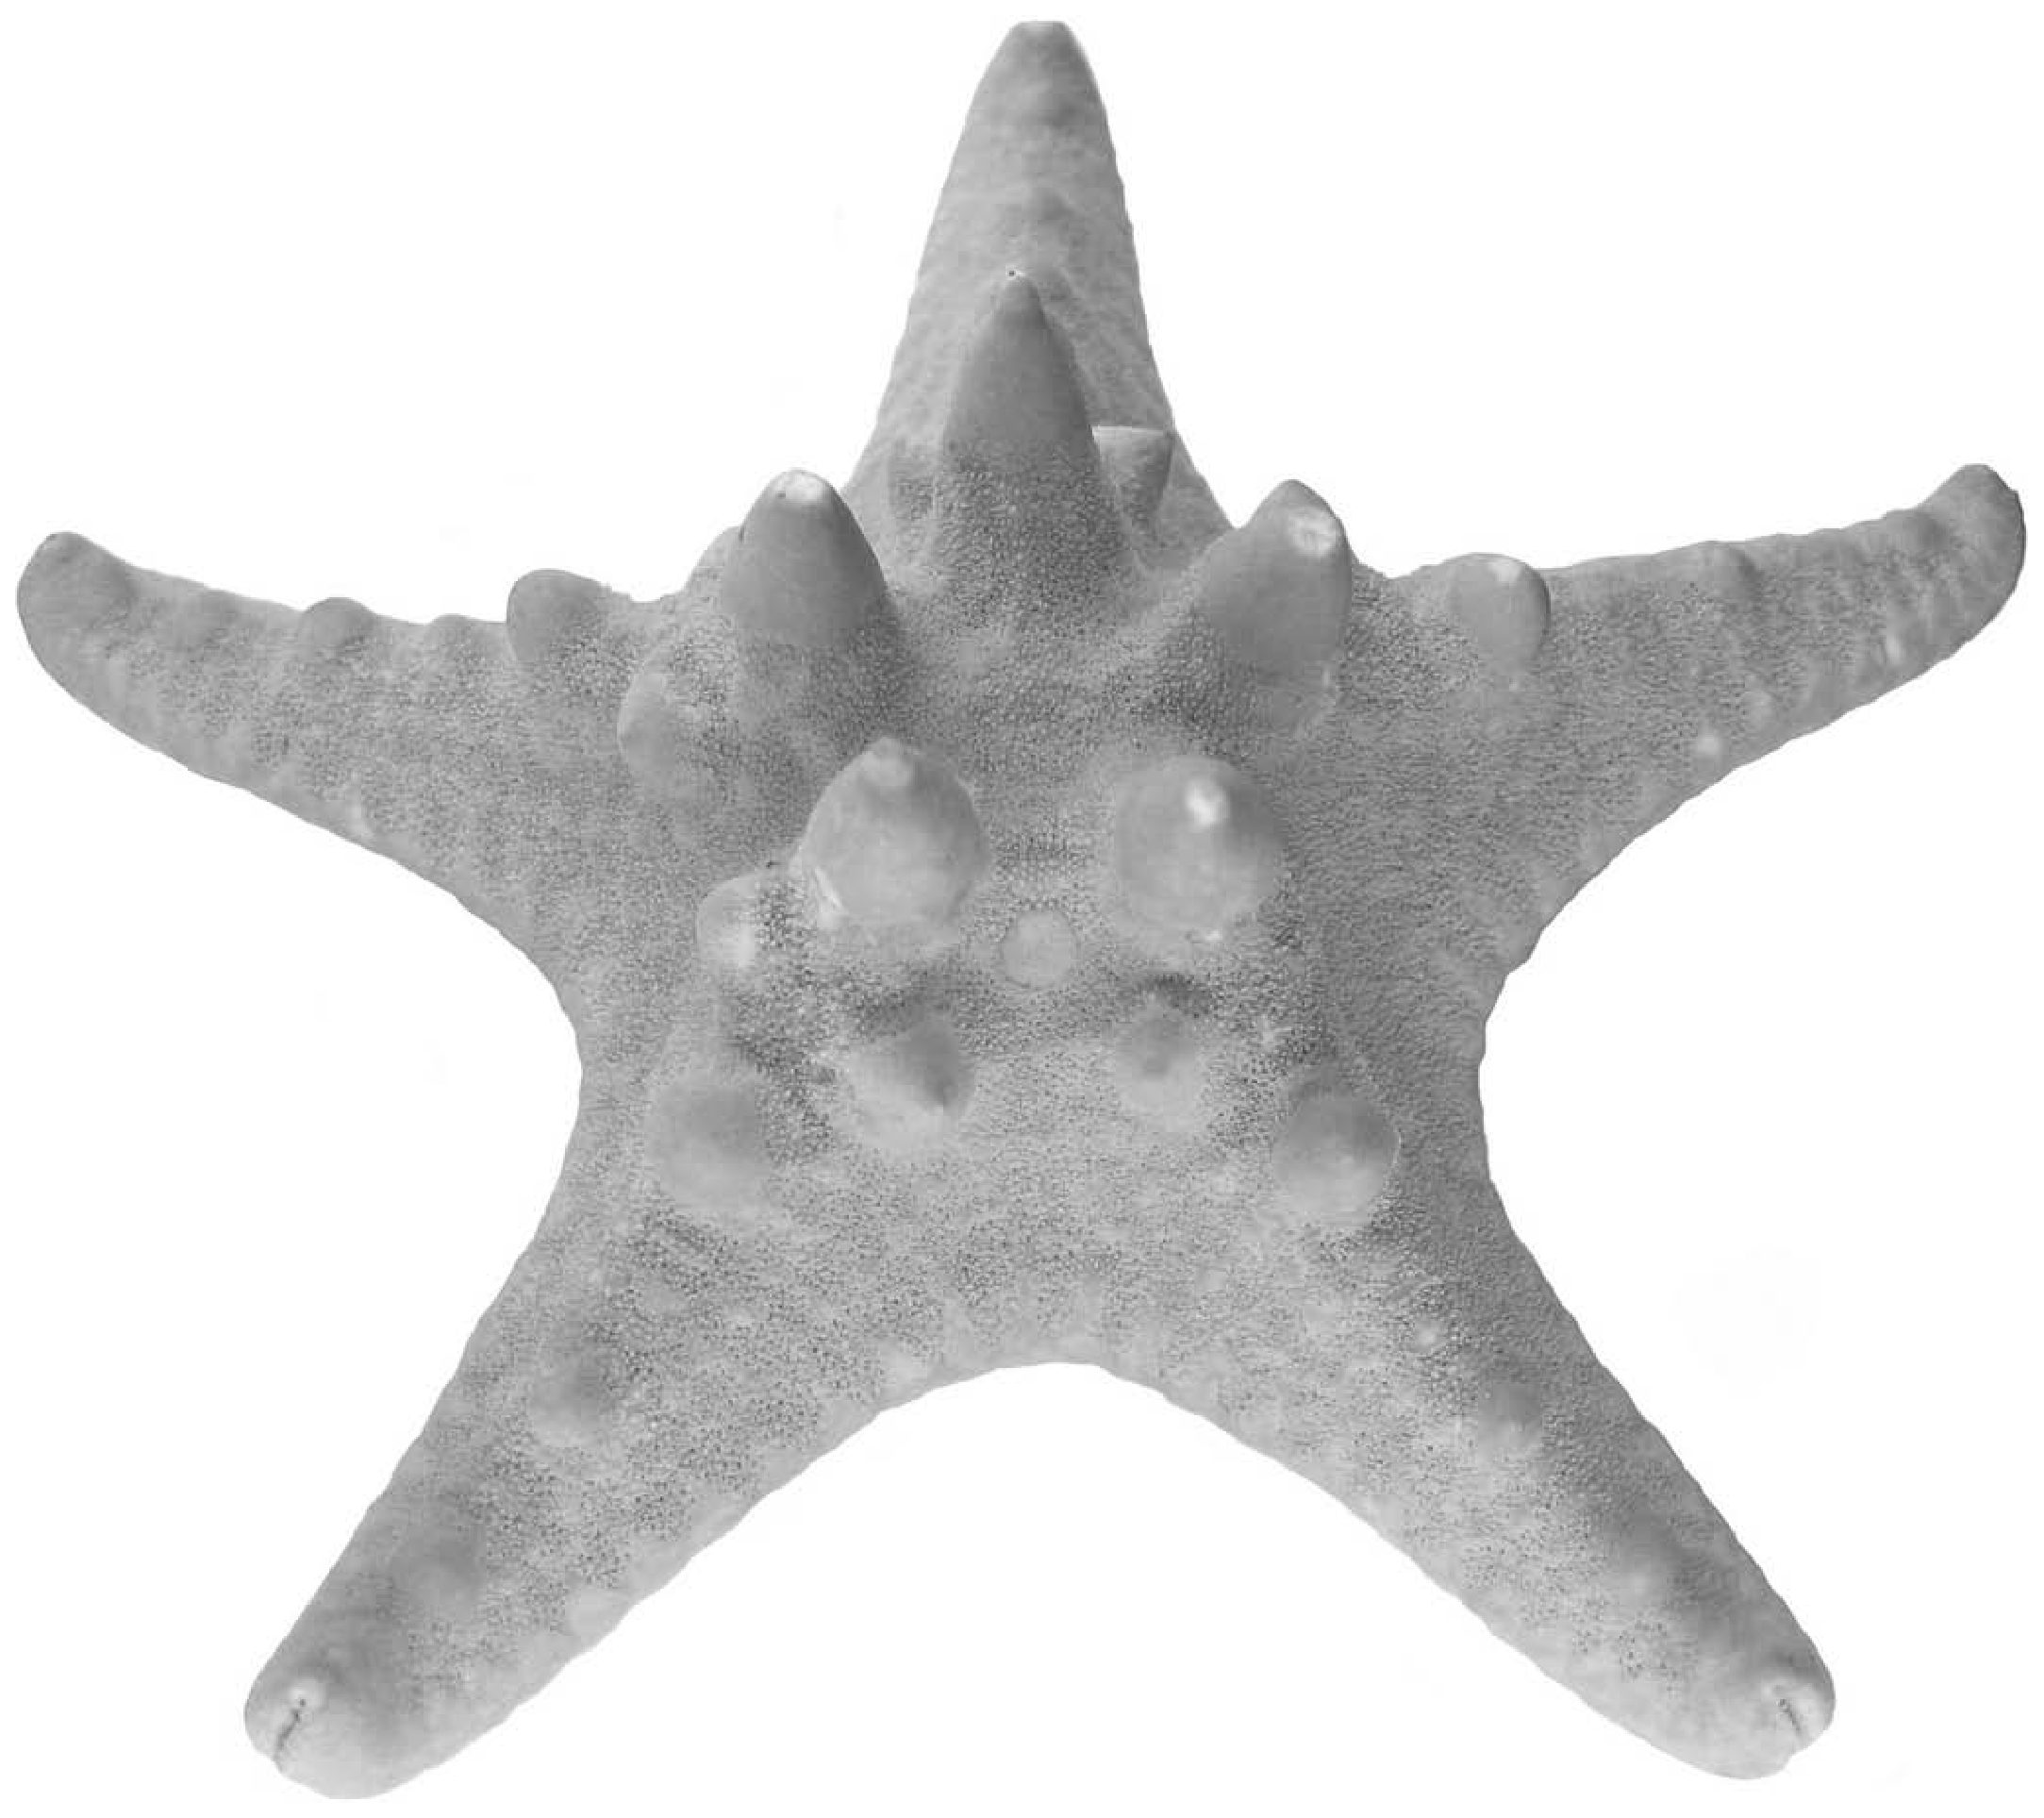
\includegraphics[width=0.45\textwidth]{pic/starfish}}
    ~~~
    \subcaptionbox{Рисунок, зашифрованный AES-128\label{fig:starfish-aes-128-ecb}}{ 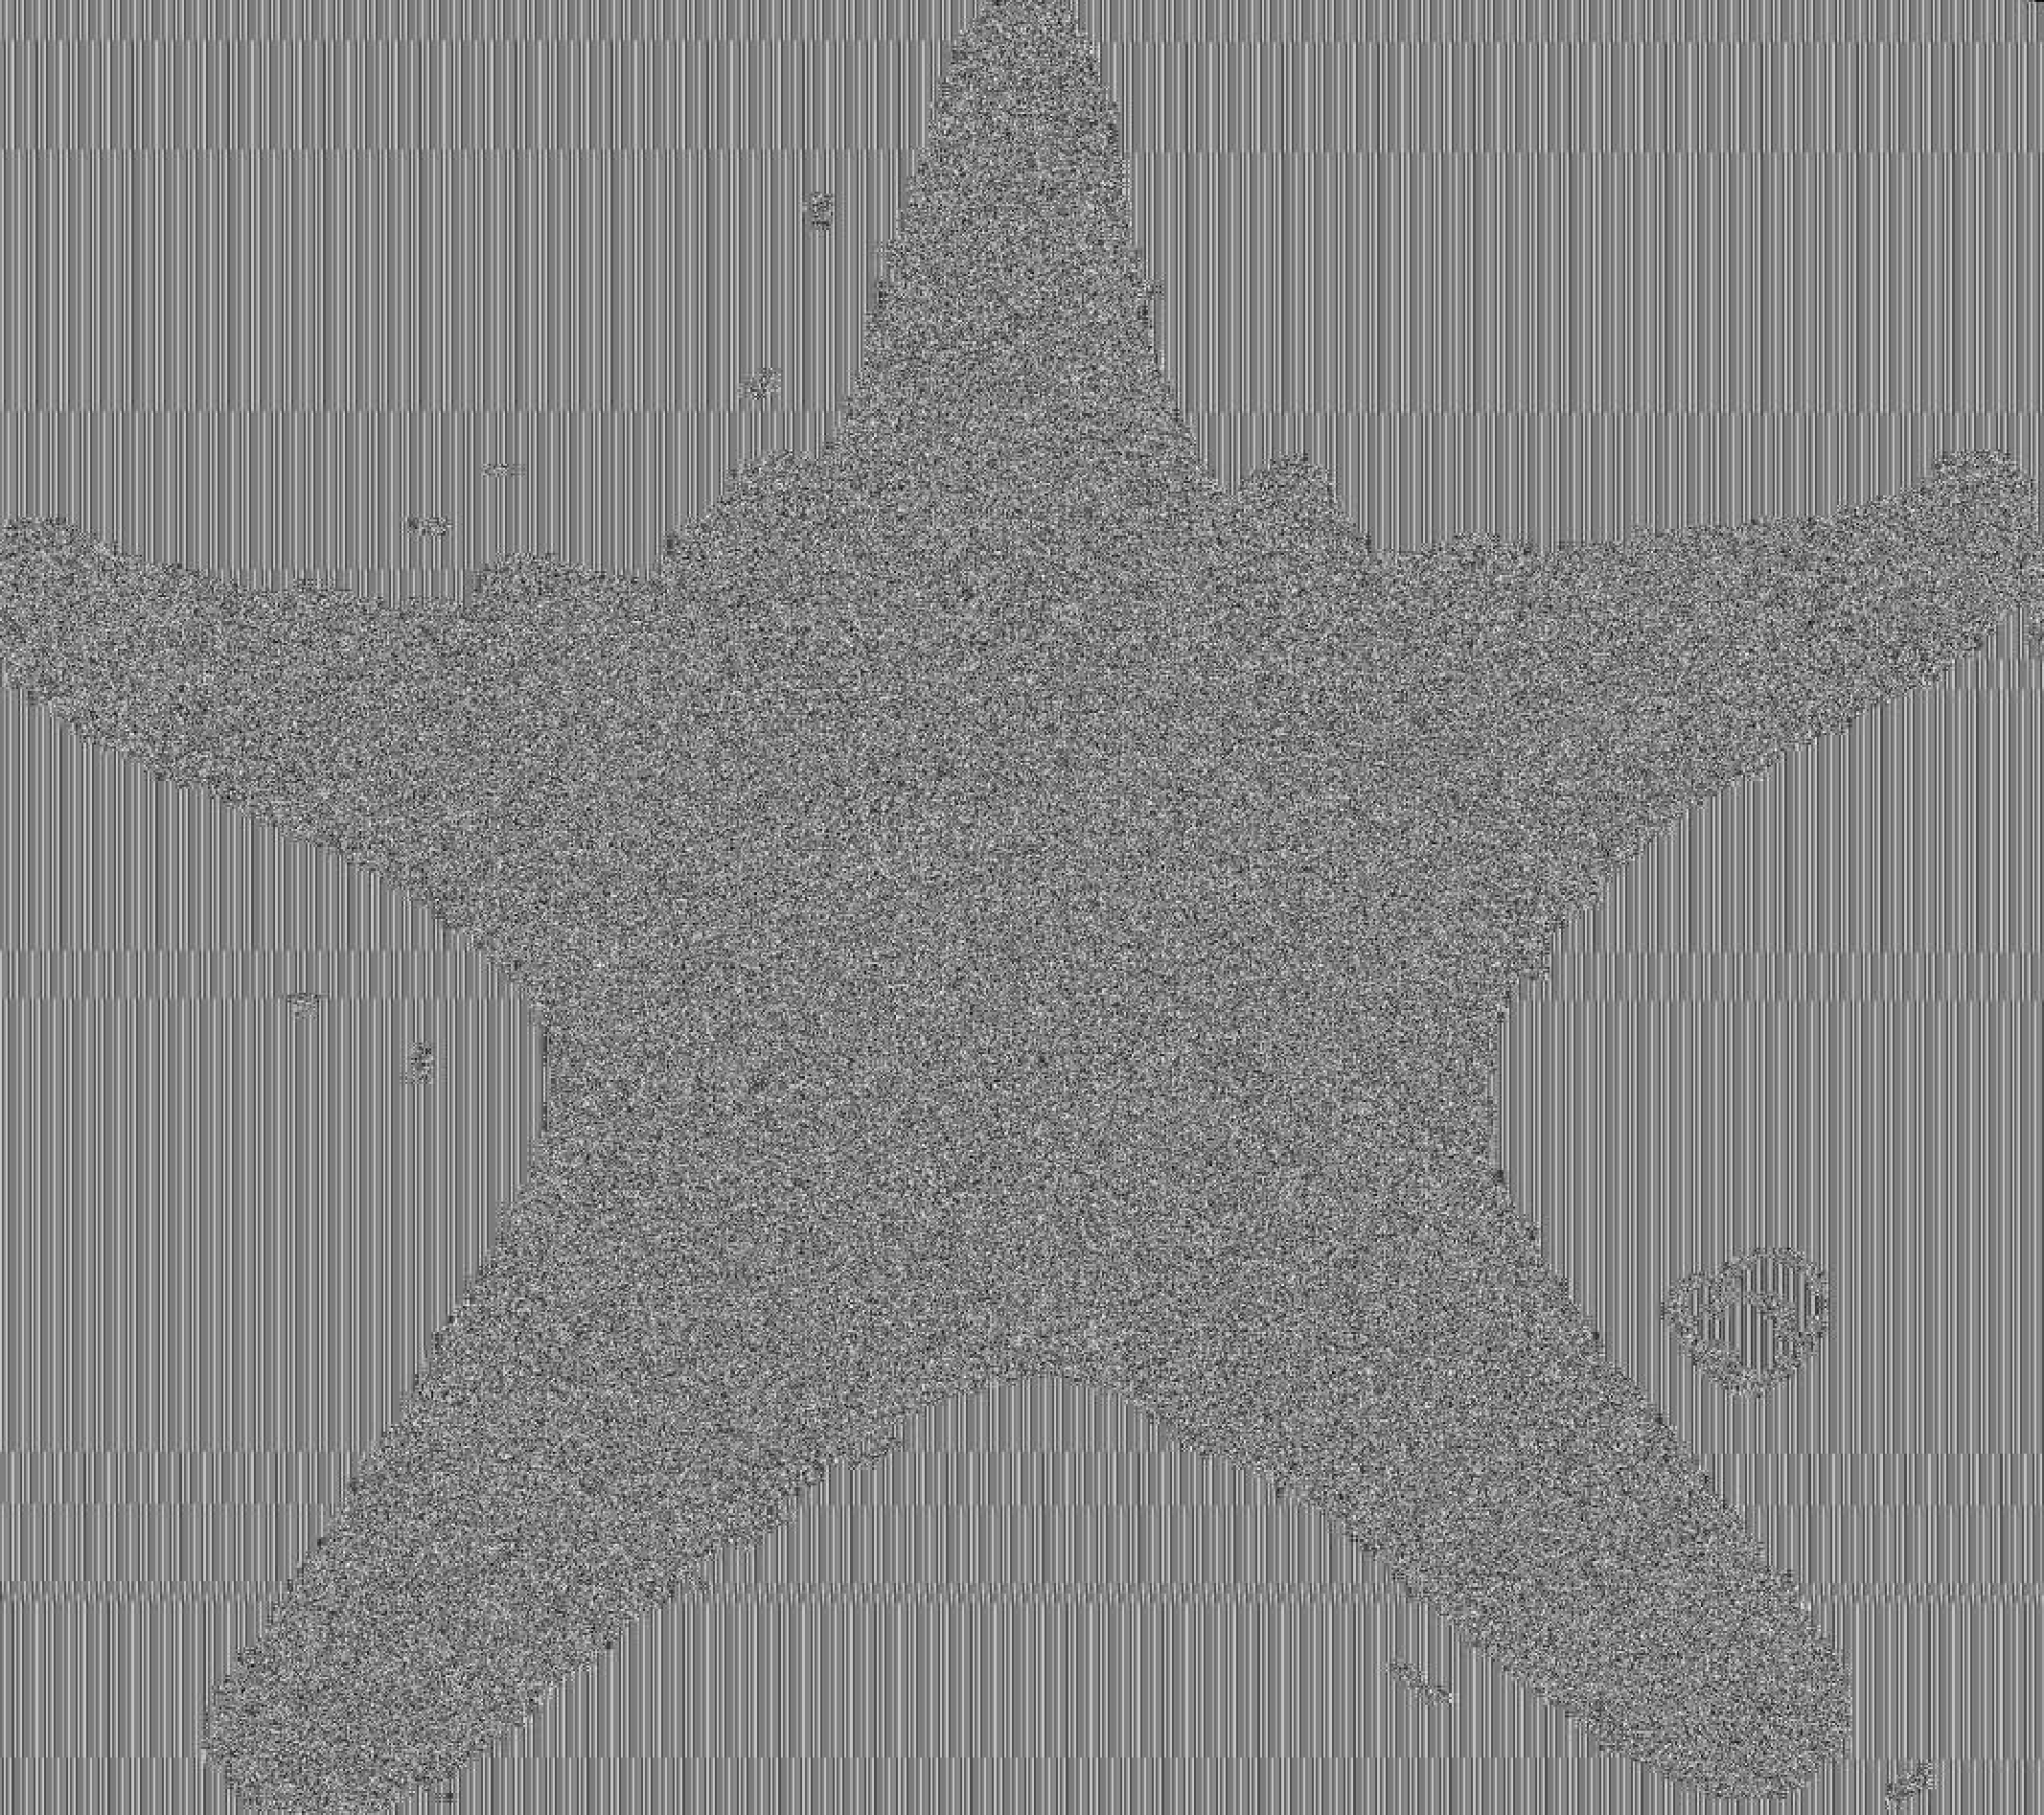
\includegraphics[width=0.45\textwidth]{pic/starfish-aes-128-ecb}}
    \caption{Шифрование в режиме электронной кодовой книги\label{fig:ecb-demo}}
\end{figure}
BMP файл в данном случае содержит в самом начале стандартный заголовок (ширина, высота, количество цветов), и далее идёт массив 24-битовых значений цвета пикселей, взятых построчно сверху вниз. В массиве много последовательностей нулевых байтов, так как пиксели белого фона кодируются 3 нулевыми байтами. В AES размер блока равен 16 байтам, и, значит, каждые $\frac{16}{3}$ подряд идущих пикселей белого фона шифруются одинаково, позволяя различить изображение в зашифрованном файле.

%На рис.~\ref{fig:ecb-demo} приведён пример шифрования графического файла логотипа Википедии в формате BMP, 24 бита цветности на пиксель (рис.~\ref{fig:wikilogo}), блочным шифром AES с длиной ключа 128 бит в режиме электронной кодовой книги (рис.~\ref{fig:wikilogo-aes-128-ecb}). В начале зашифрованного файла был восстановлен стандартный заголовок BMP формата. Как видно, на зашифрованном рисунке возможно даже прочитать надпись.
%\begin{figure}[!ht]
%    \centering
%    \subfloat[Исходный рисунок]{\label{fig:wikilogo}\includegraphics[width=0.45\textwidth]{pic/wikilogo}}
%    ~~~
%    \subfloat[Рисунок, зашифрованный AES-128]{\label{fig:wikilogo-aes-128-ecb}\includegraphics[width=0.45\textwidth]{pic/wikilogo-aes-128-ecb}}
%    \caption{Шифрование в режиме электронной кодовой книги.}
%    \label{fig:ecb-demo}
%\end{figure}

%Возможно воссоздание структуры информации -- например, пингвин на рис.~\ref{fig:tux-ecbmode}. Картинка с пингвином записана в формате BMP и зашифрована DES в режиме электронной кодовой книги.
%\begin{figure}[!ht]
%    \centering
%    \includegraphics[width=0.3\textwidth]{pic/tux-ecb}
%    \caption{Картинка с пингвином, зашифрованная в режиме электронной кодовой книги.}
%    \label{fig:tux-ecbmode}
%\end{figure}


\subsection{Сцепление блоков шифртекста}

В режиме сцепления блоков шифртекста (\langen{Cipher Block Chaining, CBC}) перед шифрованием текущего блока открытого текста предварительно производится его суммирование по модулю $2$ с предыдущим блоком зашифрованного текста, что и осуществляет <<сцепление>> блоков. Процедура шифрования имеет вид:
\[ \begin{array}{l}
    C_j = E_K(M_j \oplus C_{j-1}), ~ j = 1, 2, \dots, n,
\end{array} \]
где $C_0 = \textrm{IV}$ (сокр. от \langen{Initialization Vector}) -- блок, называемый вектором инициализации. Другое название -- синхропосылка.

Благодаря сцеплению, \emph{одинаковым} блокам открытого текста соответствуют \emph{различные} шифрованные блоки. Это затрудняет криптоаналитику статистический анализ потока шифрованных блоков.

На приёмной стороне расшифрование осуществляется по правилу:
\[ \begin{array}{l}
    D_K(C_j) = M_j \oplus C_{j-1}, ~ j=1, 2, \dots, n,\\
    M_{j} = D_K(C_j) \oplus C_{j-1}.
\end{array} \]

Блок $C_0 = \textrm{IV}$ должен быть известен легальному получателю шифрованных сообщений. Обычно криптограф выбирает его случайно и вставляет на первое место в поток шифрованных блоков. Сначала передают блок $C_0$, а затем шифрованные блоки $C_1, C_2, \ldots, C_n$.

В разных пакетах блоки $C_0$ должны выбираться независимо. Если их выбрать одинаковыми, то возникают проблемы, аналогичные проблемам в режиме ECB. Например, часто первые нешифрованные блоки $M_1$ в разных пакетах бывают одинаковыми. Тогда одинаковыми будут и первые шифрованные блоки.

Однако случайный выбор векторов инициализации также имеет свои недостатки. Для выбора такого вектора необходим хороший генератор случайных чисел. Кроме того, каждый пакет удлиняется на один блок.

Для каждого сеанса передачи пакета нужны такие процедуры выбора $C_0$, которые известны криптографу и легальному пользователю. Одним из решений является использование так называемых \emph{одноразовых меток}. Каждому сеансу присваивается уникальное число. Его уникальность состоит в том, что оно используется только один раз и никогда не должно повторяться в других пакетах. В англоязычной научной литературе оно обозначается как \emph{Nonce}, то есть сокращение от <<Number used once>>\index{одноразовая метка}.

Обычно одноразовая метка состоит из номера сеанса и дополнительных данных, обеспечивающих уникальность. Например, при двустороннем обмене шифрованными сообщениями одноразовая метка может состоять из номера сеанса и индикатора направления передачи. Размер одноразовой метки должен быть равен размеру шифруемого блока. После определения одноразовой метки $\textrm{Nonce}$ вектор инициализации вычисляется в виде:
    \[ C_0 = \textrm{IV} = E_K(\textrm{Nonce}). \]

Этот вектор используется в данном сеансе для шифрования открытого текста в режиме CBC. Заметим, что блок $C_0$ передавать в сеансе необязательно, если приёмная сторона знает заранее дополнительные данные для одноразовой метки. Вместо этого достаточно вначале передать только номер сеанса в открытом виде. Принимающая сторона добавляет к нему дополнительные данные и вычисляет блок $C_0$, необходимый для расшифрования в режиме CBC. Это позволяет сократить издержки, связанные с удлинением пакета. Например, для шифра AES длина блока $C_0$ равна $16$ байтов. Если число сеансов ограничить величиной $2^{32}$ (вполне приемлемой для большинства приложений), то для передачи номера пакета понадобится только $4$ байта.


\subsection{Обратная связь по выходу}

В предыдущих режимах входными блоками для устройств шифрования были непосредственно блоки открытого текста.
В режиме обратной связи по выходу (OFB от Output FeedBack) блоки открытого текста непосредственно на вход устройства шифрования не поступают. Вместо этого устройство шифрования генерирует псевдослучайный поток байтов, который суммируется по модулю $2$ с открытым текстом для получения шифрованного текста. Шифрование осуществляют по правилу:
\[ \begin{array}{l}
    K_0 = \textrm{IV}, \\
    K_j = E_K(K_{j-1}), ~ j = 1, 2, \dots, n, \\
    C_j = K_j \oplus M_j.
\end{array} \]

Здесь текущий ключ $K_j$ есть результат шифрования предыдущего ключа $K_{j-1}$. Начальное значение $K_0$ известно криптографу и легальному пользователю. На приёмной стороне расшифрование выполняют по правилу:
\[ \begin{array}{l}
    K_0 = \textrm{IV}, \\
    K_j = E_K(K_{j-1}), ~ j = 1, 2, \dots, n, \\
    M_j = K_j \oplus C_j.
\end{array} \]

Как и в режиме CBC, вектор инициализации $\textrm{IV}$ может быть выбран случайно и передан вместе с шифрованным текстом, либо вычислен на основе одноразовых меток. Здесь особенно важна уникальность вектора инициализации.

Достоинство этого режима состоит в полном совпадении операций шифрования и расшифрования. Кроме того, в этом режиме не надо проводить операцию дополнения открытого текста.


\subsection{Обратная связь по шифрованному тексту}

В режиме обратной связи по шифрованному тексту (CFB от Cipher FeedBack) ключ $K_j$ получается с помощью процедуры шифрования предыдущего шифрованного блока $C_{j-1}$. Может быть использован не весь блок $C_{j-1}$, а только его часть. Как и в предыдущем случае, начальное значение ключа $K_0$ известно криптографу и легальному пользователю:
\[ \begin{array}{l}
    K_0 = \textrm{IV}, \\
    K_j = E_K(C_{j-1}), ~ j = 1, 2, \dots, n,\\
    C_j = K_j \oplus M_j.
\end{array} \]

У этого режима нет особых преимуществ по сравнению с другими режимами.


\subsection{Счётчик}

В режиме счётчика (CTR от Counter) правило шифрования имеет вид, похожий на режим обратной связи по выходу (OFB), но позволяющий вести независимое (параллельное) шифрование и расшифрование блоков:
\[ \begin{array}{l}
    K_j = E_K(\textrm{Nonce} ~\|~ j - 1), ~ j = 1, 2, \dots, n, \\
    C_j = M_j \oplus K_j,
\end{array} \]
где $\textrm{Nonce} ~\|~ j - 1$ -- конкатенация битовой строки одноразовой метки $\textrm{Nonce}$ и номера блока, уменьшенного на единицу.
%Для стандарта AES значение $\textrm{Nonce}$ занимает 16 бит, номер блока -- 48 бит. С одним ключом выполняется шифрование $2^{48}$ блоков.

Правило расшифрования идентичное:
\[ \begin{array}{l}
    M_j = C_j \oplus K_j. \\
\end{array} \]


\section{Некоторые свойства блочных шифров}

\subsection{Обратимость схемы Фейстеля}
\selectlanguage{russian}

Покажем, что обратимость схемы Фейстеля не зависит от выбора функции $F$.

Напомним, что схема Фейстеля -- это итеративное шифрование, в котором выход подаётся на вход следующей итерации по правилу:
\[ \begin{array}{l}
    L_i = R_{i-1}, \\
    R_i = L_{i-1} \oplus F(R_{i-1}, K_i), \\
\end{array} \]
\[
    (L_0,R_0) \rightarrow (L_1,R_1) \rightarrow \ldots \rightarrow (L_n,R_n).
\]

При расшифровании используется та же схема, только левая и правая части меняются местами перед началом итераций, а ключи раунда подаются в обратном порядке:
    \[ R_i = L_{i-1} \oplus F(R_{i-1}, K_{n+1-i}), \]
\[ \begin{array}{l}
    L_0^* = R_n = L_{n-1} \oplus F(R_{n-1}, K_n), \\
    R_0^* = L_n = R_{n-1}, \\
    \\
%\end{array} \]
%\[ \begin{array}{l}
    L_1^* = R_{n-1}, \\
    R_1^* = L_{n-1} \oplus F(R_{n-1}, K_n) \oplus F(R_{n-1}, K_n) = L_{n-1}, \\
    \dots.
\end{array} \]


\subsection{Схема Фейстеля без s-блоков}
\selectlanguage{russian}

Пусть функция $F$ является простой линейной комбинацией некоторых битов правой части и ключа раунда относительно операции XOR. Тогда можно записать систему линейных уравнений битов выхода $y_i$ относительно битов входа $x_i$ и ключа $k_i$ после всех 16 раундов в виде
    \[ y_i = \left(\sum_{i=0}^{n_1} a_i x_i\right) \oplus \left(\sum_{i=0}^{n_2} b_i k_i\right), \]
где суммирование производится по модулю 2, коэффициенты $a_i$ и $b_i$ известны и равны 0 или 1, количество битов в блоке открытого текста равно $n_1$, количество битов ключа равно $n_2$.

Имея открытый текст и шифртекст, легко найти ключ. Без знания открытых текстов, выполняя XOR шифртекстов, можно найти XOR открытых текстов, что может привести к возникновению благоприятных для взлома шифра условий. Во-первых, это может позволить провести атаку на различение сообщений. Во-вторых, в широко распространенных случаях, когда известны форматы сообщений, отдельные поля или распределение символов открытого текста, появляется возможность осуществить атаку перебором с учётом множества уравнений, полученных XOR шифртекстов.

Для предотвращения подобных атак используются s-блоки замены для создания нелинейности в уравнениях выхода $y_i$ относительно сообщения и ключа.


\subsubsection[Схема Фейстеля в ГОСТ 28147-89 без s-блоков]{Схема Фейстеля в~ГОСТ~28147-89 без~s-блоков}

В отличие от устаревшего алгоритма DES блочный шифр ГОСТ без s-блоков намного сложнее для взлома, так как для него нельзя записать систему линейных уравнений:
\[
    \begin{array}{l}
        L_1 = R_0, \\
        R_1 = L_0 \oplus ((R_0 \boxplus K_1) \lll 11), \\
    \end{array}
\] \[
    \begin{array}{l}
        L_2 = R_1 = L_0 \oplus ((R_0 \boxplus K_1) \lll 11), \\
        R_2 = L_1 \oplus (R_1 \boxplus K_2)  = \\
        ~~~~~= R_0 \oplus (((L_0 \oplus ((R_0 \boxplus K_1) \lll 11)) \boxplus K_2) \lll 11). \\
    \end{array}
\]

Операция $\boxplus$ нелинейна по XOR. Например, только на трёх операциях $\oplus$, $\boxplus$ и $\lll f(R_i)$ без использования s-блоков построен блочный шифр RC5, который по состоянию на 2010 г. не был взломан.


\subsection{Лавинный эффект}
\selectlanguage{russian}

\subsubsection{Лавинный эффект в DES}

Оценим число раундов, за которое в DES достигается полный лавинный эффект\index{лавинный эффект}, предполагая \emph{случайное} расположение бит перед расширением, s-блоками ($s$ -- substitute, блоки замены) и XOR.

Пусть на входе правой части $R_i$ содержится $r$ бит, на которые уже распространилось влияние одного бита, выбранного вначале. После расширения получим
    \[ n_1 \approx \min(1.5 \cdot r, 32) \]
зависимых бит. Предполагая случайные попадания в 8 s-блоков, мы увидим, что, согласно задаче о размещении, биты попадут в
    \[ s_2 = 8 \left( 1 - \left( 1 - \frac{1}{{8}{n_1}} \right)^{n_1} \right) \approx 8 \left( 1 - e^{-\frac{n_1}{8}} \right) \]
s-блоков. Одно из требований NSA к s-блокам заключалось в том, чтобы изменение каждого бита входа \emph{изменяло} 2 бита выхода. Мы предположим, что каждый бит входа s-блока \emph{влияет} на все 4 бита выхода. Зависимыми станут
    \[ n_2 = 4 \cdot s_2 \approx 32 \left( 1 - e^{-\frac{n_1}{8}} \right) \]
бит. При дальнейшем XOR с величиной $L_i$, содержащей $l$ зависимых бит, результатом будет
    \[ n_3 \approx n_2 + l  - \frac{n_2 l}{32} \]
зависимых бит.

\begin{table}[!ht]
    \centering
    \caption{Распространение влияния 1 бита левой части в DES\label{tab-DES-avalance-effect}}
    \begin{tabular}{||c||c||c|c|c||}
        \hline
        \multirow{3}{*}{Раунд} & $L_i$ & \multicolumn{3}{|c||}{$R_i$} \\
        \cline{2-5}
        & & Расширение & s-блоки & $R_{i+1} = f(R_i) \oplus L_i$ \\
        & $l$ & $r \rightarrow n_1$ & $n_1 \rightarrow n_2$ & $(n_2, l) \rightarrow n_3$ \\
        \hline \hline
        0 & 1 & 0 & 0 & 0 \\
        1 & 0 & 0 & 0 & $(0,1) \rightarrow 1$ \\
        2 & 1 & $1 \rightarrow 1.5$ & $1.5 \rightarrow 5.5$ & $(5.5, 0) \rightarrow 5.5$ \\
        3 & 5.5 & $5.5 \rightarrow 8.2$ & $8.2 \rightarrow 20.5$ & $(20.5, 1) \rightarrow 20.9$ \\
        4 & 20.9 & $20.9 \rightarrow 31.3$ & $31.3 \rightarrow 32$ & $(32, 20.9) \rightarrow 32$ \\
        5 & 32 & 32 & 32 & 32 \\
      \hline
    \end{tabular}
\end{table}

В таблице~\ref{tab-DES-avalance-effect} приводится расчёт распространения одного бита левой части. Посчитано число зависимых битов по раундам в предположении об их случайном расположении и о том, что каждый бит на входе s-блока \emph{влияет} на все биты выхода. Полная диффузия достигается за 5 раундов, что совпадает с экспериментальной проверкой. Для достижения максимального лавинного эффекта требуется аккуратно выбрать расширение, s-блоки, а также перестановку в функции $F$.


\subsubsection{Лавинный эффект в ГОСТ 28147-89}

Лавинный эффект\index{лавинный эффект} по входу обеспечивается $(4 \times 4)$ s-блоками и циклическим сдвигом влево на $11 \neq 0 \mod 4$.

\begin{table}[!ht]
    \centering
    \caption{Распространение влияния 1 бита левой части в ГОСТ 28147-89\label{tab:GOST-avalance-effect}}
    \resizebox{\textwidth}{!}{ \begin{tabular}{||c||c|c|c|c|c|c|c|c||c|c|c|c|c|c|c|c||}
        \hline
        \multirow{2}{*}{Раунд} & \multicolumn{8}{|c||}{$L_i$} & \multicolumn{8}{|c||}{$R_i$} \\
        \cline{2-17}
              & 1 & 2 & 3 & 4 & 5 & 6 & 7 & 8   &   1 & 2 & 3 & 4 & 5 & 6 & 7 & 8 \\
        \hline \hline
        0     &   &   &   &   &   &   &   & 1   &     &   &   &   &   &   &   &   \\
        1     &   &   &   &   &   &   &   &     &     &   &   &   &   &   &   & 1 \\
        2     &   &   &   &   &   &   &   & 1   &     &   &   &   & 3 & 1 &   &   \\
        3     &   &   &   &   & 3 & 1 &   &     &     & 3 & 4 & 1 &   &   &   & 1 \\
        4     &   & 3 & 4 & 1 &   &   &   & 1   &   4 & 1 &   &   & 3 & 1 & 3 & 4 \\
        5     & 4 & 1 &   &   & 3 & 1 & 3 & 4   &     & 3 & 4 & 4 & 4 & 4 & 4 & 1 \\
        6     &   & 3 & 4 & 4 & 4 & 4 & 4 & 1   &   4 & 4 & 4 & 4 & 4 & 3 & 3 & 4 \\
        7     & 4 & 4 & 4 & 4 & 4 & 3 & 3 & 4   &   4 & 4 & 4 & 4 & 4 & 4 & 4 & 4 \\
        8     & 4 & 4 & 4 & 4 & 4 & 4 & 4 & 4   &   4 & 4 & 4 & 4 & 4 & 4 & 4 & 4 \\
      \hline
    \end{tabular} }
\end{table}

Из таблицы~\ref{tab:GOST-avalance-effect} видно, что на каждом раунде число зависимых битов увеличивается в среднем на 4 в результате сдвига и попадания выхода s-блока предыдущего раунда в два s-блока следующего раунда. Показано распространение зависимых битов в группах по 4 бита в левой и правой частях без учёта сложения с ключом раунда. Предполагается, что каждый бит на входе s-блока влияет на все биты выхода. Число раундов для достижения полного лавинного эффекта без учёта сложения с ключом -- 8. Экспериментальная проверка для s-блоков, используемых Центробанком РФ, показывает, что требуется 8 раундов.


\subsubsection{Лавинный эффект в AES}

В первом раунде один бит оказывает влияние на один байт в операции <<замена байтов>> и затем на столбец из четырёх байтов в операции <<перемешивание столбцов>>\index{лавинный эффект}.

Во втором раунде операция <<сдвиг строк>> сдвигает байты изменённого столбца на разное число байтов по строкам, в результате получаем диагональное расположение изменённых байтов, то есть в каждой строке присутствует по изменённому байту. Далее, в результате операции <<перемешивания столбцов>> изменение распространяется от байта в столбце на весь столбец и, следовательно, на всю матрицу.

Диффузия по входу достигается за 2 раунда.


\subsection{Двойное и тройное шифрования}\index{шифрование!двойное}\index{шифрование!тройное}
\selectlanguage{russian}

В конце XX-го века, когда ненадёжность существующего стандарта DES\index{шифр!DES} уже была очевидна, а нового стандарта ещё не было, стали распространены техники двойного и тройного шифрования, когда к одному блоку текста последовательно применяется несколько преобразований на разных ключах.

Например, двойное шифрование\index{шифрование!двойное} 2DES\index{шифр!2DES} использует два разных ключа $K_1$ и $K_2$ для шифрования одного блока текста дважды:
\[ E_{K1, K2} \left( M \right) \equiv E_{K1} \left( E_{K2} \left( M \right) \right). \]

Так как функция шифрования\index{функция!шифрования} DES не образует группу\index{группа} (\cite{Kaliski:Rivest:Sherman:1988, Campbell:Wiener:1993}), то данное преобразование не эквивалентно однократному шифрованию на каком-нибудь третьем ключе. То есть для произвольных $K_1$ и $K_2$ нельзя подобрать такой $K_3$, что
\[E_{K1} \left( E_{K2} \left( M \right) \right) \equiv E_{K3} \left( M \right).\]

Тем самым размер ключевого пространства (количество различных ключей шифрования, если считать за ключ пару $K_1$ и $K_2$) увеличивается с $2^{56}$ до $2^{112}$ (без учёта проверочных бит). Однако из-за атаки <<встреча посередине>>\index{атака!встреча посередине} (\langen{meet in the middle}) фактическая криптостойкость увеличилась не более чем до $2^{57}$.

Тройной DES (\langen{triple DES, 3DES})\index{шифрование!тройное}\index{шифр!3DES} использует тройное преобразование. Причём в качестве второй функции используется функция \emph{расшифрования}:
\[ E_{K1, K2, K3} \left( M \right) \equiv E_{K1} \left( D_{K2} \left( E_{K3} \left( M \right) \right) \right). \]

\begin{itemize}
	\item Вариант $K_1 \neq K_2 \neq K_3$ является наиболее защищённым, ключевое пространство увеличивается до $2^{168}$.
	\item Вариант $K_1 \neq K_2$, $K_1 = K_3$ увеличивает ключевое пространство до $2^{112}$, но защищён от атаки <<встреча посередине>>\index{атака!встреча посередине}, в отличие от 2DES\index{шифр!2DES}.
	\item Вариант $K_1 = K_2 = K_3$ эквивалентен однократному преобразованию DES\index{шифр!DES}. Его можно использовать для обеспечения совместимости.
\end{itemize}

Оценим сложность атак на 2DES\index{шифр!2DES} и 3DES\index{шифр!3DES}.

\subsubsection{Атака на двойное шифрование}

%Для упрощения записи введём обозначение последовательного шифрования $E_{K_1}( E_{K_2}( \dots E_{K_n}(M) \dots)) \equiv E{K_1} \circ E_{K_2} (M)$ и назовём его суперпозицией функций $E_{K_i}$.

Атака основана на предположении, что у криптоаналитика есть возможность получить либо шифртекст для любого открытого текста\index{атака!с известным шифртекстом} (\langen{Chosen Plaintext Attack, CPA}), либо открытый текст по шифртексту\index{атака!с известным открытым текстом} (\langen{Chosen Ciphertext Attack, CCA}), но неизвестен ключ шифрования, который и нужно найти.

Шифрование в 2DES\index{шифр!2DES}:
    \[ C = E_{K_1}( E_{K_2}(M)). \]
Запишем $D_{K_1}(C) = E_{K_2}(M)$. Пусть время одного шифрования -- $T_E$, время одного сравнения блоков $T_{=} \approx 2^{-10} T_E$.

Атака для нахождения ключей без использования памяти занимает время
    \[ T = 2^{56 + 56} (T_E + T_{=}) \approx 2^{112} T_E. \]

Можно заранее вычислить значения $E_{K_2}(M)$ для всех ключей и построить таблицу: индекс -- $E_{K_2}(M)$, значения поля -- набор ключей $K_2$, которые соответствуют этому значению. Атака для нахождения ключей требует времени
    \[ T = 2 \cdot 2^{56} T_E + 2^{56} T_{=} \approx 2^{57} T_E \]
и памяти $M = 56 \cdot 2^{56} \approx 2^{62}$ бит ($\approx 504$ Пбайт), учитывая прямой доступ по значению к возможным ключам. При нахождении соответствия берётся другая пара (открытый текст, шифртекст) и проверяется равенство для определения, являются ли ключи правильными или нет.

По отношению к CCA и CPA криптостойкость 2DES\index{шифр!2DES} эквивалентна обычному DES\index{шифр!DES} с использованием 26 ГиБ памяти.

\subsubsection{Атака на тройное шифрование}

Атака для нахождения ключей (CCA\index{атака!с известным шифртекстом}, CPA\index{атака!с известным открытым текстом}) на наиболее стойкий вариант 3DES\index{шифр!3DES} (все три ключа $K_1$, $K_2$ и $K_3$ выбираются независимо) требует времени $T \approx 2^{168} T_E$ без использования дополнительной памяти.

Для построения таблицы запишем
    \[ D_{K_2}( D_{K_1}( C)) = E_{K_3} (M). \]
Таблица строится аналогично 2DES\index{шифр!2DES} для $E_{K_3}(M)$. С использованием памяти атака занимает время $T = 2^{112} T_E$ и память $M = 26$ GiB.


\index{шифр!блочный|)}

\chapter{Генераторы псевдослучайных чисел}\label{chapter-generators}
\selectlanguage{russian}

Для работы многих криптографических примитивов необходимо уметь получать случайные числа:
\begin{itemize}
	\item вектор инициализации для отдельных режимов сцепления блоков должен быть случайным числом (см. раздел~\ref{section-block-chaining});
	\item для генерации пар открытых и закрытых ключей необходимы случайные числа (см. главу~\ref{chapter-public-key});
	\item стойкость многих криптографических протоколов ключей (см. главу~\ref{chapter-protocols}) основывается в том числе на выработке случайных чисел (\langen{nonce}), которые не может предугадать злоумышленник.
\end{itemize}

Генератором случайных чисел (\langen{random number generator})\index{генератор!случайных чисел} мы будем называть процесс\footnote{Есть и строгое математическое определение генератора в общем смысле. Генератором называется функция $g: \left\{0, 1\right\}^{n} \to \left\{0, 1\right\}^{q\left(n\right)}$, вычислимая за полиномиальное время. Однако мы пока не будем использовать это определение, чтобы показать разницу между истинно случайными числами и псевдослучайными.}, результатом работы которого является случайная последовательность чисел, а именно такая, что зная произвольное число предыдущих чисел последовательности (и способ их получения), даже теоретически нельзя предсказать следующее с вероятностью больше заданной. К таким случайным процессам можно отнести:

\begin{itemize}
	\item результат работы счётчика элементарных частиц, работа с которым включена в лабораторный практикум по общей физике для студентов первого курса МФТИ;
	\item время между нажатиями клавиш на клавиатуре персонального компьютера или расстояние, которое проходит <<мышь>> во время движения;
	\item время между двумя пакетами, полученными сетевой картой;
	\item тепловой шум, измеряемый звуковой картой на входе аналогового микрофона, даже при отсутствии самого микрофона.
\end{itemize}

Хотя для всех этих процессов можно предсказать приблизительное значение (чётное или нечётное), его последний бит будет оставаться достаточно случайным для практических целей. С учётом данной поправки их можно называть надёжными или качественными генераторами случайных чисел.

Однако к генератору случайных чисел предъявляются и другие требования. Кроме уже указанного критерия \emph{качественности} или \emph{надёжности}, генератор должен быть \emph{быстрым} и \emph{дешёвым}. Быстрым -- чтобы получить большой объём случайной информации за заданный период времени. И дешёвым -- чтобы его можно было бы использовать на практике. Количество случайной информации от перечисленных выше генераторов составляет не более десятков килобайт в секунду (для теплового шума) и значительно меньше, если мы будем требовать ещё и равномерность распределения полученных случайных чисел.

С целью получения большего объёма случайной информации используют специальные алгоритмы, которые называют генераторами псевдослучайных чисел (ГПСЧ). ГПСЧ -- это детерминированный алгоритм, выходом которого является последовательность чисел, обладающая свойством случайности. Работу ГПСЧ можно описать следующей моделью. На подготовительном этапе оперативная память, используемая алгоритмом, заполняется начальным значением (\langen{seed}). Далее на каждой итерации своей работы ГПСЧ выдаёт на выход число, которое является функцией от состояния оперативной памяти алгоритма, и меняет содержимое своей памяти по определённым правилам. Содержимое оперативной памяти называется \emph{внутренним состоянием} генератора.

Как и у любого алгоритма, у ГПСЧ есть определённый размер используемой оперативной памяти\footnote{Только алгоритмы с фиксированным размером используемой оперативной памяти и можно называть \emph{генераторами} в строгом математическом смысле этого слова, как следует из определения.}. Исходя из практических требований, предполагается, что размер оперативной памяти для ГПСЧ сильно ограничен. Так как память алгоритма ограничена, то ограничено и число различных внутренних состояний алгоритма. В силу того, что выдаваемые ГПСЧ числа являются функцией от внутреннего состояния, то любой ГПСЧ, работающий с ограниченным размером оперативной памяти и не принимающий извне дополнительной информации, будет иметь \emph{период}. Для генератора с памятью в $n$ бит максимальный период, очевидно, равен $2^n$.

Качество детерминированного алгоритма, то есть то, насколько полученная последовательность обладает свойством случайной, можно оценить с помощью тестов, таких как набор тестов NIST (\langen{National Institute of Standards and Technology}, США,~\cite{NIST:2001}). Данный набор содержит большое число различных проверок, включая частотные тесты бит и блоков, тесты максимальных последовательностей в блоке, тесты матриц и так далее.

\input{linear-congruential-generator}

\input{lfsr}

\input{crypto-random}

\input{bbs_generator}

\section{КСГПСЧ на основе РСЛОС}

Как уже упоминалось ранее, использование РСЛОС в качестве ГПСЧ не является криптографически стойким. Однако можно использовать комбинацию из нескольких регистров сдвига, чтобы в результате получить быстрый, простой (дешёвый) и надёжный (криптографически стойкий) генератор псевдослучайных чисел.

\input{generators_with_multiple_shift_registers}

\input{generators_with_nonlinear_transformations}

\input{majority_generators}


\input{stream-ciphers}

\input{hash-functions}

\input{public-key}

\subimport*{protocols/}{index}

\chapter{Разделение секрета}\index{схема!разделения секрета|(}
\selectlanguage{russian}

\section{Пороговые схемы}

Идея \emph{пороговой} $(K, N)$-схемы\index{разделение секрета!пороговое} разделения общего секрета среди $N$ пользователей состоит в следующем. Доверенная сторона хочет распределить некий секрет $K_0$ между $N$ пользователями таким образом, что:
\begin{itemize}
    \item любые $m_1: K \leq m_1 \leq N$, легальных пользователей могут получить секрет (или доступ к секрету), если предъявят свои секретные ключи;
    \item любые $m_2: m_2 < K$, легальных пользователей не могут получить секрет и не могут определить (вычислить) этот секрет, даже решив трудную в вычислительном смысле задачу.
\end{itemize}

Далее рассмотрены три случая: $(K, N)$-схема Блэкли, $(K, N)$-схема Шамира и простая $(N,N)$-схема.

\input{secret-sharing-blackleys}

\input{secret-sharing-shamirs}

\input{secret-sharing-xor}

\section{Распределение секрета по коалициям}

\subsection{Схема для нескольких коалиций}

Предположим, что имеется $N$ легальных пользователей
    \[ \{ U_1, U_2, \dots, U_N \}, \]
которым нужно сообщить (открыть, предоставить в доступ) общий секрет $K$.

Секрет может быть доступен только определённым коалициям\index{распределение секрета!по коалициям}, например:
\[ \begin{array}{l}
    C_1 = \{ U_1, U_2 \}, \\
    C_2 = \{ U_1, U_3, U_4 \}, \\
    C_3 = \{ U_2, U_3 \}, \\
    \dots
\end{array} \]
При этом ни одна из коалиций $C_i, ~ i = 1, 2, \dots$ не должна быть подмножеством другой коалиции.


\example
Имеется 4 участника:
    \[ \{ U_1, U_2, U_3, U_4 \}, \]
которые образуют 3 коалиции:
\[ \begin{array}{l}
    C_1 = \{ U_1, U_2 \}, \\
    C_2 = \{ U_1, U_3 \}, \\
    C_3 = \{ U_2, U_3, U_4 \}. \\
\end{array} \]
Распределение частичных секретов между ними представлено в виде таблицы~\ref{tab:secret-share-coalition-1}, в которой введены следующие обозначения: $a_1, b_1, c_2, c_3$ -- случайные числа из кольца $\Z_M$. В строках таблицы содержатся частичные секреты каждого из пользователей, в столбцах таблицы показаны частичные секреты, соответствующие каждой из коалиций.

\begin{table}[!ht]
    \centering
    \caption{Распределение секрета по определённым коалициям\label{tab:secret-share-coalition-1}}
    \begin{tabular}{|c||c|c|c|}
        \hline
              & $C_1 = \{ U_1, U_2 \}$ & $C_2 = \{U_1, U_3 \}$ & $C_3 = \{ U_2, U_3, U_4 \}$ \\
        \hline \hline
        $U_1$ & $a_1$     & $b_1$     & -- \\
        $U_2$ & $K - a_1$ & --        & $c_2$ \\
        $U_3$ & --        & $K - b_1$ & $c_3$  \\
        $U_4$ & --        & --        & $K - c_2 - c_3$ \\
        \hline
    \end{tabular}
\end{table}

Как видно из приведённых данных, суммирование по модулю $M$ чисел, записанных в каждом из столбцов таблицы, открывает секрет $K$.
\exampleend


\example

%\section{Схема разделения секрета на монотонных булевых функциях}
%\example
В системе распределения секрета доверенный
%с использованием монотонных булевых функций
центр использует кольцо $\Z_m$ целых чисел по модулю $m$. Требуется разделить секрет $K$ между $5$ пользователями:
    \[ \{ U_1, U_2, U_3, U_4, U_5 \} \]
так, чтобы восстановить секрет могли только коалиции:
\[ \begin{array}{lll}
    C_1 = \{ U_1, U_2 \},      & & C_2 = \{ U_1, U_3 \}, \\
    C_3 = \{ U_2, U_3, U_4 \}, & & C_4 = \{ U_2, U_3, U_5 \}, \\
    C_5 = \{ U_3, U_4, U_5 \}, & & C_6 = \{ U_1, U_2, U_3 \}. \\
\end{array} \]

Заданное множество коалиций с доступом не является минимальным, так как одни коалиции входят в другие:
    \[ C_1 \subset C_6, ~ C_2 \subset C_6. \]
Исключая $C_6$, получим минимальное множество коалиций с доступом к секрету: ни одна из оставшихся коалиций не входит в другую $C_i \nsubseteq C_j$ для $i \neq j$. Пользователям выдаются тени по минимальному множеству коалиций с доступом. В строках таблицы~\ref{tab:secret-share-coalition-2} содержатся частичные секреты каждого из пользователей, в столбцах таблицы показаны частичные секреты, соответствующие каждой из коалиций.

\begin{table}[!ht]
    \centering
    \caption{Распределение секрета по определённым коалициям\label{tab:secret-share-coalition-2}}
    \begin{tabular}{|c||c|c|c|c|c|}
        \hline
              & $C_1$     & $C_2$     & $C_3$           & $C_4$           & $C_5$  \\
        \hline \hline
        $U_1$ & $a_1$     & $b_1$     & --              & --              & -- \\
        $U_2$ & $K - a_1$ & --        & $c_2$           & $d_2$           & --\\
        $U_3$ & --        & $K - b_1$ & $c_3$           & $d_3$           & $e_3$ \\
        $U_4$ & --        & --        & $K - c_2 - c_3$ & --              & $e_4$ \\
        $U_5$ & --        & --        & --              & $K - d_2 - d_3$ & $K - e_3 - e_4$ \\
        \hline
    \end{tabular}
\end{table}

Тени выбираются случайно из кольца $\mathbb{\Z}_m$. В результате у пользователей будут тени. 
\exampleend

\subsection{Схема Брикелла для нескольких коалиций}\index{схема разделения секрета!Бриккела|(}\index{схема!Бриккела|(}
\selectlanguage{russian}

Рассмотрим схему Брикелла (\langen{Ernest Francis Brickell},~\cite{Brickell:1990}) разделения секрета по коалициям.

По-прежнему
    \[ \{ U_1, U_2, \dots, U_N \} \]
-- легальные пользователи. Пусть $\Z_p$ -- кольцо целых чисел по модулю $p$. Рассмотрим векторы
    \[ \mathcal{U} = \left\{ (u_1, u_2, \dots, u_d) \right\}, ~~ u_i \in \Z_p \]
длины $d$. Каждому пользователю $U_i, ~ i = 1, \dots, N$ ставится в соответствие вектор
    \[ \varphi(U_i) \in \mathcal{U}, ~~ i = 1, \dots, N. \]

Тогда каждой из коалиций, например
    \[ C_1 = \{ U_1, U_2, U_3 \}, \]
соответствует набор векторов
    \[ \varphi(U_1), \varphi(U_2), \varphi(U_3). \]
Эти векторы должны быть выбраны так, чтобы их линейная оболочка \emph{содержала} вектор
    \[ (1, 0, 0, \dots, 0) \]
длины $d$. Линейная оболочка любого набора векторов, не образующих коалицию, \emph{не должна} содержать вектор $(1, 0, 0, \dots, 0)$ длины $d$.

Пусть $K_0 \in \Z_p$ -- общий секрет. Распределение секрета производится следующим образом. Сначала вычисляется вектор $(K_0, K_1, \dots, K_{d-1})$, где первая координата -- это общий секрет, а остальные координаты выбираются из $\Z_p$ случайно. Затем вычисляются скалярные произведения:
\[\begin{array}{l}
	\left( \left( K_0, K_1, \dots, K_{d-1} \right), ~ \varphi(U_1) \right) ~=~ a_1, \\
	\left( \left( K_0, K_1, \dots, K_{d-1} \right), ~ \varphi(U_2) \right) ~=~ a_2, \\
	\dots \\
	\left( \left( K_0, K_1, \dots, K_{d-1} \right), ~ \varphi(U_N) \right) ~=~ a_N. \\
\end{array}\]

Пользователям $U_i, ~ i = 1, 2, \dots, N$ выдаются их частичные секреты:
    \[ U_i \colon \left\{ \varphi(U_i), a_i \right\}. \]

Пусть коалиция $C$ -- допустимая, например:
    \[ C = C_1 = \{ U_1, U_2, U_3 \}. \]

Тогда члены коалиции совместно находят такие коэффициенты $\lambda_1, \lambda_2, \lambda_3$, что
    \[ \lambda_1\varphi(U_1)+\lambda_2\varphi(U_2)+\lambda_3\varphi(U_3) ~=~ (1,0, \dots, 0). \]

После этого вычисляется выражение
\[\begin{array}{l}
    \lambda_1 a_1 + \lambda_2 a_2 + \lambda_3 a_3 = \\
    = \left( \left( K_0, K_1, \dots, K_{d-1} \right), ~ \lambda_1 \varphi(U_1) + \lambda_2 \varphi(U_2) + \lambda_3 \varphi(U_3) \right) = \\
    = \left( \left( K_0, K_1, \dots, K_{d-1} \right), ~ \left( 1, 0, \dots, 0 \right) \right) =  K_0, \\
\end{array}\]
которое и является общим секретом.

%\section{Схема разделения секрета в векторном пространстве Бриккела}
%
%В схеме Бриккела для $n$ пользователей $\{ U_1, U_2, \ldots, U_n \}$ Центр выбирает $k$-мерные векторы $\varphi(U_i)$ над полем $\mathbb{\Z}_p$ так, чтобы их линейная нетривиальная комбинация над полем $\mathbb{\Z}_p$ могла равняться единичному вектору
%    \[ (1,0,0, \ldots, 0) = \sum\limits_{i=1}^{n} c_i \ \varphi(U_i), ~ c_i \in  \mathbb{\Z}_p. \]
%Центр пользователю $i$ присваивает \emph{открытый, публично доступный} вектор $\varphi(U_i)$.
%
%Для разделения секрета $K$ Центр выбирает случайные числа $a_2, a_3, \ldots, a_n$, составляет вектор $\bar{a} = (K, a_2, a_3, \ldots, a_n)$ и выдаёт каждому пользователю \emph{секретную} тень $s_i = \bar{a} \cdot \varphi(U_i)$.
%
%Восстановление секрета производится
%    \[ K = \bar{a} \cdot (1,0,\ldots,0) = \bar{a} \cdot \sum\limits_{i=1}^{n} c_i \varphi(U_i) = \sum\limits_{i=1}^{n} c_i s_i, \]
%так как из открытых векторов $\varphi(U_i)$ пользователи могут найти $c_i$.
%
%Восстановить секрет могут только те коалиции пользователей, для которых нетривиальная комбинация векторов $\varphi(U_i)$ даёт единичный вектор.

\example
Для сети из $n = 4$ участников
    \[ \{ U_1, U_2, U_3, U_4 \} \]
выбраны следующие векторы длины $k = 3$ над полем $\Z_{23}$:
\[ \begin{array}{l}
    \varphi(U_1) = (0,2,0), \\
    \varphi(U_2) = (2,0,7), \\
    \varphi(U_3) = (0,5,7), \\
    \varphi(U_4) = (0,2,9). \\
\end{array} \]
Найдём все коалиции, которые могут раскрыть секрет.

Запишем
    \[ (1,0,0) = c_1 (0,2,0) + c_2 (2,0,7) + c_3 (0,5,7) + c_4 (0,2,9). \]
Ясно, что $c_2 \neq 0$ и коалициями пользователей, которые дают единичный вектор и, следовательно, могут восстановить секрет, являются:
\[ \begin{array}{l}
    C_1 = \{ U_1, U_2, U_3 \}, \\
    C_2 = \{ U_1, U_2, U_4 \}, \\
    C_3 = \{ U_2, U_3, U_4 \}. \\
\end{array} \]

Пусть доверенный центр для секрета $K = 4$ выбрал вектор $\bar{a} = (4, 2, 9)$. Тогда участники получают тени:
    \[ s_1 = (4,2,9) \cdot (0,2,0) = 4 \mod 23, \]
    \[ s_2 = (4,2,9) \cdot (2,0,7) = 2 \mod 23, \]
    \[ s_3 = (4,2,9) \cdot (0,5,7) = 4 \mod 23, \]
    \[ s_4 = (4,2,9) \cdot (0,2,9) = 16 \mod 23. \]

Возьмём коалицию $C_1 = \{ U_1, U_2, U_3 \}$ и вычислим коэффициенты $c_i$:
    \[ (1,0,0) = c_1 (0,2,0) + c_2 (2,0,7) + c_3 (0,5,7), \]
\[ \begin{array}{l}
    c_1 = 7 \mod 23, \\
    c_2 = 12 \mod 23, \\
    c_3 = 11 \mod 23. \\
\end{array} \]

Найдём секрет:
    \[ K = 7 \cdot 4 + 12 \cdot 2 + 11 \cdot 4 = 4 \mod 23.\]
\exampleend

\index{схема разделения секрета!Бриккела|)}\index{схема!Бриккела|)}


\index{схема!разделения секрета|)}

\chapter{Примеры систем защиты}

\subsection{Протокол <<Kerberos>>}\index{протокол!Kerberos|(}\label{section-protocols-kerberos}
\selectlanguage{russian}

В данном разделе будет описан протокол аутентификации сторон с единственным доверенным центром. Сетевой протокол <<Kerberos>> использует эти идеи при объединении нескольких доверенных центров в единую сеть для обеспечения надёжности и отказоустойчивости. Подробнее о сетевом протоколе <<Kerberos>> смотрите в разделе~\ref{section-kerberos}.

Как и в протоколе Нидхема~---~Шрёдера, инициирующий абонент (Алиса) общается только с выделенным доверенным центром, получая от него два пакета с зашифрованным сессионным ключом -- один для себя, а второй -- для вызываемого абонента (Боба). Однако в отличие от Нидхема~---~Шрёдера\index{протокол!Нидхема~---~Шрёдера} в рассматриваемом протоколе зашифрованные пакеты содержат также метку времени $T_T$ и срок действия сессионного ключа $L$ (от \langen{lifetime} -- срок жизни). Что позволяет, во-первых, защититься от рассмотренной в предыдущем разделе атаки повтором. А, во-вторых, позволяет доверенному центру в некотором смысле управлять абонентами, заставляя их получать новые сессионные ключи по истечению заранее заданного времени $L$.

\begin{figure}
    \centering
    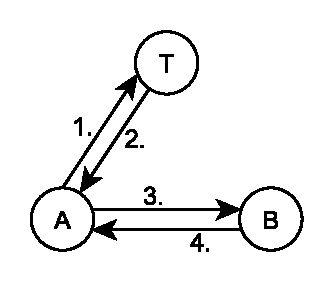
\includegraphics[width=0.5\textwidth]{pic/key_distribution-kerberos}
    \caption{Схема взаимодействия абонентов и доверенного центра в протоколе <<Kerberos>>\label{fig:key_distribution-kerberos}}
\end{figure}

\begin{protocol}
	\item[(1)] $ Alice \to \{ A, B \} \to Trent $
	\item[(2)] $ Trent \to \{ E_A \left( T_T, L, K, B \right), E_B \left( T_T, L, K, A \right) \} \to Alice $
	\item[(3)] $ Alice \to \{ E_B \left( T_T, L, K, A \right), E_K \left( A, T_A \right) \} \to Bob $
	\item[(4)] $ Bob \to \{ E_K \left( T_T + 1 \right) \} \to Alice $
\end{protocol}

Обратите внимание, что на третьем проходе за счёт использования метки времени от доверенного центра $T_T$ вместо случайной метки от Боба $R_B$ позволяет сократить количество проходов на один по сравнению с протоколом Нидхема~---~Шрёдера\index{протокол!Нидхема~---~Шрёдера}. Также наличие метки времени делает ненужным и предварительную генерацию случайной метки Алисой и её передачу на первом шаге.

Метка времени $T_A$ в сообщении $E_K \left( A, T_A \right)$ позволяет Бобу убедиться, что Алиса владеет текущим сессионным ключом $K$. Если расшифрованная метка $T_A$ сильно отличается от текущего времени, значит либо этот пакет из другого сеанса протокола, либо не от Алисы вообще.

Интересно отметить, что пакеты $E_A \left( T_T, L, K, B \right)$ и $E_B \left( T_T, L, K, A \right)$ одинаковы по своему формату. В некотором смысле их можно назвать сертификатами сессионного ключа для Алисы и Боба. Причём все подобные пары пакетов можно сгенерировать заранее (например, в начале дня), выложить на общедоступный ресурс, предоставить в свободное использование и выключить доверенный центр (он своё дело уже сделал -- сгенерировав эти пакеты). И до момента времени $T_T + L$ этими <<сертификатами>> можно пользоваться. Но только если вы являетесь одной из допустимых пар абонентов. Конечно, эта идея непрактична -- ведь количество таких пар растёт как квадрат от числа абонентов. Однако интересен тот факт, что подобные пакеты можно сгенерировать заранее. Эта идея нам пригодится при рассмотрении инфраструктуры открытых ключей (\langen{public key infrastructure, PKI}).

\index{протокол!Kerberos|)}

\section{Pretty Good Privacy}
\selectlanguage{russian}

В качестве примера передачи файлов по сети с обеспечением аутентификации, конфиденциальности и целостности рассмотрим систему PGP (\langen{Pretty Good Privacy}), разработанную Филом Циммерманном (\langen{Phil Zimmermann}) в 1991 г. Изначально система предлагалась к использованию для защищённой передачи электронной почты. Стандартом PGP является OpenPGP. Примерами реализации стандарта OpenPGP являются GNU Privacy Guard (GPG) и netpgp, разработанные в рамках проектов GNU и NetBSD соответственно.

Каждый пользователь обладает одной или несколькими парами из закрытого и открытого ключей. Ключи используются как для расшифрования получаемых пользователем сообщений, так и для генерации электронных подписей отправляемых сообщений. Также пользователь хранит открытые ключи других участников системы, чтобы иметь возможность отправлять им зашифрованные сообщения и аутентифицировать отправителей принимаемых сообщений.

В системе PGP каждое передаваемое сообщение подписывается закрытым ключом отправителя, затем сообщение шифруется блочной криптосистемой на случайно выбранном секретном сеансовом ключе. Сам сеансовый ключ шифруется криптосистемой с открытым ключом на открытом ключе получателя.

Свои закрытые ключи отправитель хранит в зашифрованном виде. Набор ключей называется связкой закрытых ключей. Шифрование закрытых ключей в связке производится симметричным шифром\index{шифр!симметричный}, ключом которого является функция от пароля, вводимого пользователем. Шифрование закрытых ключей, хранимых на компьютере, является стандартной практикой для защиты от утечки, например, в случае взлома ОС, утери ПК и~т.\,д.

Набор открытых ключей других пользователей называется связкой открытых ключей.

\begin{figure}[!ht]
	\centering
	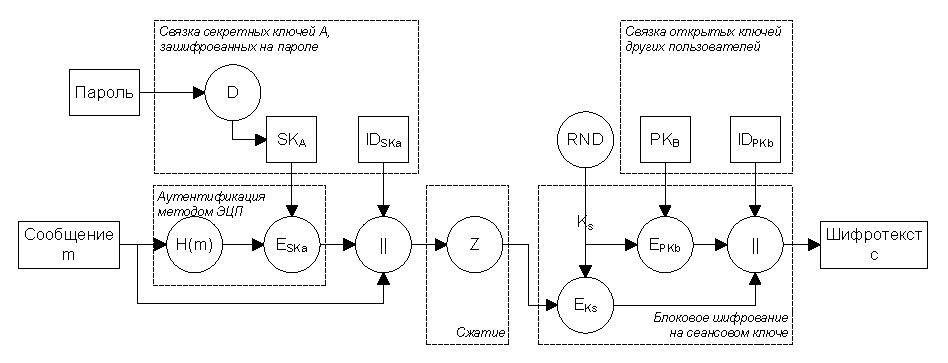
\includegraphics[width=0.9\textwidth]{pic/pgp}
	\caption{Схема обработки сообщения в PGP\label{fig:pgp}}
\end{figure}

На рис.~\ref{fig:pgp} представлена схема обработки сообщения в PGP для передачи от $A$ к $B$. Использование аутентификации, сжатия и блочного шифрования является опциональным. Обозначения на рисунке следующие:
\begin{itemize}
    \item Пароль -- пароль, вводимый отправителем для расшифрования связки своих закрытых ключей;
    \item $D$ -- расшифрование блочной криптосистемы для извлечения секретного ключа ЭП отправителя;
    \item $SK_A$ -- закрытый ключ ЭП отправителя;
    \item $ID_{SKa}$ -- идентификатор ключа ЭП отправителя, по которому получатель определяет, какой ключ из связки открытых ключей использовать для проверки подписи;
    \item $m$ -- сообщение (файл) для передачи;
    \item $h(m)$ -- криптографическая хэш-функция;
    \item $E_{SKa}$ -- схема ЭП на секретном ключе $SK_A$;
    \item $\|$ -- конкатенация битовых строк;
    \item $Z$ -- сжатие сообщения алгоритмом компрессии;
    \item $RND$ -- криптографический генератор псевдослучайной последовательности;
    \item $K_s$ -- сгенерированный псевдослучайный сеансовый ключ;
    \item $E_{Ks}$ -- блочное шифрование на секретном сеансовом ключе $K_s$;
    \item $PK_B$ -- открытый ключ получателя;
    \item $ID_{PKb}$ -- идентификатор открытого ключа получателя, по которому получатель определяет, какой ключ из связки закрытых ключей использовать для расшифрования сеансового ключа;
    \item $E_{PKb}$ -- шифрование сеансового ключа криптосистемой с открытым ключом на открытом ключе $B$;
    \item $c$ -- зашифрованное подписанное сообщение.
\end{itemize}


\section{Протокол SSL/TLS}\index{протокол!SSL/TLS}
\selectlanguage{russian}

Протокол SSL (\langen{Secure Sockets Layer}) был разработан компанией Netscape. Начиная с версии 3, протокол развивается как открытый стандарт TLS (\langen{Transport Layer Security}). Протокол SSL/TLS обеспечивает защищённое соединение по незащищённому каналу связи на прикладном уровне модели TCP/IP. Протокол встраивается между прикладным и транспортным уровнями стека протоколов TCP/IP. Для обозначения <<новых>> протоколов, полученных с помощью инкапсуляции прикладного уровня (HTTP\index{протокол!HTTP}, FTP\index{протокол!FTP}, SMTP\index{протокол!SMTP}, POP3\index{протокол!POP3}, IMAP\index{протокол!IMAP} и~т.\,д.) в SSL/TLS, к обозначению добавляют суффикс <<S>> (<<Secure>>): HTTPS\index{протокол!HTTPS}, FTPS\index{протокол!FTPS}, POP3S\index{протокол!POP3S}, IMAPS\index{протокол!IMAPS} и~т.\,д.

Протокол обеспечивает следующее:
\begin{itemize}
    \item Одностороннюю или взаимную аутентификацию клиента и сервера по открытым ключам сертификата X.509. В Интернете, как правило, делается \emph{односторонняя} аутентификация веб-сервера браузеру клиента, то есть только веб-сервер предъявляет сертификат (открытый ключ и ЭП к нему от вышележащего УЦ).
    \item Создание сеансовых симметричных ключей для шифрования и кода аутентификации сообщения для передачи данных в обе стороны.
    \item Конфиденциальность\index{конфиденциальность} -- блочное или потоковое шифрование передаваемых данных в обе стороны.
    \item Целостность\index{целостность} -- аутентификацию отправляемых сообщений в обе стороны имитовставкой\index{имитовставка} $\HMAC(K,M)$, описанной ранее.
\end{itemize}

Рассмотрим протокол TLS последней версии 1.2.


\subsection{Протокол <<рукопожатия>>}

Протокол <<рукопожатия>> (\langen{Handshake Protocol}) производит аутентификацию и создание сеансовых ключей между клиентом $C$ и сервером $S$.

\begin{enumerate}
    \item $C \rightarrow S$:
        \begin{enumerate}
            \item ClientHello: ~ 1) URI сервера, ~ 2) одноразовая метка $N_C$\index{одноразовая метка}, ~ 3) поддерживаемые алгоритмы шифрования, кода аутентификации сообщений, хэширования, ЭП и сжатия.
        \end{enumerate}

    \item $C \leftarrow S$:
        \begin{enumerate}
            \item ServerHello: одноразовая метка $N_S$, поддерживаемые сервером алгоритмы.

            После обмена набором желательных алгоритмов сервер и клиент по единому правилу выбирают общий набор алгоритмов.
            \item Server Certificate: сертификат X.509v3 сервера с запрошенным URI (URI нужен в случае нескольких виртуальных веб-серверов с разными URI на одном узле c одним IP-адресом).
            \item Server Key Exchange Message: информация для создания предварительного общего секрета $premaster$ длиной 48 байтов в виде: ~ 1) обмена по протоколу Диффи~---~Хеллмана\index{протокол!Диффи~---~Хеллмана} с клиентом (сервер отсылает $(g, g^a)$), ~ 2)Обмена по другому алгоритму с открытым ключом, ~ 3) разрешения клиенту выбрать ключ.
            \item Электронная подпись к Server Key Exchange Message на ключе сертификата сервера для аутентификации сервера клиенту.
            \item Certificate Request: опциональный запрос сервером сертификата клиента.
            \item Server Hello Done: идентификатор конца транзакции.
        \end{enumerate}

    \item $C \rightarrow S$:
        \begin{enumerate}
            \item Client Certificate: сертификат X.509v3 клиента, если он был запрошен сервером.
            \item Client Key Exchange Message: информация для создания предварительного общего секрета $premaster$ длиной 48 байтов в виде: ~ 1) либо обмена по протоколу Диффи~---~Хеллмана\index{протокол!Диффи~---~Хеллмана} с сервером (клиент отсылает $g^b$, в результате обе стороны вычисляют ключ $premaster = g^{ab}$), ~ 2) либо обмена по другому алгоритму, ~ 3) либо ключа, выбранного клиентом и зашифрованного на открытом ключе из сертификата сервера.
            \item Электронная подпись к Client Key Exchange Message на ключе сертификата клиента для аутентификации клиента серверу (если клиент использует сертификат).
            \item Certificate Verify: результат проверки сертификата сервера.
            \item Change Cipher Spec: уведомление о смене сеансовых ключей.
            \item Finished: идентификатор конца транзакции.
        \end{enumerate}

    \item $C \leftarrow S$:
        \begin{enumerate}
            \item Change Cipher Spec: уведомление о смене сеансовых ключей.
            \item Finished: идентификатор конца транзакции.
        \end{enumerate}
\end{enumerate}

%      http://tools.ietf.org/html/rfc5246#page-37

%      struct {
%          ProtocolVersion client_version;
%          Random random;
%          SessionID session_id;
%          CipherSuite cipher_suites<2..2^16-2>;
%          CompressionMethod compression_methods<1..2^8-1>;
%          select (extensions_present) {
%              case false:
%                  struct {};
%              case true:
%                  Extension extensions<0..2^16-1>;
%          };
%      } ClientHello;

%      struct {
%          ProtocolVersion server_version;
%          Random random;
%          SessionID session_id;
%          CipherSuite cipher_suite;
%          CompressionMethod compression_method;
%          select (extensions_present) {
%              case false:
%                  struct {};
%              case true:
%                  Extension extensions<0..2^16-1>;
%          };
%      } ServerHello;

%      struct {
%          ASN.1Cert certificate_list<0..2^24-1>;
%      } Certificate;

%      struct {
%          select (KeyExchangeAlgorithm) {
%              case dh_anon:
%                  ServerDHParams params;
%              case dhe_dss:
%              case dhe_rsa:
%                  ServerDHParams params;
%                  digitally-signed struct {
%                      opaque client_random[32];
%                      opaque server_random[32];
%                      ServerDHParams params;
%                  } signed_params;
%              case rsa:
%              case dh_dss:
%              case dh_rsa:
%                  struct {} ;
%                 /* message is omitted for rsa, dh_dss, and dh_rsa */
%              /* may be extended, e.g., for ECDH -- see [TLSECC] */
%          };
%      } ServerKeyExchange;

%      struct {
%          ClientCertificateType certificate_types<1..2^8-1>;
%          SignatureAndHashAlgorithm
%            supported_signature_algorithms<2^16-1>;
%          DistinguishedName certificate_authorities<0..2^16-1>;
%      } CertificateRequest;

%      struct {
%          select (KeyExchangeAlgorithm) {
%              case rsa:
%                  EncryptedPreMasterSecret;
%              case dhe_dss:
%              case dhe_rsa:
%              case dh_dss:
%              case dh_rsa:
%              case dh_anon:
%                  ClientDiffieHellmanPublic;
%          } exchange_keys;
%      } ClientKeyExchange;

%      struct {
%           digitally-signed struct {
%               opaque handshake_messages[handshake_messages_length];
%           }
%      } CertificateVerify;

%      struct {
%          opaque verify_data[verify_data_length];
%      } Finished;

Одноразовая метка $N_C$ состоит из 32 байтов. Первые 4 байта содержат текущее время (gmt\_unix\_time), оставшиеся байты -- псевдослучайную последовательность, которую формирует криптографически стойкий генератор псевдослучайных чисел.

Предварительный общий секрет $premaster$ длиной 48 байтов вместе с одноразовыми метками используется как инициализирующее значение генератора $PRF$ для получения общего секрета $master$, тоже длиной 48 байтов:
    \[ master = PRF(premaster, ~\text{текст \textquotedblleft master secret\textquotedblright}, ~ N_C + N_S) .\]

И, наконец, уже из секрета $master$ таким же способом генерируется 6 окончательных сеансовых ключей, следующих друг за другом в битовой строке:
    \[ \{ (K_{E,1} ~\|~ K_{E,2}) ~\|~ (K_{\MAC,1} ~\|~ K_{\MAC,2}) ~\|~ (IV_1 ~\|~ IV_2) \} = \]
        \[ = PRF(master, ~\text{текст \textquotedblleft key expansion\textquotedblright}, ~ N_C + N_S), \]
где ~ $K_{E,1}, ~ K_{E,2}$ -- два ключа симметричного шифрования, ~ $K_{\MAC,1}, ~ K_{\MAC,2}$ -- два ключа имитовставки\index{имитовставка}, ~ $IV_1, ~IV_2$ -- два инициализирующих вектора режима сцепления блоков\index{вектор инициализации}. Ключи с индексом 1 используются для коммуникации от клиента к серверу, с индексом 2 -- от сервера к клиенту.


\subsection{Протокол записи}

Протокол записи (\langen{Record Protocol}) определяет формат TLS-пакетов для вложения в TCP-пакеты.

\begin{enumerate}
    \item Исходными сообщениями $M$ для шифрования являются пакеты протокола следующего уровня в модели OSI: HTTP\index{протокол!HTTP}, FTP\index{протокол!FTP}, IMAP\index{протокол!IMAP} и~т.\,д.
    \item Сообщение $M$ разбивается на блоки $m_i$ размером не более 16 кибибайт.
    \item Блоки $m_i$ сжимаются алгоритмом компрессии в блоки $z_i$.
    \item Вычисляется имитовставка\index{имитовставка} для каждого блока $z_i$ и добавляется в конец блоков: $a_i = z_i ~\|~ \HMAC(K_{\MAC}, z_i)$.
    \item Блоки $a_i$ шифруются симметричным алгоритмом с ключом $K_E$ в некотором режиме сцепления блоков с инициализирующим вектором $IV$ в полное сжатое аутентифицированное зашифрованное сообщение $C$.
    \item К шифртексту $C$ добавляется заголовок протокола записи TLS, в результате чего получается TLS-пакет для вложения в TCP-пакет.
\end{enumerate}


\section{Защита IPsec на сетевом уровне}\index{протокол!IPsec|(}
\selectlanguage{russian}

Набор протоколов IPsec (\langen{Internet Protocol Security})~\cite{rfc4301} является неотъемлемой частью IPv6\index{протокол!IPv6} и дополнительным необязательным расширением IPv4. IPsec обеспечивает защиту данных на сетевом уровне IP-пакетов.

IPsec определяет:
\begin{itemize}
    \item первичную аутентификацию сторон и управление сеансовыми ключами (протокол IKE, Internet Key Exchange);\index{протокол!IKE}
    \item шифрование с аутентификацией (протокол ESP, Encapsulating Security Payload);\index{протокол!ESP}
    \item только аутентификацию сообщений (протокол AH, Authentication Header).\index{протокол!AH}
\end{itemize}
Основное (современное) применение этих протоколов состоит в построении VPN\index{протокол!VPN} (Virtual Private Network -- виртуальная частная сеть) при использовании IPsec в так называемом туннельном режиме.

Аутентификация в режимах ESP и AH определяется по-разному. Аутентификация в ESP гарантирует целостность\index{целостность} только зашифрованных полезных данных (пакетов следующего уровня после IP). Аутентификация AH гарантирует целостность всего IP-пакета (за исключением полей, изменяемых в процессе передачи пакета по сети).

\subsection{Протокол создания ключей IKE}

%http://www.ietf.org/rfc/rfc4306.txt

Протокол IKE версии 2 (\langen{Internet Key Exchange})\index{протокол!IKE}~\cite{rfc4306}, по существу, можно описать следующим образом. Пусть $I$ -- инициатор соединения, $R$ -- отвечающая сторона.

Протокол состоит из двух фаз. Первая фаза очень похожа на установление соединения в SSL/TLS: она включает возможный обмен сертификатами $C_I, C_R$ стандарта X.509 для аутентификации (или альтернативную аутентификацию по общему заранее созданному секретному ключу) и создание общих предварительных сеансовых ключей протокола IKE по протоколу Диффи~---~Хеллмана\index{протокол!Диффи~---~Хеллмана}. Сеансовые ключи протокола IKE служат для шифрования и аутентификации сообщений второй фазы. Вторая фаза создаёт сеансовые ключи для протоколов ESP, AH, то есть ключи для шифрования конечных данных. Сообщения второй фазы также используются для смены ранее созданных сеансовых ключей, и в этом случае протокол сразу начинается со второй фазы с применением ранее созданных сеансовых ключей протокола IKE.

\begin{enumerate}
    \item Создание предварительной защищённой связи для протокола IKE и аутентификация сторон.
        \begin{enumerate}
            \item $I \rightarrow R$: ~ $\left(g^{x_I}\right.$, одноразовая метка $N_I$, идентификаторы поддерживаемых криптографических алгоритмов$\left.\right)$.
                % HDR, SAi1, KEi, Ni   -->

            \item $I \leftarrow R$: ~$\left(g^{x_R}\right.$, одноразовая метка $N_R$, идентификаторы выбранных алгоритмов, запрос сертификата $C_I\left.\right)$.
                % <--    HDR, SAr1, KEr, Nr, [CERTREQ]

                Протокол Диффи~---~Хеллмана\index{протокол!Диффи~---~Хеллмана} оперирует с генератором $g=2$ в группе $\Z_p^*$ для одного из двух фиксированных $p$ длиной 768 или 1024 бита. После обмена элементами $g^{x_I}$ и $g^{x_R}$ обе стороны обладают общим секретом $g^{x_I x_R}$.

                Одноразовые метки $N_I, N_R$ созданы криптографическим генератором псевдослучайных чисел $PRF$.

                После данного сообщения стороны договорились об используемых алгоритмах и создали общие сеансовые ключи:
                    \[ seed = PRF(N_i ~\|~ N_r, ~g^{x_I x_R}), \]
                    \[ \{ K_d \| Ka_I \| Ka_R \| Ke_I \| Ke_R
                        % \| Kp_I \| Kp_R
                        \} = PRF(seed, ~ N_i ~\|~ N_r), \]
                где $Ka_I, Ka_R$ -- ключи кода аутентификации для связи в обоих направлениях, ~ $Ke_I, Ke_R$ -- ключи шифрования сообщений для двух направлений, ~ $K_d$ -- инициирующее значение генератора $PRF$ для создания сеансовых ключей окончательной защищённой связи, ~ функцией $PRF(x)$ обозначается выход генератора с инициализирующим значением $x$.
                %$Kp_I, Kp_R$ --  which areused when generating an AUTH payload.

                При дальнейшем обмене данными сообщения шифруются алгоритмом AES\index{шифр!AES} в режиме CBC со случайно выбранным инициализирующим вектором $IV$ на сеансовых ключах $Ke$ и аутентифицируются имитовставкой\index{имитовставка} на ключах $Ka$. Введём обозначения для шифрования сообщения $m$ со сцеплением блоков $E_{Ke_X}(m)$, и совместного шифрования, и добавления кода аутентификации сообщений $\langle m \rangle_X$ для исходящих данных от стороны $X$:
                    \[  E_{Ke_X}(m) = IV ~\|~ E_{Ke_X}(IV ~\|~ m), \]
                    \[  \langle m \rangle_X = E_{Ke_X}(m) ~\|~ \HMAC(Ka_X, ~ E_{Ke_X}(m)). \]

            \item $I \rightarrow R$: ~ $\langle ID_I, ~ C_I, ~\text{запрос сертификата}~ C_R, ~ ID_R, ~ A_I \rangle_I$.
                % HDR, SK {IDi, [CERT,] [CERTREQ,] [IDr,] AUTH, SAi2, TSi, TSr}     -->

                По значениям идентификаторов $ID_I, ID_R$ сторона $R$ проверяет знание стороной $I$ ключей $Ke, Ka$.

                Поле $A_I$ обеспечивает аутентификацию стороны $I$ стороне $R$ одним из двух способов. Если используются сертификаты, то $I$ показывает, что обладает закрытым ключом, парным открытому ключу сертификата $C_I$, подписывая сообщение $data$:
                    \[ A_I = \textrm{ЭП}(data). \]
                Сторона $R$ также проверяет сертификат $C_I$ по цепочке до доверенного сертификата верхнего уровня.

                Второй вариант аутентификации -- по общему секретному симметричному ключу аутентификации $K_{IR}$, который заранее был создан $I$ и $R$, как в Kerberos. Сторона $I$ показывает, что знает общий секрет, вычисляя
                    \[ A_I = PRF( PRF(K_{IR}, ~ \text{текст ''Key Pad for IKEv2''}), ~ data). \]
                Сторона $R$ сравнивает присланное значение $A_I$ с вычисленным и убеждается, что $I$ знает общий секрет.

                Сообщение $data$ -- это открытое сообщение данной транзакции, за исключением нескольких полей.

            \item $I \leftarrow R$: ~ $\langle ID_R, ~ C_R, ~ A_R \rangle_R$.
                % HDR, SK {IDr, [CERT,] AUTH, SAr2, TSi, TSr}

                Производится аутентификация стороны $R$ стороной $I$ аналогичным образом.
        \end{enumerate}

    \item Создание защищённой связи для протоколов ESP, AH, то есть ключей шифрования и кодов аутентификации конечных полезных данных. Фаза повторяет первые две транзакции первой фазы с созданием ключей по одноразовой метке $N'$ и протоколу Диффи~---~Хеллмана\index{протокол!Диффи~---~Хеллмана} с закрытыми ключами $x'$.
        \begin{enumerate}
            \item $I \rightarrow R$: ~ $\langle g^{x'_I}$, одноразовая метка $N'_I$, поддерживаемые алгоритмы для ESP, AH$\rangle_I$.
                % HDR, SK {[N], SA, Ni, [KEi], [TSi, TSr]}             -->
            \item $I \rightarrow R$: ~ $\langle g^{x'_R}$, одноразовая метка $N'_R$, выбранные алгоритмы для ESP, AH$\rangle_R$.
                % <--    HDR, SK {SA, Nr, [KEr], [TSi, TSr]}
        \end{enumerate}
        По окончании второй фазы обе стороны имеют общие секретные ключи $Ke, Ka$ для шифрования и коды аутентификации в двух направлениях, от стороны $I$ и от стороны $R$:
            \[ \{Ka'_I ~\|~ Ka'_R ~\|~ Ke'_I ~\|~ Ke'_R \} = PRF(K_d, ~ g^{x'_I x'_R} ~\|~ N'_I ~\|~ N'_r). \]
\end{enumerate}

Итогом работы протокола IKE является набор сеансовых ключей для шифрования $Ke'_I, ~ Ke'_R$ и кодов аутентификации $Ka'_I, ~ Ka'_R$ в протоколах ESP и AH.


\subsection{Таблица защищённых связей}

\emph{Защищённая связь} (\langen{Security Association, SA}) является \emph{однонаправленной} от отправителя к получателю и характеризуется тремя основными параметрами:
\begin{itemize}
    \item индексом параметров защиты -- уникальным 32-битовым числом, входящим в заголовок ESP- и AH-пакетов;
    \item IP-адресом стороны-отправителя;
    \item идентификатором применения ESP- или AH-протокола.
\end{itemize}

Защищённые связи хранятся в таблице защищённых связей со следующими полями:
\begin{itemize}
    \item счётчик порядкового номера, входит в заголовок ESP- и AH-пакетов;
    \item окно защиты от воспроизведения -- скользящий буфер порядковых номеров пакетов для защиты от пропуска и повтора пакетов;
    \item информация протокола ESP и AH -- алгоритмы, ключи, время действия ключей;
    \item режим протокола: транспортный или туннельный.
\end{itemize}

По индексу параметров защиты, находящемуся в заголовке ESP- и AH-пакетов, получатель из таблицы защищённых связей извлекает параметры (названия алгоритмов, ключи и~т.\,д.), производит проверки счётчиков, аутентифицирует и расшифровывает вложенные данные для принятого IP-пакета.
%Или создаёт зашифрованный аутентифицированный IP-пакет, который включает индекс параметров защиты, чтобы получатель мог из своей таблицы защищённых связей извлечь ключи для аутентификации и расшифрования.

Протоколы ESP и AH можно применять к IP-пакету в трёх вариантах:
\begin{itemize}
    \item только ESP-протокол;
     \item только AH-протокол;
    \item последовательное применение ESP- и AH-протоколов.
\end{itemize}
Подчеркнём, что только AH-протокол гарантирует целостность\index{целостность} всего IP-пакета, поэтому для организации виртуальной сети VPN\index{сеть!виртуальная частная}, как правило, применяется третий вариант (последовательно ESP- и AH-протоколы).


\subsection{Транспортный и туннельный режимы}

Протоколы ESP, AH могут применяться в транспортном режиме, когда исходный IP-пакет расширяется заголовками и концевиками протоколов ESP, AH, или в туннельном режиме, когда весь IP-пакет вкладывается в новый IP-пакет, который включает заголовки и концевики ESP, AH.

Новый IP-пакет в туннельном режиме может иметь другие IP-адреса, отличные от оригинальных. Именно это свойство используется для построения виртуальных частных сетей (\langen{Virtual Private Network, VPN})\index{сеть!виртуальная частная}. IP-адресом нового пакета является IP-адрес IPsec-шлюза виртуальной сети. IP-адрес вложенного пакета является локальным адресом виртуальной сети. IPsec-шлюз производит преобразование IPsec-пакетов в обычные IP-пакеты виртуальной сети и наоборот.

Схемы транспортного и туннельного режимов показаны ниже отдельно для ESP- и AH-протоколов.


\subsection{Протокол шифрования и аутентификации ESP}

Протокол ESP\index{протокол!ESP} определяет шифрование и аутентификацию вложенных в IP-пакет сообщений в формате, показанном на рис.~\ref{fig:ipsec-esp}.

\begin{figure}[!ht]
	\centering
	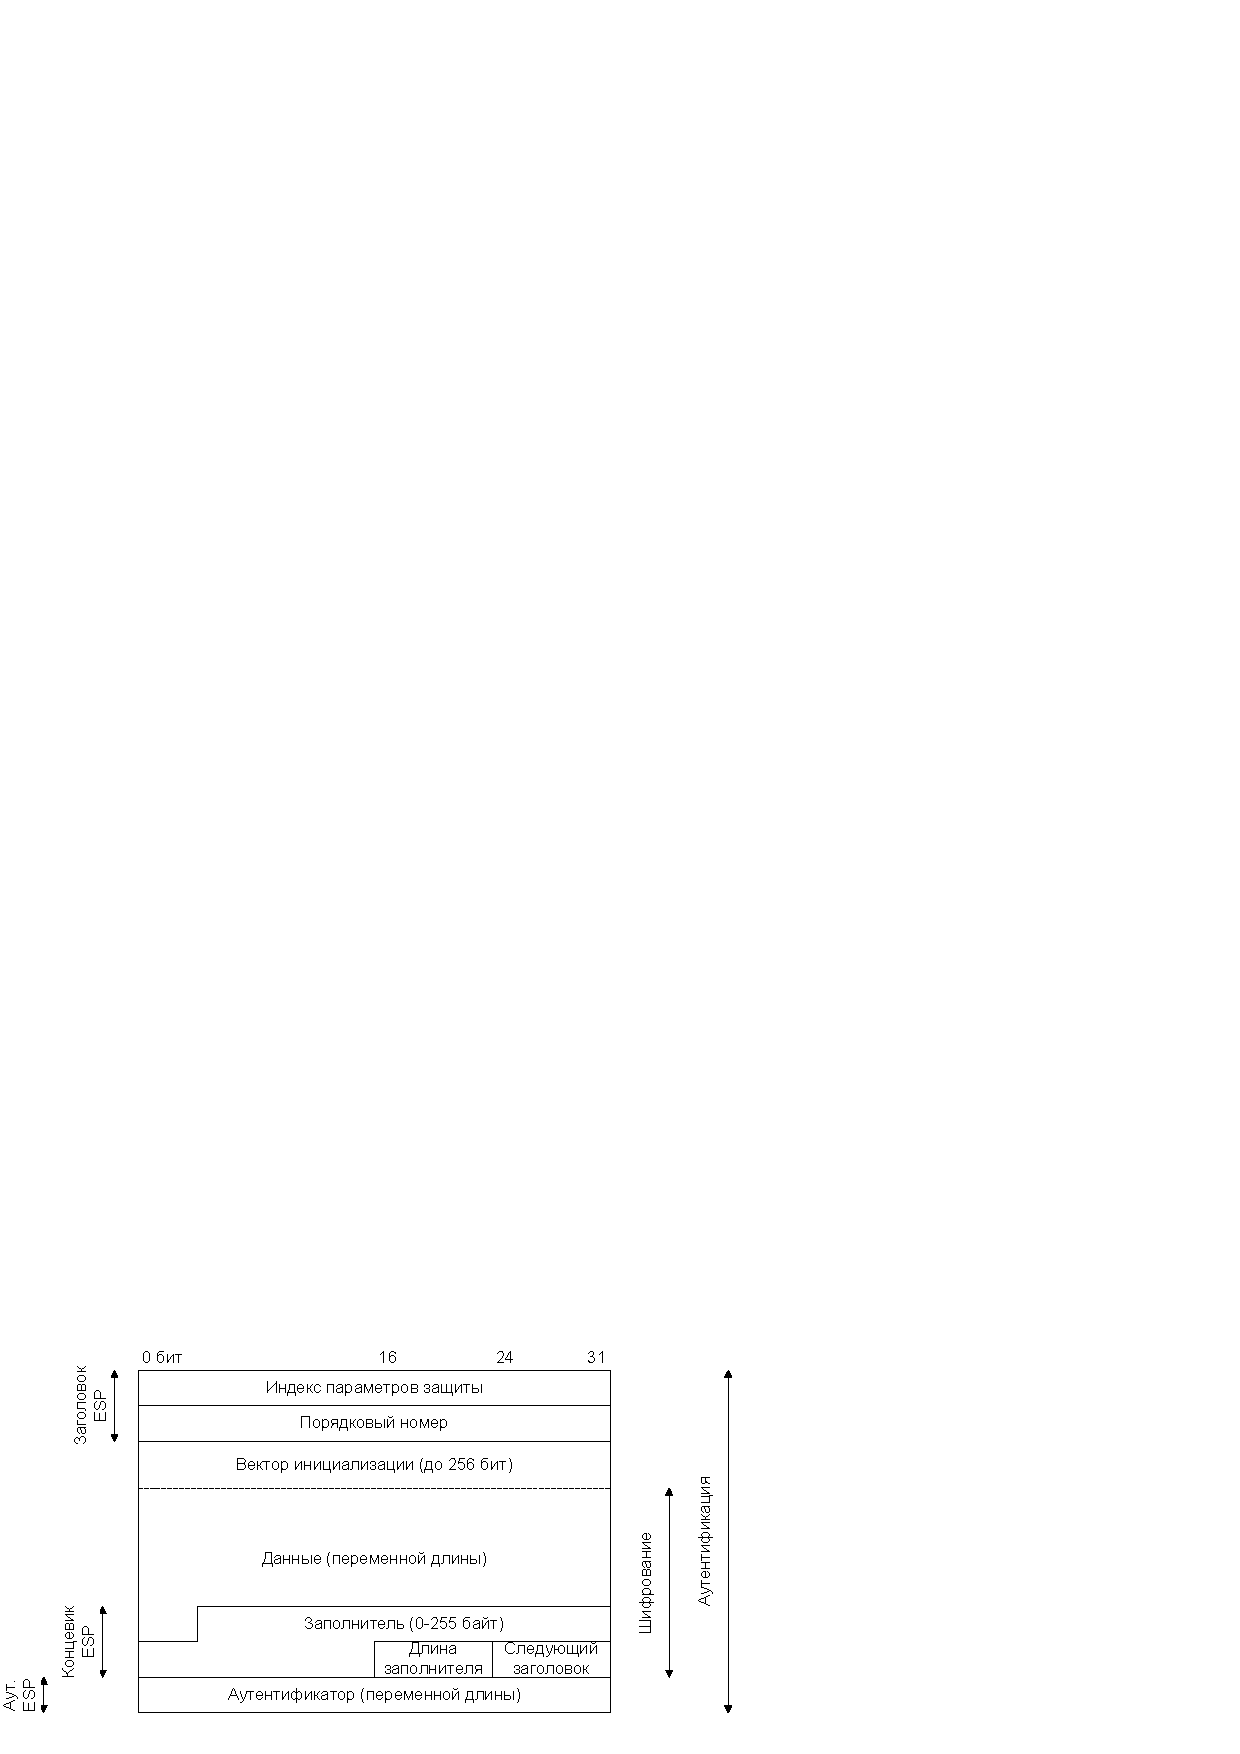
\includegraphics[width=0.9\textwidth]{pic/ipsec-esp}
	\caption{Формат ESP-пакета\label{fig:ipsec-esp}}
\end{figure}

Шифрование вложенных данных производится в режиме CBC алгоритмом AES на ключе $Ke'$ с псевдослучайным вектором инициализации IV, вставленным перед зашифрованными данными.

Аутентификатор сообщения определяется как усечённое до 96 бит значение $\HMAC(Ka', m)$, вычисленное стандартным способом.

На рис.~\ref{fig:ipsec-esp-modes} показано применение протокола в транспортном и туннельном режимах.

\begin{figure}[!ht]
	\centering
	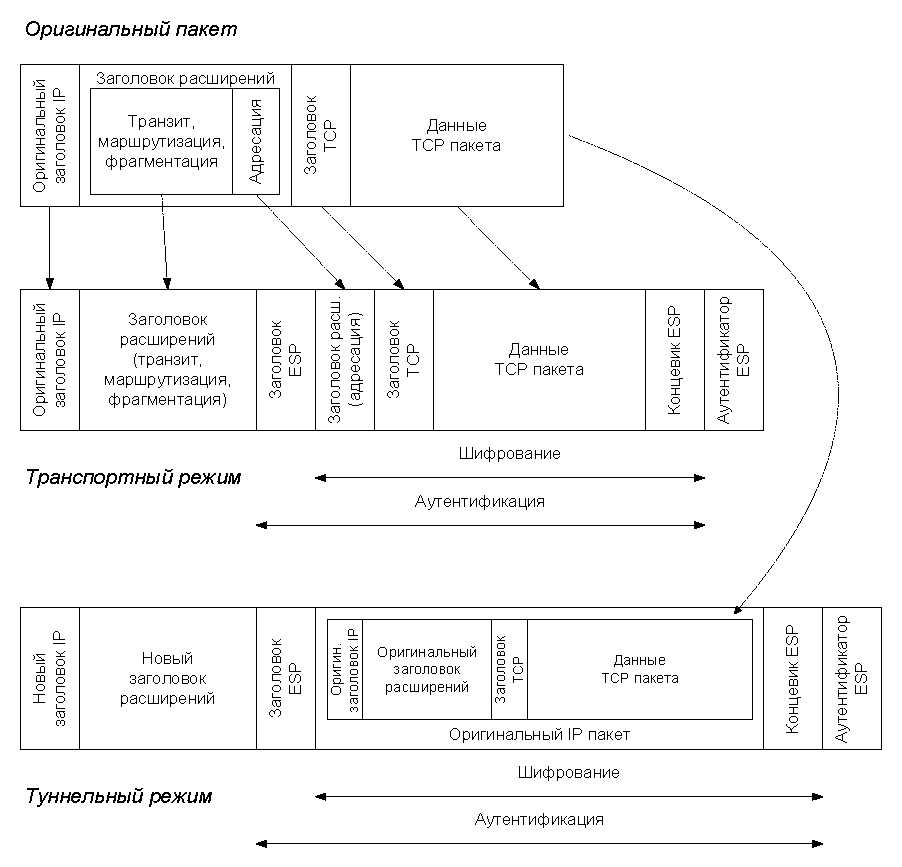
\includegraphics[width=0.9\textwidth]{pic/ipsec-esp-modes}
	\caption{Применение ESP протокола к пакету IPv6\label{fig:ipsec-esp-modes}}
\end{figure}


\subsection{Протокол аутентификации AH}

Протокол AH определяет аутентификацию всего IP-пакета в формате, показанном на рис.~\ref{fig:ipsec-ah}.

\begin{figure}[!ht]
	\centering
	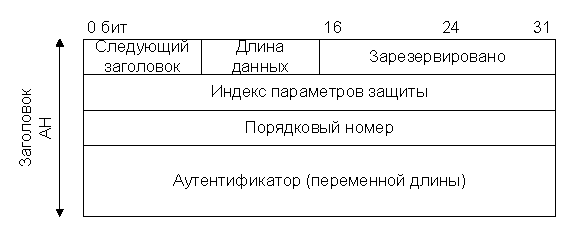
\includegraphics[width=0.7\textwidth]{pic/ipsec-ah}
	\caption{Заголовок AH пакета\label{fig:ipsec-ah}}
\end{figure}

Аутентификатор сообщения определяется так же, как и в протоколе ESP -- усечённое до 96 бит значение $\HMAC(Ka', m)$, вычисленное стандартным способом.

На рис.~\ref{fig:ipsec-ah-modes} показано применение протокола в транспортном и туннельном режимах.

\begin{figure}[!ht]
	\centering
	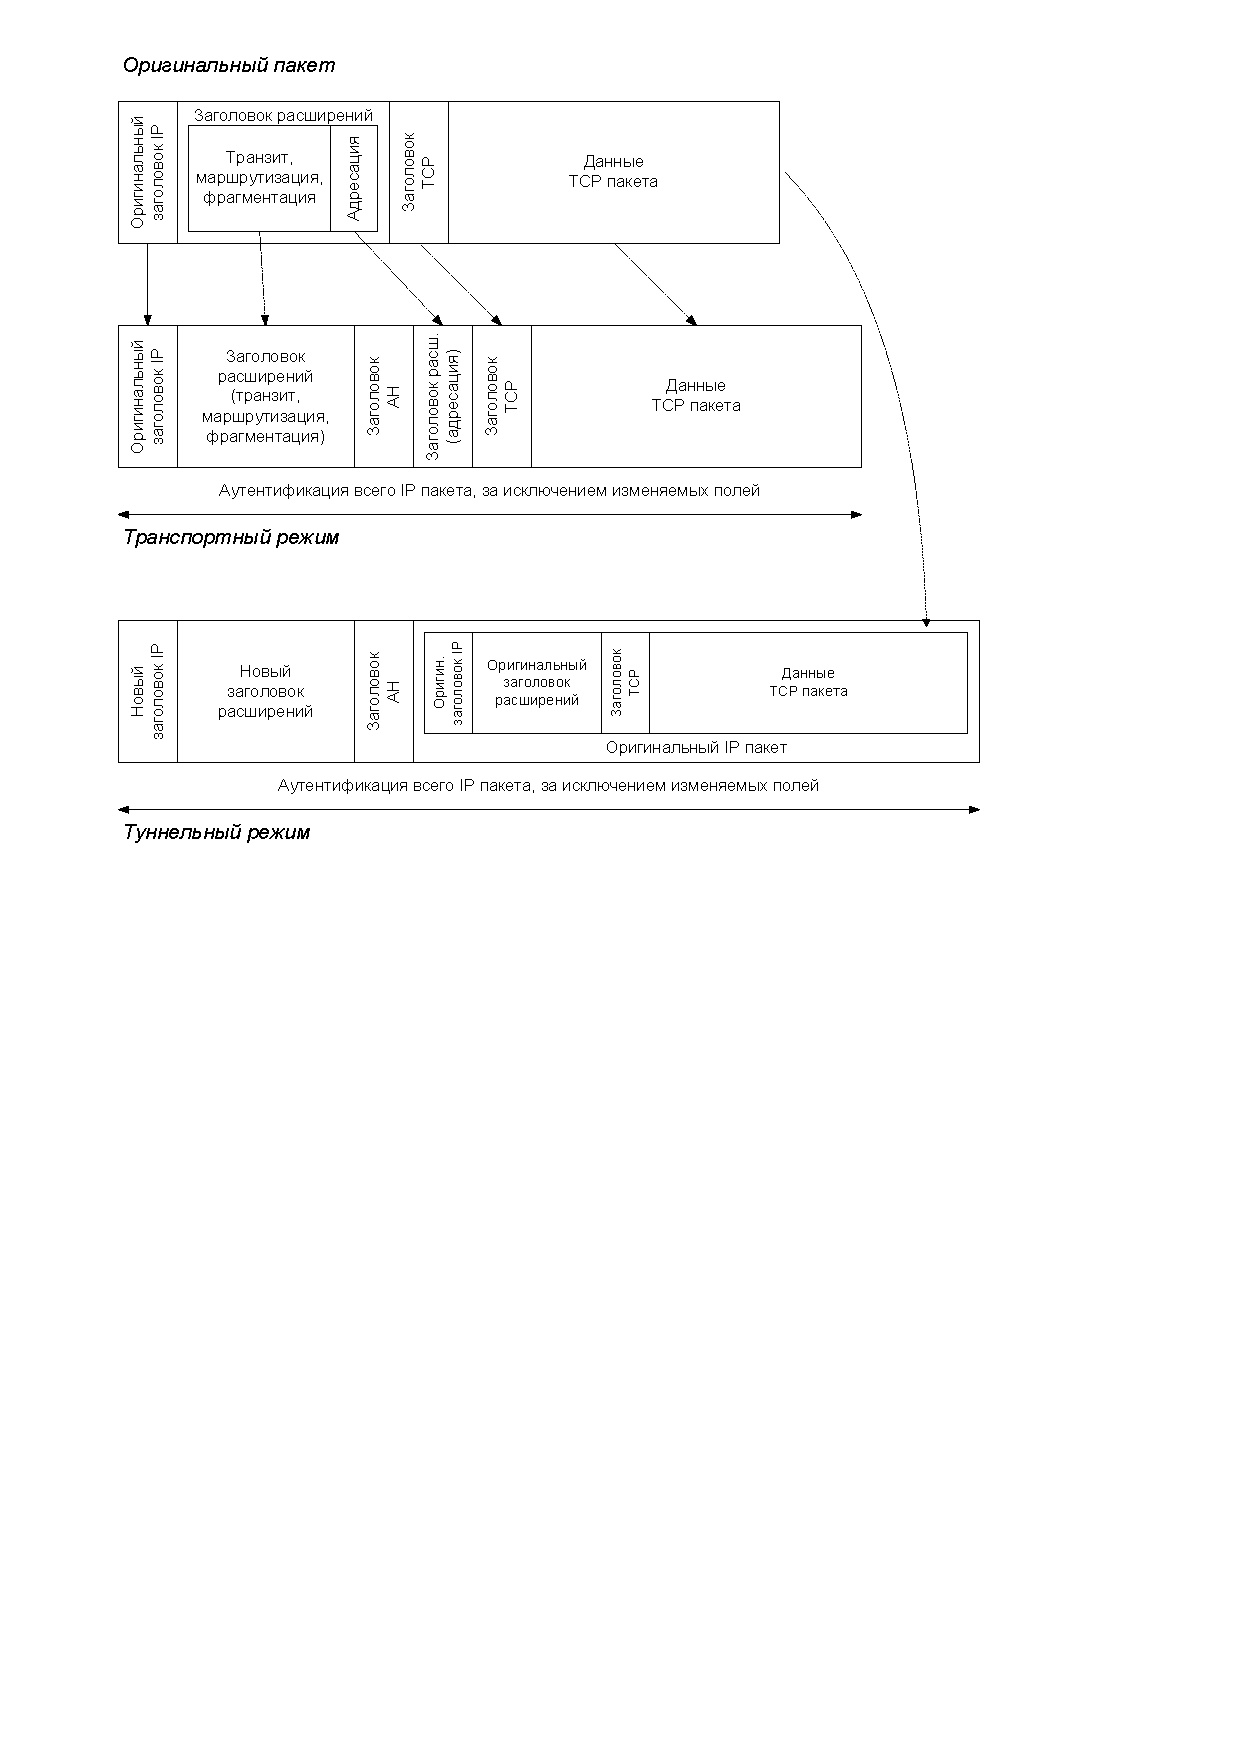
\includegraphics[width=0.9\textwidth]{pic/ipsec-ah-modes}
	\caption{Применение протокола AH к пакету IPv6\label{fig:ipsec-ah-modes}}
\end{figure}

\index{протокол!IPsec|)}

\section[Защита персональных данных в мобильной связи]{Защита персональных данных в \protect\\ мобильной связи}

\subsection{GSM (2G)}
\selectlanguage{russian}

Регистрация телефона в сети GSM построена с участием трёх сторон: SIM-карты мобильного устройства, базовой станции и центра аутентификации. SIM-карта и центр аутентификации обладают общим секретным 128-битным ключом $K_i$. Вначале телефон сообщает базовой станции уникальный идентификатор SIM-карты IMSI открытым текстом. Базовая станция запрашивает в центре аутентификации для данного IMSI набор параметров для аутентификации. Центр генерирует псевдослучайное 128-битовое число $\textrm{RAND}$ и алгоритмами A3\index{алгоритм!A3} и A8\index{алгоритм!A8} создаёт симметричный 54-битовый ключ $K_c$ и 32-битовый аутентификатор $\textrm{RES}$. Базовая станция передаёт мобильному устройству число $\textrm{RAND}$ и ожидает результата вычисления SIM-картой числа $\textrm{XRES}$, которое должно совпасть с $\textrm{RES}$ в случае успешной аутентификации. Схема аутентификации показана на рис.~\ref{fig:gsm2}.

\begin{figure}[!ht]
	\centering
	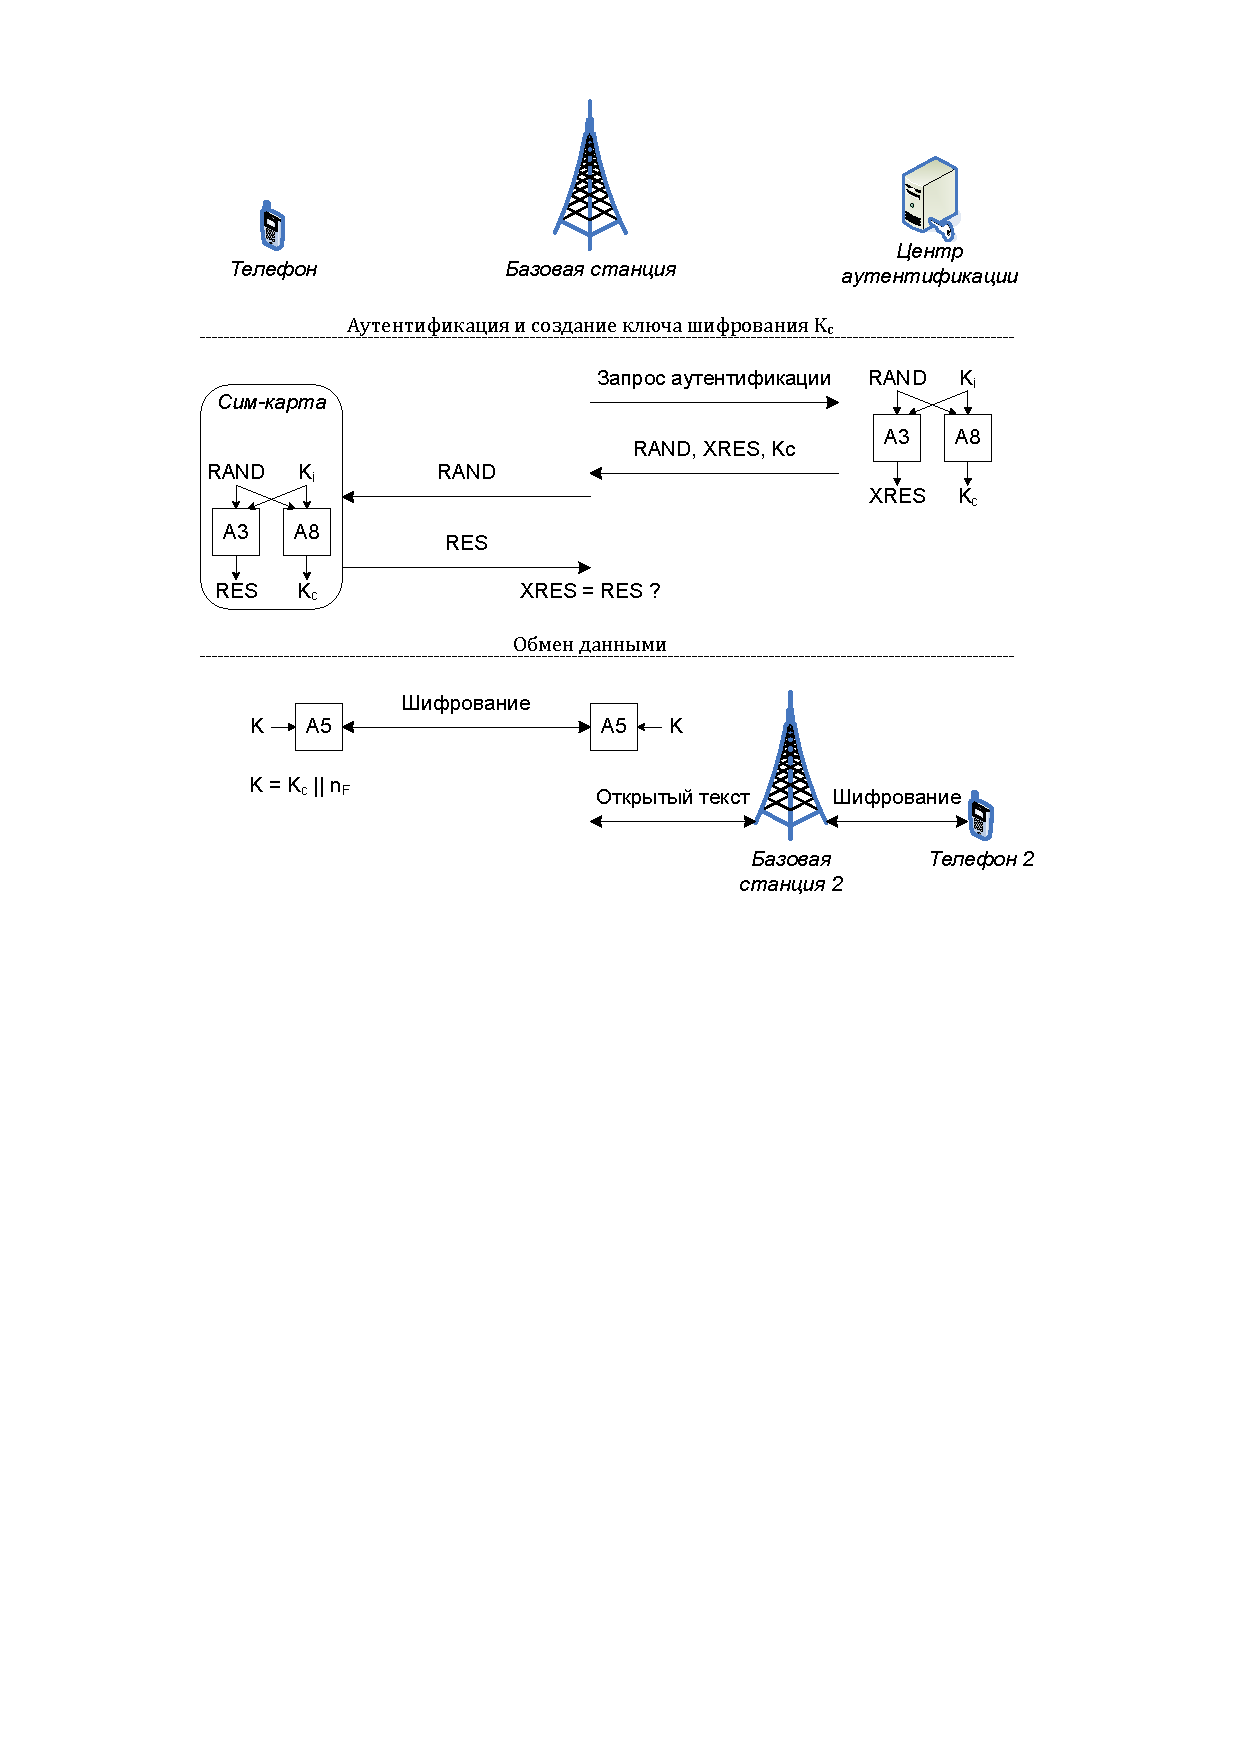
\includegraphics[width=0.85\textwidth]{pic/gsm2}
	\caption{Односторонняя аутентификация и шифрование в GSM\label{fig:gsm2}}
\end{figure}

Все вычисления для аутентификации выполняет SIM-карта. Ключ $K_c$ далее используется для создания ключа шифрования каждого фрейма $K = K_c ~\|~ n_F$, где $n_F$~--~22-битовый номер фрейма. Шифрование выполняет уже само мобильное устройство. Алгоритм шифрования фиксирован в каждой стране и выбирается из семейства алгоритмов A5\index{шифр!A5} (A5/1, A5/2, A5/3). В GSM применяется либо шифр A5/1 (используется в России), либо A5/2. Шифр A5/3 применяется уже в сети UMTS.

Аутентификация в сети GSM односторонняя. При передаче данных не используются проверка целостности и аутентификация сообщений. Передача данных между базовыми станциями происходит в открытом незашифрованном виде. Алгоритмы шифрования A5/1 и A5/2 нестойкие, количество операций для взлома A5/1~--~$2^{40}$, A5/2~--~$2^{16}$. Кроме того, длина ключа $K_c$ всего 54 бита. Передача в открытом виде уникального идентификатора IMSI позволяет однозначно определить абонента.


\subsection{UMTS (3G)}
\selectlanguage{russian}

В третьем поколении мобильных сетей, называемом UMTS, защищённость немного улучшена. Общая схема аутентификации (рис.~\ref{fig:gsm3}) осталась примерно такой же, как и в GSM. Жирным шрифтом на рисунке выделены новые добавленные элементы по сравнению с GSM.
\begin{enumerate}
    \item Производится взаимная аутентификация SIM-карты и центра аутентификации по токенам $\textrm{RES}$ и $\MAC$.
    \item Добавлены проверка целостности и аутентификация данных (имитовставка\index{имитовставка}).
    \item Используются новые алгоритмы создания ключей, шифрования и имитовставки\index{имитовставка}.
    \item Добавлены счётчики на SIM-карте $\textrm{SQN}_{\textrm{T}}$ и в центре аутентификации $\textrm{SQN}_{\textrm{Ц}}$ для защиты от атак воспроизведения. Значения увеличиваются при каждой попытке аутентификации и должны примерно совпадать.
    \item Увеличена длина ключа шифрования до 128 бит.
\end{enumerate}

\begin{figure}[!ht]
	\centering
	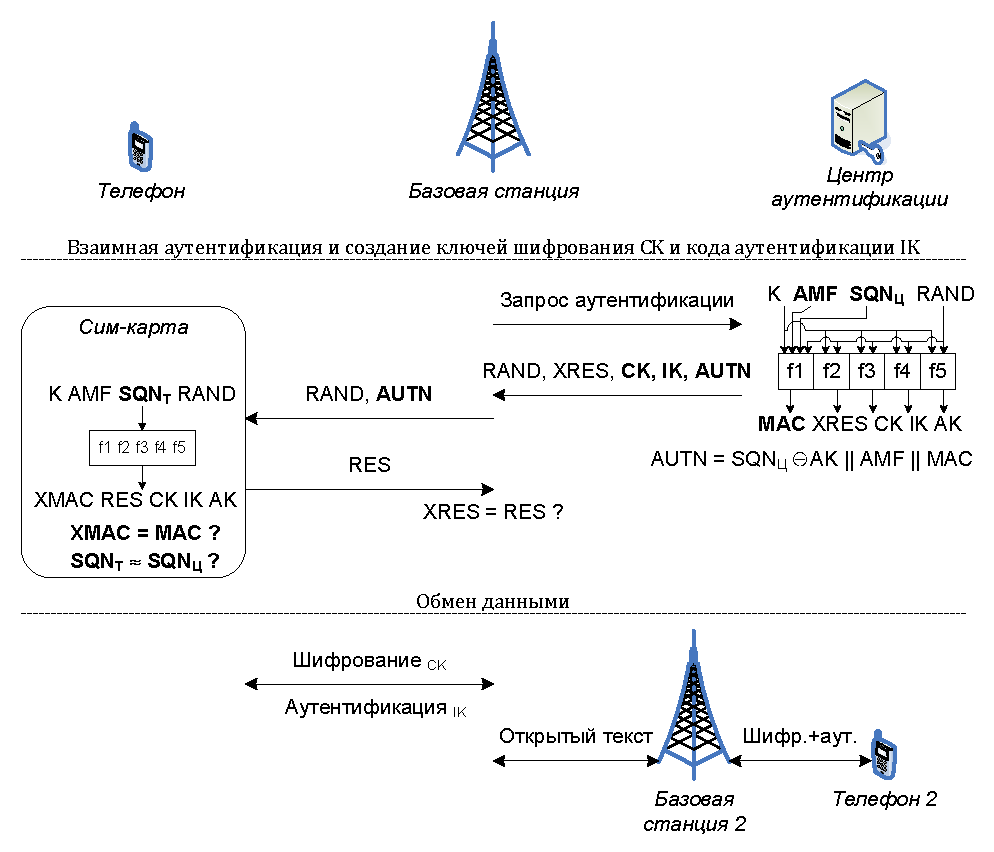
\includegraphics[width=\textwidth]{pic/gsm3}
	\caption{Взаимная аутентификация и шифрование в UMTS (3G)\label{fig:gsm3}}
\end{figure}

Обозначения на рис.~\ref{fig:gsm3} следующие:
\begin{itemize}
    \item $K$ -- общий секретный 128-битовый ключ SIM-карты и центра аутентификации;
    \item $\textrm{RAND}$ -- 128-битовое псевдослучайное число, создаваемое центром аутентификации;
    \item $\textrm{SQN}_{\textrm{T}}, \textrm{SQN}_{\textrm{Ц}}$ -- 48-битовые счётчики для защиты от атак воспроизведения;
    \item $\textrm{AMF}$ -- 16-битовое значение окна для проверки синхронизации счётчиков;
    \item $CK, IK, AK$ -- 128-битовые ключи шифрования данных $CK$, кода аутентификации данных $IK$, гаммы значения счётчика $AK$;
    \item $\MAC, \textrm{XMAC}$ -- 128-битовые аутентификаторы центра SIM-карте;
    \item $\textrm{RES}, \textrm{XRES}$ -- 128-битовые аутентификаторы SIM-карты центру;
    \item $\textrm{AUTN}$ -- вектор аутентификации.
\end{itemize}

Алгоритмы $fi$ не фиксированы стандартом и выбираются при реализациях.

Из оставшихся недостатков защиты персональных данных можно перечислить.
\begin{enumerate}
    \item Уникальный идентификатор SIM-карты IMSI по-прежнему передаётся в открытом виде, что позволяет идентифицировать абонентов по началу сеанса регистрации SIM-карты в сети.
    \item Шифрование и аутентификация производятся только между телефоном и базовой станцией, а не между двумя телефонами. Это является необходимым условием для подключения СОРМ (Система технических средств для обеспечения функций оперативно-розыскных мероприятий) по закону <<О связи>>. С другой стороны, это повышает риск нарушения конфиденциальности персональных данных.
    \item Алгоритм шифрования данных A5/3 (KASUMI) на 128-битовом ключе теоретически взламывается атакой на основе известного открытого текста для 64 MB данных с использованием 1 GiB памяти $2^{32}$ операциями (2 часа на обычном ПК).
\end{enumerate}


%\section{Беспроводная сеть Wi-Fi}
%\subsection{WPA-PSK2, 802.11n, Radix?}
%\subsection{Wimax 802.16(?)}

\chapter{Аутентификация пользователя}


\section{Многофакторная аутентификация}

Для защищённых приложений применяется \emph{многофакторная} аутентификация одновременно по факторам различной природы:
\begin{enumerate}
    \item Свойство, которым обладает субъект. Например: биометрия, природные уникальные отличия (лицо, радужная оболочка глаз, папиллярные узоры, последовательность ДНК).
    \item Знание -- информация, которую знает субъект. Например: пароль, PIN (Personal Identification Number).
    \item Владение -- вещь, которой обладает субъект. Например: электронная или магнитная карта, флэш-память.
%    \item Факторы присвоения. Например, номер машины, RFID-метка.
\end{enumerate}

В обычных массовых приложениях из-за удобства использования применяется аутентификация только по \emph{паролю}\index{пароль}, который является общим секретом пользователя и информационной системы. Биометрическая аутентификация по отпечаткам пальцев применяется существенно реже. Как правило, аутентификация по отпечаткам пальцев является дополнительным, а не вторым обязательным фактором (тоже из-за удобства её использования).

%Так же явно или неявно используется аутентификация по факторам:
%\begin{enumerate}
%    \item Социальная сеть. Доверие к индивидууму в личном или интернет общении, на основании общих связей.
%    \item Географическое положение. Например, для проверки оплаты товаров по кредитной карте.
%    \item Время. Доступ к сервисам или местам только в определённое время.
%    \item И др.
%\end{enumerate}


\section[Энтропия и криптостойкость паролей]{Энтропия и криптостойкость \protect\\ паролей}

Стандартный набор символов паролей, которые можно набрать на клавиатуре, используя английские буквы и небуквенные символы, состоит из $D=94$ символов. При длине пароля $L$ символов и предположении равновероятного использования символов энтропия паролей равна
    \[ H = L \log_2 D. \]

Клод Шеннон, исследуя энтропию символов английского текста, изучал вероятность успешного предсказания людьми следующего символа по первым нескольким символам слов или текста. В результате Шеннон получил оценку энтропии первого символа $s_1$ текста порядка $H(s_1) \approx 4{,}6$--$4{,}7$ бит/символ и оценки энтропий последующих символов, постепенно уменьшающиеся до $H(s_9) \approx 1{,}5$ бит/символ для 9-го символа. Энтропия для длинных текстов литературных произведений получила оценку $H(s_\infty) \approx 0{,}4$ бит/символ.

Статистические исследования баз паролей показывают, что наиболее часто используются буквы <<a>>, <<e>>, <<o>>, <<r>> и цифра <<1>>.

NIST (Национальный институт стандартов и технологий США, \langen{National Institute of Standards and Technology})  использует следующие рекомендации для оценки энтропии паролей\index{энтропия!пароля}, создаваемых людьми.
\begin{enumerate}
    \item Энтропия первого символа $H(s_1) = 4$ бит/символ.
    \item Энтропия со 2-го по 8-й символы $H(s_{i}) = 2$ бит/символ, $2 \leq i \leq 8$.
    \item Энтропия с 9-го по 20-й символы $H(s_{i}) = 1{,}5$ бит/символ, $9 \leq i \leq 20$.
    \item Энтропия с 21-го символа $H(s_{i}) = 1$ бит/символ, $i \geq 21$.
    \item Проверка композиции на использование символов разных регистров и небуквенных символов добавляет до 6-ти бит энтропии пароля.
    \item Словарная проверка на слова и часто используемые пароли добавляет до 6 бит энтропии для коротких паролей. Для 20-символьных и более длинных паролей прибавка к энтропии -- 0 бит.
\end{enumerate}

Для оценки энтропии пароля нужно сложить энтропии символов $H(s_i)$ и сделать дополнительные надбавки, если пароль удовлетворяет тестам на композицию и отсутствует в словаре.

\begin{table}[!ht]
    \caption{Оценка NIST предполагаемой энтропии паролей\label{tab:password-entropy}}
    \resizebox{\textwidth}{!}{ \begin{tabular}{|c||c|c|c||c|}
        \hline
        \multirow{2}{*}{\parbox{1.5cm}{\medskip \centering Длина пароля, символы}} & \multicolumn{3}{|c||}{\parbox{6cm}{\centering Энтропия паролей пользователей по критериям NIST}} & \multirow{2}{*}{\parbox{3cm}{\centering Энтропия случайных равновероятных паролей}} \\
        \cline{2-4}
        & \parbox{1.5cm}{\centering Без проверок} & \parbox{2cm}{\centering Словарная проверка} & \parbox{3cm}{\centering Словарная и композиционная проверка} & \\
        \hline
        4  & 10 & 14 & 16 & 26.3 \\
        6  & 14 & 20 & 23 & 39.5 \\
        8  & 18 & 24 & 30 & 52.7 \\
        10 & 21 & 26 & 32 & 65.9 \\
        12 & 24 & 28 & 34 & 79.0 \\
        16 & 30 & 32 & 38 & 105.4 \\
        20 & 36 & 36 & 42 & 131.7 \\
        24 & 40 & 40 & 46 & 158.0 \\
        30 & 46 & 46 & 52 & 197.2 \\
        40 & 56 & 56 & 62 & 263.4 \\
        \hline
    \end{tabular} }
\end{table}

В таблице~\ref{tab:password-entropy} приведена оценка NIST на величину энтропии пользовательских паролей в зависимости от их длины, и приведено сравнение с энтропией случайных паролей с равномерным распределением символов из набора в $D=94$ символов клавиатуры. Вероятное число попыток для подбора пароля составляет $O(2^H)$. Из таблицы видно, что по критериям NIST энтропия реальных паролей в 2--4 раза меньше энтропии случайных паролей с равномерным распределением символов.

\example
Оценим общее количество существующих паролей. Население Земли -- 7 млрд. Предположим, что всё население использует компьютеры и Интернет, и у каждого человека по 10 паролей. Общее количество существующих паролей -- $7 \cdot 10^{10} \approx 2^{36}$.

Имея доступ к наиболее массовым интернет-сервисам с количеством пользователей десятки и сотни миллионов, в которых пароли часто хранятся в открытом виде из-за необходимости обновления ПО и, в частности, выполнения аутентификации, мы:
\begin{enumerate}
	\item имеем базу паролей, покрывающую существенную часть пользователей; 
	\item можем статистически построить правила генерирования паролей.
\end{enumerate}

Даже если пароль хранится в защищённом виде, то при вводе пароль, как правило, в открытом виде пересылается по Интернету, и все преобразования пароля для аутентификации осуществляет интернет-сервис, а не веб-браузер. Следовательно, интернет-сервис имеет доступ к исходному паролю.
\exampleend

В 2002 г. был подобран ключ для 64-битного блочного шифра RC5 сетью персональных компьютеров \texttt{distributed.net}, выполнявших вычисления в фоновом режиме. Суммарное время вычислений всех компьютеров -- 1757 дней, было проверено 83\% пространства всех ключей. Это означает, что пароли с оценочной энтропией менее 64 бит, то есть \emph{все пароли} до 40 символов по критериям NIST, могут быть подобраны в настоящее время. Конечно, с оговорками на то, что 1) нет ограничений на количество и частоту попыток аутентификаций, 2) алгоритм генерации вероятных паролей эффективен.

Строго говоря, использование даже 40-символьного пароля для аутентификации или в качестве ключа блочного шифрования является небезопасным.


\subsubsection{Число паролей}

Приведём различные оценки числа паролей, создаваемых людьми. Чаще всего такие пароли основаны на словах или закономерностях естественного языка. В английском языке всего около $1\ 000\ 000 \approx 2^{20}$ слов, включая термины.

%http://www.springerlink.com/content/bh216312577r6w64/fulltext.pdf
%http://www.antimoon.com/forum/2004/4797.htm

Используемые слоги английского языка имеют вид V, CV, VC, CVV, VCC, CVC, CCV, CVCC, CVCCC, CCVCC, CCCVCC, где C -- согласная (consonant), V -- гласная (vowel). 70\% слогов имеют структуру VC или CVC. Общее число слогов $S = 8000 \dots 12000$. Средняя длина слога -- 3 буквы.

Предполагая равновероятное распределение всех слогов английского языка, для числа паролей из $r$ слогов получим верхнюю оценку
    \[ N_1 = S^r = 2^{13 r} \approx 2^{4.3 L_1}. \]
Средняя длина паролей составит:
    \[ L_1 \approx 3 r. \]

Теперь предположим, что пароли могут состоять только из 2--3 буквенных слогов вида CV, VC, CVV, VCC, CVC, CCV с равновероятным распределением символов. Подсчитаем число паролей $N_2$, которые могут быть построены из $r$ таких слогов. В английском алфавите число гласных букв $n_v = 10, согласных n_c = 16, n = n_v + n_c = 26$. Верхняя оценка числа $r$-слоговых паролей:
    \[ N_2 = (n_c n_v + n_v n_c + n_c n_v n_v + n_v n_c n_c + n_c n_v n_c + n_c n_c n_v)^r \approx \]
        \[ \approx \left( n_c n_v(3 n_c + n_v) \right)^r, \]
    \[ N_2 \approx \left( \frac{n^3}{2} \right)^r \approx 2^{13 r} \approx 2^{4.3 L_2}. \]
Средняя длина паролей:
    \[ L_2 = \frac{n_c n_v(2 + 2 + 3 n_v + 3 n_c + 3 n_c + 3 n_c)}{n_c n_v (1 + 1 + n_v + n_c + n_c + n_c)} \cdot r \approx 3 r. \]

Как видно, в обоих предположениях получились одинаковые оценки для числа и длины паролей.

Подсчитаем верхние оценки числа паролей из $L$ символов, предполагая равномерное распределение символов из алфавита мощностью $D$ символов: a) $D_1 = 26$ строчных букв, б) все $D_2 = 94$ печатных символа клавиатуры (латиница и небуквенные символы):
    \[ N_3 = D_1^L \approx 2^{4.7 L}, \]
    \[ N_4 = D_2^L \approx 2^{6.6 L}. \]

\begin{table}[!ht]
    \caption{Различные верхние оценки числа паролей\label{tab:password-number}}
    \resizebox{\textwidth}{!}{ \begin{tabular}{|c||c|c|c|}
        \hline
        \multirow{2}{*}{\parbox{1.5cm}{\medskip\medspace \centering Длина пароля}} & \multicolumn{3}{|c|}{Число паролей} \\
        \cline{2-4}
            & \parbox{3.5cm}{\medspace \centering На основе слоговой композиции} &
            \parbox{3cm}{\medspace\centering Алфавит $D=26$ символов} &
            \parbox{3cm}{\medspace \centering Алфавит $D=94$ символа} \\
        \hline
        \rule{0pt}{2.5ex}$6$  & $2^{26}$ & $2^{28}$ & $2^{39}$ \\
        9  & $2^{39}$ & $2^{42}$ & $2^{59}$ \\
        12 & $2^{52}$ & $2^{56}$ & $2^{79}$ \\
        15 & $2^{65}$ & $2^{71}$ & $2^{98}$ \\
        \hline
        \rule{0pt}{2.5ex} 21 & $2^{91}$ & $2^{99}$ & $2^{137}$ \\
        \hline
        \rule{0pt}{2.5ex} 39 & $2^{169}$ & $2^{183}$ & $2^{256}$ \\
        \hline
    \end{tabular} }
\end{table}

Из таблицы~\ref{tab:password-number} видно, что при доступном объёме вычислений в $2^{60}$\,--\,$2^{70}$ операций, пароли вплоть до 15-ти символов, построенные на словах, слогах, изменениях слов, вставках цифр, небольшом изменении регистров и других простейших модификациях, в настоящее время могут быть найдены полным перебором как на вычислительном кластере, так и на персональном компьютере.

Для достижения криптостойкости паролей, сравнимой со 128- или 256-битовым секретным ключом, требуется выбирать пароль из 20 и 40 символов соответственно, что, как правило, не реализуется из-за сложности запоминания и возможных ошибок при вводе.


%Подсчитаем число паролей $N_1$, которые могут могут построены из $r$ ~ 2-3 буквенных слогов: $cv, vc, ccv, cvc, vcc$, где $c$ -- согласная, $v$ -- гласная. В английском алфавите $n_v = 10, n_c = 16, n = n_v + n_c = 26$. Число паролей
%    \[ N_1 = \left( n_v n_c (1 + 1 + n_c + n_c + n_c) \right)^r \approx 3^r n_v^r n_c^{2r}. \]
%Средняя длина паролей
%    \[ L = r \left( \frac{2 + 2 + 3 n_c + 3 n_c + 3 n_c}{1 + 1 + n_c + n_c + n_c} \right) \approx 3r. \]
%
%%Учтем, что $b \leq r$ символов могут быть заглавными: $N_1 \rightarrow N_2 < N_1 \binom{L}{b} \left( \frac{n}{n_v} \right)^b$. Вставим $d$ цифр в случайные места: $N_2 \rightarrow N_3 = N_2 (10 (1 + L))^d \approx N_2 (10 L)^d$.
%%
%%Общее число паролей
%%    \[ N = N_3 = 3^r 10^r 16^{2r} \binom{3r}{b} 2.6^b \left(10 \cdot 3 r \right)^d. \]
%%
%%\begin{table}[!ht]
%%    \centering
%%    \small
%%    \begin{tabular}{|c|c|c|c|c||cr|}
%%        \hline
%%        \parbox{1.3cm}{Слогов, $r$} & \parbox{1.8cm}{Заглавных букв, $b$} & \parbox{1.5cm}{Вставок цифр, $d$} & \parbox{2.8cm}{Средняя длина пароля, $L+d$} & \parbox{3cm}{Верхняя оценка числа паролей $N$} & \multicolumn{2}{|c|}{\parbox{3.2cm}{Число всех паролей}} \\
%%        \hline
%%        $2$ & $0$ & $0$ & $6$ & $2^{26}$ & $2^{36}$ & a-z \\
%%        $2$ & $2$ & $0$ & $6$ & $2^{32}$ & $2^{48}$ & A-Z, a-z \\
%%        $2$ & $2$ & $2$ & $8$ & $2^{45}$ & $2^{48}$ & A-Z, a-z, 0-9 \\
%%        \hline
%%        $3$ & $0$ & $0$ & $9$ & $2^{39}$ & $2^{54}$ & a-z \\
%%        $3$ & $3$ & $0$ & $9$ & $2^{49}$ & $2^{54}$ & A-Z, a-z \\
%%        $3$ & $3$ & $2$ & $11$ & $2^{63}$ & $2^{65}$ & A-Z, a-z, 0-9 \\
%%        \hline
%%        $4$ & $0$ & $0$ & $12$ & $2^{52}$ & $2^{93}$ & a-z \\
%%        $4$ & $3$ & $0$ & $12$ & $2^{64}$ & $2^{186}$ & A-Z, a-z \\
%%        $4$ & $3$ & $2$ & $14$ & $2^{78}$ & $2^{222}$ & A-Z, a-z, 0-9 \\
%%        \hline
%%    \end{tabular}
%%    \caption{Сравнение верхней оценки числа паролей, построенных на слогах, со всем доступным множеством паролей.}
%%    \label{tab:password-number}
%%\end{table}
%
%Учтем, что $b$ символов в пароле могут быть взяты не из 26-символьного алфавита строчных букв, а из всего алфавита в $D=94$ печатных символа клавиатуры (латиница и небуквенные символы):
%\[
%    \begin{array}{ll}
%    b=1 & N_1 \rightarrow N_2 = \frac{n_v}{n_v+n_c} 3^r n_v^{r-1} n_c^{2r} \cdot L. \]
%
%    \[ N_1 \rightarrow N_2 < N_1 \binom{L}{b} \left( \frac{D}{n_v} \right)^b. \]
%
%
%
%Общее число паролей
%    \[ N < 3^r n_v^r n_c^{2r} \binom{L}{b} \left( \frac{D}{n_v} \right)^b = 3^r 10^r 16^{2r} \binom{3r}{b} \left( \frac{94}{10} \right)^b. \]
%
%\begin{table}[!ht]
%    \centering
%    \small
%    \begin{tabular}{|c|c|c|c||cr|}
%        \hline
%        \parbox{1.5cm}{Слогов, $r$} & \parbox{3cm}{Средняя длина пароля, $L$} & \parbox{3cm}{Символов из всего алфавита, $b$} & \parbox{3cm}{Верхняя оценка числа паролей $N$} & \multicolumn{2}{|c|}{\parbox{3.2cm}{Число всех паролей, $D^L$}} \\
%        \hline
%        \multirow{3}{*}{2} & \multirow{3}{*}{6} & $0$ & $2^{26}$ & $2^{28}$ & a-z \\
%        & & $1$ & $2^{32}$ & $2^{34}$ & A-Z, a-z \\
%        & & $3$ & $2^{40}$ & $2^{39}$ & Весь алфавит \\
%        \hline
%        \multirow{3}{*}{3} & \multirow{3}{*}{9} & $0$ & $2^{39}$ & $2^{42}$ & a-z \\
%        & & $2$ & $2^{50}$ & $2^{51}$ & A-Z, a-z \\
%        & & $4$ & $2^{59}$ & $2^{59}$ & Весь алфавит \\
%        \hline
%        \multirow{3}{*}{4} & \multirow{3}{*}{12} & $0$ & $2^{52}$ & $2^{56}$ & a-z \\
%        & & $3$ & $2^{69}$ & $2^{68}$ & A-Z, a-z \\
%        & & $6$ & $2^{81}$ & $2^{77}$ & Весь алфавит \\
%        \hline
%    \end{tabular}
%    \caption{Сравнение верхней оценки числа паролей, построенных на слогах, со всем доступным множеством паролей в алфавите из $D$ символов.}
%    \label{tab:password-number}
%\end{table}
%
%Из таблицы~\ref{tab:password-number} видно, что при доступном объёме вычислений в $2^{60 \ldots 70}$ операций, пароли вплоть до 12 символов, построенные на словах, слогах, изменениях слов, вставках цифр, небольшого изменения регистров и другой простейшей обфускации, могут быть найдены перебором на кластере (или ПК) в настоящее время.


\subsubsection{Атака для подбора паролей и ключей шифрования}

В схемах аутентификации по паролю иногда используется хэширование и хранение хэша пароля на сервере. В таких случаях применима словарная атака или атака с применением заранее вычисленных таблиц для ускорения поиска.

Для нахождения пароля, прообраза хэш-функции, или для нахождения ключа блочного шифрования по атаке с выбранным шифртекстом (для одного и того же известного открытого текста и соответствующего шифртекста) может быть применён метод перебора с балансом между памятью и временем вычислений. Самый быстрый метод радужных таблиц\index{радужные таблицы} (\langen{rainbow tables}, 2003~г., \cite{Oechslin:2003}) заранее вычисляет следующие цепочки и хранит результат в памяти.

Для нахождения пароля, прообраза хэш-функции $H$, цепочка строится как
    \[ M_0 \xrightarrow{H(M_0)} h_0 \xrightarrow{R_0(h_0)} M_1 \ldots M_t \xrightarrow{H(M_t)} h_t \xrightarrow{R_t(h_t)} M_{t+1}, \]
где $R_i(h)$ -- функция редуцирования, преобразования хэша в пароль для следующего хэширования.

Для нахождения ключа блочного шифрования для одного и того же известного открытого текста $M$ таблица строится как
    \[ K_0 \xrightarrow{E_{K_0}(M)} c_0 \xrightarrow{R_0(c_0)} K_1 \ldots K_t \xrightarrow{E_{K_t}(M)} c_t \xrightarrow{R_t(c_t)} K_{t+1}, \]
где $R_i(c)$ -- функция редуцирования, преобразования шифртекста в новый ключ.

Функция редуцирования $R_i$ зависит от номера итерации, чтобы избежать дублирующихся подцепочек, которые возникают в случае коллизий между значениями в разных цепочках в разных итерациях, если $R$ постоянна. Радужная таблица размера $(m \times 2)$ состоит из строк $(M_{0,j}, M_{t+1,j})$ или $(K_{0,j}, K_{t+1,j})$, вычисленных для разных значений стартовых паролей $M_{0,j}$ или $K_{0,j}$ соответственно.

Опишем атаку на примере нахождения прообраза $\overline{M}$ хэша $\overline{h} = H(\overline{M})$. На первой итерации исходный хэш $\overline{h}$ редуцируется в сообщение $\overline{h} \xrightarrow{R_t(\overline{h})} \overline{M}_{t+1} $ и сравнивается со всеми значениями последнего столбца $M_{t+1,j}$ таблицы. Если нет совпадения, переходим ко второй итерации. Хэш $\overline{h}$ дважды редуцируется в сообщение $\overline{h} \xrightarrow{R_{t-1}(\overline{h})} \overline{M}_t \xrightarrow{H(\overline{M}_t)} \overline{h}_t \xrightarrow{R_t(\overline{h}_t)} \overline{M}_{t+1}$ и сравнивается со всеми значениями последнего столбца $M_{t+1,j}$ таблицы. Если не совпало, то переходим к третьей итерации и~т.\,д. Если для $r$-кратного редуцирования сообщение $\overline{M}_{t+1}$ содержится в таблице во втором столбце, то из совпавшей строки берётся $M_{0,j}$, и вся цепочка пробегается заново для поиска искомого сообщения $\overline{M}: ~ \overline{h} = H(\overline{M})$.

Найдём вероятность нахождения пароля в таблице. Пусть мощность множества всех паролей равна $N$. Изначально в столбце $M_{0,j}$ содержится $m_0 = m$ различных паролей. Предполагая наличие случайного отображения с пересечениями паролей $M_{0,j} \rightarrow M_{1,j}$, в $M_{1,j}$ будет $m_1$ различных паролей. Согласно задаче о размещении,
\[
    m_{i+1} = N \left( 1 - \left( 1 - \frac{1}{N} \right)^{m_i} \right) \approx N \left( 1 - e^{-\frac{m_i}{N}} \right).
\]
Вероятность нахождения пароля:
\[
    P = 1 - \prod \limits_{i=1}^t \left( 1 - \frac{m_i}{N} \right).
\]

Чем больше таблица из $m$ строк, тем больше шансов найти пароль или ключ, выполнив в наихудшем случае   $O \left( m \frac{t(t+1)}{2} \right)$ операций.

Примеры применения атаки на хэш-функциях $\textrm{MD5}$\index{хэш-функция!MD5}, $\textrm{LM} \sim \textrm{DES}_{\textrm{Password}} (\textrm{const})$ приведены в таблице~\ref{tab:rainbow-tables}.

\begin{table}[!ht]
    \centering
    \caption{Атаки на радужных таблицах на \emph{одном} ПК\label{tab:rainbow-tables}}
    \resizebox{\textwidth}{!}{ \begin{tabular}{|c|c|c|c|c|c|c|}
        \hline
        \multirow{2}{*}{\parbox{1.0cm}{\medskip\medskip \centering Длина, биты}} & \multicolumn{3}{|c|}{\parbox{4.3cm}{\medspace\centering Пароль или ключ}} &
            \multicolumn{3}{|c|}{\parbox{4.33cm}{\medspace\centering Радужная таблица}} \\
        \cline{2-7}
        & \parbox{1.0cm}{\centering Длина,\\ симв.} & \parbox{1.7cm}{\centering Множество} & \parbox{1.7cm}{\centering Мощность} &
            \parbox{1cm}{\centering Объём} & \parbox{2.23cm}{\medspace \centering Время вычисления таблиц} & \parbox{1.1cm}{\centering Время поиска} \\
        \hline \hline
        \multicolumn{7}{|c|}{Хэш LM} \\
        \hline
        \rule{0pt}{2.5ex}\multirow{3}{*}{$2 \times 56$} & \multirow{3}{*}{14} &
            A--Z & $2^{33}$ & 610 MB &  & 6 с \\
        & & A--Z, 0-9 & $2^{36}$ & 3 GB &  & 15 с \\
        & & все & $2^{43}$ & 64 GB & \parbox{2.23cm}{несколько лет} & 7 мин \\
        \hline \hline
        \multicolumn{7}{|c|}{Хэш MD5} \\
        \hline
        \rule{0pt}{2.5ex} 128 & 8 & A-Z, 0-9 & $2^{41}$ & 36 GiB & - & 4 мин \\
        \hline
    \end{tabular} }
\end{table}

\section{Аутентификация по паролю}

Из-за малой энтропии пользовательских паролей во всех системах регистрации и аутентификации пользователей применяется специальная политика безопасности. Типичные минимальные требования:
\begin{enumerate}
    \item Длина пароля от 8 символов. Использование разных регистров и небуквенных символов в паролях. Запрет паролей из словаря или часто используемых паролей. Запрет паролей в виде дат, номеров машин и других номеров.
    \item Ограниченное время действия пароля. Обязательная смена пароля по истечении срока действия.
    \item Блокирование возможности аутентификации после нескольких неудачных попыток. Ограниченное число актов аутентификации в единицу времени. Временная задержка перед выдачей результата аутентификации.
\end{enumerate}

Дополнительные меры предосторожности для пользователей:
\begin{enumerate}
    \item Не использовать одинаковые или похожие пароли для разных систем, таких как электронная почта, вход в ОС, электронная платёжная система, форумы, социальные сети. Пароль часто передаётся в открытом виде по сети. Пароль доступен администратору системы, возможны утечки конфиденциальной информации с серверов. Поэтому следует стараться выбирать случайные стойкие пароли.
    \item Не записывать пароли. Никому не сообщать пароль, даже администратору. Не передавать пароли по почте, телефону, Интернету и~т.\,д.
    \item Не использовать одну и ту же учётную запись для разных пользователей, даже в виде исключения.
    \item Всегда блокировать компьютер, когда пользователь отлучается от него, даже на короткое время.
\end{enumerate}

\input{os_passwords}

\input{http_auth}

\chapter{Программные уязвимости}

\input{security_models}

\input{os_access_controls}

\section{Виды программных уязвимостей}

\emph{Вирусом} называется самовоспроизводящаяся часть кода (подпрограмма)\index{вирус}, которая встраивается в носители (другие программы) для своего исполнения и распространения. Вирус не может исполняться и передаваться без своего носителя.

\emph{Червём} называется самовоспроизводящаяся отдельная (под)программа\index{червь}, которая может исполняться и распространяться самостоятельно, не используя программу-носитель.

Первой вехой в изучении компьютерных вирусов можно назвать 1949 год, когда Джон фон Нейман прочёл курс лекций в Университете Иллинойса под названием <<Теория самовоспроизводящихся машин>> (изданы в 1966~\cite{Neumann:1966}, переведены на русский язык издательством <<Мир>> в 1971 году~\cite{Neumann:1971}), в котором ввёл понятие самовоспроизводящихся механических машин. Первым сетевым вирусом считается вирус Creeper 1971 г., распространявшийся в сети ARPANET, предшественнице Интернета. Для его уничтожения был создан первый антивирус Reaper, который находил и уничтожал Creeper.

Первый червь для Интернета, червь Морриса, 1988 г., уже использовал \emph{смешанные} атаки\index{атака!смешанная} для заражения UNIX машин~\cite{EichinRochlis:1988, Spafford:1989}. Сначала программа получала доступ к удалённому запуску команд, эксплуатируя уязвимости в сервисах \texttt{sendmail}, \texttt{finger} (с использованием атаки на переполнение буфера) или \texttt{rsh}. Далее, с помощью механизма подбора паролей червь получал доступ к локальным аккаунтам пользователей:
\begin{itemize}
    \item получение доступа к учётным записям с очевидными паролями:
		\begin{itemize}
			\item без пароля вообще;
			\item имя аккаунта в качестве пароля;
			\item имя аккаунта в качестве пароля, повторённое дважды;
			\item использование <<ника>> (\langen{nickname});
			\item фамилия (\langen{last name, family name});
			\item фамилия, записанная задом наперёд;
		\end{itemize}
		\item перебор паролей на основе встроенного словаря из 432 слов;
		\item перебор паролей на основе системного словаря \texttt{/usr/dict/words}.
\end{itemize}

\emph{Программной уязвимостью}\index{программная уязвимость} называется свойство программы, позволяющее нарушить её работу. Программные уязвимости могут приводить к отказу в обслуживании (Denial of Service, DoS-атака)\index{атака!отказ в обслуживании}, утечке и изменению данных, появлению и распространению вирусов и червей.

Одной из распространённых атак для заражения персональных компьютеров является переполнение буфера в стеке. В интернет-сервисах наиболее распространённой программной уязвимостью в настоящее время является межсайтовый скриптинг (Cross-Site Scripting, XSS-атака)\index{атака!XSS}.

Наиболее распространённые программные уязвимости можно разделить на классы:
\begin{enumerate}
    \item Переполнение буфера -- копирование в буфер данных большего размера, чем длина выделенного буфера. Буфером может быть контейнер текстовой строки, массив, динамически выделяемая память и~т.\,д. Переполнение становится возможным вследствие либо отсутствия контроля над длиной копируемых данных, либо из-за ошибок в коде. Типичная ошибка -- разница в 1 байт между размерами буфера и данных при сравнении.
    \item Некорректная обработка (парсинг) данных, введённых пользователем, является причиной большинства программных уязвимостей в веб-приложениях. Под обработкой понимаются:
        \begin{enumerate}
            \item проверка на допустимые значения и тип (числовые поля не должны содержать строки и~т.\,д.);
            \item фильтрация и экранирование специальных символов, имеющих значения в скриптовых языках или применяющихся для перекодирования из одной текстовой кодировки в другую. Примеры символов: \texttt{\textbackslash}, \texttt{\%}, \texttt{<}, \texttt{>}, \texttt{"}, \texttt{'};
            \item фильтрация ключевых слов языков разметки и скриптов. Примеры: \texttt{script}, \texttt{JavaScript};
            \item перекодирование различными кодировками при парсинге. Распространённый способ обхода системы контроля парсинга данных состоит в однократном или множественном последовательном кодировании текстовых данных в шестнадцатеричные кодировки \texttt{\%NN} ASCII и UTF-8. Например, браузер или веб-приложения производят $n$-кратное перекодирование, в то время как система контроля делает $k$-кратное перекодирование, $0 \leq k < n$, и, следовательно, пропускает закодированные запрещённые символы и слова.
        \end{enumerate}
    \item Некорректное использование функций. Например, \texttt{printf(s)} может привести к уязвимости записи в память по указанному адресу. Если злоумышленник вместо обычной текстовой строки введёт в качестве \texttt{s "текст некоторой длины\%n"}, то функция \texttt{printf}, ожидающая первым аргументом строку формата \texttt{fmt}, обнаружив \texttt{\%n}, возьмёт значение из ячеек памяти, находящихся перед ячейками с указателем на текстовую строку (устройство стека описано далее), и запишет в память по адресу, равному считанному значению, количество выведенных символов на печать функцией \texttt{printf}.
\end{enumerate}


\input{stack_overflow}

\input{xss}

\input{sql-injections}

%\chapter{Послесловие}
%Это должно быть что-то в виде заключения, объяснения, почему именно эти темы выбраны, насколько актуален материал с теоретической и практической точки зрения.


\appendix
\renewcommand{\thechapter}{\Asbuk{chapter}} % использование русских букв для нумерации приложений

\chapter{Математическое приложение}\label{chap:discrete-math}

\section{Общие определения}

Выражением $\Mod n$ обозначается вычисление остатка от деления произвольного целого числа на целое число $n$. В полиномиальной арифметике эта операция означает вычисление остатка от деления многочленов.
%далее будем обозначать целые числа или операции с целыми числами, взятыми \emph{по модулю}\index{модуль} целого числа $n$ (остаток от целочисленного деления). Примеры выражений:
    \[ a\mod n, \]
    \[ (a + b)\cdot c\mod n. \]
Равенство
    \[ a = b \mod n \]
означает, что выражения $a$ и $b$ равны (говорят также <<сравнимы>>, <<эквивалентны>>) по модулю $n$.

Множество
    \[ \{ 0, 1, 2, 3, \dots, n-1 \mod n\} \]
состоит из $n$ элементов, где каждый элемент $i$ представляет все целые числа, сравнимые с $i$ по модулю $n$.

Наибольший общий делитель (НОД) двух чисел $a,b$ обозначается $\gcd(a,b)$ (\textit{greatest common divisor}).

Два числа $a,b$ называются взаимно простыми, если они не имеют общих делителей, кроме 1, то есть $\gcd(a,b) = 1$.

Выражение $a \mid b$ означает, что $a$ делит $b$.

\section{Парадокс дней рождения}\label{section-birthday-padradox}
\selectlanguage{russian}

Парадокс дней рождения\index{парадокс дней рождения} связан с контринтуитивным ответом на следующую задачу: какой должен быть минимальный размер группы, чтобы вероятность совпадения дней рождения хотя бы у пары человек из этой группы была больше $1 / 2$? Первый возникающий в голове вариант ответа <<183 человека>> (то есть $\left\lceil 365 / 2 \right\rceil$) является неверным.

Найдём вероятность $P(n)$ того, что в группе из $n$ человек хотя бы двое имеют дни рождения в один день года. Вероятность того, что $n$ человек ($n < N = 365$) не имеют общего дня рождения, есть
\[
    \bar{P}(n) = 1 \cdot \left( 1 - \frac{1}{N} \right) \cdot \left(1 - \frac{2}{N} \right)\cdot \dots \cdot  \left( 1 - \frac{n-1}{N} \right) = \prod\limits_{i=0}^{n-1} \left( 1 - \frac{i}{N} \right).
\]

Аппроксимируя $1-x \leq \exp({-x})$, находим
    \[ \bar{P}(n) \approx \prod\limits_{i=0}^{n-1} \exp\left(-\frac{i}{N}\right) = \exp\left(-\frac{n(n-1)}{2} \cdot \frac{1}{N}\right) \approx \exp\left(-\frac{n^2}{2} \cdot \frac{1}{N}\right). \]

Вероятность того, что хотя бы 2 человека из $n$ имеют общий день рождения, есть
    \[ P(n) = 1 - \bar{P}(n) \approx 1 -  \exp\left(-\frac{n^2}{2} \cdot \frac{1}{N}\right). \]

Кроме того, найдём минимальный размер группы, в которой дни рождения совпадают хотя бы у двоих с вероятностью не менее $1 / 2$. То есть найдём такое число $n_{1/2}$, чтобы выполнялось условие $P(n_{1/2}) \geq \frac{1}{2}$. Подставляя это значение в формулу для вероятности, получим $\frac{1}{2} \geq \exp\left(-\frac{n_{1/2}^2}{2} \cdot \frac{1}{N}\right)$. Следовательно,
	\[n_{1/2} \geq \sqrt{2 \ln 2 \cdot N} \approx 1,18 \sqrt{ N } \approx 22,5.\]
В криптографии при оценках стойкости алгоритмов часто опускают коэффициент $\sqrt{2 \ln 2}$, считая ответом на задачу <<округлённое>> значение $\sqrt{ N }$. Например, оценку числа операций хэширования для поиска коллизии идеальной криптографической хэш-функции с размером выхода $k$ бит часто записывают как $2^{k/2}$.


\section{Группы}\label{section-groups}
\selectlanguage{russian}

\subsection{Свойства групп}

\emph{Группой}\index{группа} называется множество $\Gr$, на котором задана бинарная операция <<$\circ$>>, удовлетворяющая следующим аксиомам:
\begin{itemize}
    \item замкнутость:
        \[ \forall a,b \in \Gr ~ a \circ b = c \in \Gr; \]
    \item ассоциативность:
        \[ \forall a,b,c \in \Gr ~ (a \circ b) \circ c = a \circ (b \circ c); \]
    \item существование единичного элемента:
        \[ \exists ~ e \in \Gr: \forall a \in \Gr ~ e \circ a = a \circ e = a; \]
    \item существование обратного элемента:
        \[ \forall a \in \Gr ~ \exists ~ b \in \Gr: a \circ b = b \circ a = e. \]
\end{itemize}
Если
    \[ \forall a,b \in \Gr ~ a \circ b = b \circ a, \]
то такую группу называют \emph{коммутативной} (или \emph{абелевой}).

Если операция в группе задана как умножение <<$\cdot$>>, то группа называется \emph{мультипликативной}. Для мультипликативной группы будем использовать следующие соглашения об обозначениях:
\begin{itemize}
	\item нейтральный элемент: $e \equiv 1$;
	\item обратный элемент: $a^{-1}$;
	\item повторение операции над одним аргументом $k$ раз (возведение в степень k): $a^k$.
\end{itemize}

Если операция задана как сложение <<$+$>>, то группа называется \emph{аддитивной}. Соглашение об обозначениях для аддитивной группы:
\begin{itemize}
	\item нейтральный элемент: $e \equiv 0$;
	\item обратный элемент: $-a$;
	\item повторение операции над одним аргументом $k$ раз (умножение на k): $ka$.
\end{itemize}

Подмножество группы, удовлетворяющее аксиомам группы, называется \emph{подгруппой}\index{подгруппа}.

\emph{Порядком} $|\Gr|$ \emph{группы}\index{порядок группы} $\Gr$ называется число элементов в группе. Пусть группа мультипликативная. Для любого элемента $a \in \Gr$ выполняется $a^{|\Gr|} = 1$.

\emph{Порядком элемента} $a$ называется минимальное натуральное число
    \[ \ord(a): a^{\ord(a)} = 1. \]

 Порядок элемента, согласно теореме Лагранжа\index{теорема!Лагранжа}, делит порядок группы:
    \[ \ord(a) \mid \left|\Gr\right|. \]


\subsection{Циклические группы}

\emph{Генератором} $g \in \Gr$ называется элемент, \emph{порождающий} всю группу\index{генератор группы}:
    \[ \Gr = \{g, g^2, g^3, \ldots, g^{|\Gr|} = 1\}. \]

Группа, в которой существует генератор, называется \emph{циклической}\index{группа!циклическая}.

Если конечная группа не циклическая, то в ней существуют циклические подгруппы, порождённые всеми элементами. Любой элемент $a$ группы порождает либо циклическую \emph{подгруппу}
    \[ \{ a, a^2, a^3, \dots, a^{\ord(a)} = 1 \} \]
порядка $\ord(a)$, если порядок элемента $\ord(a) < |\Gr|$, либо \emph{всю группу}
    \[ \Gr = \{ a, a^2, a^3, \dots, a^{|\Gr|} = 1 \}, \]
если порядок элемента равен порядку группы $\ord(a) = |\Gr|$. Порядок любой подгруппы, как и порядок элемента, делит порядок всей группы.

Представим циклическую группу через генератор $g$ как
    \[ \Gr = \{g, g^2, \ldots, g^{|\Gr|} = 1\} \]
и каждый элемент $g^i$ возведём в степени $1, 2, \ldots, |\Gr|$. Тогда
\begin{itemize}
    \item элементы $g^i$, для которых число $i$ взаимно просто с $|\Gr|$, породят снова всю группу
            \[ \Gr = \{ g^i, g^{2i}, g^{3i}, \dots, g^{|\Gr| i} = 1 \}, \]
        так как степени $\{i, 2i, 3i, \dots, |\Gr| i \}$ по модулю $|\Gr|$ образуют перестановку чисел $\{1, 2, 3, \dots, |\Gr|\}$; следовательно, $g^i$ -- тоже генератор, число таких чисел $i$ равно по определению функции Эйлера $\varphi(|\Gr|)$ ($\varphi(n)$ -- количество взаимно простых с $n$ целых чисел в диапазоне $[1,n-1]$);
    \item элементы $g^i$, для которых $i$ имеют общие делители
            \[ d_i = \gcd(i, |\Gr|) \neq 1 \]
        c $|\Gr|$, породят подгруппы
            \[ \{ g^i, g^{2i}, g^{3i}, \dots, g^{\frac{i}{d_i} |\Gr|} = 1\}, \]
        так как степень последнего элемента кратна $|\Gr|$; следовательно, такие $g^i$ образуют циклические подгруппы порядка $d_i$.
\end{itemize}

Из предыдущего утверждения следует, что число генераторов в циклической группе равно
    \[ \varphi(|\Gr|). \]

Для проверки, является ли элемент генератором всей группы, требуется знать разложение порядка группы $|\Gr|$ на множители. Далее элемент возводится в степени, равные всем делителям порядка группы, и сравнивается с единичным элементом $e$. Если ни одна из степеней не равна $e$, то этот элемент является примитивным элементом или генератором группы. В противном случае элемент будет генератором какой-либо подгруппы.

Задача разложения числа на множители является трудной для вычисления. На сложности её решения, например, основана криптосистема RSA\index{криптосистема!RSA}. Поэтому при создании больших групп желательно заранее знать разложение порядка группы на множители для возможности выбора генератора.


\subsection{Группа \texorpdfstring{$\Z_p^*$}{Zp*}}\label{section-group-multiplicative}

\emph{Группой $\Z_p^*$} называется группа\index{группа!$\Z_p^*$}
    \[ \Z_p^* = \{1, 2, \dots, p-1 \}, \]
где $p$ -- простое\index{число!простое} число, операция в группе -- умножение $\ast$ по $\Mod p$.

Группа $\Z_p^*$ -- \emph{циклическая}, порядок --
    \[ |\Z_p^*| = \varphi(p) = p - 1. \]
Число генераторов в группе --
    \[ \varphi(|\Z_p^*|) = \varphi(p-1). \]

Из того, что $\Z_p^*$ -- группа, для простого\index{число!простое} $p$ и любого $a \in [2, p-1] \mod p$ следует \emph{малая теорема Ферма}\index{теорема!Ферма малая}:
    \[ a^{p-1} = 1 \mod p. \]
На малой теореме Ферма основаны многие тесты проверки числа на простоту.

\example
Рассмотрим группу $\Z_{19}^*$. Порядок группы -- 18. Делители: 2, 3, 6, 9. Является ли 12 генератором?
\[ \begin{array}{l}
    12^2 = -8 \mod 19, \\
    12^3 = -1 \mod 19, \\
    12^6 = 1 \mod 19, \\
\end{array} \]
12 -- генератор подгруппы 6-го порядка. Является ли 13 генератором?
\[ \begin{array}{l}
    13^2 = -2 \mod 19, \\
    13^3 = -7 \mod 19, \\
    13^6 = -8 \mod 19, \\
    13^9 = -1 \mod 19, \\
    13^{18} = 1 \mod 19, \\
\end{array} \]
13 -- генератор всей группы.
\exampleend

\example
В таблице~\ref{tab:Zp-sample} приведён пример группы $\Z_{13}^*$. Число генераторов -- $\varphi(12) = 4$. Подгруппы:
    \[ \Gr^{(1)}, \Gr^{(2)}, \Gr^{(3)}, \Gr^{(4)}, \Gr^{(6)}, \]
верхний индекс обозначает порядок подгруппы.

\begin{table}[!ht]
    \centering
    \caption {Элементы группы $\Z_{13}^*$ и порождаемые ими циклические подгруппы. Генераторами являются элементы, которые порождают всю циклическую группу. В группе $\Z_{13}^*$ такими элементами являются 2, 6, 7 и 11.\label{tab:Zp-sample}}
    \begin{tabular}{|c|l|c|}
        \hline
        Элемент & Порождаемая группа или подгруппа & Порядок \\
        \hline
         1 & $\Gr^{(1)} = \{  1 \}$ & 1 \\
         2 & $\Gr = \{ 2, 4, 8, 3, 6, 12, 11, 9, 5, 10, 7, 1 \}$ & 12, ген. \\
         3 & $\Gr^{(3)} = \{ 3, 9, 1 \}$ & 3 \\
         4 & $\Gr^{(6)} = \{ 4, 3, 12, 9, 10, 1 \}$ & 6 \\
         5 & $\Gr^{(4)} = \{ 5, 12, 8, 1 \}$ & 4 \\
         6 & $\Gr = \{ 6, 10, 8, 9, 2, 12, 7, 3, 5, 4, 11, 1 \}$ & 12, ген. \\
         7 & $\Gr = \{ 7, 10, 5, 9, 11, 12, 6, 3, 8, 4, 2, 1 \}$ & 12, ген. \\
         8 & $\Gr^{(4)} = \{ 8, 12, 5, 1 \}$ & 4 \\
         9 & $\Gr^{(3)} = \{ 9, 3, 1 \}$ & 3 \\
        10 & $\Gr^{(6)} = \{ 10, 9, 12, 3, 4, 1 \}$ & 6 \\
        11 & $\Gr = \{ 11, 4, 5, 3, 7, 12, 2, 9, 8, 10, 6, 1 \}$ & 12, ген. \\
        12 & $\Gr^{(2)} = \{ 12, 1 \}$ & 2 \\
        \hline
    \end{tabular}
\end{table}
\exampleend

\subsection{Группа \texorpdfstring{$\mathbb{Z}_n^*$}{Zn*}}

\emph{Функция Эйлера}\index{функция!Эйлера} $\varphi(n)$ определяется как количество натуральных чисел, взаимно простых с $n$ на отрезке от 1 до $n-1$.

Если $n=p$ -- простое\index{число!простое} число, то
    \[ \varphi(p) = p - 1, \]
    \[ \varphi(p^k) = p^k - p^{k-1} = p^{k-1}(p - 1). \]
Если $n$ -- составное число и
    \[ n = \prod \limits_{i} p_i^{k_i} \]
разложено на простые множители $p_i$, то
    \[ \varphi(n) = \prod \limits_{i} \varphi(p_i^{k_i}) =  \prod \limits_{i} p_i^{k_i - 1}(p_i - 1). \]

\emph{Группой $\Z_n^*$} называется группа\index{группа!$\Z_n^*$}
    \[ \Z_n^* = \left\{ a \in \left\{ 1, 2, \dots, n-1 \right\} : \gcd(a,n) = 1 \right\} \]
с операцией умножения $\ast$ по $\Mod n$.

Порядок группы --
    \[ |\Z_n^*| = \varphi(n). \]
Группа $\Z_p^*$ -- частный случай группы $\Z_n^*$.

Если $n$ -- \emph{составное}\index{число!составное} (не простое) число, то группа $\Z_n^*$ -- \emph{нециклическая}.

Из того, что $\Z_n^*$ -- группа, для любых $a \neq 0, n > 1: \gcd(a,n) = 1$ следует \emph{теорема Эйлера}\index{теорема!Эйлера}:
    \[ a^{\varphi(n)} = 1 \mod n. \]

При возведении в степень, если $\gcd(a,n) = 1$, выполняется
    \[ a^b = a^{b \bmod \varphi(n)} \mod n. \]

\example
В таблице~\ref{tab:Zn-sample} приведена нециклическая группа $\Z_{21}^*$ и её циклические подгруппы
    \[ \Gr^{(1)}, \Gr_1^{(2)}, \Gr_2^{(2)}, \Gr_3^{(2)}, \Gr_1^{(3)}, \Gr_1^{(6)}, \Gr_2^{(6)}, \Gr_3^{(6)}, \]
верхний индекс обозначает порядок подгруппы, нижний индекс нумерует различные подгруппы одного порядка.

\begin{table}[!ht]
    \centering
    \caption{Циклические подгруппы нециклической группы $\Z_{21}^*$\label{tab:Zn-sample}}
    \begin{tabular}{|c|l|c|}
        \hline
        Элемент & Порождаемая циклическая подгруппа & Порядок \\
        \hline
        1  & $\Gr^{(1)} = \{ 1 \}$ & 1 \\
        2  & $\Gr_1^{(6)} = \{ 2, 4, 8, 16, 11, 1 \}$ & 6 \\
        4  & $\Gr_1^{(3)} = \{ 4, 16, 1 \}$ & 3 \\
        5  & $\Gr_2^{(6)} = \{ 5, 4, 20, 16, 17, 1 \}$ & 6 \\
        8  & $\Gr_1^{(2)} = \{ 8, 1 \}$ & 2 \\
        10 & $\Gr_3^{(6)} = \{ 10, 16, 13, 4, 19, 1 \}$ & 6 \\
        11 & $\Gr_1^{(6)} = \{ 11, 16, 8, 4, 2, 1 \}$ & 6 \\
        13 & $\Gr_2^{(2)} = \{ 13, 1 \}$ & 2 \\
        16 & $\Gr_1^{(3)} = \{ 16, 4, 1 \}$ & 3 \\
        17 & $\Gr_2^{(6)} = \{ 17, 16, 20, 4, 5, 1 \}$ & 6 \\
        19 & $\Gr_3^{(6)} = \{ 19, 4, 13, 16, 10, 1 \}$ & 6 \\
        20 & $\Gr_3^{(2)} = \{ 20, 1 \}$ & 2 \\
        \hline
    \end{tabular}
\end{table}
\exampleend

\subsection{Конечные поля}\label{section-fields}

\emph{Полем} называется множество $\F$, для которого\index{поле}:
\begin{itemize}
    \item заданы две бинарные операции, условно называемые операциями умножения <<$\cdot$>> и сложения <<$+$>>;
    \item выполняются аксиомы группы для операции <<сложения>>: \\
        1. замкнутость:
		\[\forall a, b \in \F ~ a + b \in \F;\]
        2. ассоциативность:
		\[\forall a, b, c \in \F ~ (a+b)+c = a+(b+c);\]
        3. существование нейтрального элемента по сложению (часто обозначаемого как <<0>>):
		\[\exists 0 \in \F: \forall a \in \F ~ a + 0 = 0 + a = a; \]
        4. существование обратного элемента:
		\[\forall a \in \F \exists -a: a + (-a) = 0; \]
    \item выполняются аксиомы группы для операции <<умножения>>, за одним исключением: \\
        1. замкнутость:
		\[\forall a, b \in \F ~ a \cdot b \in \F; \]
        2. ассоциативность:
		\[\forall a, b, c \in \F ~ (a \cdot b) \cdot c = a \cdot (b \cdot c);\]
        3. существование нейтрального элемента по умножению (часто обозначаемого как <<1>>):
		\[\exists 1 \in \F: \forall a \in \F ~ a \cdot 1 = 1 \cdot a = a;\]
        4. существование обратного элемента по умножению для всех элементов множества, кроме нейтрального элемента по сложению:
		\[\forall a \in {\F \setminus \{0\}} \exists a^{-1}: a \cdot a^{-1} = a^{-1} \cdot a = 1;\]
    \item операции <<сложения>> и <<умножения>> коммутативны:
        \[ \begin{array}{l}
            \forall a, b \in \F ~ a + b = b + a, \\
            \forall a, b \in \F ~ a \cdot b = b \cdot a; \\
        \end{array} \]
    \item выполняется свойство дистрибутивности:
        \[ \forall a, b, c \in \F ~ a \cdot (b + c) = (a \cdot b) + (a \cdot c). \]
\end{itemize}

Примеры \emph{бесконечных} полей (с бесконечным числом элементов): поле рациональных чисел $\group{Q}$, поле вещественных чисел $\group{R}$, поле комплексных чисел $\group{C}$ с обычными операциями сложения и умножения.

В криптографии рассматриваются \emph{конечные} поля (с конечным числом элементов), называемые также \emph{полями Галуа}.

Число элементов в любом конечном поле равно $p^n$, где $p$ -- простое\index{число!простое} число и $n$ -- натуральное число. Обозначения поля Галуа: $\GF{p}, \GF{p^n}, \F_p, \F_{p^n}$ (аббревиатура от \langen{Galois field}). Все поля Галуа $\GF{p^n}$ изоморфны друг другу (существует взаимно однозначное отображение между полями, сохраняющее действие всех операций). Другими словами, существует только одно поле Галуа $\GF{p^n}$ для фиксированных $p, n$.

Приведём примеры конечных полей.

Двоичное поле $\GF{2}$ состоит из двух элементов. Однако задать его можно разными способами.
\begin{itemize}
	\item Как множество из двух чисел <<0>> и <<1>> с определёнными на нём операциями <<сложение>> и <<умножение>> как сложение и умножение чисел по модулю 2. Нейтральным элементом по сложению будет <<0>>, по умножению -- <<1>>:
\[\begin{array}{ll}
	0 + 0 = 0,	& 	0 \cdot 0 = 0, \\
	0 + 1 = 1,	& 	0 \cdot 1 = 0, \\
	1 + 0 = 1,	& 	1 \cdot 0 = 0, \\
	1 + 1 = 0,	& 	1 \cdot 1 = 1. \\
\end{array}\]
	\item Как множество из двух логических объектов <<ЛОЖЬ>> ($F$) и <<ИСТИНА>> ($T$) с определёнными на нём операциями <<сложение>> и <<умножение>> как булевые операции <<исключающее или>> и <<и>> соответственно. Нейтральным элементом по сложению будет <<ЛОЖЬ>>, по умножению -- <<ИСТИНА>>:
\[\begin{array}{ll}
	F + F = F,	& 	F \cdot F = F, \\
	F + T = T,	& 	F \cdot T = F, \\
	T + F = T,	& 	T \cdot F = F, \\
	T + T = F,	& 	T \cdot T = T. \\
\end{array}\]
	\item Как множество из двух логических объектов <<ЛОЖЬ>> ($F$) и <<ИСТИНА>> ($T$) с определёнными на нём операциями <<сложение>> и <<умножение>> как булевые операции <<эквивалентность>> и <<или>> соответственно. Нейтральным элементом по сложению будет <<ИСТИНА>>, по умножению -- <<ЛОЖЬ>>:
\[\begin{array}{ll}
	F + F = T,	& 	F \cdot F = F, \\
	F + T = F,	& 	F \cdot T = T, \\
	T + F = F,	& 	T \cdot F = T, \\
	T + T = T,	& 	T \cdot T = T. \\
\end{array}\]
	\item Как множество из двух чисел <<0>> и <<1>> с определёнными на нём операциями <<сложение>> и <<умножение>>, заданными в табличном представлении. Нейтральным элементом по сложению будет <<1>>, по умножению -- <<0>>:
\[\begin{array}{ll}
	0 + 0 = 1,	& 	0 \cdot 0 = 0, \\
	0 + 1 = 0,	& 	0 \cdot 1 = 1, \\
	1 + 0 = 0,	& 	1 \cdot 0 = 1, \\
	1 + 1 = 1,	& 	1 \cdot 1 = 1. \\
\end{array}\]
\end{itemize}

Все перечисленные выше варианты множеств изоморфны друг другу. Поэтому в дальнейшем под конечным полем $\GF{p}$, где $p$ -- простое\index{число!простое} число, будем понимать поле, заданное как множество целых чисел от $0$ до $p-1$ включительно, на котором операции <<сложение>> и <<умножение>> заданы как операции сложения и умножения чисел по модулю числа $p$. Например, поле $\GF{7}$ будем считать состоящим из 7 чисел $\{0, 1, 2, 3, 4, 5, 6\}$ с операциями умножения $(\cdot \mod 7)$ и сложения $(+ \mod 7)$ по модулю.

Конечное поле $\GF{p^n}, n > 1$ строится \emph{расширением} \emph{базового} поля $\GF{p}$. Элемент поля представляется как многочлен степени $n-1$ (или меньше) с коэффициентами из базового поля $\GF{p}$:
    \[ \alpha = \sum\limits_{i=0}^{n-1} a_i x^i, ~ a_i \in \GF{p}. \]

Операция сложения элементов в таком поле традиционно задаётся как операция сложения коэффициентов при одинаковых степенях в базовом поле $\GF{p}$. Операция умножения -- как умножение многочленов со сложением и умножением коэффициентов в базовом поле $\GF{p}$ и дальнейшим приведением результата по модулю некоторого заданного (для поля) неприводимого\footnote{Многочлен называется \emph{неприводимым}\index{многочлен!неприводимый}, если он не раскладывается на множители, и \emph{приводимым}\index{многочлен!приводимый}, если раскладывается.} многочлена $m(x)$. Количество элементов в поле равно $p^n$.

Многочлен $g(x)$ называется \emph{примитивным элементом}\index{многочлен!примитивный} (генератором) поля, если его степени порождают все ненулевые элементы, то есть $\GF{p^n} \setminus \{0\}$, заданное неприводимым многочленом $m(x)$, за исключением нуля:
    \[ \GF{p^n} \setminus \{0\} = \{ g(x), g^2(x), g^3(x), \dots, g^{p^n-1}(x) = 1 \mod m(x) \}. \]

\example
В таблице~\ref{tab:irreducible-gf2} приведены примеры многочленов \emph{над полем} $\GF{2}$.
\begin{table}[!ht]
    \centering
    \caption{Пример многочленов над полем $\GF{2}$\label{tab:irreducible-gf2}}
    \begin{tabular}{|c|c|c|}
        \hline
        Многочлен & \parbox[c][1cm][c]{2.4cm}{\centering Упрощённая запись} & Разложение \\
        \hline
        $'1' x + '0'$ & $x$ & неприводимый \\
        $'1' x + '1'$ & $x+1$ & неприводимый \\
        $'1' x^2 + '0' x + '0'$ & $x^2$ & $x \cdot x$ \\
        $'1' x^2 + '0'x + '1'$ & $x^2 + 1$ & $(x+1) \cdot (x+1)$ \\
        $'1' x^2 + '1' x + '0'$ & $x^2 + x$ & $x \cdot (x+1)$ \\
        $'1' x^2 + '1' x + '1'$ & $x^2 + x + 1$ & неприводимый \\
        $'1' x^3 + '0' x^2 + '0' x + '1'$ & $x^3 + 1$ & $(x+1) \cdot (x^2+x+1)$ \\
        \hline
    \end{tabular}
\end{table}
\exampleend


\section{Конечные поля и операции в алгоритме AES}\index{шифр!AES|(}
\selectlanguage{russian}

В алгоритме блочного шифрования\index{шифр!блочный} AES преобразования над битами и байтами осуществляются специальными математическими операциями. Биты и байты понимаются как элементы поля.

\subsection{Операции с байтами в AES}

Чтобы определить операции сложения и умножения двух байтов, введём сначала представление байта в виде многочлена степени 7 или меньше. Байт
    \[ a =( a_7, a_6, a_5, a_4, a_3, a_2, a_1, a_0) \]
преобразуется в многочлен $a(x)$ с коэффициентами 0 или 1 по правилу
    \[ a(x) = a_{7}x^{7}+a_{6}x^{6}+a_{5}x^{5}+a_{4}x^{4}+a_{3}x^{3}+a_{2}x^{2}+a_{1}x+a_{0}. \]

Далее байт трактуется как элемент конечного поля $\GF{2^8}$, заданного неприводимым многочленом, например
    \[ m(x) = x^{8}+x^{4}+x^{3}+x +1. \]

Произведение многочленов $a(x)$ и $b(x)$ по модулю многочлена $m(x)$ записывают как
    \[ c(x) = a(x) b(x) \mod m(x). \]
Остаток $c(x)$ представляет собой многочлен степени 7 или меньше. Его коэффициенты $(c_{7}, c_{6}, c_{5}, c_{4}, c_{3}, c_{2}, c_{1}, c_{0})$ образуют байт $c$, который и называется произведением байтов $a$ и $b$.

Сложение байтов осуществляется как $\oplus$ (исключающее ИЛИ), что является операцией сложения многочленов в двоичном поле.

\emph{Единичным} элементом поля является байт $\mathrm{'00000001'}$, или $\mathrm{'01'}$ в шестнадцатеричной записи. \emph{Нулевым} элементом поля является байт $\mathrm{'00000000'}$, или $\mathrm{'00'}$ в шестнадцатеричной записи. Одним из \emph{примитивных} элементов поля является байт $\mathrm{'00000010'}$, или $\mathrm{'02'}$ в шестнадцатеричной записи. Байты часто записывают в шестнадцатеричной форме, но при математических преобразованиях они должны интерпретироваться как элементы поля $\GF{2^8}$.

Для каждого ненулевого байта $a$ существует обратный байт $b$ такой, что их произведение является единичным байтом:
    \[ a b = 1 \mod m(x). \]
Обратный байт обозначается $b = a^{-1}$.

Для байта $a$, представленного многочленом $a(x)$, нахождение обратного байта $a^{-1}$ сводится к решению уравнения
    \[ m(x) d(x) + b(x) a(x) = 1. \]
Если такое решение найдено, то многочлен $b(x) \mod m(x)$ является представлением обратного байта $a^{-1}$. Обратный элемент (байт) может быть найден с помощью расширенного алгоритма Евклида для многочленов.

\example
Найти байт, обратный байту $a = \mathrm{'C1'}$, в шестнадцатеричной записи. Так как $a(x) = x^{7} + x^{6} + 1$, то с помощью расширенного алгоритма Евклида находим
    \[ (x^{8} + x^{4} + x^{3} + x + 1) (x^{4} + x^{3} + x^{2} + x + 1) + (x^{7} + x^{6} + 1) (x^{5} + x^{3}) = 1. \]
Таким образом, обратный элемент поля, или обратный байт $\mathrm{'C1'}$, равен
    \[ x^{5} + x^{3} = a^{-1} = \mathrm{'00101000'} = \mathrm{'28'}. \]
\exampleend

\example
В алгоритме блочного шифрования AES байты рассматриваются как элементы поля Галуа $\GF{2^8}$. Сложим байты $\mathrm{'57'}$ и $\mathrm{'83'}$. Представляя их многочленами, находим:
    \[ (x^6 + x^4 + x^2 + x + 1) + (x^7 + x + 1) = x^7 + x^6 + x^4 + x^2, \]
или в двоичной записи --
    \[ 01010111 \oplus 10000011 = 11010100 = \mathrm{'D4'}. \]
Получили $\mathrm{'57'} + \mathrm{'83'} = \mathrm{'D4'}$.
\exampleend

\example
Выполним в поле $\GF{2^8}$, заданном неприводимым многочленом
    \[ m(x) = x^8 + x^4 + x^3 + x + 1 \]
(из алгоритма AES), операции с байтами: $\mathrm{'FA'} \cdot \mathrm{'A9'} + \mathrm{'E0'}$, где
    \[ FA = 11111010, ~ A9 = 10101001, ~ E0 = 11100000, \]
    \[ (x^7 + x^6 + x^5 + x^4 + x^3  +x)(x^7 + x^5 + x^3 + 1) + (x^7 + x^6 + x^5) \mod m(x) = \]
    \[ = x^{14} + x^{13} + x^{10} + x^{8} + x^7 + x^3 + x \mod m(x) = \]
    \[ = (x^{14} + x^{13} + x^{10} + x^{8} + x^7 + x^3 + x) + x^6 \cdot m(x) \mod m(x) = \]
    \[ = x^{13} + x^9 + x^8 + x^6 + x^3 + x \mod m(x) = \]
    \[ = (x^{13} + x^9 + x^8 + x^6 + x^3 + x) + x^5 \cdot m(x) \mod m(x) = \]
    \[ = x^5 + x^3 + x \mod m(x) = \mathrm{'2A'}. \]
\exampleend


\subsection{Операции над вектором из байтов в AES}
%\subsection{Многочлены над полем в алгоритме AES}

Поле $\GF{2^{nk}}$ можно задать как расширение степени $nk$ базового поля $\GF{2}$:
    \[ \alpha \in \GF{2^{nk}}, ~ \alpha = \sum\limits_{i=0}^{nk-1} a_i x^i, ~ a_i \in \GF{2} \]
с неприводимым многочленом $r(x)$ степени $nk$ над полем $\GF{2}$,
    \[ r(x) = \sum\limits_{i=0}^{nk} a_i x^i, ~ a_i \in \GF{2}, ~ a_{nk} = 1. \]

Поле $\GF{2^{nk}}$ можно задать и как расширение степени $k$ базового поля $\GF{2^n}$:
    \[ \alpha \in \GF{(2^n}^k), ~ \alpha = \sum\limits_{i=0}^{k-1} a_i x^i, ~ a_i \in \GF{2^n} \]
с неприводимым многочленом $r(x)$ степени $k$ над полем $\GF{2^n}$,
    \[ r(x) = \sum\limits_{i=0}^{k} a_i x^i, ~ a_i \in \GF{2^n}, ~ a_k = 1. \]

\example
В таблице~\ref{tab:irreducible-gf8} приведены примеры приводимых и неприводимых многочленов над полем $\GF{2^8}$.
\begin{table}[!ht]
    \centering
    \caption{Примеры многочленов над полем $\GF{2^8}$\label{tab:irreducible-gf8}}
    \begin{tabular}{|c|c|}
        \hline
        Многочлен & Разложение \\
        \hline
        $\mathrm{'01'} x + \mathrm{'00'}$ & неприводимый \\
        $\mathrm{'01'} x + \mathrm{'01'}$ & неприводимый \\
        $\mathrm{'01'} x + \mathrm{'A9'}$ & неприводимый \\
        $\mathrm{'01'} x^2 + \mathrm{'00'} x + \mathrm{'00'}$ & $(\mathrm{'01'} x) \cdot (\mathrm{'01'} x)$ \\
        $\mathrm{'1D'} x^2 + \mathrm{'AF'} x + \mathrm{'52'}$ & $(\mathrm{'41'} x + \mathrm{'0A'}) \cdot (\mathrm{'E3'} x + \mathrm{'5A'})$ \\
        $\mathrm{'01'} x^4 + \mathrm{'01'}$ & $(\mathrm{'01'} x + \mathrm{'01'})^4$ \\
        \hline
    \end{tabular}
\end{table}
\exampleend

В алгоритме AES вектор-столбец $\mathbf{a}$ состоит из четырёх байтов $a_{0}, a_{1}, a_{2}, a_{3}$. Ему ставится в соответствие многочлен $\mathbf{a}(y)$ от переменной $y$ вида
    \[ \mathbf{a}(y) = a_{3}y^{3}+a_{2}y^{2}+a_{1}y+a_{0}, \]
причём коэффициенты многочлена (байты) интерпретируются как элементы поля $\GF{2^{8}}$. Это значит, что при сложении или умножении двух таких многочленов их коэффициенты складываются и перемножаются, как определено выше.

Многочлены $\mathbf{a}(y)$ и $\mathbf{b}(y)$ умножаются по модулю многочлена
    \[ \mathbf{M}(y)= \mathrm{'01'} y^4 + \mathrm{'01'} = y^4 + 1, ~ \mathrm{'01'} \in \GF{2^8}, \]
    \[ \mathbf{M}(y)= (\mathrm{'01'}, \mathrm{'00'},\mathrm{'00'}, \mathrm{'00'}, \mathrm{'01'}), \]
который \emph{не} является неприводимым над $\GF{2^8}$.
%Следовательно, многочлен $\mathbf{a}(y)$ задаёт многочлен третьей степени над полем $\GF{2^8}$, но не является элементом поля $\GF{2^{32}}$.

Операция умножения по модулю $\mathbf{M}(y)$ обозначается $\otimes$:
    \[ \mathbf{a}(y) ~ \mathbf{b}(y) \mod \mathbf{M}(y) ~\equiv~ \mathbf{a}(y) \otimes \mathbf{b}(y). \]

Операция <<перемешивание столбца>> в шифровании AES состоит в умножении многочлена столбца на
    \[ \mathbf{c}(y) = (03, 01, 01, 02) = \mathrm{'03'} y^3 + \mathrm{'01'} y^2 + \mathrm{'01'} y + \mathrm{'02'} \]
по модулю $\mathbf{M}(y)$. Многочлен $\mathbf{c}(y)$ имеет обратный многочлен
    \[ \mathbf{d}(y) = \mathbf{c}^{-1}(y) \mod \mathbf{M}(y) = (\mathrm{0B}, \mathrm{0D}, \mathrm{09}, \mathrm{0E}) = \]
        \[ = \mathrm{'0B'} y^3 + \mathrm{'0D'} y^2 + \mathrm{'09'} y + \mathrm{'0E'}, \]
    \[ \mathbf{c}(y) \otimes \mathbf{d}(y) = (00, 00, 00, 01) = 1. \]
При расшифровании выполняется умножение на $\mathbf{d}(y)$ вместо $\mathbf{c}(y)$.

Так как
    \[ y^j = y^{j \mod 4} \mod y^4+1, \]
где коэффициенты из поля $\GF{2^8}$, то произведение многочленов
    \[ \mathbf{a}(y) = a_{3}y^{3}+ a_{2}y^{2} + a_{1}y + a_{0} \]
и
    \[ \mathbf{b}(y) = b_{3}y^{3} + b_{2}y^{2} + b_{1}y + b_{0}, \]
обозначаемое как
    \[ \mathbf{f}(y) = \mathbf{a}(y) \otimes \mathbf{b}(y) = f_{3}y^{3} + f_{2}y^{2} + f_{1}y + f_{0}, \]
содержит коэффициенты
\[
    \begin{array}{ccccccccc}
        f_{0} & = & a_{0}b_{0} & + & a_{3}b_{1} & + & a_{2}b_{2} & + & a_{1}b_{3}, \\
        f_{1} & = & a_{1}b_{0} & + & a_{0}b_{1} & + & a_{3}b_{2} & + & a_{2}b_{3}, \\
        f_{2} & = & a_{2}b_{0} & + & a_{1}b_{1} & + & a_{0}b_{2} & + & a_{3}b_{3}, \\
        f_{3} & = & a_{3}b_{0} & + & a_{2}b_{1} & + & a_{1}b_{2} & + &  a_{0}b_{3}.
    \end{array}
\]

Эти соотношения можно переписать также в матричном виде:
\[
    \begin{array}{cccc}
        \left[ \begin{array}{c}
            f_{0} \\
            f_{1} \\
            f_{2} \\
            f_{3}
        \end{array} \right] &  = & \left[\begin{array}{cccc}
            a_{0} & a_{3} & a_{2} & a_{1} \\
            a_{1} & a_{0} & a_{3} & a_{2} \\
            a_{2} & a_{1} & a_{0} & a_{3} \\
            a_{3} & a_{2} & a_{1} & a_{0}
        \end{array}\right] & \left[\begin{array}{c}
            b_{0} \\
            b_{1} \\
            b_{2} \\
            b_{3}
        \end{array} \right]
    \end{array}.
\]

Умножение матриц производится в поле $\GF{2^8}$. Матричное представление полезно, если нужно умножать фиксированный вектор на несколько различных векторов.

\example
Вычислим для $\mathbf{a}(y) = (\mathrm{F2}, \mathrm{7E}, \mathrm{41}, \mathrm{0A})$ произведение $\mathbf{a}(y) \otimes \mathbf{c}(y)$:
\[
    \mathbf{c}(y) = (03, 01, 01, 02),
\] \[
    \mathbf{d}(y) = \mathbf{c}^{-1}(y) \mod \mathbf{M}(y) = (\mathrm{0B}, \mathrm{0D}, \mathrm{09}, \mathrm{0E}).
\] \[
    \mathbf{a}(y) \otimes \mathbf{c}(y) =
    \left[ \begin{array}{cccc}
        \mathrm{0A} & \mathrm{F2} & \mathrm{7E} & \mathrm{41} \\
        \mathrm{41} & \mathrm{0A} & \mathrm{F2} & \mathrm{7E} \\
        \mathrm{7E} & \mathrm{41} & \mathrm{0A} & \mathrm{F2} \\
        \mathrm{F2} & \mathrm{7E} & \mathrm{41} & \mathrm{0A} \\
    \end{array} \right] \cdot
    \left[ \begin{array}{c} \mathrm{02} \\ \mathrm{01} \\ \mathrm{01} \\ \mathrm{03} \end{array} \right] =
\] \[
    \left[ \begin{array}{ccccccc}
        \mathrm{0A} \cdot \mathrm{02} & \oplus & \mathrm{F2} & \oplus & \mathrm{7E} & \oplus & \mathrm{41} \cdot \mathrm{03} \\
        \mathrm{41} \cdot \mathrm{02} & \oplus & \mathrm{0A} & \oplus & \mathrm{F2} & \oplus & \mathrm{7E} \cdot \mathrm{03} \\
        \mathrm{7E} \cdot \mathrm{02} & \oplus & \mathrm{41} & \oplus & \mathrm{0A} & \oplus & \mathrm{F2} \cdot \mathrm{03} \\
        \mathrm{F2} \cdot \mathrm{02} & \oplus & \mathrm{7E} & \oplus & \mathrm{41} & \oplus & \mathrm{0A} \cdot \mathrm{03} \\
    \end{array} \right] =
    \left[ \begin{array}{c} \mathrm{5B} \\ \mathrm{F8} \\ \mathrm{BA} \\ \mathrm{DE} \end{array} \right];
\] \[
    \begin{array}{l}
        \mathbf{a}(y) \otimes \mathbf{c}(y) = \mathbf{b}(y), \\
        \mathbf{b}(y) \otimes \mathbf{d}(y) = \mathbf{a}(y); \\
    \end{array}
\] \[
    \begin{array}{ccccc}
        (\mathrm{F2}, \mathrm{7E}, \mathrm{41}, \mathrm{0A}) & \otimes & (\mathrm{03}, \mathrm{01}, \mathrm{01}, \mathrm{02}) & = & (\mathrm{DE}, \mathrm{BA}, \mathrm{F8}, \mathrm{5B}), \\
        (\mathrm{DE}, \mathrm{BA}, \mathrm{F8}, \mathrm{5B}) & \otimes & (\mathrm{0B}, \mathrm{0D}, \mathrm{09}, \mathrm{0E}) & = & (\mathrm{F2}, \mathrm{7E}, \mathrm{41}, \mathrm{0A}). \\
    \end{array}
\]
\exampleend

\index{шифр!AES|)}


\section{Модульная арифметика}\label{section-modular-arithmetic}
\selectlanguage{russian}

\subsection{Сложность модульных операций}

Криптосистемы с открытым ключом, как правило, построены в модульной арифметике с длиной модуля от сотни до нескольких тысяч разрядов. Сложность алгоритмов оценивают как количество битовых операций в зависимости от длины. В таблице~\ref{tab:mod-binary-complexity} приведены оценки (с точностью до порядка) сложности модульных операций\index{битовая сложность} для простых (или <<школьных>>) алгоритмов вычислений. На самом деле для реализации арифметики длинных чисел (сотни или тысячи двоичных разрядов) следует применять существенно более эффективные (более <<хитрые>>) алгоритмы вычислений, использующие, например, специальный вид быстрого преобразования Фурье и другие приёмы.

\begin{table}[!ht]
    \centering
    \caption{Битовая сложность операций по модулю $n$ длиной $k= \log n$ бит\label{tab:mod-binary-complexity}}
    \begin{tabular}{| p{0.75\textwidth} | c |}
        \hline
        Операция, алгоритм & Сложность \\
        \hline
        1. $a \pm b \mod n$ & $O(k)$ \\
        2. $a \cdot b \mod n$ & $O(k^2)$ \\
        3. $\gcd(a, b)$, алгоритм Евклида\index{алгоритм!Евклида} & $O(k^2)$ \\
        4. $(a,b) \rightarrow (x,y,d) : ax + by = d = \gcd(a,b)$, расширенный алгоритм Евклида\index{алгоритм!Евклида!расширенный} & $O(k^2)$ \\
        5. $a^{-1} \mod n$, расширенный алгоритм Евклида\index{алгоритм!Евклида!расширенный} & $O(k^2)$ \\
        6. Китайская теорема об остатках\index{теорема!китайская об остатках} & $O(k^2)$ \\
        7. $a^b \mod n$ & $O(k^3)$ \\
        \hline
    \end{tabular}

\end{table}

\subsection{Возведение в степень по модулю}

Рассмотрим два алгоритма возведения числа $a$ в степень $b$ по модулю $n$ (см.~\cite[9.3.1. Простые двоичные схемы]{Crandall:Pomerance:2011}). Оба этих алгоритма основываются на разложении показателя $b$ в двоичное представление:
\begin{equation}
	\begin{array}{l}
		b = \sum\limits_{i=1}^{k} b_i 2^i, \\
		b_i \in \{0, 1\}.
	\end{array}
	\label{eq:power-mod-b}
\end{equation}

\subsubsection{Схема <<слева направо>>}

Алгоритм~\ref{alg:power-mod-left-to-right} сводится к вычислению следующей формулы:
\[ c = \left( \left( \left( \left( \left( 1 \cdot a^{b_k} \right)^2 \cdot a^{b_{k-1}} \right)^2 \cdot a^{b_{k-2}} \right)^2 \dots \right)^2 \cdot a^{b_2} \right)^2 \cdot a^{b_1} \mod n.\]

\begin{algorithm}[ht]
	\caption{Простая двоичная схема возведения в степень типа <<слева направо>>\label{alg:power-mod-left-to-right}}
	\begin{algorithmic}
		\STATE $c := a$;
		\FOR{ $i := k-1$ \TO $1$}
			\STATE $c := c^2 \mod n$;
			\IF { $\left( b_i == 1 \right)$ }
				\STATE $c := c \cdot a \mod n$;
			\ENDIF
		\ENDFOR
		\RETURN $c$;
	\end{algorithmic}
\end{algorithm}

Алгоритм требует $k-1$ возведений в квадрат и $t-1$ умножений, где $t$ -- количество единиц в двоичном представлении показателя степени. Так как возведение в квадрат можно сделать примерно в два раза быстрее, чем умножение на произвольное число, то, например, в криптосистеме RSA\index{криптосистема!RSA} показатель степени стараются выбрать таким образом, чтобы в его двоичной записи было мало бит, отличных от нуля: $3_{10} = 11_{2}$ или $65537_{10} = 10000000000000001_{2}$.

\example Посчитаем с помощью простой двоичной схемы возведения в степень типа <<слева направо>> значение $175^{235} \mod 257$. Представим число $235$ в двоичном виде:
\[ 235_{10} = 11101011_{2}.\]
Полное выражение для вычисления имеет вид:
\[ c = (((((((1 \cdot a^1)^2 \cdot a^1)^2 \cdot a^1)^2 \cdot a^0)^2 \cdot a^1)^2 \cdot a^0)^2 \cdot a^1)^2 \cdot a^1 \mod 257.\]

\begin{enumerate}
	\item $c := 175$;
	\item $c := 175^2 \mod 257 = 42, $\\
		$c := 42 \times 175 \mod 257 = 154;$
	\item $c := 154^2 \mod 257 = 72, $\\
		$c := 72 \times 175 \mod 257 = 7;$
	\item $c := 7^2 \mod 257 = 49; $
	\item $c := 49^2 \mod 257 = 88, $\\
		$c := 88 \times 175 \mod 257 = 237;$
	\item $c := 237^2 \mod 257 = 143; $
	\item $c := 143^2 \mod 257 = 146, $\\
		$c := 146 \times 175 \mod 257 = 107;$
	\item $c := 107^2 \mod 257 = 141, $\\
		$c := 141 \times 175 \mod 257 = 3;$
	\item Ответ: 3. Потребовалось 7 возведений в квадрат и 5 умножений.
\end{enumerate}
\exampleend

Алгоритм можно обобщить на использование произвольного основания разложения степени. Например, использование основания, представляющего собой степень двойки, будет являться методом улучшения описанной выше схемы под названием <<просматривание>> (\langen{windowing}, см.~\cite[9.3.2. Улучшение схем возведения в степень]{Crandall:Pomerance:2011}). Если в качестве основания выбрать $s = 4$, то формула из примера выше для вычисления $175^{235} \mod 257$ принимает вид:
\[\begin{array}{l}
	235_{10} = 3223_{4}; \\
	c = \left(\left(\left( 1 \cdot 175^3 \right)^4 \cdot 175^2 \right)^4 \cdot 175^2 \right)^4 \cdot 175^3 \mod 257.
\end{array}\]

Для вычисления уже потребуется $3 \times 2 = 6$ возведений в квадрат и $3$ умножения. Но сначала потребуется вычислить значения $175^2 \mod 257$ и $175^3 \mod 257$. Для больших показателей степени $n$ выгода в количестве умножений будет очевидна.

\subsubsection{Схема <<справа налево>>}
Другим вариантом является схема типа <<справа налево>> (см. алгоритм~\ref{alg:power-mod-right-to-left}). Она также основывается на разложении показателя степени по степеням двойки~\ref{eq:power-mod-b}. Её можно представить следующей формулой:
\[\begin{array}{ll}
c & = a^b = \\
  & = a^{\sum b_i 2^{i-1}} = \\
  & = a^{b_1} \times a^{(b_2 2)} \times a^{(b_3 2^2)} \times a^{(b_4 2^3)} \times \dots \times a^{(b_k 2^{k-1})} = \\
  & = a^{b_1} \times \left(a^2\right)^{b_2} \times \left(a^4\right)^{b_3} \times \left(a^8\right)^{b_4} \times \dots \times \left(a^{2^{k-1}}\right)^{b_k} = \\
  & = \prod\limits_{i=1}^{k} \left(a^{2^{i-1}}\right)^{b_i}.
\end{array}\]

\begin{algorithm}[ht]
	\caption{Простая двоичная схема возведения в степень типа <<справа налево>>\label{alg:power-mod-right-to-left}}
	\begin{algorithmic}
		\STATE $c := 1$;
		\STATE $t := a$;
		\FOR{ $i := 1$ \TO $k$ }
			\IF { $\left( b_i == 1 \right)$ }
				\STATE $c := c \cdot t \mod n$;
			\ENDIF
			\STATE $t := t^2 \mod n$;
		\ENDFOR
		\RETURN $c$.
	\end{algorithmic}
\end{algorithm}

\example Посчитаем с помощью простой двоичной схемы возведения в степень типа <<справа налево>> значение $175^{235} \mod 257$. Представим число $235$ в двоичном виде:
\[ 235_{10} = 11101011_{2}.\]
\begin{enumerate}
	\item $ c := 1 \times 175 \mod 257 = 175$, \\
		$ t:= 175^2 \mod 257 = 42$;
	\item $ c := 175 \times 42 \mod 257 = 154$, \\
		$ t:= 42^2 \mod 257 = 222$;
	\item $ t:= 222^2 \mod 257 = 197$;
	\item $ c := 154 \times 197 \mod 257 = 12$, \\
		$ t:= 197^2 \mod 257 = 2$;
	\item $ t:= 2^2 \mod 257 = 4$;
	\item $ c := 12 \times 4 \mod 257 = 48$, \\
		$ t:= 4^2 \mod 257 = 16$;
	\item $ c := 48 \times 16 \mod 257 = 254$, \\
		$ t:= 16^2 \mod 257 = 256$;
	\item $ c := 254 \times 256 \mod 257 = 3$.
	\item Ответ: 3. Потребовалось 7 возведений в квадрат и 5 умножений.
\end{enumerate}
\exampleend

\subsection{Алгоритм Евклида}\index{алгоритм!Евклида}
\selectlanguage{russian}

Рекурсивная форма алгоритма Евклида вычисления $\gcd(a,b)$ имеет следующий вид:
    \[\set(a,b): a>b;  \gcd(a,b) = \gcd(b, a \mod b). \]
Редуцирование чисел продолжается, пока не получим
    \[ a \mod b = 0, \]
тогда $b$ и будет искомым НОД.

\example
Вычислим $\gcd(56, 35)$:
\[ \begin{array}{ll}
    \gcd(56, 35) & =~ \gcd(35, ~ 56 \mod 35 = 21) ~= \\
    & =~ \gcd(21, ~ 35 \mod 21 = 14) ~= \\
    & =~ \gcd(14, ~ 21 \mod 14 = 7) ~= \\
    & =~ \gcd(7, ~ 14 \mod 7 = 0) ~= \\
    & =~ 7. \\
\end{array} \]
\exampleend


\subsection{Расширенный алгоритм Евклида}\index{алгоритм!Евклида!расширенный}

\emph{Расширенный алгоритм Евклида} для целых $a, b: a > b$ находит\footnote{См., например,~\cite[8.8 Наибольшие общие делители и алгоритм Евклида]{Aho:1979}.}
    \[ x, y, d = \gcd(a,b): ax + by = d. \]

Введём обозначения: $g_i$ -- частное от деления, $r_i$ -- остаток от деления на $i$-м шаге. Алгоритм:
\[\begin{array}{ll}
	r_{-1} & := a, \\
	r_0 & := b, \\
	y_0 & := x_{-1} := 1, \\
	y_{-1} & := x_0 := 0. \\
\end{array}\]
\[\begin{array}{ll}
	g_i & := \left\lfloor r_{i-2} / r_{i-1} \right\rfloor, \\
	r_i & := r_{i-2} - g_i \cdot r_{i-1}, \\
	y_i & := y_{i-2} - g_i \cdot y_{i-1} , \\
	x_i & := x_{i-2} - g_i \cdot x_{i-1} . \\
\end{array}\]

Алгоритм останавливается, когда $r_i = 0$.

%Вычисление осуществляется точно так же, как и в обычном алгоритме Евклида, только на каждой итерации дополнительно находится частное и остаток от деления.

\example
В таблице~\ref{tab:extended-euclid} приведён числовой пример алгоритма для $a=136, b=36$.
\begin{table}[!ht]
    \centering
    \caption{Пример расширенного алгоритма Евклида для \\ $a=136, b=36$\label{tab:extended-euclid}}
    \begin{tabular}{|r|r|r|r|r|rrr|}
        \hline
        $i$ & $g_i$ & $r_i$ & $x_i$ & $y_i$ & & & \\
        \hline
        $-1$ &  --- & $136$ &   $1$ &   $0$ & $136 =$ & $ 1 \cdot 136$ & $ + 0 \cdot 36$ \\
	 $0$ &  --- &  $36$ &   $0$ &   $1$ &  $36 =$ & $ 0 \cdot 136$ & $ + 1 \cdot 36$ \\
	 $1$ &  $3$ &  $28$ &  $+1$ &  $-3$ &  $28 =$ & $+1 \cdot 136$ & $ - 3 \cdot 36$ \\
	 $2$ &  $1$ &   $8$ &  $-1$ &  $+4$ &  $8 =$ & $-1 \cdot 136$ & $ + 4 \cdot 36$ \\
	 $3$ &  $3$ &   $4$ &  $+4$ & $-15$ &  $4 =$ & $+4 \cdot 136$ & $ -15 \cdot 36$ \\
	 $4$ &  $2$ &   $0$ &   --- &   --- & & & --- \\
        \hline
    \end{tabular}
\end{table}
Найдено $x = 4, ~ y = -15, ~ d = 4$.
\exampleend

\subsection[Нахождение мультипликативного обратного]{Нахождение мультипликативного \protect\\ обратного по модулю}

Расширенный алгоритм Евклида можно использовать для вычисления обратного элемента\index{обратный элемент}: для заданных $a$ и $n$ найти $x, y, d = \gcd(a,n): ax + ny = d$. Пусть $a,n$ -- взаимно простые, тогда:
\[\begin{array}{l}
	ax + ny = 1, \\
	ax \equiv 1 \mod n, \\
	x \equiv a^{-1} \mod n. \\
\end{array}\]

\example
В таблице~\ref{tab:extended-euclid-inverse} приведён числовой пример вычисления расширенным алгоритмом Евклида для $a=142, b=33$ обратных элементов $33^{-1} \equiv -43 \mod 142$ и $142^{-1} \equiv 10 \mod 33$.

\begin{table}[!ht]
    \centering
    \caption{Пример вычисления обратных элементов $33^{-1} \equiv -43 \mod 142$ и $142^{-1} \equiv 10 \mod 33$ из уравнения $142 x + 33 y = 1$ расширенным алгоритмом Евклида\label{tab:extended-euclid-inverse}}
    \begin{tabular}{|r|r|r|r|r|rrr|}
        \hline
        $i$ & $g_i$ & $r_i$ & $x_i$ & $y_i$ & & & \\
        \hline
        $-1$ &  --- & $142$ &   $1$ &   $0$ & $142 =$ & $  1 \cdot 142$ & $ + 0 \cdot 33$ \\
	 $0$ &  --- &  $33$ &   $0$ &   $1$ &  $33 =$ & $  0 \cdot 142$ & $ + 1 \cdot 33$ \\
	 $1$ &  $4$ &  $10$ &  $+1$ &  $-4$ &  $10 =$ & $ +1 \cdot 142$ & $ - 4 \cdot 33$ \\
	 $2$ &  $3$ &   $3$ &  $-3$ & $+13$ &   $3 =$ & $ -3 \cdot 142$ & $+ 13 \cdot 33$ \\
	 $3$ &  $3$ &   $1$ & $+10$ & $-43$ &   $1 =$ & $+10 \cdot 142$ & $- 43 \cdot 33$ \\
	 $4$ &  $3$ &   $0$ &   --- &   --- & & & --- \\
        \hline
    \end{tabular}
\end{table}
\exampleend

Для $k$-битового числа $n$-битовая сложность вычисления обратного элемента имеет порядок $O(k^2)$. Если известно разложение числа $n$ на множители, то по теореме Эйлера
    \[ a^{-1} = a^{\varphi(n) - 1} \mod n, \]
и вычисление обратного элемента реализуется с битовой сложностью $O(k^3),~ k = \lceil \log_2 n \rceil$. Сложность вычислений по этому алгоритму можно уменьшить, если известно разложение на сомножители числа $\varphi(n) - 1$.


\subsection{Китайская теорема об остатках}\label{section-chinese-remainder-theorem}\index{теорема!китайская об остатках}
\selectlanguage{russian}

Китайская теорема об остатках (\langen{Chinese Remainder Theorem, CRT}), приписываемая китайскому математику Сунь Цзы (пиньинь: S\={u}n Z\v{i}, примерно III~век~до~н.~э.), утверждает о существовании и единственности (с точностью до некоторого модуля) числа $x$, заданного по множеству остатков от деления на попарно взаимно простые числа $n_1, n_2, n_3, \dots, n_k$.

\begin{theorem} Если натуральные числа $n_1, n_2, n_3, \dots, n_k$ попарно взаимно просты, то для любых целых $r_1, r_2, r_3, \dots, r_k$ таких, что $0 \leq r_i < n_i$, найдётся число $x$, которое при делении на $n_i$ даёт остаток $r_i$ для всех $1 \leq i \leq k$. Более того, любые два таких числа $x_1$ и $x_2$, имеющие одинаковые остатки $r_1, r_2, \dots, r_k$, удовлетворяют сравнению:
\[ \begin{array}{l}
	x_1 \equiv x_2 \mod n, \\
	n = n_1 \times n_2 \times \dots \times n_k.
\end{array} \]
\end{theorem}

Формула, приведённая в труде другого китайского математика Циня Цзюшао (пиньинь: Q\'{i}n Ji\v{u}sh\'{a}o, XIII~век~н.~э.), позволяет найти искомое число:
\[ \begin{array}{l}
	x = \sum\limits_{i=1}^k r_i \cdot e_i, \\
	e_i = \frac{n}{n_i} \cdot \left( \left(\frac{n}{n_i}\right)^{-1} \mod n_i \right), i = 1, \dots, k.
\end{array} \]

Китайская теорема об остатках позволяет рассматривать набор попарно взаимно простых чисел $n_1, n_2, n_3, \dots, n_k$ как некоторый <<базис>>, в котором число $0 \leq x < n$ можно задать с помощью <<координат>> $r_1, r_2, r_3, \dots, r_k$. При этом операции сложения и умножения чисел можно выразить через операции сложения и умножения соответствующих остатков:
\[ \begin{array}{l}
	\forall a, b, c, \begin{array}{l}
		a_i = a \mod n_i, \\
		b_i = b \mod n_i, \\
		c_i = c \mod n_i
	\end{array} \Rightarrow \\
	\left( c \equiv a + b \mod n \right) \Leftrightarrow \left( c_i \equiv a_i + b_i \mod n_i, i = 1, \dots, k \right), \\
	\left( c \equiv a \times b \mod n \right) \Leftrightarrow \left( c_i \equiv a_i \times b_i \mod n_i, i = 1, \dots, k \right).
\end{array} \]

Сложность перехода в векторную форму имеет порядок
        \[ O( \lceil \log_2 n \rceil ^2). \]

Теорема используется для решения систем линейных модульных уравнений и для ускорения вычислений.

Пусть битовая длина $n$ равна $l$, и пусть все $n_i$ имеют одинаковую битовую длину $k / r$. Тогда операция умножения в векторном виде будет в
    \[ \frac{l^2}{r \left( l \middle/ r \right)^2 } = r \]
раз быстрее.

Операция $c = m^e \mod n$ занимает $O(l^3)$ битовых операций. Если перейти к вычислениям по модулям $n_i$, то возведение в степень можно вычислить в
    \[ \frac{l^3}{r \left( l \middle/ r \right)^3 } = r^2 \]
раз быстрее, коэффициенты результирующего вектора равны
    \[ c_i ~=~ \left( m \mod n_i \right)^{e \mod \varphi(n_i)} \mod n_i, ~ i = 1, \dots, k. \]

\subsection{Решение систем линейных уравнений}

\example
Решим, для примера, систему линейных уравнений. Применим CRT и а) для разложения одного уравнения по составному модулю на систему по взаимно простым модулям, и б) для нахождения конечного решения системы уравнений:
\[
    \begin{cases}
        9 x \equiv 8 \mod 11, \\
        5 x \equiv 7 \mod 12, \\
        x \equiv 5 \mod 6, \\
        122 x \equiv 118 \mod 240; \\
    \end{cases}
    \Rightarrow ~~
    \begin{cases}
        x \equiv 8 \cdot 9^{-1} \mod 11, \\
        x \equiv 7 \cdot 5^{-1} \mod 12, \\
        x \equiv 5 \mod 6, \\
        x \equiv 59 \cdot 61^{-1} \mod 120; \\
    \end{cases}
    \Rightarrow
\] \[
    \Rightarrow ~~
    \begin{cases}
        x \equiv -4 \mod 11, \\
        x \equiv -1 \mod 12, \\
        x \equiv -1 \mod 6, \\
        x \equiv -1 \mod 120; \\
    \end{cases}
    \Rightarrow ~~
    \begin{cases}
        x \equiv -4 \mod 11, \\
        \begin{cases}
            x \equiv -1 \mod 3, \\
            x \equiv -1 \mod 4, \\
        \end{cases} \\
        \begin{cases}
            x \equiv -1 \mod 3, \\
            x \equiv -1 \mod 2, \\
        \end{cases} \\
        \begin{cases}
            x \equiv -1 \mod 8, \\
            x \equiv -1 \mod 3, \\
            x \equiv -1 \mod 5; \\
        \end{cases} \\
    \end{cases}
    \Rightarrow
\] \[
    \Rightarrow ~~
    \begin{cases}
        x \equiv -4 \mod 11, \\
        x \equiv -1 \mod 3, \\
        x \equiv -1 \mod 8, \\
        x \equiv -1 \mod 5. \\
    \end{cases}
\]
Все модули попарно взаимно простые, поэтому применима китайская теорема об остатках\index{теорема!китайская об остатках}:
\[\begin{array}{l}
	n_1 = 11, ~ n_2 = 3, ~ n_3 = 8, ~ n_4 = 5, \\
	n = n_1 \cdot n_2 \cdot n_3 \cdot n_4 = 1320, \\
	n / n_i  = \left\{ 120, 440, 165, 264 \right\}, \\
	\left( n / n_i \right)^{-1} \mod n_i = \left\{ 10, 2, 5, 4 \right\}, \\
	e_i = \left\{ 1200, 880, 825, 1056 \right\}, \\
	x = -4 \cdot 1200 - 1 \cdot 880 - 1 \cdot 825 - 1 \cdot 1056 = -7561, \\
	x \equiv 359 \mod 1320.
\end{array}\]

Аналогично, если переписать последнюю систему с положительными остатками:
\[\begin{array}{l}
	\begin{cases}
		x \equiv 7 \mod 11, \\
		x \equiv 2 \mod 3, \\
		x \equiv 7 \mod 8, \\
		x \equiv 4 \mod 5. \\
	\end{cases} \\
	x \equiv 7 \cdot 1200 + 2 \cdot 880 + 7 \cdot 825 + 4 \cdot 1056 = 20159, \\
	x \equiv 359 \mod 1320.
\end{array}\]

Ответ: $x \equiv 359 \mod 1320$.
\exampleend



\section{Псевдопростые числа}\index{число!псевдопростое}
\selectlanguage{russian}


\subsection{Оценка числа простых чисел}
\selectlanguage{russian}

Функция $\pi(n)$ определяется как количество простых\index{число!простое} чисел из диапазона $[2, n]$.
Существует предел~\cite{Hadamard:1896, ValleePoussin:1896}
    \[ \lim\limits_{n \rightarrow \infty}\frac{ \pi(n)}{ \frac{n}{\ln n}}=1. \]

Для $n \geq 17$ верно неравенство $\pi(n) > \frac{n}{\ln n}$.

Идея поиска(генерации) простых чисел состоит в случайном выборе числа и тестировании его на простоту.

Вероятность $P_k$ того, что случайное $k$-битовое число $n$ будет простым, равна
    \[ \lim\limits_{k \rightarrow \infty} P_k = \frac{1}{\ln n} = \frac{1}{k \ln 2}. \]

\example
    Вероятность того, что случайное 500-битное число, включая чётные числа, будет простым, примерно равна $\frac{1}{347}$, вероятность простоты случайного 2000-битного числа примерно равна $\frac{1}{1386}$.
\exampleend

Для дальнейшего рассмотрения интересен также вопрос об оценке вероятности того, что число $n$ будет простым, если оно априори взаимно простое с первыми $L$ простыми числами.

Пусть
    \[ \Delta_L = 2 \cdot 3 \cdot 5 \cdot ~\cdots~ \cdot p_L = \prod \limits_{p \leq p_L} p \] 
-- произведение первых $L$ простых чисел. Из теоремы о распределении простых чисел следует:
    \[ L \approx \frac{p_L}{\ln p_L}, ~~ p_L \approx L \ln L. \]
%TODO Что то из Чебышева

Вероятность того, что случайное \emph{нечётное} число не будет иметь общих делителей с первыми $L$ простыми числами, равна
    \[ P(L) = \prod \limits_{3 \leq p \leq p_L} \left( 1 - \frac{1}{p} \right). \]
Используя приближение $1-x \leq e^{-x}$, получаем:
   \[ P(L) ~\lesssim~ \operatorname{exp}\left(-\sum\limits_{3 \leq p \leq p_L} \frac{1}{p}\right) = \operatorname{exp}\left(\frac{1}{2}  - \sum\limits_{p \leq p_L} \frac{1}{p}\right). \]
Существует предел
    \[ \lim \limits_{n \rightarrow \infty} \left( \sum \limits_{p \leq n} \frac{1}{p} - \ln \ln n \right) = M, \]
называемый константой Мейсселя~---~Мертенса:\index{константа!Мейсселя~---~Мертенса}
    \[ M \approx 0.261497. \]
Упрощая уравнение, получаем:
    \[ P(L) \approx e^{\frac{1}{2} - \ln \ln p_L - M} = \frac{e^{\frac{1}{2} - M}}{\ln(L \ln L)}. \]



\subsection{Генерирование псевдопростых чисел}\label{section-pseudo-primes-generation}
\selectlanguage{russian}

Значительная часть криптосистем на открытых ключах основывается на использовании больших простых чисел. Однако получение таких чисел не является тривиальной операцией.

Генерировать большие простые числа заранее и сохранять их в некоторой таблице, например, для их последующего использования в качестве множителей модуля $n$ в криптосистеме RSA, небезопасно. Криптоаналитику для факторизации $n$ вместо перебора всех простых чисел в качестве кандидатов делителей $n$ будет достаточно перебрать заранее сохранённую таблицу возможных кандидатов. Однако и эффективной процедуры \emph{генерации} больших простых чисел, пригодных для использования в криптографии, неизвестно. Поэтому под генерацией больших простых чисел обычно используют и подразумевают процедуру \emph{поиска} больших простых чисел, описанную ниже.

\begin{enumerate}
	\item Выбрать большое (псевдо)случайное нечётное число нужной битовой длины.
	\item Проверить, является ли число простым\index{число!простое}.
	\item Если не является, то вернуться к п. 1. Иначе вернуть число как результат процедуры.
\end{enumerate}

Дополнительной проблемой является тот факт, что быстрые и качественные алгоритмы проверки на простоту также неизвестны. Все существующие алгоритмы можно классифицировать следующим образом.
\begin{itemize}
	\item Алгоритмы <<\emph{доказанные}>> и <<\emph{недоказанные}>>. Корректность <<доказанных>> алгоритмов основывается на доказанных математических утверждениях. Остальные алгоритмы могут приводиться без доказательств либо могут быть основаны на недоказанных математических гипотезах, таких как гипотеза Римана. Существуют также \emph{некорректные} алгоритмы, для которых доказано, что результат их работы для некоторых чисел ошибочен.
	\item Некоторые алгоритмы для своей работы используют случайные числа, из-за чего результат их работы может отличаться от запуска к запуску. Такие алгоритмы называются \emph{вероятностными}, остальные -- \emph{детерминированными}. Для вероятностных алгоритмов существует вероятность ошибки $\epsilon$, которая может являться функцией от дополнительного аргумента алгоритма (например, от числа раундов). В зависимости от теста, ошибка может быть как в объявлении простого числа составным, так и в объявлении составного числа простым.
	\item По производительности алгоритмы проверки чисел на простоту разделяют на \emph{полиномиальные} и \emph{неполиномиальные} от длины числа. Количество операций для полиномиального алгоритма не должно превышать значение некоторого полинома от битовой длины числа.
\end{itemize}

Идеальный алгоритм проверки чисел на простоту должен быть доказанным, детерминированным и полиномиальным. Кроме ограниченного роста количества операций (<<полиномиального>>) алгоритм должен обладать высокой скоростью работы для тех чисел, которые используются уже сейчас (2000 бит и выше) на современных персональных компьютерах. К сожалению, такие алгоритмы неизвестны.

\begin{itemize}
	\item <<Наивный>> алгоритм (разд.~\ref{section-prime-check-naive}) является доказанным, детерминированным, но неполиномиальным (экспоненциальным) и медленным.
	\item Тест Ферма\index{тест!Ферма} (разд.~\ref{section-prime-check-ferma}) также является доказанным, детерминированным, но неполиномиальным и медленным.
	\item Тест Миллера\index{тест!Миллера} (разд.~\ref{section-prime-check-miller}) является детерминированным, полиномиальным, но недоказанным и относительно медленным.
	\item Тест Миллера~---~Рабина\index{тест!Миллера~---~Рабина} (разд.~\ref{section-prime-check-miller-rabin}) является доказанным, полиномиальным, относительно быстрым, но вероятностным. Существует вероятность, что он объявит составное число простым.
	\item Тест AKS (разд.~\ref{section-prime-check-aks}) является доказанным, детерминированным, полиномиальным, но для существующей технологической базы медленным.
\end{itemize}

В настоящий момент для проверки числа на простоту используют комбинацию <<наивного>> алгоритма и теста Миллера~---~Рабина\index{тест!Миллера~---~Рабина}.

\begin{enumerate}
	\item Выбрать параметр <<уверенности>> (\langen{certainty}), который вместе с требуемой битовой длиной числа будет являться входом алгоритма.
	\item Выбрать большое (псевдо)случайное нечётное число $n$ нужной битовой длины.
	\item Проверить, является ли число $n$ простым по <<наивному>> тесту до некоторого числа $m \ll n$ (часто -- константа алгоритма).
	\item Проверить, является ли число $n$ простым по тесту Миллера~---~Рабина с числом раундов, которое зависит от значения параметра <<уверенности>>.
	\item Если число $n$ прошло все тесты, то оно является выходом алгоритма. Иначе возвращаемся к п. 2.
\end{enumerate}

Числа, полученные с помощью подобного алгоритма (или любого другого, если для проверки на простоту используются вероятностные алгоритмы), называются \emph{псевдопростыми}\index{число!псевдопростое}.

Согласно формулам из предыдущего раздела, в среднем за $\ln n$ попыток встретится простое число. Если выбирать только нечётные числа, то среднее число попыток $\frac{\ln n}{2}$. Однако если выбирать такие числа, которые гарантированно не имеют малых делителей (<<просеивание чисел>>), то значительно повышаются шансы, что это число окажется простым. Например, для $L = 10^4$ вероятность, что 1024-битовое нечётное число
    \[ n \approx 2^{1024} \]
окажется простым, повышается в
    \[ \frac{1}{P(10^4)} \approx 10 \]
раз. В среднем, каждое
    \[ \frac{\ln n}{2} \cdot P(L) \approx \frac{710}{2} \frac{1}{10} \approx 36 \]
36-е нечётное число может быть простым вместо каждого $\frac{\ln n}{2} \approx 355$-го числа, если нечётные числа выбирать без ограничений (без просеивания).

В этом случае средняя сложность генерирования $k$-битового псевдопростого числа имеет порядок:
    \[ O \left( \frac{\ln n}{2} \cdot \frac{1}{P(L)} \cdot \left( t k^3 \right) \right) = O(t k^4). \]


\subsection{<<Наивный>> тест}\label{section-prime-check-naive}
\selectlanguage{russian}

<<Наивный>> тест состоит в проверке того, что число $n$ не делится на числа от $2$ до $\sqrt{n}$. Из определения простоты\index{число!простое} числа следует, что алгоритм будет являться корректным. Также очевидно, что алгоритм будет являться неполиномиальным относительно битовой длины числа $n$. Однако на нём можно удачно проиллюстрировать определение <<свидетеля простоты>>, которое будет использоваться в алгоритмах в дальнейшем.

Будем называть число $a$ \emph{свидетелем простоты числа $n$ по наивному алгоритму}, если выполняется условие
\[
	n / a \notin \group{Z}.
\]

Теперь детерминированный <<наивный>> алгоритм можно сформулировать следующим образом: если все числа $a$ от 2 до $\sqrt{n}$ являются свидетелями простоты числа $n$ по наивному алгоритму, то число $n$ является простым\index{число!простое}. Иначе -- составным\index{число!составное}.

Детерминированный <<наивный>> тест можно превратить в вероятностный.

\begin{enumerate}
	\item Выберем случайным образом $k$ различных $a_1, a_2, \dots, a_k$ от 2 до $\sqrt{n}$.
	\item Проверим, являются ли они все свидетелями простоты числа $n$ по наивному алгоритму. 
	\item Если являются, то будем утверждать, что число $n$ является псевдопростым\index{число!псевдопростое} с вероятностью ошибки $\epsilon < \left( 1 - 1 / \sqrt{n} \right)^k$, иначе -- составным\index{число!составное}\footnote{Вероятность ошибки получена из вероятности <<наткнуться>> на \emph{несвидетеля простоты числа $n$ по наивному алгоритму}, которая для чисел от 2 до $\sqrt{n}$ не менее $1 / \sqrt{n}$ (минимальная вероятность для случая, когда $n = p \times q$, $p < \sqrt{n} < q$).}.
\end{enumerate}

Так как проверку каждого <<свидетеля>> можно сделать за одну операцию деления (полиномиальное число операций относительно длины числа $n$), то для заданного числа проверок $k$ данный вариант алгоритма будет являться доказанным, полиномиальным, но вероятностным. Кроме того, вероятность ошибки $\epsilon$ слишком велика. Для того чтобы вероятность ошибки составляла менее 99\%, число проверок $k$ должно быть сравнимо по величине с $\sqrt{n}$.


\subsection{Тест Ферма}\label{section-prime-check-ferma}\index{тест!Ферма}
\selectlanguage{russian}

Многие тесты на простоту основаны на малой теореме Ферма\index{теорема!Ферма малая}~\cite{Vinberg:2008}: если $n$ -- простое число и $a$ -- целое число, не делящееся на $n$, то
\begin{equation}\label{eq:prime-check-ferma}
    a^{n-1} \equiv 1 \mod n.
\end{equation}

Можно сформулировать следующую <<обратную>> теорему. Если для некоторого $a: 1 < a < n$ не выполняется утверждение~\ref{eq:prime-check-ferma}, то число $n$ не является простым. На этой теореме основан следующий алгоритм, который и называется тестом Ферма.

Будем называть число $a$ \emph{свидетелем простоты числа $n$ по Ферма}, если для него выполняется~\ref{eq:prime-check-ferma}.

Тест Ферма для числа $n$ состоит в том, чтобы проверить, что все числа от $2$ до $n$ являются свидетелями простоты числа $n$ по Ферма. С точки зрения производительности, тест Ферма хуже <<наивного>> теста.

Вероятность встретить <<свидетеля непростоты>> аналогична <<наивному>> тесту в худшем случае (для чисел $n$, являющихся числами Кармайкла\index{число!Кармайкла}), а скорость проверки одного свидетеля много меньше, чем у <<наивного>> теста.


\subsection{Тест Миллера}\label{section-prime-check-miller}\index{тест!Миллера}
\selectlanguage{russian}

Улучшение теста Ферма\index{тест!Ферма} основано на следующем утверждении: для простого\index{число!простое} $p$ из сравнений
    \[ a^2 \equiv 1 \mod p, \]
    \[ (a-1)(a+1) \equiv 0 \mod p \]
следует одно из двух утверждений: 
\[ \left[ \begin{array}{l}
     a \equiv 1 \mod p, \\
     a \equiv -1 \mod p. \\
\end{array} \right. \]

Для того чтобы использовать это утверждение, представим чётное число $n - 1$ в виде произведения:
    \[ n-1 = 2^s r, \]
где $s$ является натуральным числом, а $r$ -- нечётным. Возьмём некоторое $a$, $1 < a < n$, и рассмотрим последовательность чисел (все вычисления делаются по модулю $n$)
\begin{equation}\label{eq:prime-check-miller-sequence}
	a^{r}, a^{2r}, a^{2^2 r}, a^{2^3 r}, \dots, a^{2^{s-1} r}, a^{2^s r} = a^{n-1} \mod n.
\end{equation}

Если число $n$ простое, то данная последовательность~\ref{eq:prime-check-miller-sequence} будет заканчиваться единицей. Причём в ряду~\ref{eq:prime-check-miller-sequence} перед единицей, если число $n$ простое, должно идти либо число $1$, либо $-1 \equiv n-1 \mod n$. Основываясь на этом свойстве, можно сформулировать определение свидетеля простоты.

Будем говорить, что число $a, 1 < a < n$, является \emph{свидетелем простоты числа $n$ по Миллеру}, если ряд~\ref{eq:prime-check-miller-sequence} либо начинается с единицы, либо содержит число $n-1$ и заканчивается единицей.

\example
Рассмотрим $n=4033$. Значение $s$ для $n$ равно $6$, то есть $n - 1 = 4032 = 63 \cdot 2^6$. То есть степени, в которые нужно будет возводить потенциальные свидетели простоты, равны:
\[ 63 \cdot 2^0, 63 \cdot 2^1, 63 \cdot 2^2, 63 \cdot 2^3, 63 \cdot 2^4, 63 \cdot 2^5, 63 \cdot 2^6= \]
\[ 63, 126, 252, 504, 1008, 2016, 4032. \]
\begin{itemize}
	\item Проверим, является ли число $a_1 = 1592$ свидетелем простоты числа $n = 4033$ по Миллеру. Вычислим степенной ряд:
		\[ a_1^{63}, a_1^{126}, a_1^{252}, a_1^{504}, a_1^{1008}, a_1^{2016}, a_1^{4032} \mod 4033 = \]
		\[ 1, 1, 1, 1, 1, 1, 1. \]
		Ряд состоит из всех единиц (начинается с единицы), поэтому $a_1 = 1592$ является свидетелем простоты числа $n = 4033$ по Миллеру.
	\item Проверим, является ли число $a_2 = 1094$ свидетелем простоты числа $n = 4033$ по Миллеру. Вычислим степенной ряд:
		\[ a_2^{63}, a_2^{126}, a_2^{252}, a_2^{504}, a_2^{1008}, a_2^{2016}, a_2^{4032} \mod 4033 =\]
		\[ 4032, 1, 1, 1, 1, 1, 1. \]
		Ряд начинается с числа $4032 \equiv -1 \mod 4033$ (содержит число $n-1$ и заканчивается единицей), поэтому $a_2 = 1094$ является свидетелем простоты числа $n = 4033$ по Миллеру.
	\item Проверим, является ли число $a_3 = 368$ свидетелем простоты числа $n = 4033$ по Миллеру. Вычислим степенной ряд:
		\[ a_3^{63}, a_3^{126}, a_3^{252}, a_3^{504}, a_3^{1008}, a_3^{2016}, a_3^{4032} \mod 4033 =\]
		\[ 142, 4032, 1, 1, 1, 1, 1. \]
		Ряд содержит число $4032 \equiv -1 \mod 4033$ (содержит число $n-1$ и заканчивается единицей), поэтому $a_3 = 368$ является свидетелем простоты числа $n = 4033$ по Миллеру.
	\item Проверим, является ли число $a_4 = 955$ свидетелем простоты числа $n = 4033$ по Миллеру. Вычислим степенной ряд:
		\[ a_4^{63}, a_4^{126}, a_4^{252}, a_4^{504}, a_4^{1008}, a_4^{2016}, a_4^{4032} \mod 4033 = \]
		\[ 591, 2443, 3442, 2443, 3442, 2443, 3442. \]
		Ряд не заканчивается на единицу, поэтому $a_4 = 955$ \emph{не} является свидетелем простоты числа $n = 4033$ по Миллеру.
	\item Проверим, является ли число $a_5 = 2593$ свидетелем простоты числа $n = 4033$ по Миллеру. Вычислим степенной ряд:
		\[ a_5^{63}, a_5^{126}, a_5^{252}, a_5^{504}, a_5^{1008}, a_5^{2016}, a_5^{4032} \mod 4033 =\]
		\[ 2256, 3923, 1, 1, 1, 1, 1. \]
		Ряд хотя и заканчивается на единицу, но перед первой единицей не находится $n-1$, то есть ряд не содержит число $n-1$ и не начинается на $1$, поэтому $a_4 = 2593$ \emph{не} является свидетелем простоты числа $n = 4033$ по Миллеру. Можно ещё сказать, что данный пример показал наличие в мультипликативной группе $\group{Z}_{4033}^{*}$ нетривиального \emph{делителя нуля}, то есть существование нетривиального корня уравнения $ x^2 \equiv 1 \mod 4033$, а именно числа 3923.
\end{itemize}
\exampleend

Вычисление ряда ~\ref{eq:prime-check-miller-sequence} делается не дольше, чем вычисление элемента $a^{n-1}$. Сначала вычисляем $a^{r}$, а все остальные элементы ряда получаем, возводя предыдущий элемент в квадрат.

В 1975 году Миллер (\langen{Gary L. Miller}, \cite{Miller:1975, Miller:1976}) показал, что если число $n$ является составным, и если верна расширенная гипотеза Римана\footnote{Гипотеза о распределении нулей дзета-функции Римана на комплексной плоскости.}, то между 2 и $O \left( \log^2 n \right)$ существует хотя бы одно число, не являющееся свидетелем простоты $n$. В 1985 году Эрик Бах (\langen{Eric Bach}, \cite{Bach:1990}) уменьшил границу до $2 \ln^2 n$. Что в результате приводит нас к тесту Миллера\index{тест!Миллера}.

\begin{enumerate}
	\item Возьмём все целые (можно простые) числа от $2$ до $2 \ln^2 n$ и проверим, являются ли они свидетелями простоты числа $n$ по Миллеру.
	\item Если являются, то число $n$ является простым\index{число!простое}, иначе -- составным\index{число!составное}.
\end{enumerate}

Данный тест является недоказанным (основывается на недоказанной гипотезе Римана), детерминированным и полиномиальным, так как и проверка одного свидетеля, и общее число требуемых свидетелей являются полиномиальными функциями от длины $n$. Тем не менее, число проверок в тесте остаётся достаточно большим (для чисел размером в 2048 бит это составляет более 250 тыс. проверок).


\subsection{Тест Миллера~---~Рабина}\label{section-prime-check-miller-rabin}\index{тест!Миллера~---~Рабина}
\selectlanguage{russian}

В 1980 году Рабин (\langen{Michael O. Rabin}, \cite{Rabin:1980}) обратил внимание на то, что у нечётного составного числа $n$ количество свидетелей простоты $1 < a < n$ по Миллеру не превышает $n/4$. Это означает, что если число $1 < a < n$ является свидетелем простоты числа $n$ по Миллеру, то число $n$ является простым с вероятностью ошибки не более чем $1/4$. Что приводит нас к вероятностному тесту Миллера~---~Рабина.

Тест Миллера~---~Рабина\index{тест!Миллера~---~Рабина} состоит в проверке $t$ случайно выбранных чисел $1 < a < n$. Если для всех $t$ чисел $a$ тест пройден, то $n$ называется псевдопростым\index{число!псевдопростое}, и вероятность того, что число $n$ не простое, имеет оценку:
    \[ P_{error} < \left( \frac{1}{4} \right)^t. \]
Если для какого-то числа $a$ тест не пройден, то число $n$ точно составное\index{число!составное}.

Описание теста приведено в алгоритме~\ref{miller-rabin}.

\begin{algorithm}[ht]
    \caption{Вероятностный тест Миллера~---~Рабина проверки числа на простоту\label{miller-rabin}}
    \begin{algorithmic}
        \STATE Вход: нечётное $n>1$ для проверки на простоту и $t$ -- параметр надёжности.
        \STATE Выход: \textsc{Составное} или \textsc{Псевдопростое}.
        \STATE $n - 1 = 2^s r, ~ r$ -- нечётное.
        \FOR{~$j = 1$ ~\textbf{to}~ $t$~}
            \STATE Выбрать случайное число $a \in [2, n-2]$.
            \IF{~$(a_0 = a^r ~\neq~ \pm 1 \mod n)$ ~\textbf{and} \\
            \indent ~~~~~~ $(\forall i \in [1, s-1] \rightarrow a_i = a_0^{2^i} ~\neq~ -1 \mod n)$~}
               \STATE \textbf{return} \textsc{Составное}.
           \ENDIF
        \ENDFOR
       \STATE \textbf{return} \textsc{Псевдопростое} с вероятностью ошибки $P_{error} < \left( \frac{1}{4} \right)^t$.
    \end{algorithmic}
\end{algorithm}

Сложность алгоритма Миллера~---~Рабина для $k$-битового числа $n$ имеет порядок
    \[ O(t k^3) \]
двоичных операций, где $t$ -- количество раундов.

\example
Пример выполнения теста Миллера~---~Рабина для $n = 169, ~ n-1 = 21 \cdot 2^3$.

Выберем следующие числа в качестве возможных кандидатов в свидетели простоты числа $n$: 2, 19, 22, 23.

Степени, в которые нужно возводить $a$: 21, 42, 84, 168.

\begin{itemize}
    \item $a = 2$
        \[\begin{matrix}
        a^{21} \bmod 169 & = & 2^{21} \bmod 169 & = & 31 \\ 
        a^{42} \bmod 169 & = & 31^2 \bmod 169 & = & 116 \\ 
        a^{84} \bmod 169 & = & 116^2 \bmod 169 & = & 116 \\ 
        a^{168} \bmod 169 & = & 116^2 \bmod 169 & = & 40
        \end{matrix}\]
    Получилась последовательность: 31, 116, 105, 40.
    \item $a = 19$
        \[\begin{matrix}
        a^{21} \bmod 169 & = & 19^{21} \bmod 169 & = & 70 \\ 
        a^{42} \bmod 169 & = & 70^2 \bmod 169 & = & -1 \\ 
        a^{84} \bmod 169 & = & -1^2 \bmod 169 & = & 1 \\ 
        a^{168} \bmod 169 & = & 1^2 \bmod 169 & = & 1
        \end{matrix}\]
    Получилась последовательность: 70, -1, 1, 1.
    \item $a = 22$
        \[\begin{matrix}
        a^{21} \bmod 169 & = & 22^{21} \bmod 169 & = & 1 \\ 
        a^{42} \bmod 169 & = & 1^2 \bmod 169 & = & 1 \\ 
        a^{84} \bmod 169 & = & 1^2 \bmod 169 & = & 1 \\ 
        a^{168} \bmod 169 & = & 1^2 \bmod 169 & = & 1
        \end{matrix}\]
    Получилась последовательность: 1, 1, 1, 1.
    \item $a = 23$
        \[\begin{matrix}
        a^{21} \bmod 169 & = & 23^{21} \bmod 169 & = & -1 \\ 
        a^{42} \bmod 169 & = & -1^2 \bmod 169 & = & 1 \\ 
        a^{84} \bmod 169 & = & 1^2 \bmod 169 & = & 1 \\ 
        a^{168} \bmod 169 & = & 1^2 \bmod 169 & = & 1
        \end{matrix}\]
    Получилась последовательность: -1, 1, 1, 1.
\end{itemize}

Согласно определению выше, числа 19, 22 и 23 являются свидетелями простоты числа $n=169$ по Миллеру. Если бы мы рассматривали только эти числа в качестве кандидатов в свидетели, то результатом работы алгоритма Миллера~---~Рабина был бы вывод, что число $n=169$ является псевдопростым с вероятностью ошибки $e = 1 / 4^3 = 0{,}015625 \approx 1{,}6\%$. Однако так как в результате проверки числа $a = 2$ было обнаружено, что оно не является свидетелем простоты, то результатом работы алгоритма является вывод, что число $n=169$ составное.
\exampleend

Тест Миллера~---~Рабина не основан на гипотезе Римана или других недоказанных утверждениях. Он является доказанным, полиномиальным, но вероятностным тестом простоты. Также он является наиболее используемым тестом простоты на сегодняшний день.


\subsection{Тест AKS}\label{section-prime-check-aks}\index{тест!AKS}
\selectlanguage{russian}

\emph{Первый} корректный, детерминированный и полиномиальный алгоритм проверки числа на простоту предложили Агравал, Каял и Саксена (\langen{Manindra Agrawal, Neeraj Kayal, Nitin Saxena}) в 2002 году~\cite{aks:2002}. Тест получил название AKS по фамилиям авторов. Сложность алгоритма для проверки $k$-битового числа равна
    \[ O(k^{6}). \]
К сожалению, несмотря на полиномиальность сложности теста, алгоритм очень медленный и не может быть применён для чисел с большой битовой длиной (в сотни, тысячи бит).

Основой теста является аналог малой теоремы Ферма\index{теорема!Ферма малая} для многочленов. Пусть числа $a$ и $p>1$ взаимно простые. В этом случае $p$ -- простое число тогда и только тогда, когда
\begin{equation}
    \label{eq:AKS1}
    (x - a)^p = x^p - a \mod p.
\end{equation}

Действительно, если $p$ -- простое\index{число!простое}, то биномиальные коэффициенты $\binom{p}{i},\ i = 1, \dots, p-1$ в разложении левой части делятся на $p$, то есть~$\binom{p}{i} = 0 \mod p$, а для последнего члена разложения $a^p$ выполняется $a^p = a \mod p$ по малой теореме Ферма\index{теорема!Ферма малая}. Следовательно, равенство верно.

Пусть число $p$ составное. Представим его в виде $p = A q^r$ с взаимно простыми $A$ и $q$ для некоторого простого $q$. Тогда коэффициент $\binom{p}{q}$ равен
\begin{multline*} 
\binom{p}{q}  = \frac{(A q^r) (A q^r - 1)(A q^r - 2) \dots (A q^r - q + 1)}{q (q-1)(q-2) \cdots 1} = \\ 
= \frac{A q^r}{q} \cdot \frac{A q^r - 1}{q-1} \cdot \frac{A q^r - 2}{q-2} \cdot ~\cdots~ \cdot \frac{A q^r - q + 1}{1}. 
\end{multline*}
Первый множитель $A q^r$ в числителе делится на $q$, далее идут \mbox{$q-1$} последовательно убывающих чисел, которые не делятся на $q$. Значит, $\binom{p}{q}$ не делится на $A q^r$,~$\binom{p}{q} \neq 0 \mod p$. Следовательно,
\[
(x - a)^p \neq x^p - a \mod p.
\]

Непосредственная проверка равенства \eqref{eq:AKS1} является трудоёмкой из-за необходимости проверить все коэффициенты. Рассмотрим следующую модификацию теста, которая тоже имеет полиномиальную сложность. Пусть для некоторого числа $r \nmid n$ ($r$ не делит $n$) выполняется равенство
\begin{equation}
    \label{eq:AKS2}
    (x - a)^p = x^p - a \mod (x^r-1, p).
\end{equation}
Другими словами, пусть
    \[ (x - a)^p - (x^p - a) = (x^r-1) \cdot f(x) + p \cdot g(x) \]
для некоторых многочленов $f(x)$ и $g(x)$. Тогда, либо $p$ -- простое, либо $p^2 = 1 \mod r$.

Описание теста AKS приведено в алгоритме~\ref{alg:aks}.

\begin{algorithm}[!ht]
    \caption{Детерминированный полиномиальный тест AKS\label{alg:aks}}
    \begin{algorithmic}
        \STATE Вход: число $n>1$ для проверки на простоту.
        \STATE Выход: \textsc{Составное} или \textsc{Простое}.
        \IF{~$n = a^b, ~a, b \in \group{N}, ~ b > 1$, для некоторых $a, b$~}
           \STATE \textbf{return} \textsc{Составное}.
        \ENDIF
        \STATE \textbf{Найти} наименьшее $r \in \group{N}$ с порядком $\ord_n(r) > \log_2^2 n$. Порядок числа $r$ по модулю $n$ определяется как минимальное число $ord_n(r) \in \group{N}$: \\
            \indent ~~~~~~~~~~~~~~~~~~~~~~~~~~~ $r^{\ord_n(r)} = 1 \mod n$.
        \IF{~$\gcd(a,n) \neq 1$ для некоторого $a \in \group{N}, ~a < r$~}
           \STATE \textbf{return} \textsc{Составное}.
        \ENDIF
        \FOR{~$a = 1$ ~\textbf{to}~ $2 \sqrt{r} \log_2 n$~}
            \IF{~$(x - a)^n ~\neq~ x^n - a \mod (x^r - 1, n)$~}
                \STATE \textbf{return} \textsc{Составное}.
            \ENDIF
        \ENDFOR
        \STATE \textbf{return} \textsc{Простое}
    \end{algorithmic}
\end{algorithm}



\section{Группа точек эллиптической кривой над полем}\label{section-math-ec-groups}
\selectlanguage{russian}

\subsection{Группы точек на эллиптических кривых}

Эллиптическая кривая $E$ над полем вещественных чисел записывается в виде уравнения, связывающего координаты $x$ и $y$ точек кривой:
\begin{equation}
    E: ~ y^{2} = x^{3} + ax + b,
    \label{Wer}
\end{equation}
где $a,b \in \R$ -- вещественные числа. Эта форма представления эллиптической кривой называется формой Вейерштрасса.

На кривой определён инвариант:
\begin{equation}
    J(E)=1728\frac{4a^{3} }{4a^{3} +27b^{2} }.
    %\label{Inv}
\end{equation}

Пусть $x_{1} ,x_{2} ,x_{3} $ -- корни уравнения $x^3 + a x + b = 0$. Определим дискриминант $D$ в виде:
    \[ D =(x_1 - x_2)^2 (x_1 - x_3)^2 (x_2 - x_3)^2 = - 16(4 a^3 + 27 b^2). \]

Рассмотрим различные значения дискриминанта $D$ и соответствующие им кривые, которые представлены на рисунках~\ref{fig:elliptic-curve-1},~\ref{fig:elliptic-curve-2},~\ref{fig:elliptic-curve-3}.

\begin{figure}[thb]
	\centering 
	\subcaptionbox{$D>0$\label{fig:elliptic-curve-1}}{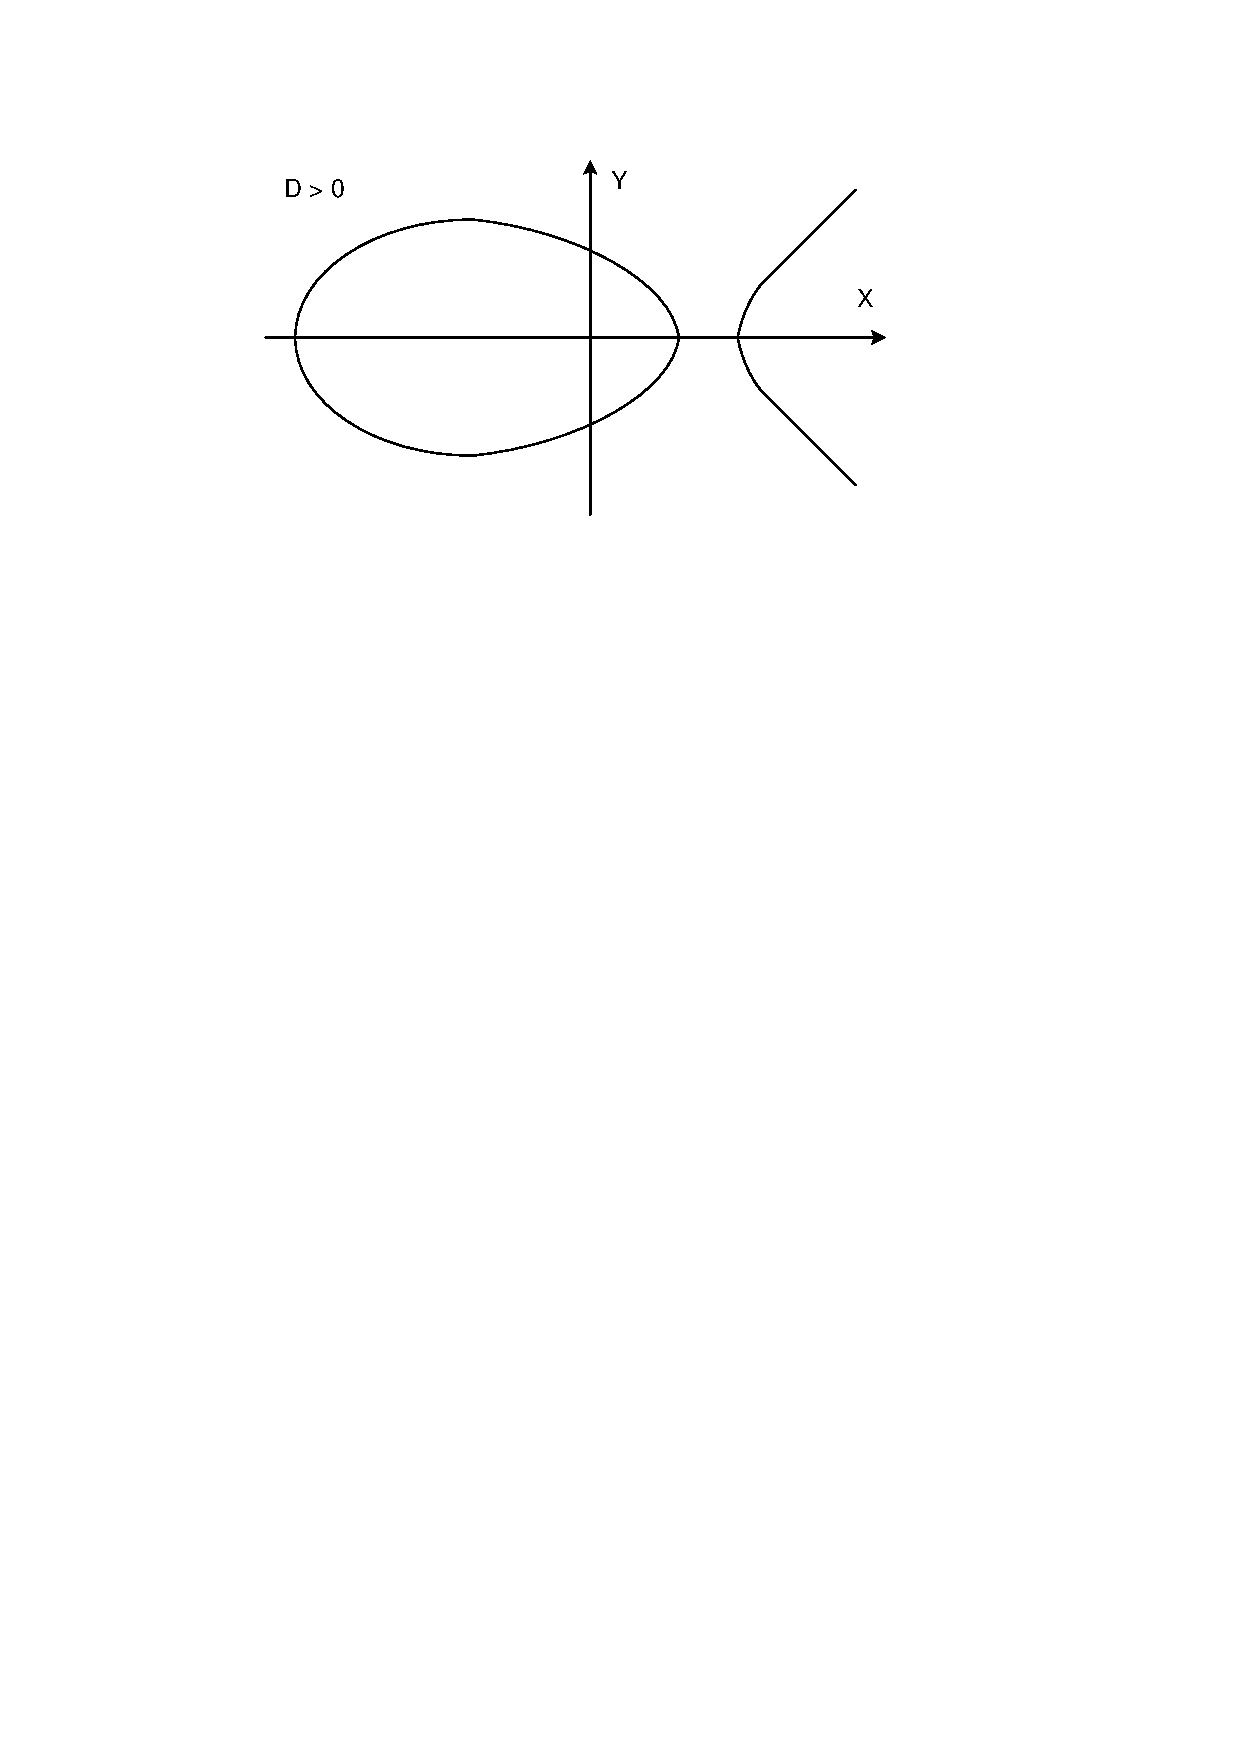
\includegraphics[height=2cm,keepaspectratio]{pic/elliptic-curve-1}}
	~~~~
	\subcaptionbox{$D=0$\label{fig:elliptic-curve-2}}{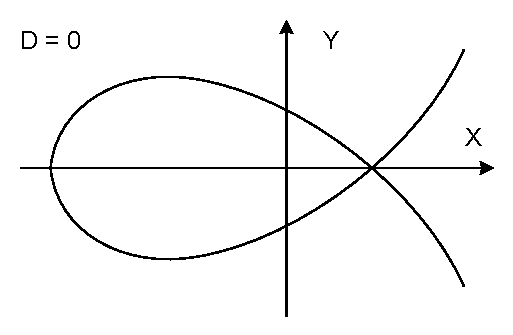
\includegraphics[height=2cm,keepaspectratio]{pic/elliptic-curve-2}}
	~~~~
	\subcaptionbox{$D<0$\label{fig:elliptic-curve-3}}{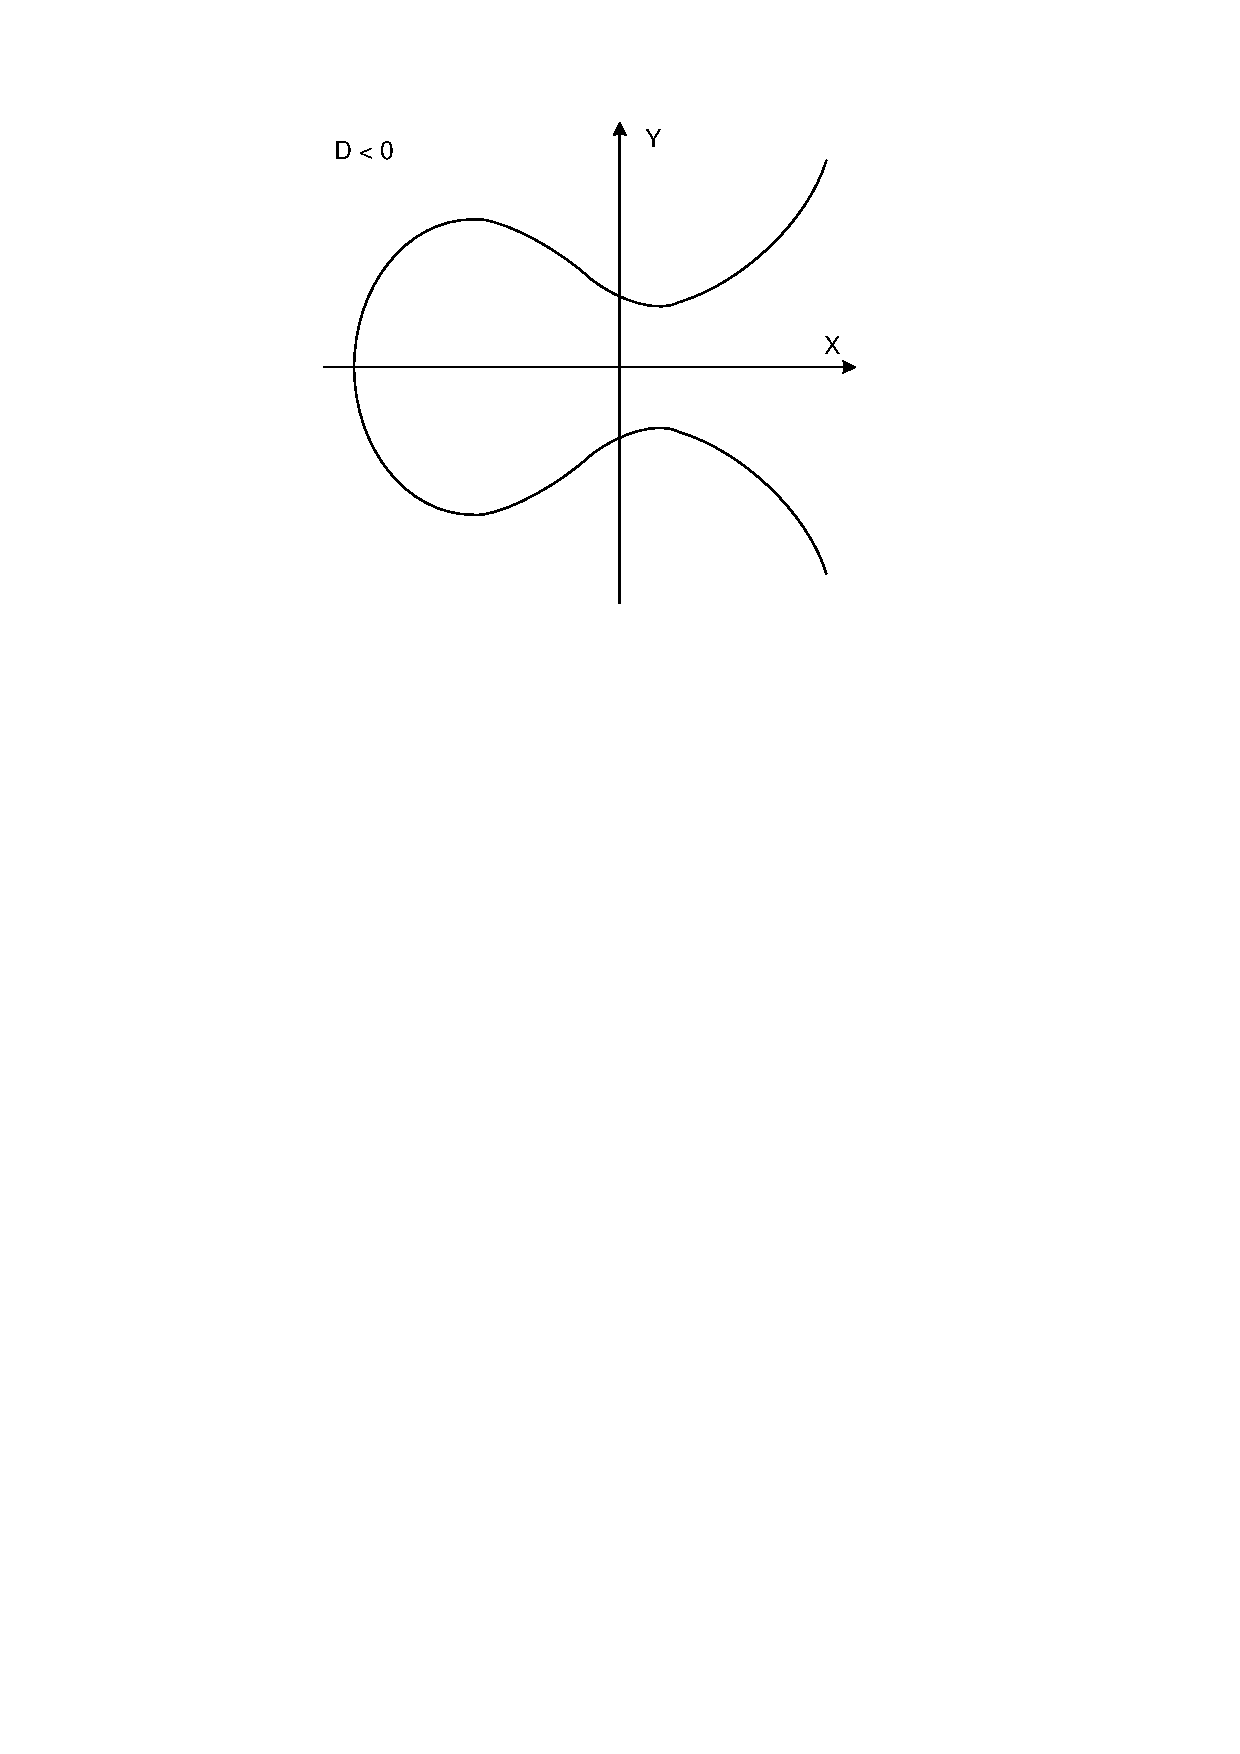
\includegraphics[height=2cm,keepaspectratio]{pic/elliptic-curve-3}}
	\caption{Эллиптические кривые с различными дискриминантами}
\end{figure}

\begin{enumerate}
    \item При $D>0$ график эллиптической кривой состоит из двух частей (см. рис.~\ref{fig:elliptic-curve-1}). Прямая, проходящая через точки $P(x_1; y_1)$ и $Q(x_2; y_2)$, обязательно пересечёт вторую часть кривой в точке с координатами $(x_3; \widetilde{y}_3)$, отображением которой является точка $R(x_3; y_3)$, где $y_3 = - \widetilde{y}_3$. Любые точки на кривой при $D>0$ являются элементами группы по сложению.
    \item Если $D=0$, то левая и правая части касаются в одной точке (см. рис.~\ref{fig:elliptic-curve-2}). Эти кривые называются сингулярными и не рассматриваются.
    \item Если $D<0$, то записанное выше уравнение~\ref{Wer} описывает одну кривую, представленную на рис.~\ref{fig:elliptic-curve-3}.
\end{enumerate}

Рассмотрим операцию сложения точек на эллиптической кривой при $D \ne 0$ (другие кривые не рассматриваются).

Пусть точки $P(x_1; y_1)$ и $Q(x_2; y_2)$ принадлежат эллиптической кривой (рис.~\ref{fig:elliptic-curve-1}). Определим операцию сложения точек
    \[ P + Q = R. \]

\begin{enumerate}
    \item Eсли $P \neq Q$, то точка $R$ определяется как отображение (инвертированная $y$-координата) точки, полученной пересечением эллиптической кривой и прямой $PQ$. Совместно решая уравнения кривой и прямой, можно найти координаты их точки пересечения. Зная координаты точки пересечения, можно вычислить и координаты искомой точки $R = (x_3; y_3)$, которые будут равны:
        \[ x_3 = \lambda^2 - x_1 - x_2, \]
        \[ y_3 = - y_1 + \lambda (x_1 - x_3), \]
где
        \[ \lambda = \frac{y_2 - y_1}{x_2 - x_1} \]
есть тангенс угла наклона между прямой, проходящей через точки $P$ и $Q$, и осью $x$.

	Теперь рассмотрим специальные случаи.
    \item Пусть точки совпадают: $P = Q$. Прямая $PQ$ превращается в касательную к кривой в точке $P$. Находим пересечение касательной с кривой, инвертируем $y$-координату полученной точки, это будет точка $P + P = R$. Тогда $\lambda$ -- тангенс угла между касательной, проведённой к эллиптической кривой в точке $P$, и осью $x$. Запишем уравнение касательной к эллиптической кривой в точке $(x; y)$ в виде:
            \[ 2 y y' = 3 x^2 + a. \]
        Производная равна
            \[ y' = \frac{3 x^2 + a}{2 y}, \]
        и
            \[ \lambda = \frac{3 x_1^2 + a}{2 y_1}. \]
        Координаты $R$ имеют прежний вид:
            \[ x_3 = \lambda^2 - x_1 - x_2, \]
            \[ y_3 = - y_1 + \lambda (x_1 - x_3), \]
    \item Пусть $P$ и $Q$ -- противоположные точки, то есть $P=(x; y)$ и $Q=(x; -y)$. Введём ещё одну точку на бесконечности и обозначим её $O$ (точка $O$ или точка 0 <<ноль>>, или альтернативное обозначение $\infty$). Результатом сложения двух противоположных точек определим точку $O$. Точка $Q$ в данном случае обозначается как $-P$:
        \[ P = (x; y), ~ -P = (x; -y), ~ P + (-P) = O. \]
    \item Пусть $P = (x; 0)$ лежит на оси $x$, тогда
        \[ -P = P, ~ P + P = O. \]
\end{enumerate}

Все точки эллиптической кривой, а также точка $O$ образуют коммутативную группу $\E(\R)$ относительно введённой операции сложения, то есть выполняются законы коммутативной группы\index{группа!точек эллиптической кривой}:
\begin{itemize}
    \item сумма точек $P + Q$ лежит на эллиптической кривой;
    \item существует нулевой элемент -- это точка $O$ на бесконечности:
        \[ \forall P \in \E(\R): ~ O + P = P; \]
    \item для любой точки $P$ существует единственный обратный элемент $-P$:
        \[ P + (-P) = O; \]
    \item выполняется ассоциативный закон:
        \[ (P + Q) + F = P + (Q + F) = P + Q + F; \]
    \item выполняется коммутативный закон:
        \[ P + Q = Q + P. \]
\end{itemize}

Сложение точки с самой собой $d$ раз обозначим как умножение точки на число $d$:
    \[ \underbrace{P + P + \ldots + P}_{d \text{ раз}} = d P. \]


\subsection{Эллиптические кривые над конечным полем}

Эллиптические кривые можно строить не только над полем рациональных чисел, но и над другими полями. То есть координатами точек могут выступать не только числа, принадлежащие полю рациональных чисел $\R$, но и элементы поля комплексных чисел $\mathbb{C}$ или конечного поля $\F$. В криптографии нашли своё применение эллиптические кривые именно над конечными полями.

Далее будем рассматривать эллиптические кривые над конечным полем, являющимся кольцом вычетов по модулю нечётного простого\index{число!простое} числа $p$ (дискриминант не равен 0):
\begin{gather*}
    E: ~ y^2 = x^3 + a x + b, \\
    a, b, x, y \in \Z_p, \\
   \Z_p = \{0, 1, 2, \ldots, p-1\}.
\end{gather*}
Возможна также более компактная запись:
    \[ E: ~ y^2 = x^3 + a x + b \mod p.\]

Точкой эллиптической кривой является пара чисел
    \[ (x; y): x, y \in \Z_p, \]
удовлетворяющая уравнению эллиптической кривой, определённой над конечным полем $\Z_p$.

Операцию сложения двух точек $P = (x_1; y_1)$ и $Q = (x_2; y_2)$ определим точно так же, как и в случае кривой над полем вещественных чисел, описанном выше.

\begin{enumerate}
    \item Две точки $P = (x_1; y_1)$ и $Q = (x_2; y_2)$ эллиптической кривой, определённой над конечным полем $\Z_p$, складываются по правилу:
        \[
            P + Q = R \equiv (x_3; y_3),
        \] \[
            \begin{cases}
                x_3 = \lambda^2 - x_1 - x_2 \mod p,\\
                y_3 = - y_1 + \lambda (x_1 - x_3) \mod p,\\
            \end{cases}
        \]
        где
        \[
            \lambda = \begin{cases}
                \dfrac{y_2 - y_1}{x_2 - x_1} \mod p, & \text{ если } P \ne Q, \\
                \\
                \dfrac{3 x_1^2 + a}{2 y_1} \mod p, & \text{ если } P = Q. \\
            \end{cases}
        \]
    \item Сложение точки $P=(x; y)$ c противоположной \\
        $(-P) = (x; -y)$ даёт точку в бесконечности $O$:
        \begin{gather*}
          P + (-P) = O, \\
         (x_1; y_1) + (x_1; -y_1) = O, \\
         (x_1; 0) + (x_1; 0) = O. 
        \end{gather*}
\end{enumerate}

Мы рассматриваем эллиптические кривые над конечным полем $\Z_p$, где $p > 3$ -- простое\index{число!простое} число, элементы $\Z_p$ -- целые числа $\{0, 1, 2, \ldots, p-1\}$, то есть исследуем следующее уравнение двух переменных $x, y \in \Z_p$:
    \[ y^2 = x^3 + a x + b \mod p, \]
где $a, b \in \Z_p$ -- некоторые константы.

Как и в случае выше, множество точек над конечным полем $\Z_p$, удовлетворяющих уравнению эллиптической кривой, вместе с точкой в бесконечности $O$ образуют конечную группу $\E(\Z_p)$ относительно описанного закона сложения:\index{группа!точек эллиптической кривой}
    \[ \E(\Z_p) ~ \equiv~  O ~ \bigcup ~
        \left\{ (x; y) \in \Z_p \times \Z_p ~\Big|~ y^2 = x^3 + a x + b \mod p \right\}. \]

По теореме Хассе\index{теорема!Хассе} порядок группы точек $|\E(\Z_p)|$ оценивается как
    \[ (\sqrt{p}-1)^2 \leq |\E(\Z_p)| \leq (\sqrt{p}+1)^2, \]
или, в другой записи,
    \[ \Big| |\E(\Z_p)| - p - 1 \Big| \leq 2 \sqrt{p}. \]

\subsection{Примеры группы точек}

\subsubsection{Пример 1}

Пусть эллиптическая кривая задана уравнением
    \[ E: ~ y^2 = x^3 + 1 \mod 7. \]
Найдём все решения этого уравнения, а также количество точек $|\E(\Z_p)|$ на этой эллиптической кривой. Для нахождения решений уравнения составим следующую таблицу:

\begin{center} \begin{tabular}{|c|c|c|c|c|c|c|c|}
    \hline
    $x$ & 0 & 1 & 2 & 3 & 4 & 5 & 6 \\
    \hline
    $y^2$ & 1 & 2 & 2 & 0 & 2 & 0 & 0 \\
    \hline
    $y_1$ & 1 & 3 & 3 & 0 & 3 & 0 & 0 \\
    \hline
    $y_2 = - y_1 \mod p$ & 6 & 4 & 4 &   & 4 &   &   \\
    \hline
\end{tabular} \end{center}

Выпишем все точки, принадлежащие данной эллиптической кривой $\E(\Z_p)$:
\[
    \begin{array}{cccc}
        P_1 = O, & P_2 = (0; 1), & P_3 = (0; 6), & P_4 = (1; 3), \\
        P_5 = (1; 4), & P_6 = (2; 3), & P_7 = (2; 4), & P_8 = (3; 0), \\
        P_9 = (4; 3), & P_{10} = (4; 4), & P_{11} = (5; 0), & P_{12} = (6; 0). \\
    \end{array}
\]

Получили
    \[ |\E(\Z_p)| = 12. \]

Проверим выполнение неравенства Хассе:
    \[ \left| 12 - 7 - 1 \right| = 4 < 2 \sqrt{7}. \]
Следовательно, неравенство Хассе выполняется.

Минимальное натуральное число $s$ такое, что
\[ \underbrace{P + P + \ldots + P}_{s} \equiv s P = O, \]
будем называть \emph{порядком точки $P$}.

%Теорема Лагранжа определяет порядок подгруппы.

\subsubsection{Пример 2}

Группа точек эллиптической кривой
    \[ y^2 = x^3 + 5 x + 6 \mod 17 \]
состоит из точек:
\[ \begin{array}{ccccccc}
    \E(\Z_p) & =~ \Big\{ & (-8; \pm 7), & (-7; \pm 6), & (-6; \pm 7), &   & \\
             &           & (-5; \pm 3), & (-3; \pm 7), & (-1; 0),     & O & \Big\}. \\
\end{array} \]

Порядок группы:
    \[ |\E(\Z_p)| = 12. \]

Порядок группы точек по теореме Хассе:
    \[ (\sqrt{p}-1)^2 \leq |\E(\Z_p)| \leq (\sqrt{p}+1)^2, \]
    \[ 10 \leq 12 \leq 26. \]

Порядки возможных подгрупп: 2, 3, 4, 6 (все возможные делители порядка группы 12).

Найдём порядок точки $A = (-8; 7)$. Так как возможные порядки подгрупп (и всех точек группы) известны, нужно проверить только их.

\begin{itemize}
\item $2A = A + A = (-5; 3)$:
\[\begin{aligned}
& R = P + P, P = (-8; 7), \\
& \lambda = \frac{3 x_P^2 + a}{2y_P} = \frac{3 \cdot (-8)^2 + 5}{2 \cdot 7} = 8 \mod 17, \\
& x_R = \lambda^2 - 2x_P = 8^2 - 2 \cdot (-8) = -5 \mod 17, \\
& y_R = \lambda (x_P - x_R) - y_P = 8 \cdot ((-8) - (-5)) - 7 = 3 \mod 17, \\
& R = (-5; 3). \\
\end{aligned}\]

\item $3A = 2A + A = (-6; 7)$:
\[\begin{aligned}
& R = P + Q, P = (-8; 7), Q = (-5; 3), \\
& \lambda = \frac{y_Q - y_P}{x_Q - x_P} = \frac{3 - 7}{-5 - (-8)} = -7 \mod 17, \\
& x_R = \lambda^2 - x_P - x_Q = (-7)^2 - (-8) - (-5) = -6 \mod 17, \\
& y_R = \lambda (x_P - x_R) - y_P = -7 \cdot (-8 - (-6)) - 7 = 7 \mod 17, \\
& R = (-6; 7). \\
\end{aligned}\]

\item $4A = 2A + 2A = (-5; 3) + (-5; 3) = (-3; 7)$.

\item $6A = 3A + 3A = (-6; 7) + (-6; 7) = (-1; 0)$.

\item $12A = 6A + 6A = (-1; 0) + (-1; 0) = 0$.

\end{itemize}

Найденный порядок точки $A = (-8; 7)$ равен 12, следовательно, она является генератором всей группы.

В таблице~\ref{tab:elliptic-group-sample} найдены порядки точек и циклические подгруппы группы точек $\E(\Z_p)$ такой же эллиптической кривой
    \[ y^2 = x^3 + 5 x + 6 \mod 17. \]
Группа циклическая, число генераторов:
    \[ \varphi(12) = 4. \]
Циклические подгруппы:
    \[ \Gr^{(2)}, ~ \Gr^{(3)}, ~ \Gr^{(4)}, ~ \Gr^{(6)}, \]
верхний индекс обозначает порядок подгруппы.

\begin{table}[!ht]
    \centering
    \caption{Генераторы и циклические подгруппы группы точек эллиптической кривой\label{tab:elliptic-group-sample}}
    \resizebox{\textwidth}{!}{
    \begin{tabular}{|c|l|c|}
        \hline
        Элемент & Порождаемая группа или подгруппа & Порядок \\
        \hline
        $(-8; \pm 7) $ & Вся группа $\E(\Z_p)$ & 12, генератор \\
        $(-7; \pm 6) $ & Вся группа $\E(\Z_p)$ & 12, генератор \\
        $(-6; \pm 7) $ & $\Gr^{(4)} ~=~ \left\{ ~ (-6; \pm 7), ~ (-1; 0), ~ O ~ \right\}$ & 4 \\
        $(-5; \pm 3) $ & $\Gr^{(6)} ~=~ \left\{ ~ (-5; \pm 3), ~ (-3; \pm 7), ~ (-1; 0), ~ O ~ \right\}$ & 6 \\
        $(-3; \pm 7) $ & $\Gr^{(3)} ~=~ \left\{ ~ (-3; \pm 7), ~ O ~ \right\}$ & 3\\
        $(-1; 0)     $ & $\Gr^{(2)} ~=~ \left\{ ~ (-1; 0), ~ O ~ \right\}$ & 2\\
        \hline
    \end{tabular}
    }
\end{table}


\section[Полиномиальные и экспоненциальные алгоритмы]{Полиномиальные и \\ экспоненциальные алгоритмы}

Данный раздел поясняет обоснованность стойкости криптосистем с открытым ключом и имеет лишь косвенное отношение к дискретной математике.

Машина Тьюринга (МТ) (модель, представляющая любой вычислительный алгоритм) состоит из следующих частей:
\begin{itemize}
    \item неограниченная лента, разделённая на клетки; в каждой клетке содержится символ из конечного алфавита, содержащего пустой символ blank; если символ ранее не был записан на ленту, то он считается blank;
    \item печатающая головка, которая может считать, записать символ $a_i$ и передвинуть ленту на 1 клетку влево или вправо $d_k$;
    \item конечная таблица действий
    \[ (q_i, a_j) \rightarrow (q_{i1}, a_{j1}, d_k), \]
где $q$ -- состояние машины.
\end{itemize}

Если таблица переходов однозначна, то машина Тьюринга\index{машина Тьюринга} называется детерминированной. \emph{Детерминированная} машина Тьюринга может \emph{имитировать} любую существующую детерминированную ЭВМ. Если таблица переходов неоднозначна, то есть $(q_i, a_j)$ может переходить по нескольким правилам, то машина \emph{недетерминированная}.

Класс задач $\set{P}$ -- задачи, которые могут быть решены за \emph{полиномиальное} время\index{задача!полиномиальная} на \emph{детерминированной} машине Тьюринга. Пример полиномиальной сложности (количество битовых операций)
    \[ O(k^{\textrm{const}}), \]
где $k$ -- длина входных параметров алгоритма. Операция возведения в степень в модульной арифметике $a^b \mod n$ имеет кубическую сложность $O(k^3)$, где $k$ -- двоичная длина чисел $a,b,n$.

Класс задач $\set{NP}$ -- обобщение класса $\set{P} \subseteq \set{NP}$, включает задачи, которые могут быть решены за \emph{полиномиальное} время на \emph{недетерминированной} машине Тьюринга. Пример сложности задач из $\set{NP}$ -- экспоненциальная сложность\index{задача!экспоненциальная}
    \[ O(\textrm{const}^k). \]
Алгоритм Гельфонда решения задачи дискретного логарифмирования (нахождения $x$ для заданных основания $g$, модуля $p$ и $a = g^x \mod p$), описанный в разделе криптостойкости системы Эль-Гамаля\index{криптосистема!Эль-Гамаля}, имеет сложность $O(e^{k/2})$, где $k$ -- двоичная длина чисел.

В криптографии полиномиальные задачи (относящиеся к классу $\set{P}$) считаются \emph{лёгкими и вычислимыми} на ЭВМ, которые являются детерминированными машинами Тьюринга. Для них, по определению, существуют алгоритмы, работающие за время, полиномиальное относительно размера входных данных. Задачи, относящиеся к классу $\set{NP}$, считаются \emph{трудными и невычислимыми} на ЭВМ, так как все известные на сегодняшний день алгоритмы решения таких задач (в общем случае) требуют экспоненциального времени, а значит всегда можно выбрать такой размер входных данных (читай -- размер ключа шифрования), что время вычисления станет сравнимым с возрастом Вселенной.

Класс $\set{NP}$-полных задач -- подмножество задач из $\set{NP}$, для которых не известен полиномиальный алгоритм для детерминированной машины Тьюринга, и все задачи могут быть сведены друг к другу за полиномиальное время на \emph{детерминированной} машине Тьюринга. Например, задача об укладке рюкзака является $\set{NP}$-полной.

Стойкость криптосистем с \emph{открытым} ключом, как правило, основана на $\set{NP}$ или $\set{NP}$-полных задачах:
\begin{enumerate}
    \item RSA\index{криптосистема!RSA} -- $\set{NP}$-задача факторизации (строго говоря, основана на трудности извлечения корня степени $e$ по модулю $n$).
    \item Криптосистемы типа Эль-Гамаля\index{криптосистема!Эль-Гамаля} -- $\set{NP}$-задача дискретного логарифмирования.
\end{enumerate}

\emph{Нерешённой} проблемой является доказательство неравенства
    \[ \set{P} \neq \set{NP}. \]
Именно на гипотезе о том, что для некоторых задач не существует полиномиальных алгоритмов, и основана стойкость криптосистем с открытым ключом.

\section{Метод индекса совпадений}
\selectlanguage{russian}
\label{chap:coincide-index}

Приведём теоретическое обоснование метода индекса совпадений. Пусть алфавит имеет размер $A$. Пронумеруем его буквы числами от $1$ до $A$. Пусть заданы вероятности появления каждой буквы:
    \[ \mathcal{P} = \left\{ {p_1 ,p_2 , \ldots , p_A } \right\}. \]
В простейшей модели языка предполагается, что тексты состоят из последовательности букв, порождаемых источником независимо друг от друга с известным распределением $\mathcal{P}$.

Найдём индекс совпадений для различных предположений относительно распределений букв последовательности. Сначала рассмотрим случай, когда вероятности всех букв одинаковы. Пусть
    \[ \mathbf{X} = \left[ X_1, X_2, \dots, X_L \right] \]
-- случайный текст с распределением
    \[ \mathcal{P}_1 = \left\{ p_{11}, p_{12}, \dots, p_{1A} \right\}. \]
Найдём индекс совпадений
    \[ I_c(\mathcal{P}_1), \]
то есть вероятность того, что в случайно выбранной паре позиций находятся одинаковые буквы.

Для пары позиций $(k,j)$ найдём условную вероятность $P \left( X_k  = X_j \mid (k,j) \right)$:
    \[ P \left( X_k  = X_j \mid (k,j) \right) ~=~ \sum\limits_{i=1}^A p_{1i}^2 ~\equiv~ k_{p_1}. \]
Эта вероятность не зависит от выбора пары позиций $(k,j)$.

Так как число различных пар равно $\frac{L(L - 1)}{2}$, то вероятность случайного выбора пары $(k,j)$ равна
    \[ P_{(K,J)} (k,j) = \frac{2}{L(L - 1)}. \]
Следовательно,
\begin{multline*}
    I(\mathcal{P}_1) ~= \sum \limits_{1 \leq k < j \leq L} P_{(K,J)}(k,j) ~\cdot~ P(X_k  = X_j \mid (k,j)) =\\
    = \sum \limits_{1 \leq k < j \leq L} \frac{2}{L(L - 1)} k_{p_1} = k_{p_1}.
\end{multline*}

Найдём теперь аналогичную вероятность $I\left( {\mathcal{P}_1 ,\mathcal{P}_2 } \right)$ для случая, когда последовательность независимых случайных букв может быть представлена в виде
\[
\mathbf{X} = \left[ {\begin{array}{*{20}c}
   {X_1 ,}  \\
   {Y_1 ,}  \\
 \end{array} \begin{array}{*{20}c}
   {X_2 ,}  \\
   {Y_2 ,}  \\
 \end{array} \begin{array}{*{20}c}
   { \ldots ,}  \\
   { \ldots ,}  \\
 \end{array} \begin{array}{*{20}c}
   {X_{L/2} }  \\
   {Y_{L/2} }  \\
 \end{array} } \right],
\]
где одинаково распределённые случайные буквы в первой строке имеют распределение:
    \[ \mathcal{P}_1  = \left\{ {p_{11} ,p_{12} , \ldots , p_{1A} } \right\}, \]
а одинаково распределённые случайные буквы во второй строке имеют другое распределение:
    \[ \mathcal{P}_2  = \left\{ {p_{21} ,p_{22} , \ldots , p_{2A} } \right\}. \]

В этом случае сумму по всем парам мы разделяем на три суммы: по парам внутри позиций первой строки, по парам внутри позиций второй строки и по парам, в которых первая позиция берётся из первой строки, а вторая -- из второй:
\begin{multline*}
I(\mathcal{P}_1, \mathcal{P}_2) =
        \frac{2}{L(L - 1)} \cdot \left(
        \sum \limits_{1 \leq k < j \leq L/2} P( X_k  = X_j \mid ( k,j )) + \right.
\\
        \left. + \sum\limits_{1 \leq k < j \leq L/2} P(Y_k  = Y_j \mid (k,j)) +
            \sum\limits_{k=1}^{L/2} \sum\limits_{j=1}^{L/2} {P(X_k = Y_j \mid (k,j))} \right) =
\\
    = \frac{2}{L(L - 1)} \left( \frac{1}{2} \frac{L}{2} \left( \frac{L}{2} - 1 \right) k_{p_1} +
        \frac{1}{2} \frac{L}{2} \left( \frac{L}{2} - 1 \right) k_{p_2} +
        \left( \frac{L}{2} \right)^2 k_{p_1, p_2} \right),
\end{multline*}
где обозначено
    \[ k_{p_1, p_2}  = \sum\limits_{i=1}^A p_{1,i} p_{2,i}. \]

В общем случае рассмотрим последовательность, представленную в виде матрицы, состоящей из $m$ строк и $\frac{L}{m}$ столбцов, где
\[
{\mathbf X} = \left[ {\begin{array}{*{20}c}
   {X_1 } & {X_2 } &  \cdots  & {X_{L/m} }  \\
   {Y_1 } & {Y_2 } &  \cdots  & {Y_{L/m} }  \\
    \vdots  &  \vdots  &  \ddots  &  \vdots   \\
   {Z_1 } & {Z_2 } &  \cdots  & {Z_{L/m} }  \\
\end{array}} \right].
\]

Считаем, что одинаково распределённые случайные буквы в первой строке имеют распределение
    \[ P_1  = \left\{ {p_{11} ,p_{12} , \ldots , p_{1A} } \right\}, \]
одинаково распределённые случайные буквы во второй строке имеют распределение
    \[ P_2  = \left\{ {p_{21} ,p_{22} , \ldots , p_{2A} } \right\} \]
и~т.\,д., одинаково распределённые случайные буквы $m$-й строки имеют распределение
    \[ P_m  = \left\{ {p_{m1},p_{m2} , \ldots , p_{mA} } \right\}. \]

Для вычисления вероятности того, что в случайно выбранной паре позиций будут одинаковые буквы, выполним суммирование по различным парам внутри строк и по парам между различными строками. Аналогично предыдущему случаю получим:
\begin{multline*}
I(\mathcal{P}_1, \mathcal{P}_2, \ldots, \mathcal{P}_m ) = \\
= \frac{2}{L(L - 1)} \left( \frac{L}{2m} \left( \frac{L}{m} - 1 \right) k_{p_1} + \frac{L}{2m} \left( \frac{L}{m} - 1 \right) k_{p_2} + \right. \\
+ \dots + \left. \frac{L}{2m} \left( \frac{L}{m} - 1 \right) k_{p_m} \right) + \\
+ \frac{2}{L(L - 1)} \left( \left( \frac{L}{m} \right)^2 k_{p_1, p_2} + \left( \frac{L}{m} \right)^2 k_{p_1, p_3} + \dots + \left( \frac{L}{m} \right)^2 k_{p_{m - 1}, p_m } \right).
\end{multline*}

Первая сумма содержит $m$ слагаемых, вторая -- $ \frac{m(m-1)}{2}$ слагаемых. Полагая
    \[ k_{p_1} = k_{p_2} = \dots = k_{p_m} = k_p, \]
    \[ k_{p_i p_j } = k_r = \frac{1}{A}, ~ i \ne j, \]
получим после несложных выкладок
    \[ m = \frac{k_p  - k_r}{I - k_r  + \frac{k_p  - I}{L}}. \]


\chapter{Примеры задач}
\selectlanguage{russian}
\taskinit

В данном разделе приведены примеры задач, которые использовались на контрольных работах в МФТИ по курсу <<Защита информации>> в 2011--2015 годах.

\section{Математические основы}
\tasksection

\tasknumber Найдите общее количество генераторов аддитивной циклической группы $\mathbb{Z}_{33}$ с операцией в виде сложения чисел по модулю 33 и перечислите их.
\medbreak
\textbf{Ответ:} 20: [1, 2, 4, 5, 7, 8, 10, 13, 14, 16, 17, 19, 20, 23, 25, 26, 28, 29, 31, 32].
\bigbreak

\tasknumber Вычислить в поле Галуа $GF\left( {2^{5} } \right)$, $m\left( x \right) = x^{5} + x^{3} + x^{2} + x + 1$, следующее значение: $28 \times 29 + 23^2$. Многочлены заданы как десятичное представление двоичных коэффициентов, свободный член многочлена соответствует младшему биту двоичного представления. В ответе привести в десятичном представлении результаты умножения, возведения в степень и сложения.
\medbreak
\textbf{Решение:}
\begin{itemize}\itemsep1pt \parskip0pt \parsep0pt
	\item $a = "28" \Rightarrow a\left( x \right) = x^{4} + x^{3} + x^{2}$;
	\item $b = "29" \Rightarrow b\left( x \right) = x^{4} + x^{3} + x^{2} + 1$;
	\item $c = "23" \Rightarrow c\left( x \right) = x^{4} + x^{2} + x + 1$;
	\item $a \left( x \right) \times b \left( x \right) = x^{4} + x^{3} + x + 1 \Rightarrow a \times b = "27"$;
	\item $c \left( x \right)^2 = x^{4} + x^{3} + x^{2} \Rightarrow c^2 = "28"$;
	\item $result\left( x \right) = x^{2} + x + 1 \Rightarrow result = "7"$.
\end{itemize}
\medbreak
\textbf{Ответ:} <<27>>; <<28>>; <<7>>.
\bigbreak

\tasknumber Вычислить в поле Галуа $GF\left( 27 \right)$, $m\left( x \right) = x^{3} + x^{2} + x + 2$, следующее значение: $26 \times 11 + 25^2$. Многочлены заданы как десятичное представление троичных коэффициентов, свободный член многочлена соответствует младшему триту троичного представления. В ответе привести в десятичном представлении результаты умножения, возведения в степень и сложения.
\medbreak
\textbf{Решение:}
\begin{itemize}\itemsep1pt \parskip0pt \parsep0pt
	\item $a = "26" \Rightarrow a\left( x \right) = 2 x^{2} + 2 x + 2$;
	\item $b = "11" \Rightarrow b\left( x \right) = x^{2} + 2$;
	\item $c = "25" \Rightarrow c\left( x \right) = 2 x^{2} + 2 x + 1$;
	\item $a \left( x \right) \times b \left( x \right) = x^{2} + 1 \Rightarrow a \times b = "10"$;
	\item $c ^2\left( x \right) = x + 2 \Rightarrow c^2 = "5"$;
	\item $result\left( x \right) = x^{2} + x \Rightarrow result = "12"$.
\end{itemize}
\medbreak
\textbf{Ответ:} <<10>>; <<5>>; <<12>>.
\bigbreak

\tasknumber Используя алгоритм быстрого возведения в степень (с помощью разложения показателя степени по степеням двойки по схеме <<слева направо>>), вычислить ${175}^{235} \mod {257}$.
\medbreak
\textbf{Решение:}
\begin{itemize}\itemsep1pt \parskip0pt \parsep0pt
	\item двоичная форма записи степени: $235_{10} = 11101011_{2}$;
	\item полное выражение для вычисления: $(((((((1 \times {175}^1)^2 \times {175}^1)^2 \times {175}^1)^2 \times {175}^0)^2 \times {175}^1)^2 \times {175}^0)^2 \times {175}^1)^2 \times {175}^1\mod 257$;
	\item шаг \No1: $1^2 \times 175 \mod 257  = 175$;
	\item шаг \No2: $175^2 \times 175 \mod 257 = 154$;
	\item шаг \No3: $154^2 \times 175 \mod 257 = 7$;
	\item шаг \No4: $7^2 \mod 257 = 49 \mod 257 = 49$;
	\item шаг \No5: $49^2 \times 175 \mod 257 = 237$;
	\item шаг \No6: $237^2 \mod 257 = 143$;
	\item шаг \No7: $143^2 \times 175 \mod 257 = 107$;
	\item шаг \No8: $107^2 \times 175 \mod 257 = 3$.
\end{itemize}
\medbreak
\textbf{Ответ:} 3.
\bigbreak

\section{Общие определения и теория}
\tasksection

\tasknumber Рассмотрим множество паролей, состоящих из 12 строчных и заглавных латинских букв, а также цифр.
\begin{itemize}\itemsep1pt \parskip0pt \parsep0pt
\item Каков размер этого множества?
\item Сколько времени потребуется на взлом шифртекста, зашифрованного данным паролем, если предположить, что во взломе участвуют все компьютеры мира (7~млрд.), а средний компьютер перебирает 300~000 паролей в секунду?\footnote{См. скорости перебора MD5-хэшей\index{хэш-функция!MD5} на странице \texttt{http://openwall.info\hspace{0pt}/wiki\hspace{0pt}/john\hspace{0pt}/benchmarks}.}
\item Каковы затраты электроэнергии в денежном эквиваленте, если средний компьютер потребляет мощность 400~Вт, а стоимость 1~кВт$\times$час составляет 4,68~рубля?
\end{itemize}
\medbreak
\textbf{Решение:}
\begin{itemize}\itemsep1pt \parskip0pt \parsep0pt
	\item общее количество символов: $26 + 26 + 10 = 62$;
	\item общее количество паролей: $62^{12} \approx 3{,}226\times 10^{21}$;
	\item время на перебор: $62^{12} / (3 \times 10^5) / (7 \times 10^9 ) \approx 1{,}54 \times 10^{6}$ сек.;
	\begin{itemize}\itemsep1pt \parskip0pt \parsep0pt
		\item в минутах: $\approx 25605$;
		\item в часах: $\approx 427$;
		\item в днях: $\approx 18$;
	\end{itemize}
	\item стоимость: $427 \times (7 \times 10^9 ) \times 0{,}4 \times 4{,}68 \approx 5{,}59 \times 10^{12}$ руб.
\end{itemize}
\medbreak
\textbf{Ответ:} паролей $3{,}226 \times 10^{21}$; на перебор нужно $1{,}54 \times 10^6$ секунд ($\approx 18$ дней); затраты -- 5,6 триллиона рублей.
\bigbreak

\tasknumber Источник открытого текста характеризуется случайной величиной $X$, принимающей два значения $x_1$ и $x_2$ с вероятностями $p \left( x = x_1 \right) = 1/5$ и $p \left( x = x_2 \right) = 4/5$ соответственно. Источник ключей характеризуется случайной величиной $Z$, независимой от величины $X$, принимающей два значения $z_1$ и $z_2$ с вероятностями $p \left( z = z_1 \right) = 1/6$ и $p \left( z = z_2 \right) = 5/6$ соответственно. Функция шифрования $E_{z} \left( x \right)$ задаётся следующими правилами: $\left( x_1, z_1 \right) \to y_1$, $\left( x_1, z_2 \right) \to y_2$, $\left( x_2, z_1 \right) \to y_2$, $\left( x_2, z_2 \right) \to y_1$.
\begin{enumerate}\itemsep1pt \parskip0pt \parsep0pt
	\item Найдите собственную информацию каждого из сообщений открытого текста в битах.
	\item Найдите энтропию источника сообщений, источника ключей и шифртекста в битах.
	\item Найдите взаимную информацию открытого текста и ключа в битах.
	\item Найдите взаимную информацию открытого текста и шифртекста в битах.
	\item Найдите взаимную информацию ключа и шифртекста в битах.
	\item Найдите апостериорное распределение вероятностей открытого текста для обоих вариантов перехваченных злоумышленником шифртекстов $y_1$ и $y_2$. Используя вычисленные значения, определите, является ли данная шифросистема абсолютно надёжной. Если нет, то что в данной криптосистеме необходимо поменять? Покажите, что апостериорные вероятности после доработки будут удовлетворять необходимым требованиям абсолютно надёжной криптосистемы.
\end{enumerate}
\medbreak
\textbf{Ответ:}
\begin{itemize}\itemsep1pt \parskip0pt \parsep0pt
	\item $I \left( x_1 \right) = \log_2 5 = 2{,}322$ бит; $I \left( x_2 \right) = \log_2 5/4 = 0{,}322$ бит;
	\item $H \left( X \right) = 0{,}722$ бит; $H \left( Z \right) = 0{,}650$ бит; $H \left( Y \right) = 0{,}881$ бит;
	\item $I \left( X ; Z \right) = 0$ бит; $I \left( X; Y \right) = 0{,}231$ бит; $I \left( Y; Z \right) = 0{,}159$ бит;
	\item $p \left( x_1 | y_1 \right) = 1/21$; $p \left( x_2 | y_1 \right) = 20/21$; $p \left( x_1 | y_2 \right) = 5/9$; $p \left( x_2 | y_2 \right) = 4/9$; не является.
\end{itemize}

\section{КСГПСЧ и потоковые шифры}
\tasksection

\tasknumber Привести следующие два элемента последовательности, сформированной линейным конгруэнтным методом, если предыдущие 3 элемента последовательности такие: 348, 65, 139, а все вычисления выполняются в поле $\mathbb{F}_{499}$.
\medbreak
\textbf{Решение:}
\begin{itemize}\itemsep1pt \parskip0pt \parsep0pt
	\item используя предыдущие значения выхода генератора, строим систему уравнений:
		\[\left\{ {\begin{array}{*{20}c}
		348 \cdot a + c = 65 \mod 499 \\
		65 \cdot a + c = 139 \mod 499 \\
		\end{array} } \right. ;\]
	\item из системы уравнений находим $a = 467$ и $c = 223$;
	\item используя найденные значения, находим следующие элементы последовательности:
	\begin{itemize}\itemsep1pt \parskip0pt \parsep0pt
		\item $x_{3} = a x_{2} + c \mod m = 467 \cdot 139 + 223 \mod 499 = 266$;
		\item $x_{4} = a x_{3} + c \mod m = 467 \cdot 266 + 223 \mod 499 = 194$.
	\end{itemize}
\end{itemize}
\medbreak
\textbf{Ответ:} 266, 194.
\bigbreak

\tasknumber Приведите \emph{предыдущие} 5 бит выхода генератора псевдослучайной последовательности, основанного на регистре сдвига с линейной обратной связью, если известно, что характеристический полином регистра -- $m\left(x\right)=x^{5} + x^{3} + 1$ (см. рис.), а дальнейшая последовательность такова: $1, 1, 0, 1, 0, 1$.
\begin{center}
	\begin{tikzpicture}[scale=0.05]
		\draw[black,very thick] (30,30) -- (30,40) -- (40,40) -- (40,30) -- (30,30) -- (30,40);
		\draw[black,thick] (35,40) -- (35,50) -- (35,50) -- (37.5,50);
		\draw[black,very thick] (40,30) -- (40,40) -- (50,40) -- (50,30) -- (40,30) -- (40,40);
		\draw[black,very thick] (50,30) -- (50,40) -- (60,40) -- (60,30) -- (50,30) -- (50,40);
		\draw[black,thick] (55,40) -- (55,47.5);
		\draw[black,thick] (53.5,46) -- (55,47.5) -- (56.5,46);
		\draw[black,thick] (37.5,50) -- (52.5,50);
		\draw[black,thick] (51,51.5) -- (52.5,50) -- (51,48.5);
		\draw (55,50) circle [radius=2.5];
		\draw[black] (52.5,50) -- (57.5,50);
		\draw[black] (55,47.5) -- (55,52.5);
		\draw[black,very thick] (60,30) -- (60,40) -- (70,40) -- (70,30) -- (60,30) -- (60,40);
		\draw[black,very thick] (70,30) -- (70,40) -- (80,40) -- (80,30) -- (70,30) -- (70,40);
		\draw[black,thick] (57.5,50) -- (85,50) -- (85,35) -- (80,35);
		\draw[black,thick] (82.5,36.5) -- (80,35) -- (82.5,33.5);
		\draw[black,thick] (30,35) -- (15,35);
		\draw[black,thick] (20,30) -- (15,35) -- (20,40);
	\end{tikzpicture}
\end{center}
\medbreak
\textbf{Решение.}
\begin{itemize}\itemsep1pt \parskip0pt \parsep0pt
	\item Из коэффициентов многочлена $m\left(x\right)$ получаем формулу предыдущего элемента:
		\[ m\left(x\right) = \sum\limits_{i = 5 \dots 1} {a_i x^i } + 1 = x^{5} + x^{3} + 1; \]
		\[ b_0 = a_5 b_5 \oplus \dots \oplus a_1 b_1 = b_{5} \oplus b_{3}.\]
		Это формула бита, который на следующей итерации станет битом $b_1$, то есть значение функции обратной связи регистра;
	\item $b_5 = b_0\oplus b_{3}$ -- формула выходного бита, если известны остальные биты и значение функции обратной связи;
	\item За счёт последних 5 бит выхода восстанавливаем состояние регистра $\overrightarrow{s_{1}}=\left(b_{1}, b_{2}, b_{3}, b_{4}, b_{5}\right) = \left(1, 0, 1, 0, 1\right)$. Далее начинаем отматывать время назад.
	\item $\overrightarrow{s_{1}}=\left(1, 0, 1, 0, 1\right)$. $\overrightarrow {s_{0}} = \left(0, 1, 0, 1, ? \right)$ и $b_0 = 1$. \\
		$b_5 = b_0\oplus b_{3}=1 \oplus 0=1$. $\overrightarrow{s_{0}}=\left(0, 1, 0, 1, 1\right)$. \\
		Выход — 1;
	\item $\overrightarrow{s_{0}}=\left(0, 1, 0, 1, 1\right)$. $\overrightarrow {s_{-1}} = \left(1, 0, 1, 1, ? \right)$ и $b_0 = 0$. \\
		$b_5 = b_0\oplus b_{3}=0 \oplus 1=1$. $\overrightarrow{s_{-1}}=\left(1, 0, 1, 1, 1\right)$. \\
		Выход — 1;
	\item $\overrightarrow{s_{-1}}=\left(1, 0, 1, 1, 1\right)$. $\overrightarrow {s_{-2}} = \left(0, 1, 1, 1, ? \right)$ и $b_0 = 1$. \\
		$b_5 = b_0\oplus b_{3}=1 \oplus 1=0$. $\overrightarrow{s_{-2}}=\left(0, 1, 1, 1, 0\right)$. \\
		Выход — 0;
	\item $\overrightarrow{s_{-2}}=\left(0, 1, 1, 1, 0\right)$. $\overrightarrow {s_{-3}} = \left(0, 0, 1, 1, ? \right)$ и $b_0 = 0$. \\
		$b_5 = b_0\oplus b_{3}=0 \oplus 1=1$. $\overrightarrow{s_{-3}}=\left(1, 1, 1, 0, 1\right)$. \\
		Выход — 1;
	\item $\overrightarrow{s_{-3}}=\left(1, 1, 1, 0, 1\right)$. $\overrightarrow {s_{-4}} = \left(0, 1, 0, 1, ? \right)$ и $b_0 = 1$. \\
		$b_5 = b_0\oplus b_{3}=1 \oplus 0=1$. $\overrightarrow{s_{-4}}=\left(1, 1, 0, 1, 1\right)$. \\
		Выход — 1;
	\item $\overrightarrow{s_{-4}}=\left(1, 1, 0, 1, 1\right)$. $\overrightarrow {s_{-5}} = \left(0, 1, 1, 0, ? \right)$ и $b_0 = 1$. \\
		$b_5 = b_0\oplus b_{3}=1 \oplus 1=0$. $\overrightarrow{s_{-5}}=\left(1, 0, 1, 1, 0\right)$. \\
		Выход — 0;
	\item Ответ (в порядке выдачи бит генератором): $0, 1, 1, 0, 1$.
	\item Краткое оформление второй части задачи можно увидеть в таблице~\ref{table:task-lfsr-1-short-solution}. Таблица заполняется снизу вверх (так как нам нужны предыдущие биты, а не следующие). Последняя строка таблицы соответствует последнему известному состоянию регистра -- последним 5 битам последовательности. Столбцы таблицы связаны формулой $b_{5} \oplus b_{3} = b_0 $. Ответ находится в первых 5 элементах первого столбца.
	\begin{table}[!thb]
		\centering
		\begin{tabular}{ l | c || c c c c c|| c }
		 & & $b_{5}$& $b_{4}$& $b_{3}$& $b_{2}$& $b_{1}$ & $b_0$ \\
		  \hline
		  $\overrightarrow {s_{-5}}$ & 0 & 0 & 1 & 1 & 0 & 1& 1 \\
		  $\overrightarrow {s_{-4}}$ & 1 & 1 & 1 & 0 & 1 & 1& 1 \\
		  $\overrightarrow {s_{-3}}$ & 1 & 1 & 0 & 1 & 1 & 1& 0 \\
		  $\overrightarrow {s_{-2}}$ & 0 & 0 & 1 & 1 & 1 & 0& 1 \\
		  $\overrightarrow {s_{-1}}$ & 1 & 1 & 1 & 1 & 0 & 1& 0 \\
		  $\overrightarrow {s_{0}}$ & 1 & 1 & 1 & 0 & 1 & 0& 1 \\
		  $\overrightarrow {s_{1}}$ & 1 & 1 & 0 & 1 & 0 & 1& $\cdot$ \\
		\hline
		\end{tabular}
		\caption{Краткое оформление решения задачи \No\arabic{task-section}.\arabic{task-number} в виде таблицы}
		\label{table:task-lfsr-1-short-solution}
	\end{table}
\end{itemize}
\medbreak
\textbf{Ответ:} $0, 1, 1, 0, 1$.
\bigbreak

\tasknumber Укажите характеристический полином и приведите следующие 5 бит выхода генератора псевдослучайной последовательности, основанного на регистре сдвига с линейной обратной связью, если известно, что степень характеристического полинома регистра -- $m\left(x\right)$ -- равна 5, а предыдущая последовательность такова: $0, 1, 0, 0, 1, 1, 0, 0, 0, 0, 1$. Порядок бит в последовательности соответствует порядку их генерации РСЛОС.
\medbreak
\textbf{Решение.}
\begin{itemize}\itemsep1pt \parskip0pt \parsep0pt
	\item Каждый бит выходной последовательности есть функция 5 предыдущих выходных бит вида $b_0 = f\left( b_{5} \dots b_1 \right) $. В данных обозначениях $b_{5}$ является наиболее ранним битом, а $b_1$ -- последним, который сгенерировал РСЛОС непосредственно перед генерацией бита $b_0$.  Вид функции задаётся характеристическим многочленом, который и нужно найти.
	\[\begin{array}{l}
		m \left( x \right) = x^{5} +  a_{4} x^{4} + a_{3} x^{3} + a_{2} x^{2} + a_{1} x^{1} +1; \\
		b_{5} \oplus a_{4} b_{4} \oplus a_{3} b_{3} \oplus a_{2} b_{2} \oplus a_{1} b_{1} = b_0. \\
	\end{array}\]
	\[\begin{array}{l}
		f\left(0,1,0,0,1\right) = 1, \\
		f\left(1,0,0,1,1\right) = 0, \\
		f\left(0,0,1,1,0\right) = 0, \\
		f\left(0,1,1,0,0\right) = 0, \\
		f\left(1,1,0,0,0\right) = 0, \\
		f\left(1,0,0,0,0\right) = 1. \\
	\end{array}\]
	\item Это приводит к системе уравнений:
	\[\left\{ {\begin{array}{*{20}c}
		f\left(0,1,0,0,1\right) = 0 \oplus \left( a_{4} \cdot 1\right) \oplus \left( a_{3} \cdot 0\right) \oplus \left( a_{2} \cdot 0\right) \oplus \left( a_{1} \cdot 1\right) = 1 \\
		f\left(1,0,0,1,1\right) = 1 \oplus \left( a_{4} \cdot 0\right) \oplus \left( a_{3} \cdot 0\right) \oplus \left( a_{2} \cdot 1\right) \oplus \left( a_{1} \cdot 1\right) = 0 \\
		f\left(0,0,1,1,0\right) = 0 \oplus \left( a_{4} \cdot 0\right) \oplus \left( a_{3} \cdot 1\right) \oplus \left( a_{2} \cdot 1\right) \oplus \left( a_{1} \cdot 0\right) = 0 \\
		f\left(0,1,1,0,0\right) = 0 \oplus \left( a_{4} \cdot 1\right) \oplus \left( a_{3} \cdot 1\right) \oplus \left( a_{2} \cdot 0\right) \oplus \left( a_{1} \cdot 0\right) = 0 \\
		f\left(1,1,0,0,0\right) = 1 \oplus \left( a_{4} \cdot 1\right) \oplus \left( a_{3} \cdot 0\right) \oplus \left( a_{2} \cdot 0\right) \oplus \left( a_{1} \cdot 0\right) = 0 \\
		f\left(1,0,0,0,0\right) = 1 \oplus \left( a_{4} \cdot 0\right) \oplus \left( a_{3} \cdot 0\right) \oplus \left( a_{2} \cdot 0\right) \oplus \left( a_{1} \cdot 0\right) = 1 \\
	\end{array} } \right.\]
	\[\left\{ {\begin{array}{*{20}l}
		a_{4} \oplus a_{1} = 1 \\
		a_{2} \oplus a_{1} = 1 \\
		a_{3} \oplus a_{2} = 0 \\
		a_{4} \oplus a_{3} = 0 \\
		a_{4} = 1 \\
	\end{array} } \right.\]
	\item Найденные из системы уравнения коэффициенты $\left(a_{4}, a_{3}, a_{2}, a_{1}\right) = \left(1 , 1 , 1 , 0\right)$.
	\item Характеристический полином регистра:
		\[\begin{array}{l}
			m \left( x \right) = x^{5}+ a_{4} x^{4}+ a_{3} x^{3}+ a_{2} x^{2}+ a_{1} x^{1} + 1; \\
			m = x^{5} + x^{4} + x^{3} + x^{2} + 1. \\
		\end{array}\]
	\item Схема РСЛОС приведена на рисунке.
	\begin{center}
		\begin{tikzpicture}[scale=0.05]
			\draw[black,very thick] (30,30) -- (30,40) -- (40,40) -- (40,30) -- (30,30) -- (30,40);
			\draw[black,thick] (35,40) -- (35,50) -- (35,50) -- (37.5,50);
			\draw[black,very thick] (40,30) -- (40,40) -- (50,40) -- (50,30) -- (40,30) -- (40,40);
			\draw[black,thick] (45,40) -- (45,47.5);
			\draw[black,thick] (43.5,46) -- (45,47.5) -- (46.5,46);
			\draw[black,thick] (37.5,50) -- (42.5,50);
			\draw[black,thick] (41,51.5) -- (42.5,50) -- (41,48.5);
			\draw (45,50) circle [radius=2.5];
			\draw[black] (42.5,50) -- (47.5,50);
			\draw[black] (45,47.5) -- (45,52.5);
			\draw[black,very thick] (50,30) -- (50,40) -- (60,40) -- (60,30) -- (50,30) -- (50,40);
			\draw[black,thick] (55,40) -- (55,47.5);
			\draw[black,thick] (53.5,46) -- (55,47.5) -- (56.5,46);
			\draw[black,thick] (47.5,50) -- (52.5,50);
			\draw[black,thick] (51,51.5) -- (52.5,50) -- (51,48.5);
			\draw (55,50) circle [radius=2.5];
			\draw[black] (52.5,50) -- (57.5,50);
			\draw[black] (55,47.5) -- (55,52.5);
			\draw[black,very thick] (60,30) -- (60,40) -- (70,40) -- (70,30) -- (60,30) -- (60,40);
			\draw[black,thick] (65,40) -- (65,47.5);
			\draw[black,thick] (63.5,46) -- (65,47.5) -- (66.5,46);
			\draw[black,thick] (57.5,50) -- (62.5,50);
			\draw[black,thick] (61,51.5) -- (62.5,50) -- (61,48.5);
			\draw (65,50) circle [radius=2.5];
			\draw[black] (62.5,50) -- (67.5,50);
			\draw[black] (65,47.5) -- (65,52.5);
			\draw[black,very thick] (70,30) -- (70,40) -- (80,40) -- (80,30) -- (70,30) -- (70,40);
			\draw[black,thick] (67.5,50) -- (85,50) -- (85,35) -- (80,35);
			\draw[black,thick] (82.5,36.5) -- (80,35) -- (82.5,33.5);
			\draw[black,thick] (30,35) -- (15,35);
			\draw[black,thick] (20,30) -- (15,35) -- (20,40);
		\end{tikzpicture}
	\end{center}
	\item Теперь, когда характеристический полином известен, восстанавливаем состояния регистра по последним 5 выходным битам:
	\begin{itemize}\itemsep1pt \parskip0pt \parsep0pt
		\item $\left(b_{5}, b_{4}, b_{3}, b_{2}, b_{1}\right) = \left(0, 0, 0, 0, 1\right)$. Сумма: $b_0 = b_{5} \oplus b_{4} \oplus b_{3} \oplus b_{2}=0 \oplus 0 \oplus 0 \oplus 0=0$. Следующее состояние $\left(0, 0, 0, 1, 0\right)$, а текущий выход $b_{5}=0$.
		\item $\left(b_{5}, b_{4}, b_{3}, b_{2}, b_{1}\right) = \left(0, 0, 0, 1, 0\right)$. Сумма: $b_0 = b_{5} \oplus b_{4} \oplus b_{3} \oplus b_{2}=0 \oplus 0 \oplus 0 \oplus 1=1$. Следующее состояние $\left(0, 0, 1, 0, 1\right)$, а текущий выход $b_{5}=0$.
		\item $\left(b_{5}, b_{4}, b_{3}, b_{2}, b_{1}\right) = \left(0, 0, 1, 0, 1\right)$. Сумма: $b_0 = b_{5} \oplus b_{4} \oplus b_{3} \oplus b_{2}=0 \oplus 0 \oplus 1 \oplus 0=1$. Следующее состояние $\left(0, 1, 0, 1, 1\right)$, а текущий выход $b_{5}=0$.
		\item $\left(b_{5}, b_{4}, b_{3}, b_{2}, b_{1}\right) = \left(0, 1, 0, 1, 1\right)$. Сумма: $b_0 = b_{5} \oplus b_{4} \oplus b_{3} \oplus b_{2}=0 \oplus 1 \oplus 0 \oplus 1=0$. Следующее состояние $\left(1, 0, 1, 1, 0\right)$, а текущий выход $b_{5}=0$.
		\item $\left(b_{5}, b_{4}, b_{3}, b_{2}, b_{1}\right) = \left(1, 0, 1, 1, 0\right)$. Сумма: $b_0 = b_{5} \oplus b_{4} \oplus b_{3} \oplus b_{2}=1 \oplus 0 \oplus 1 \oplus 1=1$. Следующее состояние $\left(0, 1, 1, 0, 1\right)$, а текущий выход $b_{5}=1$.
	\end{itemize}
	\item Следующие итерации, дающие нужный ответ:
	\begin{itemize}\itemsep1pt \parskip0pt \parsep0pt
		\item $\left(b_{5}, b_{4}, b_{3}, b_{2}, b_{1}\right) = \left(0, 1, 1, 0, 1\right)$. Сумма: $b_0 = b_{5} \oplus b_{4} \oplus b_{3} \oplus b_{2}=0 \oplus 1 \oplus 1 \oplus 0=0$. Следующее состояние $\left(1, 1, 0, 1, 0\right)$, а текущий выход $b_{5}=0$.
		\item $\left(b_{5}, b_{4}, b_{3}, b_{2}, b_{1}\right) = \left(1, 1, 0, 1, 0\right)$. Сумма: $b_0 = b_{5} \oplus b_{4} \oplus b_{3} \oplus b_{2}=1 \oplus 1 \oplus 0 \oplus 1=1$. Следующее состояние $\left(1, 0, 1, 0, 1\right)$, а текущий выход $b_{5}=1$.
		\item $\left(b_{5}, b_{4}, b_{3}, b_{2}, b_{1}\right) = \left(1, 0, 1, 0, 1\right)$. Сумма: $b_0 = b_{5} \oplus b_{4} \oplus b_{3} \oplus b_{2}=1 \oplus 0 \oplus 1 \oplus 0=0$. Следующее состояние $\left(0, 1, 0, 1, 0\right)$, а текущий выход $b_{5}=1$.
		\item $\left(b_{5}, b_{4}, b_{3}, b_{2}, b_{1}\right) = \left(0, 1, 0, 1, 0\right)$. Сумма: $b_0 = b_{5} \oplus b_{4} \oplus b_{3} \oplus b_{2}=0 \oplus 1 \oplus 0 \oplus 1=0$. Следующее состояние $\left(1, 0, 1, 0, 0\right)$, а текущий выход $b_{5}=0$.
		\item $\left(b_{5}, b_{4}, b_{3}, b_{2}, b_{1}\right) = \left(1, 0, 1, 0, 0\right)$. Сумма: $b_0 = b_{5} \oplus b_{4} \oplus b_{3} \oplus b_{2}=1 \oplus 0 \oplus 1 \oplus 0=0$. Следующее состояние $\left(0, 1, 0, 0, 0\right)$, а текущий выход $b_{5}=1$.
		\end{itemize}
	\item Итого ответ на вторую часть задачи: $0, 1, 1, 0, 1$.
	\item Краткое оформление второй части задачи можно увидеть в таблице~\ref{table:task-lfsr-2-short-solution}. Таблица заполняется сверху вниз. Столбцы таблицы связаны формулой $b_{5} \oplus b_{4} \oplus b_{3} \oplus b_{2} = b_0 $. В первой строке записаны первые 5 бит полученной последовательности. Выполняя последовательно операции над регистром, мы получим все следующие биты. Начать заполнение таблицы можно со строчки $\overrightarrow s_{6}$ (то есть с последних 5 бит, данных в условии задачи), строки выше приведены для возможности (само)контроля студента. Ответом являются последние 5 бит в первом столбце.
	\begin{table}[!thb]
		\centering
		\begin{tabular}{ l | c || c c c c c|| c }
		 & & $b_{5}$& $b_{4}$& $b_{3}$& $b_{2}$& $b_{1}$ & $b_0$ \\
		  \hline
		  $\overrightarrow {s_{0}}$ & 0 & 0 & 1 & 0 & 0 & 1& 1 \\
		  \hline
		  $\overrightarrow {s_{1}}$ & 1 & 1 & 0 & 0 & 1 & 1& 0 \\
		  $\overrightarrow {s_{2}}$ & 0 & 0 & 0 & 1 & 1 & 0& 0 \\
		  $\overrightarrow {s_{3}}$ & 0 & 0 & 1 & 1 & 0 & 0& 0 \\
		  $\overrightarrow {s_{4}}$ & 1 & 1 & 1 & 0 & 0 & 0& 0 \\
		  $\overrightarrow {s_{5}}$ & 1 & 1 & 0 & 0 & 0 & 0& 1 \\
		  \hline
		  $\overrightarrow {s_{6}}$ & 0 & 0 & 0 & 0 & 0 & 1& 0 \\
		  $\overrightarrow {s_{7}}$ & 0 & 0 & 0 & 0 & 1 & 0& 1 \\
		  $\overrightarrow {s_{8}}$ & 0 & 0 & 0 & 1 & 0 & 1& 1 \\
		  $\overrightarrow {s_{9}}$ & 0 & 0 & 1 & 0 & 1 & 1& 0 \\
		  $\overrightarrow {s_{10}}$ & 1 & 1 & 0 & 1 & 1 & 0& 1 \\
		  \hline
		  $\overrightarrow {s_{11}}$ & 0 & 0 & 1 & 1 & 0 & 1& 0 \\
		  $\overrightarrow {s_{12}}$ & 1 & 1 & 1 & 0 & 1 & 0& 1 \\
		  $\overrightarrow {s_{13}}$ & 1 & 1 & 0 & 1 & 0 & 1& 0 \\
		  $\overrightarrow {s_{14}}$ & 0 & 0 & 1 & 0 & 1 & 0& 0 \\
		  $\overrightarrow {s_{15}}$ & 1 & 1 & 0 & 1 & 0 & 0& 0 \\
		\hline
		\end{tabular}
		\caption{Краткое оформление решения второй части задачи \No\arabic{task-section}.\arabic{task-number} в виде таблицы}
		\label{table:task-lfsr-2-short-solution}
	\end{table}
\end{itemize}
\medbreak
\textbf{Ответ:} полином $m \left( x \right) = x^{5} + x^{4} + x^{3} + x^{2} + 1$; дальнейшая последовательность: $0, 1, 1, 0, 1$.

\section{Псевдопростые числа}
\tasksection

\tasknumber Проверить, являются ли числа 73, 95 свидетелями простоты числа 111 по Ферма.
\medbreak
\textbf{Ответ:} да; нет.
\bigbreak

\tasknumber Проверить, являются ли числа 74, 448, 640, 660, 719 свидетелями простоты числа 793 по Миллеру.
\medbreak
\textbf{Ответ:} да; да; нет; нет; да.
\bigbreak

\section{Криптосистема RSA}
\tasksection

\tasknumber Зашифровать сообщение по схеме RSA. Открытый ключ: $n = 323$; $e = 245$. Сообщение: $m = 307$.
\medbreak
\textbf{Ответ:} $c = 86$.
\bigbreak

\tasknumber Расшифровать сообщение по схеме RSA. Для генерации пары открытого и закрытого ключа использовались числа: $p = 13$; $q = 17$. Открытая экспонента: $e = 91$. Зашифрованное сообщение: $c = 196$.
\medbreak
\textbf{Ответ:} $d = 19$; $m = 66$.
\bigbreak

\tasknumber Расшифровать сообщение по схеме RSA. Открытый ключ: $n = 85$; $e = 15$. Зашифрованное сообщение: $c = 32$.
\medbreak
\textbf{Ответ:} $p = 5$; $q = 17$; $d = 47$; $m = 8$.
\bigbreak

\tasknumber Подписать сообщение по схеме RSA. Закрытый ключ: $n = 437$; $d = 181$. Сообщение: $m = 84$.
\medbreak
\textbf{Ответ:} $s = 122$.
\bigbreak

\tasknumber Подписать сообщение по схеме RSA. Открытый ключ: $n = 253$; $e = 159$. Сообщение: $m = 193$.
\medbreak
\textbf{Ответ:} $n = 11 \cdot 23$; $d = 119$; $s = 2$.

\section{Криптосистема Эль-Гамаля}
\tasksection

\tasknumber Зашифровать сообщение по схеме Эль-Гамаля. Открытый ключ: $p = 29$; $g = 10$; $y = 8$. Закрытый ключ: $x = 5$. Сообщение: $M = 4$. Использовать следующий случайный параметр для шифрования: $k = 5$.
\medbreak
\textbf{Ответ:} $c = (a; b) = (8; 21)$.
\bigbreak

\tasknumber Расшифровать сообщение по схеме Эль-Гамаля. Открытый ключ: $p = 23$; $g = 5$; $y = 9$. Закрытый ключ: $x = 10$. Зашифрованное сообщение: $\left( 10, 18\right)$.
\medbreak
\textbf{Ответ:} $m = 4$.
\bigbreak

\tasknumber Расшифровать сообщение по схеме Эль-Гамаля. Открытый ключ: $p = 29$; $g = 15$; $y = 28$. Закрытый ключ: $x = 14$. Зашифрованное сообщение: $\left( 10, 23\right)$.
\medbreak
\textbf{Ответ:} $m = 6$.
\bigbreak

\tasknumber Проверить подпись по схеме Эль-Гамаля. Открытый ключ: $p = 29$; $g = 14$; $y = 7$. Сообщение: $m = 7$. Подпись: $a = 19$;  $b = 19$.
\medbreak
\textbf{Ответ:} $S = 12$.
\bigbreak

\tasknumber Подписать сообщение по схеме Эль-Гамаля. Открытый ключ: $p = 23$; $g = 20$; $y = 17$. Сообщение: $m = 4$. Использовать следующий случайный параметр для создания подписи: $k = 7$.
\medbreak
\textbf{Ответ:} $x = 19$; $s = (a; b) = (21; 19)$.
\bigbreak

\section{Эллиптические кривые}
\tasksection

\tasknumber Для точки A (8; 6), принадлежащей группе точек эллиптической кривой $y^2 = x^3 - 9x - 13$ над конечным полем $\mathbb{F}_{17}$, найти координаты точек $B = 2 \times A = A + A$ и $C = 3 \times A = A + A + A$.
\medbreak
\textbf{Ответ:} $(3; 15)$, $(14; 15)$.
\bigbreak

\tasknumber Найти группу точек (перечислить все точки) эллиптической кривой $y^2 = x^3 - 2 x - 10$ над конечным полем $\mathbb{F}_{13}$.
\medbreak
\textbf{Решение:} получение группы точек с помощью таблицы:\\
\begin{tabular}{|r|r|r|r|r|r|r|r|}
\hline
$x$ & $x^2$ & $x^3$ & $-2x$ & $-10$ & $y^2$ & $y_1$, $y_2$ & точки \\ 
\hline
$0$ & $0$ & $0$ & $-0$ & $-10$ & $3$ & $4$,$9$ &$(0; 4)$, $(0; 9)$ \\ 
$1$ & $1$ & $1$ & $-2$ & $-10$ & $2$ &  --- & --- \\ 
$2$ & $4$ & $8$ & $-4$ & $-10$ & $7$ &  --- & --- \\ 
$3$ & $9$ & $1$ & $-6$ & $-10$ & $11$ &  --- & --- \\ 
$4$ & $3$ & $12$ & $-8$ & $-10$ & $7$ &  --- & --- \\ 
$5$ & $12$ & $8$ & $-10$ & $-10$ & $1$ & $1$,$12$ &$(5; 1)$, $(5; 12)$ \\ 
$6$ & $10$ & $8$ & $-12$ & $-10$ & $12$ & $5$,$8$ &$(6; 5)$, $(6; 8)$ \\ 
$7$ & $10$ & $5$ & $-1$ & $-10$ & $7$ &  --- & --- \\ 
$8$ & $12$ & $5$ & $-3$ & $-10$ & $5$ &  --- & --- \\ 
$9$ & $3$ & $1$ & $-5$ & $-10$ & $12$ & $5$,$8$ &$(9; 5)$, $(9; 8)$ \\ 
$10$ & $9$ & $12$ & $-7$ & $-10$ & $8$ &  --- & --- \\ 
$11$ & $4$ & $5$ & $-9$ & $-10$ & $12$ & $5$,$8$ &$(11; 5)$, $(11; 8)$ \\ 
$12$ & $1$ & $12$ & $-11$ & $-10$ & $4$ & $2$,$11$ &$(12; 2)$, $(12; 11)$ \\ 
\hline
\end{tabular}
\medbreak
\textbf{Ответ:}
\begin{itemize}
\item Точки эллиптической кривой: $[(0; 4)$, $(0; 9)$, $(5; 1)$, $(5; 12)$, $(6; 5)$, $(6; 8)$, $(9; 5)$, $(9; 8)$, $(11; 5)$, $(11; 8)$, $(12; 2)$, $(12; 11)$, $O]$;
\item Размер группы точек: $13$.
\end{itemize}
\bigbreak

\tasknumber Для точки $\left(6; 9\right)$ определить, является ли она генератором всей группы точек кривой $y^2 = x^3 - 10 x - 7$ над конечным полем $\mathbb{F}_{17}$ или подгруппы. Перечислить точки генерируемой подгруппы (группы).
\medbreak
\textbf{Ответ:} точка $\left(6; 9\right)$ — генератор подгруппы размера 4: $[(6; 9), (4; 0), (6; 8), O]$.
\bigbreak

\tasknumber Вычислить электронную подпись сообщения $m=5$ по схеме ГОСТ Р 34.10-2012. Кривая $y^2 = x^3 - 3 x - 8$ над конечным полем $\mathbb{F}_{11}$. В качестве генератора используется точка G$\left(0; 5\right)$, размер циклической подгруппы -- $16$. Открытый ключ отправителя сообщения Q$\left(10; 4\right)$. Для генерации ЭП использовать случайный параметр $k=3$.
\medbreak
\textbf{Решение}
\begin{itemize}
\item Используя формулу $Q = d \times G$, перебором находим, что $d = 5$.
\item $C = k \times G = 3 \times \left(0; 5\right) = \left(6; 5\right)$.
\item $r = x_C \bmod q = 6 \bmod 16 = 6$.
\item $e = m \bmod q = 5 \bmod 16 = 5$.
\item $s = ( r d + k e ) \bmod q = ( 6 \cdot 5 + 3 \cdot 5 ) \bmod 16 = 13$.
\end{itemize}
\medbreak
\textbf{Ответ:} подпись: $(x_c, s) = (6, 13)$.
\bigbreak

\section{Протоколы распространения ключей}
\tasksection

\tasknumber Алиса и Боб участвуют в группе распределения ключей по схеме Блома с модулем $p = 11$. Алисе выдан идентификатор $\overrightarrow{(5; 7)}$ и соответствующий ему закрытый ключ $\overrightarrow{(5; 8)}$. Вычислите общий сеансовый ключ Алисы и Боба, если открытый ключ Боба $\overrightarrow{(4; 3)}$. Найдите секретную матрицу доверенного центра, если известно, что закрытый ключ Боба -- $\overrightarrow{(1; 4)}$.
\medbreak
\textbf{Ответ:} $s = 0$. $\left( {\begin{array}{*{20}c}
   7 & 2  \\
   2 & 6  \\
\end{array}} \right)$ -- секретная матрица доверенного центра.
\bigbreak

\tasknumber Сгенерировать секретный сеансовый ключ для Алисы и Боба по протоколу Диффи~---~Хеллмана\index{протокол!Диффи~---~Хеллмана}. Общие параметры схемы: генератор 14 и модуль 17. Открытые ключи Алисы и Боба равны 8 и 5 соответственно.
\medbreak
\textbf{Решение и ответ:}
\begin{itemize}
\item закрытый ключ Алисы: $a = \log_{g} A \bmod p = \log_{14} 8 \bmod 17 = 10$;
\item закрытый ключ Боба: $b = \log_{g} B \bmod p = \log_{14} 5 \bmod 17 = 13$;
\item генерация Алисой: $s = {B}^{a} \bmod p  = {5}^{10} \bmod 17 = 9$;
\item генерация Бобом: $s = {A}^{b} \bmod p  = {8}^{13} \bmod 17 = 9$.
\end{itemize}

\section{Разделение секрета}
\tasksection

\tasknumber При разделении секрета по $(k, n)$-пороговой векторной схеме\index{схема!векторная} (схеме Блэкли\index{схема!Блэкли}) с модулем $p = 11$ получены 4 следа: $\left( {8, 1, 4} \right)$, $\left( {9, 8, 10} \right)$, $\left( {4, 2, 1} \right)$, $\left( {4, 7, 5} \right)$. Восстановите исходную точку и секрет, если известно, что это первая координата $(x)$ точки.
\medbreak
\textbf{Ответ:} исходная точка: $(4,8)$, секрет $M = 4$.
\bigbreak

\tasknumber Секрет был разделён по $(3, n)$-пороговой схеме Шамира\index{схема!Шамира} с модулем $p=11$. Известны четыре следа: $\left( {3, 9} \right)$, $\left( {4, 9} \right)$, $\left( {5, 10} \right)$, $\left( {6, 1} \right)$. Восстановить оптимальным способом исходный многочлен и секрет.
\medbreak
\textbf{Ответ:} исходный многочлен: $F\left( x \right) = ax^2  + bx + M = 6x^2  + 2x + 4$. Секретом является последний свободный многочлен $M = 4$.
\bigbreak

\tasknumber Используя эллиптическую кривую $y^2 = x^3 - 7x - 8$ над конечным полем $\mathbb{F}_{11}$, генератор $G(9; 8)$ и открытый ключ Боба $K_B(0; 5)$, Алиса сгенерировала разделяемый секрет (по схеме ECIES\index{схема!ECIES}) $S=P_x$ для последующего использования в качестве ключа шифрования и передала Бобу соответствующий секрету след $R(5; 4)$. Найдите секрет $S$, если закрытый ключ Боба $k_B = 6$.
\medbreak
\textbf{Решение и ответ:}
\begin{itemize}
\item $P = k_B * R = 6 * (5; 4) = (5; 7).$
\item По шагам:
	\[R \to 2R \to 3R \to 4R \to 5R \to 6R: \]
	\[(5; 4) \to (10; 3) \to (0; 6) \to (0; 5) \to (10; 8) \to (5; 7). \]
\item Ответ: $S = P_x = 5$.
\end{itemize}


\printindex

\chapter*{Литература}
\addcontentsline{toc}{chapter}{Литература}
\begingroup
\renewcommand{\chapter}[2]{}%
%\bibliographystyle{ugost2008s}
%\bibliography{bibliography}
\printbibliography
\endgroup

\end{document}
